\makeatletter
\def\@makechapterhead#1{%
%\centerline{{\fontsize{13pt}{13pt}\selectfont\underline{\bf Module - 1}\relax}}
  \vspace*{-25\p@}%
  {\parindent \z@ \raggedleft \normalfont
    \ifnum \c@secnumdepth >\m@ne
      \if@mainmatter
        \centering\Large\bfseries \vskip 2pt
%        \hrule height 2pt
        \par\nobreak
        \vskip 1\p@
      \fi
    \fi
    \interlinepenalty\@M
    \huge \bfseries #1\par\nobreak
\vskip 5pt

%\hrule height 2pt   
 \vskip 5\p@  
  }}
\makeatother

\chapter{gaNitada kananxDa-iMgilxSf-kananxDa vivaraNAtamxka niGaMTu}

\begin{multicols}{2}

\begin{center}
{\LARGE\bf a}
\end{center}

\begin{entry}
\word{aMka}
\gl{Digit}
\mng{aMki sAmAnayxvAgi saMKeyxgaLu aMkagaLiMda Agirutatxve. $24$ eMba saMKeyxyalilx $2$ matutx $4$ aMkagaLive. $2$ eMbudu dashaka\-sAthxnadalilx matutx $4$ eMbudu Eka sAthxna\-dalilxde. dashamAna padadhxtiyalilx $0$ riMda $9$ ra tanaka iruva elAlx aMkagaLU biDiyAgi baMdAga avu saMKeyxyU Agutatxde.}
\end{entry}

\begin{entry}
\word{aMkagaNaka}
\gl{Digital Computer}
\mng{lekakx\-gaLanunx tapipxlalxde sulaBavAgi mADuva saluvAgi aMka\-gaLanunx baLasikoMDu kAyaRnivaRhisuva gaNaka. sAmAnayx\-vAgi gaNatiVya samaseyxgaLige I gaNakavanunx upa\-yoVgisutAtxre.}
\end{entry}

\begin{entry}
\word{aMkagaNita}
\gl{Arithmetic}
\mng{aMka athavA aMkigaLanunx baLasi, saMkalana, vayxvakalana, guNAkAra, BAgAkAra muMtAda parikamaRgaLanunx naDesuva gaNitada viBAga.}
\end{entry}

\begin{entry}
\word{aMkagaNitajacnx}
\gl{Arithmetician}
\mng{aMkagaNita\-dalilx pArxviNayx paDediruva vayxkitx.}
\end{entry}

\begin{entry}
\word{aMkagaNitada mUlaBUta parxmeVya}
\gl{Fundamental Theorem of Arithmetic}
\mng{oMdakikxMta adhikavAgiruva yAvudeV dhana pUNARMka\-vanunx aviBAjayx saMKeyxgaLa guNalabadhxvAgi nirUpisa\-bahudAda parxmeVya. idu\break yUkilxDfna kANike udA : $15=3\times 5$.}
\end{entry}

\begin{entry}
\word{aMkatAkiRkAMga}
\gl{Arithmetic Logic Unit}
\mng{gaNana tAkiRkAMga gaNana matutx tAkiRka kirxye\-gaLanunx viMgaDisi, gaNana viBAga, gaNi\-tada mUla\-kirxyegaLanunx mADi saMKAyxrUpada utatxravanUnx, tAkiRka viBAga `hwdu' athavA `ilalx' eMba tAkiRka utatxravanUnx niVDuva gaNakayaMtarxda oMdu BAga.}
\end{entry}

\begin{entry}
\word{aMkamUla}
\gl{Digital Root}
\mng{datatxsaMKeyxya aMkagaLa motatx\-vanunx kaMDuhiDiyutAtx hoVdaMte kaTaTxkaDege doreyuva oMdeV aMkada saMKeyx. udA~: $2748$ ra aMka\-mUla~$3$.}
\newmng{($\because \ \ 2+7+4+8=21$~~ punaH~~ $2+1=3$)}
\end{entry}

\begin{entry}
\word{aMkada sAthxnabele}
\gl{Place Value of a Digit}
\mng{saMKAyxgaNaneyalilx parxtiyoMdu saMKeyxyalilxruva aMka\-gaLige avugaLa sAthxnakakxnuguNa\-vAgiruva bele. udA~: $124$ eMba dashamAna saMKeyxyalilx.}
\newmng{$4$ ra sAthxna bele $4$ (adu biDisAthxna\-dalilxde $10^{0}$ biDi)}
\newmng{$2$ ra sAthxna bele $20$ (adu hatatxra\-sAthxnadalilxde $10^{1}$ hatutx)}
\newmng{$1$ ra sAthxna bele $100$ (adu nUrara sAthxnadalilxde $10^{2}$ nUru)}

\medskip
\newmng{$2.456$ ralilx}
\smallskip
\newmng{$4$ dashAMsha sAthxnadalilxde. $4$ ra bele $\frac{4}{10}$\quad $\left(\frac{1}{10^{1}}=\frac{1}{10}\right)$}

\medskip
\newmng{$5$ shatAMsha sAthxnadalilxde. $5$ ra bele $\frac{5}{100}$\quad $\left(\frac{1}{10^{2}}=\frac{1}{100}\right)$}

\medskip
\newmng{$6$ ra sahasArxMsha sAthxnadalilxde. $6$ ra bele $\frac{6}{1000}$\quad $\left(\frac{1}{10^{3}}=\frac{1}{1000}\right)$}

\medskip
\newmng{{$4444$} eMba saMKeyxyalilx Eka\-sAthxnada $4$ra bele $4$, dashakasAthxnadalilxruva $4$ra bele $40$, shataka sAthxnadalilxruva $4$ra bele $400$, sAvira sAthxnada $4$ra bele $4000$ AdadxriMda aMka oMdeV AdarU avugaLigiruva sAthxna\-gaLa meVle avu\-gaLige bele barutatxde.}
\end{entry}

\begin{entry}
\word{aMki}
\gl{Numbers}
\mng{noVDi - aMka $4\times 3=12$ idanunx oMdu aMki guNAkAra, $12\times 15=180$ idanunx eraDu aMki guNAkAra eMdU, lATarige saMbaMdhi\-sidaMte oMdu aMki lATari eMdU baLake\-yalilxde.}
\end{entry}

\begin{entry}
\word{aMki aMshagaLu}
\gl{\hbox{Statistics}}
\mng{datAtxMsha\-gaLanunx paDeyuva\-lilxna vidhAnagaLu, adanunx vishelxV\-Sisi saMkeSxVpisuvudu, saMBAvayxtA sidAdhxMtada baLake mADi, datAtxMsha paricayagaLiMda odaguva tiVmARna\-gaLanunx bareyuvudu. ivakekx saMbaMdhi\-sida gaNita\-shAsatxrXda viBAga.}
\end{entry}

\begin{entry}
\word{aMki aMshagaLanunx rUDhisuva\break yaMtarx}
\gl{Data Processing Machine}
\mng{aMki aMshagaLa gaNakayaMtarx. odagisida AdhArAMsha\-gaLa AdhArada meVle sarAsari muMtA\-davugaLanunx kaMDuhiDidu beVku beVkAdaMte odagisuva sAdhana.}
\end{entry}

\begin{entry}
\word{aMgula}
\gl{Inch}
\mng{birxTiSf padadhxti\-yalilx udadxdamAna aDiya $\frac{1}{12}$ BAga, gajada $\frac{1}{36}$ BAga.}
\end{entry}

\begin{entry}
\word{aMcu}
\gl{Edge}
\mng{oMdu niyamita Ganada eraDu meVlemxYgaLu saMdhisuva saraLareVKe. udA~: oMdu \hbox{Ayata} Ganakekx $12$ aMcugaLive. Ganada shaqMga $(V)$ muKa $(F)$ matutx aMcu $(E)$ gaLige saMbaMdhisidaMte Ayalxrf eMba gaNitajacnx nirUpisiruva sUtarx $V+F=E+2$.}
\end{entry}

\begin{entry}
\word{aMcekaCeVri uLitAya bAyxMku}
\gl{Post Office Saving Bank}
\mng{aMcekaCeVriya mUlaka uLi\-tAyada haNavanunx kUDiDuva \hbox{vayxvasethx}.}
\end{entry}

\begin{entry}
\word{aMDAkaqti}
\gl{Oval-Shaped}\newline
\mng{diVGaR vaqtAtxkaqti.}
\end{entry}

\begin{entry}
\word{aMtaHkeVMdarx}
\gl{Incentre}
\mng{oLakeVMdarx.}
\newmng{tirxBujada mUru koVnAdhaRka reVKegaLu saMdhisuva biMdu.}
\newmng{{\centerline{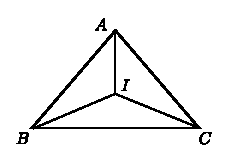
\includegraphics[scale=.85]{figures/1.eps}}}}
\newmng{ililx tirxBujada oLakeVMdarx $I$.}
\newmng{tirxBujada oLakeVMdarxvu A tirxBujada mUru bAhugaLiMda samadUra\-dalilxrutatxde.}
\end{entry}

\begin{entry}
\word{aMtaHkoVna divxBAjaka}
\gl{Internal Bisector of an Angle}
\mng{Akaqtiya oLakoVnavanunx adhiR\-suva reVKe.}
\newmng{\centerline{
\includegraphics[scale=.85]{figures/2.eps}}}
\smallskip
\newmng{udA~: $BI$ matutx $CI$ gaLu $\widehat{B}$ matutx $\widehat{C}$ gaLa divxBAjakagaLu.}
\end{entry}

\begin{entry}
\word{aMtaHkeSxVpa}
\gl{Interpolation}
\mng{oMdu sherxVDhiya athavA sherxVNiya naDuve biTiTxruva saMKeyx athavA pada\-gaLanunx niyamakekx anusAravAgi tuMbuva kirxye.}
\newmng{udA~: $+3$, $+5,\ldots,+9$ ililx $+7$ tuMbabeVku.}
\end{entry}

\begin{entry}
\word{aMtaHKaMDa}
\gl{Intercept}\newline
\mng{reVKAMtara.}
\newmng{eraDu athavA hecucx saraLareVKe\-gaLanunx beVroMdu saraLareVKe CeVdisi\-dAga eraDu reVKegaLa madheyx iruva BAga.}
\newmng{\centerline{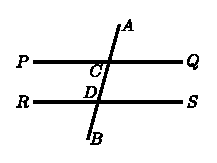
\includegraphics{figures/3.eps}}}
\newmng{citarxdalilx $AB$ CeVdakareVKe, $CD$ reVKAMtara athavA aMtaHKaMDa, $CD$ CeVdakareVKeya oMdu BAga.}
\end{entry}

\begin{entry}
\word{aMtaHtirxjayx}
\gl{Inradius}
\mng{oMdu Akaqtiya bAhugaLanunx sapxshiRsu\-vaMte aMtasathxvAgi racisida vaqtatxda tirxjayx.\break vaqtatxkeVMdarxdiMda bAhuvigiruva laMba\-dUra.}
\vskip .1cm
\newmng{\centerline{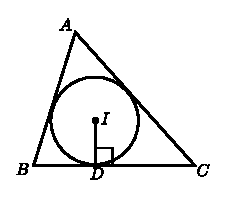
\includegraphics[scale=.9]{figures/4.eps}~~ \kern -1.4cm\raisebox{1.5cm}{$ID$ aMtaHtirxjayx}}}
\end{entry}

\begin{entry}
\word{aMtaHvaqtatx}
\gl{Incircle}
\mng{oLavaqtatx. Akaqtiya bAhugaLanunx sapxshiRsuvaMte eLediruva vaqtatx.}
\newmng{\centerline{\includegraphics[scale=.8]{figures/5.eps}}}
\newmng{$I$ keVMdarxvAgi $ID$ oLa tirxjayx iruvaMte eLeda vaqtatx.}
\end{entry}

\begin{entry}
\word{aMtaHsapxshaR}
\gl{Internal Contact}
\mng{oLasapxshaR.}
\newmng{sapxshiRsuva eraDu vaqtatxgaLa keVMdarxgaLu sapxshaRreVKeya oMdeV magugxlalilxdadxre A vaqtatxgaLu aMtaHsapxshiRsutatxve.}
\newmng{aMtasathxvAgi sapxshiRsuva vaqtatxgaLa keVMdarxgaLa naDuvina dUra $d$ Agidudx, A vaqtatxgaLa tirxjayxgaLu $R$ matutx $r$\break $(R>r)$ AgidAdxga}
\newmng{\centerline{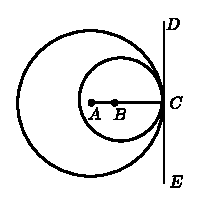
\includegraphics{figures/7.eps}}}

\medskip
\newmng{
\centering
\begin{tabular}{rl}
 & $AB=d$\\
  & $AC=R$\\
$d=R-r$ & $BC=r$
\end{tabular}}
\medskip

\newmng{citarxdalilx $AB=AC-BC$}
%\newmng{\centerline{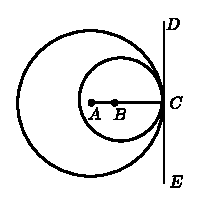
\includegraphics{figures/7.eps}}}
\end{entry}

\begin{entry}
\word{aMtara}
\gl{Distance}
\mng{eraDu biMdu\-gaLa ilalxve eraDu reVKegaLa naDuve iruva kaniSaTx dUra.}
\end{entry}

\begin{entry}
\word{aMtara}
\gl{Interval}
\mng{eraDu neYja saMKeyxgaLa naDuvina samasatx saMKeyxgaLa gaNa.}
\end{entry}

\begin{entry}
\word{aMtaragaNa}
\gl{Difference of Two Sets}
\mng{eraDu gaNagaLa vayxtAyxsa.}
\newmng{datatx $A$ matutx $B$ gaNagaLige saMbaMdhi\-sidaMte $B$ gaNadalilxruva gaNAMshagaLa horatAgi $A$ gaNadalilxruva gaNAMsha\-gaLa gaNa.}
\smallskip
\newmng{{\bf udA~:}}
\newmng{
\begin{center}
\begin{tabular}{r@{\,\,\,}c@{\,\,\,}l}
$A$ & = & $\{1,2,3,4,5,6\}$\\[3pt]
$B$ & = & $\{2,4,6,8\}$\\[3pt]
$A-B$ & = & $\{1,3,5\}$\\[3pt]
$A-B$ & = & $\{x/x\in A$ \ matutx \ $x\not\in B\}$
\end{tabular}
\end{center}}
\smallskip
\newmng{$A-B$ eraDu gaNagaLa vayxtAyxsa\-vanunx ililx sUcisidaMte venf citarxda\break mUlaka nirUpisabahudu.}
\newmng{\centerline{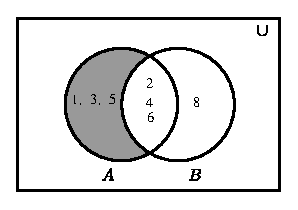
\includegraphics[scale=.9]{figures/8.eps}}}
\newmng{$A$ gaNadalilxruva gaNAMshagaLa hora\-tAgi $B$ gaNadalilxruva gaNAMshagaLa gaNaveV $B$ matutx $A$ gaNagaLa vayxtAyxsa, hiVge $B-A=\{8\}$, $B-A=\{x/x\in B$ matutx $x\not\in A\}$, $A-B\neq B-A$.}
\end{entry}

\begin{entry}
\word{aMtagaRta koVna}
\gl{Included Angle}
\mng{eraDu bAhugaLiMda EpaRTaTx koVna.}
\newmng{\centerline{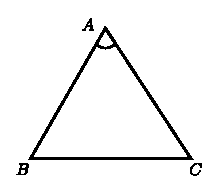
\includegraphics[scale=.9]{figures/9.eps}}}
\newmng{udA~: $AB$ matutx $AC$ bAhugaLiMda uMTAgiruva aMtagaRta koVna $B\widehat{A}C$.}
\end{entry}

\begin{entry}
\word{aMtagaRtagoLisu}
\gl{Include}
\mng{oLagoLuLxvaMte mADuvudu.}
\end{entry}

\begin{entry}
\word{aMtagaRta racane}
\gl{Inscribe}
\mng{aMtasathxvAgi racisuvike.}
\newmng{\centerline{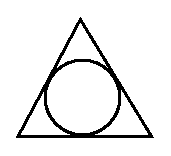
\includegraphics{figures/10.eps}}}
\newmng{oMdu AkaqtiyoLage matotxMdu Akaqtiyanunx racisuvudu.}
\newmng{udA~: citarxdalilx~ vaqtatxvu tirxBujadalilx aMtagaRtavAgide.}
\end{entry}

\begin{entry}
\word{aMtadaqRSiTx}
\gl{Intuition}
\mng{takaR, ciMtane\-gaLiMdalalxde keVvala aMtaH\-suPxraneyiMda hoLeva tiLivu.}
\end{entry}

\begin{entry}
\word{aMtadhARna biMdu}
\gl{Vanishing Point}
\mng{oMdeV samatala\-dalilxna elalx samAMtarareVKe\-gaLanUnx anaMta\-deDege vaqdidhxsidAga avu\-gaLelalx saMdhisuvaMte (saMgamisuvaMte) toVruva biMdu. I bagegx kepalxrf modalu tiLisida.}
\end{entry}

\begin{entry}
\word{aMtadhARna reVKe}
\gl{Vanishing Line}
\mng{oMdu samatalavu\break \hbox{tanage} samAnAMtaravAgiruva samatalagaLanunx anaMtadalilx saMdhisu\-vaMte toVruva reVKe.}
\end{entry}

\begin{entry}
\word{aMtalaRMba}
\gl{Off Set}

\smallskip
\mng{\centerline{\includegraphics[scale=.9]{figures/11.eps}}}
\newmng{catuBuRjada aBimuKa shaqMga\-gaLiMda kaNaRkekx eLeda laMbadUra. citarxdalilx $BE$ matutx $DF$ gaLu aMta\-laRMbagaLu.}
\end{entry}

\begin{entry}
\word{aMtavaRkarx catuBuRja}
\gl{Concave Quadrilateral}
\mng{nimanx catuBuRja. oMdu koVnavu saraLA\-dhikakoVnavAgiruva catuBuRja. oMdu kaNaR Akaqtiya horagaDe iruva catuBuRja.}
\newmng{\centerline{\includegraphics[scale=.9]{figures/12.eps}}}
\newmng{hiVge $ADBC$ nimanx catuBuRja. $DC$ kaNaR Akaqtiya horagide.}
\end{entry}

\begin{entry}
\word{aMtavaRkarx bahuBujAkaqti}
\gl{Concave Polygon}
\mng{oLabAgida bahuBujAkaqti oMdu athavA hecucx koVnagaLu saraLAdhikakoVnagaLAgi\-ruva bahuBujAkaqti. oMdu athavA hecucx kaNaRgaLu Akaqtiya hora\-gaDeyiruva bahuBujAkaqti.}
\vskip .1cm
\newmng{\centerline{\includegraphics[scale=.95]{figures/13.eps}}}
\vskip .1cm
\newmng{I citarxdalilx $AC$ kaNaR horagide.}
\end{entry}

\begin{entry}
\word{aMtavaqRtatx}
\gl{Incircle}
\mng{noVDi - aMtaHvaqtatx.}
\end{entry}

\begin{entry}
\word{aMtavaRhana utapxnanx}
\gl{Injective Function}
\mng{oMdu-oMdu citarxNa {\rm One One Mapping.}}
\newmng{$f:A\to B$ eMba saMbaMdha\-dalilx beVre beVre aMsha\-gaLa parxtibiMbagaLu beVre beVre Agiruva citarxNa.}
\newmng{\centerline{\includegraphics{figures/14.eps}}}
\newmng{$f:A\to B$ oMdu-oMdu utapxnanx.}
\newmng{$A$ yiMda $B$ ge iruva oMdu-\-oMdu citarxNa $A=\{a,b,c\}$, $B=\{1,2,3\}$ AgidAdxga $a\to 1$, $b\to 2$, $c\to 3$ idu $A$ yiMda $B$ ge nirUpisiruva oMdu-\-oMdu citarxNa.}
\end{entry}

\begin{entry}
\word{aMtasathx bahuBujAkaqti}\newline
\gl{Inscribed Polygon}

\smallskip
\mng{\centerline{\includegraphics{figures/15.eps}}}
\newmng{citarxdalilxruva $ABCDEF$ daMte oMdu bahuBujA\-kaqtiya elalx shaqMgagaLU oMdeV vaqtatx pari\-dhiya meVliruvaMte racisida bahuBujA\-kaqti aMtasathx bahuBujAkaqti.}
\end{entry}

\begin{entry}
\word{aMtasAthxBimuKakoVna}
\gl{Interior Opposite Angle}\newline
\mng{oLa eduru koVna.}
\newmng{oMdu Akaqtiya horakoVnada oLa eduru koVna.}
\vskip .1cm
\newmng{\centerline{\includegraphics{figures/16.eps}}}
\vskip .1cm
\newmng{citarxdalilx $x$, $y$\,gaLu $z$\,na aMta\-sAthxBi\-muKakoVna.}
\newmng{tirxBujada yAvudAdaroMdu bAhuvanunx vaqdidhx\-sidAga uMTAguva horakoVnavu aMtasAthxBimuKa koVnagaLa motatxkekx sama hiVge\break $\widehat{z}=\widehat{x}+\widehat{y}$, $A\widehat{C}D=A\widehat{B}C+B\widehat{A}C$.}
\vskip .1cm
\newmng{\centerline{\includegraphics{figures/17.eps}}}
\vskip .1cm
\newmng{vaqtitxVya catuBuRjadalilx yAvu\-dAdaroMdu bAhuvanunx vaqdidhxsi\-dAga uMTAguva horakoVna aMtasAthxBimuKa koVnakekx sama. $D\widehat{C}E=B\widehat{A}D$.}
\end{entry}

\begin{entry}
\word{aMtayx}
\gl{End}
\mng{kone, tudi.}
\end{entry}

\begin{entry}
\word{aMtayx padagaLu}
\gl{Extremes}
\mng{samAnupAta\-dalilxna modalina matutx kaDeya padagaLu.}
\newmng{udA~: $1:2=4:8$ eMba samAnapAtadalilx $1$ matutx $8$ aMtayx\-padagaLu.}
\end{entry}

\begin{entry}
\word{aMtayxbiMdu}
\gl{Terminal Point}
\mng{kaTaTxkaDeya biMdu.}
\end{entry}

\begin{entry}
\word{aMtArASiTxrXVya dinAMka reVKe}
\gl{International date line}
\mng{utatxra dakiSxNa dhurxvagaLanunx saMdhisu\-vaMte goVLada meVlemxY meVle eLeda kAlapxnika reVKe. $180^{\circ}$ reVKAMsha vaqtatx.}
\end{entry}

\begin{entry}
\word{aMdAju}
\gl{Estimate}
\mng{Uhisida parimANa, belekaTuTx. saMKeyx motatx modalAdavugaLa Uhe.}
\end{entry}

\begin{entry}
\word{aMdAju bele}
\gl{Estimated Value}
\mng{saninxhita bele. udA~: $36$ ra aMdAju bele $40$ ($10$ kekx samiVpa).}
\end{entry}

\begin{entry}
\word{aMsha}
\gl{Part}
\mng{BAga. beVre~beVre saMdaBaRgaLalilx idanunx upayoVgi\-sutAtxre. $33$ ra aMdAju bele $30$. BinanxrAshiyanunx bareyu\-vAga gereya meVlABx\-gada saMKeyx. $\frac{2}{3}$~ralilx $2$ aMsha. ($10$ kekx samiVpa CeVdadiMda sUcita\-vAda BAga\-gaLalilx eSuTx BAga\-gaLanunx tegedukoMDide eMbudanunx aMsha sUcisutatxde) mAtaqkeyalilxruva saMKeyxgaLu mAtaqkeya aMshagaLu.}
\newmng{$\left[\begin{array}{cc} 1 & 2\\ 4 & 8\end{array}\right]$ ralilx $1$, $2$, $4$, $8$ mAtaqkeya aMshagaLu. $1$ Digirx eMbudu laMbakoVnada $90$ neya oMdu aMsha. gaNa $A=\{a,b,c\}$ AdAga $a$, $b$, $c$ gaLu $A$ gaNadalilxruva aMshagaLu.}
\end{entry}

\begin{entry}
\word{aMshada parxtibiMba}
\gl{Image of the Element}
\mng{keSxVtarxdalilxna aMshadoMdige sahakeSxVtarxdalilxna aMsha\-vanunx jotegUDisuvudeV keSxVtarxdalilxna aMshada parxtibiMba. udA~: $A$ matutx $B$ eraDu gaNagaLu.}
\newmng{\centerline{\includegraphics{figures/18.eps}}}
\newmng{$f:A\to B$ oMdu utapxnanx\-vAgirali.}
\newmng{$f(a)=1$, $f(b)=2$, $f(c)=3$.}
\newmng{$B$ yalilxruva parxtiyoMdu aMshavU $A$ ya oMdu aMshada parxtibiMba\-vAgirutatxde. $a$ ya parxtibiMba $1$.}
\end{entry}

\begin{entry}
\word{akaraNiVkaraNa}
\gl{Rationalisation}
\mng{pari\-meV\-yiV\-karaNa.
oMdu karaNiyanunx matotxMdu karaNi\-yiMda guNisi, BAgalabadhx saMKeyxyanunx paDeyuva karxma. udA~: $\sqrt{5}\times \sqrt{5}=5$.~~ {\bf noVDi - karaNa}.}
\end{entry}

\begin{entry}
\word{akaraNiVkAraka}
\gl{Rationalising}
\mng{parimeVya\-kAraka.}
\newmng{akaraNiVkaraNa naDedAga oMdu karaNiyanunx inonxM\-dara akaraNiV\-kAraka enunxtetxVve.}
\vskip .15cm
\newmng{
\begin{tabular}{@{}r@{\;\,}l@{}}
udA~: & $\sqrt{x}\times \sqrt{x}=x$\\[2pt]
      & $x$ oMdu BAgalabadhx saMKeyx\\[2pt]
      & $\sqrt{x}$ na akaraNiVkAraka $\sqrt{x}$
\end{tabular}}

\smallskip
\newmng{
\begin{center}
\tabcolsep=8pt
\renewcommand{\arraystretch}{1.55}
\begin{tabular}{|c|c|}
\hline
{\bf karaNi} & {\bf akaraNiVkAraka}\\
\hline
$a\sqrt{x}$ & $\sqrt{x}$\\
$x+\sqrt{y}$ & $x-\sqrt{y}$\\
$x-\sqrt{y}$ & $x+\sqrt{y}$\\
$\sqrt{x}+\sqrt{y}$ & $\sqrt{x}-\sqrt{y}$\\
$\sqrt{x}-\sqrt{y}$ & $\sqrt{x}+\sqrt{y}$\\
$a\sqrt{x}+b\sqrt{y}$ & $a\sqrt{x}-b\sqrt{y}$\\
$a\sqrt{x}-b\sqrt{y}$ & $a\sqrt{x}+b\sqrt{y}$\\
$\sqrt{x+y}$ & $\sqrt{x+y}$\\
$\sqrt{x-y}$ & $\sqrt{x-y}$\\
\hline
\end{tabular}
\end{center}}
\end{entry}

\begin{entry}
\word{akeVMdarx}
\gl{Non-Centre}
\mng{keVMdarx\-valalxda.}
\end{entry}

\begin{entry}
\word{akarxma}
\gl{Irregular}
\mng{karxmavalalxda.}
\end{entry}

\begin{entry}
\word{akaSx}
\gl{Axis}
\mng{akaSxreVKe.}
\smallskip
\newmng{\centerline{\includegraphics{figures/19.eps}}}
\smallskip
\newmng{oMdu vasutxvina madhayxdiMda hAdu hoVguva reVKe. oMdu \hbox{vasutxvu} oMdu biMdu (keVMdarx)vina \hbox{sutatx} sututx\-titxruvAga, A biMduvina \hbox{mUlaka} hAduhoVguva reVKe.}
\end{entry}

\begin{entry}
\word{akaSxra sahaguNaka}
\gl{Literal Coefficient}
\mng{oMdu biVjapadadalilx saMKeyxya muMde baruva avayxkAtxkaSxra. udA~: $4a$ eMbudaralilx $a$ eMbudu $4$\,ra akaSxra sahaguNaka.}
\end{entry}

\begin{entry}
\word{akASxMsha}
\gl{Latitude}
\mng{BU sama\-BAjaka \hbox{vaqtatxkekx} samAMtara\-vAgi eLedaMtiruva kAlapxnika vaqtatxda meVlina koVniVya aMtara. I aMtaravanunx sama\-BAjakada utatxrakekx ilalxve dakiSxNakekx iMtiSuTx Digirx eMdu sUcisalAguvudu.}
\vskip .1cm
\newmng{\centerline{\includegraphics{figures/20.eps}}}
\vskip .1cm
\newmng{akASxMsha matutx reVKAMshagaLu \hbox{BUmiya} meVlina sathxLagaLanunx sUci\-suva koVna nideVRshakagaLu.}
\end{entry}

\begin{entry}
\word{agala}
\gl{Breadth}
\mng{aDaDxgala; vasutx\-vina aDaDxLate. oMdu AyatAkArada samatalada udadxgaLa naDuvina laMba\-dUra.}
\end{entry}

\begin{entry}
\word{acaraguNa}
\gl{Invariant Pro-\-perty}
\mng{badalA\-gada gaNa. sithxtisAthxpaka calaneyiMda mApaRDada gaNa.}
\end{entry}

\begin{entry}
\word{acucxvidhAna}
\gl{Wedge Method}
\mng{saMKeyxgaLanunx sUcisalu kirx.pU. $5000$ diMda kirx.pU. $3000$ da tanaka rUDhiyalilxdadx oMdu karxma.}
\end{entry}

\begin{entry}
\word{ajAcnxtasaMKeyx}
\gl{Unknown Number}
\mng{avayxkatxsaMKeyx. niKaravAda bele\-yilalxda saMKeyx. udA~: $x+y=8$ ralilx $x$ matutx $y$ gaLu ajAcnxta saMKeyx\-gaLu.}
\end{entry}

\begin{entry}
\word{aDi}
\gl{Foot}
\mng{birxTiSf padadhxtiyalilx udadxLateya mUlamAna, gajada $\frac{1}{3}$ BAga. $1$ aDi $=12$ aMgula. modalalilx manuSayx pAdada aLate\-yanunx AdhAravAgiTuTxkoMDidudxda\-riMda I hesaru baMdirabahudu.}
\end{entry}

\begin{entry}
\word{aDaDxkoyatx}
\gl{Cross Section}
\mng{oMdu Gana\-vasutxvanunx samatala\-voMdariMda aDaDxvAgi katatxrisidAga kANuva A Ganada muKa athavA meVlemxY.}
\end{entry}

\begin{entry}
\word{aDaDxgala}
\gl{Span}
\mng{oMdu tudi\-yiMda matotxMdu tudiyavaregina vAyxpitx.}
\end{entry}

\begin{entry}
\word{aDaDxgere cekf}
\gl{Crossed Cheque}
\mng{reVKi\-siruva dhanA\-deVsha patarx, kArxsfcekf haNavanunx naga\-dAgi pAvati mADade AdeVsha\-vititxruvavara lekakxkekx jamA mADu\-vaMte \hbox{sUcane} niVDi, eDaBAgada meVlutxdi\-yalilx eraDu samAMtara aDaDxgere eLediruva cekf.}
\end{entry}

\vskip .1cm

\begin{entry}
\word{aDaDxreVKe}
\gl{Horizontal Line}
\mng{kiSxtijareVKe, hArijareVKe, talareVKe, laMbareVKege laMbavAgiruva reVKe.}
\end{entry}

\vskip .1cm

\begin{entry}
\word{aDaDxsAlina mAtaqke}
\gl{Row Vector, Row Matrix}
\mng{talasAlina athavA aDaDxsAlina dishAyukatx pari\-mANa. tala sAlina dikf parimANa.}
\newmng{oMdu aDaDxsAlu iruva mAtaqke. udA~: $P=\left[2 \ \ 3 \ \ 4\right]$.}
\end{entry}

\vskip .1cm

\begin{entry}
\word{aDaDxsAlu}
\gl{Row}
\mng{talasAlu.}
\newmng{$A=\left[\begin{matrix} 1 & 2 & 3\\[2pt] 4 & 5 & 6\end{matrix}\right]$ I mAtaqkeyalilx aDaDxsAlina aMshagaLu $1$, $2$, $3$ matutx $4$, $5$, $6$.}
\end{entry}

\vskip .1cm

\begin{entry}
\word{aDaDxsatxMBAleVKa}
\gl{Horizontal Bar Graph}
\mng{satxMBAleVKa\-vanunx keLage toVrisiruvaMte aDaDxvAgi racisidAga doreyuva satxMBanakeSx.}

\smallskip
\newmng{\raisebox{1cm}{taragati}~ {\includegraphics[scale=.92]{figures/21.eps}}}
\newmng{\centerline{~~~~vidAyxthiRgaLu}}
\end{entry}

\vskip .1cm

\begin{entry}
\word{aDaDxhAyuva nakeSx}
\gl{Traversable Figure}
\mng{pAravAhaka jAlAkaqti.}
\newmng{oMdu siVsada kaDiDxya tudiyanunx kAgadadiMda meVlakekx etatxde matutx omemx eLeda kaMsada meVle matetx eLeyade racisabahudAda citarx.}
\vskip .15cm
\newmng{\centerline{\includegraphics{figures/67.eps}}}
\vskip .1cm
\newmng{ililx sUcisidaMte anukarxma\-vAgi\break \eng{1, 2, 3, 4, 5, 6, 7, 8} matutx $9$ eMba mAgaRgaLa mUlaka hAdu I Akaqtiyanunx racisabahudu. AdadxriMda idoMdu pAravAhaka jAlAkaqti.}
\newmng{yAvAgalU~ {\rm(1)}~ datatx jAlAkaqti pAravAhaka jAlAkaqtiyAgabeVkA\-dare adaralilx eraDu athavA eraDa\-kikxMta kaDime besa saMpAta biMdugaLu irabeVku.}
\vskip .1cm
\newmng{{\rm(2)}~ datatx jAlAkaqti pAravAhaka jAlAkaqtiyeMdu pariVkiSxsalu besa saMpAta biMduviniMda pArxraMBisa\-beVku.}
\vskip .1cm
\newmng{{\rm(3)}~ sama saMpAta biMdugaLiruva pAravAhaka jAlAkaqtiyalilx pArxraMBa matutx aMtayx oMdeV biMdu\-vinalilx EpaRDutatxde.}
\vskip .1cm
\newmng{{\rm(4)}~ eraDu besa \hbox{saMpAta} biMdu\-gaLiruva pAravAhaka jAlAkaqtiyalilx pArxraMBa oMdu besa saMpAta biMdu\-vi\-nalUlx, konegoLuLxvudu \hbox{inonxMdu} besa saMpAta biMdu\-vinalUlx Agirutatxde.}
\end{entry}

\begin{entry}
\word{aNitayugamx}
\gl{Ordered Pair}
\mng{sakarxmayugamx, karxmayugamx.}
\newmng{reVKAtamxka samiVkaraNada nideVRshAMka\-gaLanunx sUci\-suva karxma.}
\newmng{$(x,y)$ rUpadalilx bareda samiV\-karaNada $X$ matutx $Y$ nideVR\-shAMkagaLa joVDigaLu. hiVge $Y=2x+1$ na samiVkaraNada sakarxma\-yugamxgaLu $(0,1)$, $(1,3)$, $(2,5)$ itAyxdi.}
\end{entry}

\begin{entry}
\word{ataLareVKegaLu}
\gl{\hbox{Skew Lines}}
\mng{BinanxtaLiVya reVKegaLu. sUkxyXreVKe\-gaLu, ataLa reVKegaLu, oMdeV samataladalilxlalxda eraDu reVKegaLu. ivu elilxyU saMdhisuvudilalx.}
\vskip .1cm
\newmng{\centerline{\includegraphics[scale=.9]{figures/69.eps}}}
\vskip .1cm
\newmng{tirxkoVna paTaTxkadalilx $(OA,BC)$, $(OB,AC)$, $(OC,AB)$ gaLu Binanx\-taliVya reVKegaLu.}
\end{entry}

\begin{entry}
\word{atiparavalaya}
\gl{Hyperbola}
\mng{laMbavaqtitxVya yugamxshaMku\-vanunx {\eng{(double cone)}} adara keVMdarx\-diMda eraDU kaDeyU samatala CeVdhisi\-dAga talada CeVdaveV atipara\-valaya. hiVge CeVdisidAga mUru bageya vakarxreVKegaLa peYki atipara\-valaya oMdu. uLideraDu oMdu diVGaR\-vaqtatx (elilxpfsx); matotxMdu para\-valaya {\eng{(parabola)}}. atipara\-valaya eraDu hAlegaLiruva \hbox{vivaqta} vakarxreVKe {\eng{(open curve)}}. ati\-paravalayada utekxVMdarxte {\eng{(eccentricity)}} $1$ kikxMta adhika.}
\newmng{\centerline{\includegraphics[scale=.9]{figures/70.eps}}}
\newmng{
\begin{center}
\begin{tabular}{r}
citarxdalilx $H$-$H$ atiparavalaya\\
$A$-anaMta sapxshaRkagaLu.
\end{tabular}
\end{center}}
\end{entry}

\begin{entry}
\word{adisha parimANa}
\gl{Scalar Quantity}
\mng{avAhaka\-rAshi.}
\newmng{dishArahitavAgidudx keVvala pari\-mANa mAtarx iruva BwtaparimANa. udA~: java.}
\end{entry}

\begin{entry}
\word{adisha mAtaqke}
\gl{Scalar Matrix}
\mng{parimANa saMKAyxyata.}
\newmng{vagaR mAtaqkeya parxdhAna kaNaRda aMshagaLelalxvU samavAgiruva matutx uLidelalx aMshagaLu sonenxyAgi\-ruva mAtaqke.}
\newmng{udA~: $P=\begin{bmatrix} 2 & 0 & 0\\ 0 & 2 & 0\\ 0 & 0 & 2\end{bmatrix}$}
\end{entry}

\begin{entry}
\word{adhika}
\gl{Excess}
\mng{parimANadalilx Agali, saMKeyx\-yalAlxgali hecAcxda.}
\end{entry}

\begin{entry}
\word{adhikakoVna}
\gl{Obtuse Angle}
\mng{vishAlakoVna.}
\newmng{$90^{\circ}$giMta hecucx $180^{\circ}$giMta kaDime parimANa iruva koVna.}
\vskip .1cm
\newmng{\centerline{\includegraphics[scale=.9]{figures/74.eps}}}
\vskip .1cm
\newmng{\centerline{citarxdalilx $ABC$ adhikakoVna.}}
\end{entry}

\begin{entry}
\word{adhikakoVna tirxBuja}
\gl{Obtuse Angled Triangle}
\mng{vishAlakoVna tirxBuja.}
\newmng{tirxBujada oMdu koVna. vishAla\-koVnavAgiruva tirxBuja.}
\vskip .1cm
\newmng{\centerline{\includegraphics[scale=.9]{figures/75.eps}}}
\vskip .1cm
\newmng{citarxdalilxruva $\triangle ABC$ vishAla\-koVna tirxBuja vishAla\-koVnakekx edurAgiruva bAhu uLideraDu bAhugaLigiMta doDaDxdAgirutatxde. oMdu vishAla\-koVna tirxBujadalilx yAvAgalU oMdeV oMdu vishAlakoVnaviru\-tatxde.}
\end{entry}

\begin{entry}
\word{adhikatama}
\gl{Maximum}
\mng{gariSaThx, atayxdhika. atayxMta hecucx paramA\-vadhiya, atayxMta hecicxna pari\-mANa.}
\end{entry}

\begin{entry}
\word{adhikabele}
\gl{Premium; Above Par}
\mng{pirxVmiyaM bele, hecicxna bele.}
\newmng{udA~: $100$ rU. \hbox{muKabeleya} oMdu SeVru $120$ rU. ge mArATa\-vAgutitxdadxre adu adhika bele SeVru.}
\end{entry}

\begin{entry}
\word{adhikavaSaR}
\gl{Leap Year}
\mng{parxti nAlukx vaSaRkokxMdAvatiR baruva $366$ divasagaLa vaSaR. A vaSaRda Pebarxvari tiMgaLalilx $29$ divasagaLiru\-tatxve. datatx isaviyu $4$ riMda matutx $400$ riMda nisheshxVSavAgi BAgavAdare A vaSaR adhikavaSaR.}
\end{entry}

\begin{entry}
\word{adhicakarx}
\gl{Epicycle}
\mng{kirx.sha. sumAru $7$neya shata\-mAnadalilx jiVvisida IjipiTxna TAlemi eMba KagoVLavijAcnxni parxtipAdisida sidAdhxMtada parxkAra doDaDx \hbox{vaqtatxda} paridhiya meVle calisuva keVMdarx\-vuLaLx saNaNxvaqtatx doDaDx\-vaqtatxda hesaru. DePareMTf. AkAshagoVLada \hbox{keVMdarx} BUmi. adara sutatxlU caMdarx, budha, shukarx, sUyaR muMtAdavu adeV karxmadalilx pariBarxmisutitxve eMda\break TAlemiya sidAdhxMtavanunx gaNita\-riVtayx samathiR\-salu adhicakarxda Avashayxkate uMTAyitu. parxkaqtadalilx adhicakarxkekx keVvala aitihAsika mahatatxvX mAtarx ide.}
\smallskip
\newmng{\centerline{\includegraphics{figures/79.eps}}}
\smallskip
\newmng{doDaDx vaqtatxda paridhiya meVle calisuva keVMdarxvuLaLx saNaNx vaqtatx. (TAlemiya sidAdhxMtada parxkAra)}
\end{entry}

\begin{entry}
\word{adhivAyxpita}
\gl{Over Lapping}
\mng{oMdanonxMdu AvarisikoMDiruva vagARMtara. oMdeV mwlayx eraDu vagARMtaradalUlx baMdiruvudu.}
\newmng{
\begin{center}
\begin{tabular}{r@{\qquad}|c|}
\cline{2-2}
udA~: & vagARMtara\\
\cline{2-2}
      & {\rm 1 - 10}\\
      & {\rm 10 - 20}\\
      & {\rm 20 - 30}\\
\cline{2-2}
\end{tabular}
\end{center}}
\newmng{ililx $10$ eMba mwlayxvu {\rm 1 - 10} matutx {\rm 10 - 20} I eraDu vagARM\-taragaLalilx ide.}
\end{entry}

\begin{entry}
\word{adhAyxroVpaNa vidhAna}
\gl{Method of Super-Position}
\mng{samAroVpa karxma.}
\newmng{hoVlisuva saluvAgi oMdu citarx\-vanunx matotxM\-dara meVle iDuvudu samAroVpa. I riVtiyAgi sAmayx\-vanunx pariVkiSxsuva vidhAnaveV adhAyx\-roVpaNa vidhAna.}
\end{entry}

\begin{entry}
\word{adhoVparibaMdha}
\gl{\hbox{Lower Bound}}
\mng{keLagina miti.}
\end{entry}

\begin{entry}
\word{adhaR}
\gl{Half}
\mng{are.}
\newmng{oMdu vasutxvina athavA rAshiya eraDu samaBAga\-gaLalilx oMdu BAga. $\frac{1}{2}$ (eraDaneV oMdu BAga).}
\end{entry}

\begin{entry}
\word{adhaRgoVLa}
\gl{Semisphere}
\mng{goVLada adhaR\-BAga.}
\newmng{\centerline{\includegraphics{figures/84.eps}}}
\newmng{$ABC$ adhaRgoVLa.}
\newmng{ToLuLx adhaRgoVLada horameY visitxVNaR = $2\pi r^{2}$}
\newmng{Gana (gaTiTx) adhaRgoVLada oTuTx horameY visitxVNaR = $3\pi r^{2}$}
\newmng{adhaRgoVLada GanaPala = $\frac{2}{3}\pi r^{3}$.}
\end{entry}

\begin{entry}
\word{adhaRparidhi}
\gl{Semi Circumference}
\mng{vaqtatx paridhiya adhaRBAga.}
\end{entry}

\begin{entry}
\word{adhaRvASiRka pirxVmiyamf}
\gl{Half Yearly Premium}
\mng{Aru tiMgaLigomemx kaTuTxva vimekaMtu.}
\end{entry}

\begin{entry}
\word{adhaRvaqtatx}
\gl{Semi Circle}\newline
\mng{\hbox{vaqtAtxdhaR.}}
\newmng{vAyxsavu vaqtatxvanunx samadivxBAgisu\-tatxde. I samaBAga\-gaLeV adhaRvaqtatx\-gaLu. adhaRvaqtatxdalilxna paridhikoVna oMdu laMbakoVna.}
\newmng{\centerline{\includegraphics{figures/87.eps}}}
\vskip .2cm
\newmng{$O$ keVMdarxvuLaLx vaqtatxdalilx $B\widehat{A}C$ adhaR\-vaqtatxdalilxna koVna $B\widehat{A}C=90^{\circ}$.}
\end{entry}

\vskip .15cm

\begin{entry}
\word{adhiRsu}
\gl{Bisect}
\mng{samadivxBAgisu.}
\newmng{koVna athavA bAhuvanunx eraDu samaBAgagaLanAnxgi mADuvudu.}
\end{entry}

\vskip .2cm

\begin{entry}
\word{adhiRsuva reVKe}
\gl{Bisector}\newline
\mng{divxBAjaka, sama\-BAjaka.}
\newmng{saraLareVKe athavA koVnavanunx athavA Akaqtiyanunx samavAgi eraDu BAga mADuva reVKe.}
\vskip .25cm
\newmng{\centerline{\kern -.75cm\includegraphics[scale=.87]{figures/89.eps}}}
\end{entry}

\vskip .2cm

\begin{entry}
\word{anaMta}
\gl{Infinity}
\mng{koneyilalxda; aMtayx \hbox{ilalxdudx,} asaMKeyx; aparimita; anaMtavAda motatx. idara cihenx $\infty$.}
\end{entry}

\vskip .2cm

\begin{entry}
\word{anaMtagaNa}
\gl{Infinite Set}
\mng{aparimitagaNa; siVmitagaNa, gaNAMsha\-vanunx eNisalu asAdhayxvAda gaNa.}
\smallskip
\newmng{udA~: sAvxBAvika saMKAyxgaNa. $N=\{1,2,3,\-4,\ldots\}$.}
\end{entry}

\vskip .2cm

\begin{entry}
\word{anaMtasherxVNi}
\gl{Infinite Series}
\mng{anaMta aMsha\-gaLanunx hoMdiruva sherxVNi.}
\newmng{udA~: $1+2+3+\ldots$}
\end{entry}

\begin{entry}
\word{anaMtasapxshaRka}
\gl{Asymptote}
\mng{sAMta dUra\-dalelxlUlx sapxshiRsada Adare anaMtadalilx sapxshiRsuva reVKe.}
\end{entry}

\begin{entry}
\word{ananayxtA utapxnanx}
\gl{Identity Function}
\mng{$A$ yu oMdu gaNa\-vAgi\-rali, $f:A\to A$ \hbox{eMbudu} oMdu utapxnanxvAgidudx adaralilx parxti\-yoMdu aMshavU adeV aMshakekx parxti\-biMbavAgiruva \hbox{utapxnanx.} I \hbox{utapxnanx} yAvAgalU oMdu-\-meVlaNa utapxnanxvAgirutatxde.}
\vskip .1cm
\newmng{$f(x)=x \ \forall x\in A$}
\vskip .1cm
\newmng{udA~: gaNa $A=\{1,2,3\}$ Adare ananayxtA utapxnanx $f=\{(1,1),(2,2),(3,3)\}$}
\end{entry}

\begin{entry}
\word{ananayxtA saMbaMdha}
\gl{Identity Relation}
\mng{sArUpayx saMbaMdha.}
\newmng{idu savxyaMgaNa saMbaMdhada oMdu bage. $A$ gaNadalilx $R=\{(x,y)/x-y,\break x\in A, y\in A\}$ Agiruva \hbox{saMbaMdha}. udA~: $A=\{1,2,3\}$ Adare $R=\{(1,1),(2,2),(3,3)\}$.}
\end{entry}

\begin{entry}
\word{ananayxteya saMkeVta}
\gl{Identity Element}
\mng{savaRsamAnAMsha, ananAyxMsha.}
\end{entry}

\begin{entry}
\word{ananayx mAtaqke}
\gl{Identity Matrix; Unit Matrix}
\mng{ananayxsaMKAyxyata; EkakamAtaqke; GaTaka saMKAyxyata.}
\newmng{kaNaRmAtaqkeya parxdhAnakaNaRda aMshagaLu $1$ (oMdu) Agiruva mAtaqke.}
\newmng{idanunx $I$ eMba akaSxradiMda sUcisa\-lAgutatxde.}
\vskip .1cm
\newmng{$I=\begin{bmatrix} 1 & 0 & 0\\ 0 & 1 & 0\\ 0 & 0 & 1\end{bmatrix}$~ $I$ ananayx mAtaqke}
\end{entry}

\begin{entry}
\word{anApavataRyx rAshigaLu}
\gl{In Commensurable Quantities}
\mng{oMdanunx biTuTx beVre sAmAnayx apavataRnavilalxda saMKAyxrAshigaLu. udA~: $5,14,29$}
\end{entry}

\begin{entry}
\word{anAgata dinAMkada cekukx}
\gl{Post-Dated Cheque}
\mng{\hbox{pAva\-tige} hAjaru\-paDisida dinAMkakikxMta \hbox{muMdina} dinAMkada namUdane iruva cekf.}
\end{entry}

\begin{entry}
\word{anAvataR dashamAMsha}
\gl{Non-Terminating; Non Recurring Decimal}
\mng{koneyeMbu\-dilalxda matutx AvataRvalalxda dashamAMsha.}
\newmng{udAharaNe~:}
\vskip .1cm
\newmng{\kern -.1cm$\sqrt{2}=1\cdot 4~1~4~2~1~3~5~6~2\ldots$}
\end{entry}

\begin{entry}
\word{anidiRSaTx}
\gl{Indefinite}
\mng{anishicxta.}
\end{entry}

\begin{entry}
\word{anidhARraNiVya}
\gl{Indeterminate}
\mng{anidhAR\-rita.}
\newmng{beleyanunx sariyAgi nidhaRrisalu sAdhayxvAgade iruvaMtha niSapxtitxgaLu.}
\vskip .1cm
\newmng{udA~: $\frac{0}{0}$, $\frac{\infty}{\infty}$, $0^{
0}$, $\infty-\infty$, $1^{\infty}$. ivelalx anidhaRra\-NiVyagaLu.}
\end{entry}

\begin{entry}
\word{anishicxta}
\gl{Undetermined}\newline
\mng{tiVmARnavAgilalxda; aniNiVRta.}
\end{entry}

\begin{entry}
\word{anishicxtAthaRka heVLike}
\gl{Ambiguous Statement}
\mng{saMdigadhx nirU\-paNe.}
\newmng{datAtxMshagaLiMda eraDu beVre beVre tiVmARnagaLanunx paDeyalu sAdhayxte\-yiruva heVLike.}
\newmng{udA~: oMdu tirxBujada eraDu bAhugaLu matutx A bAhugaLiMda EpaRTaTx koVnavanunx koTATxga vishAla\-koVna athavA laGukoVna tirxBuja\-vanunx racisa\-bahudu.}
\end{entry}

\begin{entry}
\word{anukarxma}
\gl{Consecutive}\newline
\mng{karxmAgata.}
\end{entry}

\begin{entry}
\word{anukarxmakoVnagaLu}
\gl{Consecutive Angles}
\mng{anukarxma shaqMga\-gaLalilx uMTAguva koVna\-gaLu.}
\vskip .1cm
\newmng{\centerline{\includegraphics[scale=.9]{figures/106a.eps}}}
\vskip .1cm
\newmng{udA~: $ABCD$ catuBuRjadalilx $\widehat{A}$ matutx $\widehat{B}$, $\widehat{B}$ matutx $\widehat{C}\ldots$ itAyxdi anukarxmakoVnagaLu.}
\newmng{samAnAMtara catuBuRjada anukarxma\-koVnagaLu paripUraka.}
\vskip .1cm
\newmng{\centerline{\includegraphics[scale=.9]{figures/106b.eps}}}
\vskip .1cm
\newmng{$ABCD$ samAMtara catuBuRjadalilx $\widehat{A}+\widehat{B}=180^{\circ}$ itAyxdi.}
\end{entry}

\begin{entry}
\word{anukarxmavAgi}
\gl{Respectively}
\mng{adaradara saMbaMdha\-kakxnusAravAgi.}
\end{entry}

\begin{entry}
\word{anukarxma shaqMga}
\gl{Consecutive Vertex}
\mng{karxmA\-gata athavA karxmAnu\-gata shaqMgagaLu.}
\newmng{parxdakiSxNa athavA aparxdakiSxNa karxmadalilx ulelxVKisuva shaqMgagaLu.}
\vskip .1cm
\newmng{\centerline{\includegraphics[scale=.95]{figures/108.eps}}}
\vskip .1cm
\newmng{udA~: $PQRS$ catuBuRjadalilx $P$ matutx $Q$ oMdu jote anukarxma shaqMgagaLu.}
\end{entry}

\begin{entry}
\word{anukUla vitaraNe}
\gl{Fair Distribution}
\mng{niSapxkaSxpAtavAda vitaraNe; takakxmaTiTxna parxmANadalilx haMcuvudu.}
\end{entry}

\begin{entry}
\word{anukarxma saMKeyxgaLu}
\gl{Consecutive Numbers}
\mng{karxmAgata saMKeyxgaLu.}
\newmng{datatxsaMKeyxge oMdanunx kUDidare baruva muMdina saMKeyx.}
\newmng{udA~:~$10,11,12,13,\ldots$~itAyxdi.}
\newmng{BAratada gaNitajacnx AyaRBaTa karxmA\-gata saMKeyxgaLa vagaRgaLa motatx matutx GanagaLa motatxvanunx kaMDu\-hiDiyuva sUtarxvanunx nirUpisida.
\begin{align*}
&1^{2}+2^{2}+3^{2}+\cdots+n^{2}\\ 
&\qquad\quad = \frac{1}{6}n(n+1)(2n+1)\\
&1^{3}+2^{3}+3^{3}+\cdots+n^{3}\\
&\qquad\quad = \left[\frac{1}{2}n(n+1)\right]^{2}
\end{align*}}
\end{entry}

\begin{entry}
\word{anugata}
\gl{Continued}\newline
\mng{muMduvareda.}
\end{entry}

\begin{entry}
\word{anugamana}
\gl{Induction}
\mng{nidiRSaTx\-vAda udA\-haraNegaLiMda oMdu sUtarx athavA niyamagaLanunx nirUpisuva karxma.}
\newmng{udAharaNe~:
\begin{center}
\tabcolsep=1.5pt
\renewcommand{\arraystretch}{1.3}
\begin{tabular}{|c|c|c|c|c|}
\hline
vaqtatx & paridhi & vAyxsa & $\dfrac{\text {paridhi}}{\text {vAyxsa}}$ & niyatAMka\\
\hline
1 & $c_{1}$ & $d_{1}$ & $\frac{c_{1}}{d_{1}}$ & $K_{1}$\\
2 & $c_{2}$ & $d_{2}$ & $\frac{c_{2}}{d_{2}}$ & $K_{2}$\\
- & - & - & - & -\\
\hline
\end{tabular}
\end{center}}
\newmng{$K_{1}$, $K_{2}\ldots$ itAyxdigaLu niya\-tAMshagaLu. I udA\-haraNeyalilx A niyatAMka $\pi$ ge sama.}
\end{entry}

\begin{entry}
\word{anuparxtijecnx}
\gl{Rider}
\mng{oMdu parxti\-jecnxge parxtayxkaSxvAgi athavA paroVkaSxvAgi saMbaMdhapaTaTx adara tatatxvXgaLa meVle AdhAravAda parxshenx. upaparxtijecnx.}
\end{entry}

\begin{entry}
\word{anupAta}
\gl{Ratio}
\mng{parxmANa. sonenx\-yalalxda eraDu sajAtiVya pari\-mANagaLalilx oMdu parimANa \hbox{matotxMdu} parxmANada eSuTx paTuTx ide eMbudanunx sUcisuva shudadhx saMKeyx.}
\newmng{udA~: $3:6$}
\end{entry}

\begin{entry}
\word{anupAtiVya haMcike}
\gl{Proportional Division}
\mng{oMdu datatx parxmA\-Nakekx anusAravAgi, oMdu motatxvanunx eraDu athavA adakikxMta hecucx BAgagaLAgi viBAgisuva karxma.}
\newmng{udA~: $250$ nunx $2:3$ anu\-pAtadalilx haMcidAga baruva BAga\-gaLu $100$ matutx $150$.}
\end{entry}

\begin{entry}
\word{anubaMdha}
\gl{Appendix}
\mng{garxMthada koneyalilx oLagina vividha viSaya\break\-gaLige saMbaMdhapaTaTxMte koDuva\break visheVSa viSayagaLa paTiTx athavA nirUpaNe.}
\newmng{udA~: niGaMTina koneyalilx \hbox{koDuva} nuDigaTuTxgaLu, sUtarxgaLu itAyxdigaLa paTiTx.}
\end{entry}

\begin{entry}
\word{anubadadhx saMkiVNaR saMKeyx}
\gl{Conjugate of a Complex Number}
\mng{$z=a+ib$ Adare $\overline{z}=a-ib$ eMba saMKeyxyu $z$ na anubadadhx\break saMkiVNaR saMKeyx.}
\end{entry}

\begin{entry}
\word{anumAna}
\gl{Infer}
\mng{anu\-gamana athavA niga\-mana vidhAnadiMda mADuva Uhe athavA maMDi\-suva aBipArxya.}
\end{entry}

\begin{entry}
\word{anumita}
\gl{Corollary}
\mng{upa\-parxmeVya, upa\-sidAdhxMta.}
\newmng{parxmeVyagaLanunx nirUpisuvAga kaMDubaruva athavA nirUpisida baLika avugaLa sahAyadiMda takaR\-mADabahudAda \hbox{sidAdhxMta}. parxmeVyadiMda sulaBa\-vAgi UhisabahudAda nijAMshada nirU\-paNe.}
\newmng{udA~: EkapAdada meVle oMdeV jote samAM\-tara saraLa\-reVKegaLa naDuve iruva samAM\-tara catuBuRjagaLu visitxVNaRdalilx samavAgiruvudu eMba parxmeVyada upaparxmeVya samapAdagaLa meVle oMdeV jote samAMtara saraLa\-reVKegaLa naDuve iruva samAM\-tara catuBuRjagaLu visitxVNaRdalilx samavAgiruvuvu.}
\end{entry}

\begin{entry}
\word{anurUpakoVna}
\gl{Corresponding Angle}
\mng{saMvAdikoVna, sadaqshakoVna.}
\newmng{eraDu saraLareVKegaLanunx CeVdaka katatxrisidAga CeVdaka\-reVKeya oMdeV magugxlalilxruva hora matutx oLa eduru koVnagaLu.}
\vskip .1cm
\newmng{\centerline{\kern -.4cm\includegraphics{figures/119.eps}}}
\vskip .1cm
\newmng{saraLareVKegaLu samAMtaravAgidAdxga anurUpa\-koVnagaLu parasapxra sama.}
\newmng{citarxdalilx nAlukx jote anurUpa koVnagaLive. $a$ matutx $b$ oMdu jote anurUpakoVnagaLu. $l_{1} \|\, l_{2}$ Agi\-dAdxga $\widehat{a}=\widehat{b}$.}
\end{entry}

\vskip .1cm

\begin{entry}
\word{anurUpate}
\gl{Analogy}
\mng{sAdaqshayx.}
\end{entry}

\vskip .1cm

\begin{entry}
\word{anurUpavAgiru}
\gl{To Correspond}
\mng{hoMdikeyAgu, hoVlu, saMvAdiyAgu.}
\end{entry}

\vskip .1cm

\begin{entry}
\word{anuloVma mApuR}
\gl{Direct Variation}
\mng{neVra mApuR.}
\newmng{mApiRnalilx savxtaMtarx matutx avalaM\-bita caragaLigiruva BAgalabadhx sithxra\-vAgiruva mApuR.}
\newmng{udA~: $x\propto y$ Adare $x=ky$ athavA $\frac{x}{y}=k$ ililx $x$ eMbudu $y$ yoMdige hoMdiruva mApuR anuloVma mApuR.}
\end{entry}

\vskip .1cm
\begin{entry}
\word{anuloVmAnupAta}
\gl{Direct Proportion}
\mng{neVrAnupAta.}
\newmng{oMdakokxMdu saMbaMdhaviruva eraDu vasutxgaLalilx oMdara parxmANa hecicxdaMte athavA kaDimeyAdaMte matotxMdu aSeTxV parxmANadalilx hecucxva athavA kaDimeyAguva anupAta.}
\newmng{$x\propto y$ ililx $\propto$ neVrAnupAtavanunx sUcisutatxde.}
\end{entry}

\vskip .1cm
\begin{entry}
\word{anuvatiR}
\gl{Consequent}
\mng{para\-pada, utatxrapada, anupAtada eraDa\-neya saMKeyx.}
\newmng{udA~: $2:3$ ralilx $3$ parapada.}
\end{entry}

\vskip .1cm
\begin{entry}
\word{anuvatiR kaMsagaLu}
\gl{Conjugate arcs}
\mng{eraDu kaMsagaLu oTATxgi vaqtatxvanunx pUtiRgoLisidAga avu parasapxra anuvatiR kaMsagaLu.}
\end{entry}

\begin{entry}
\word{anuvatiR misharxsaMKeyx}
\gl{Conjugate Complex Number}\newline
\mng{$x+iy$ eMba misharxsaMKeyxya anu\-vatiR misharxsaMKeyx $x-iy$.}
\end{entry}

\begin{entry}
\word{anavxya}
\gl{Application}
\mng{AroVpa, upayoVga, meVliDuvudu.}
\end{entry}

\begin{entry}
\word{apamwlayx}
\gl{Devaluation}\newline
\mng{mwlayxCeVdana.}
\newmng{oMdu deVshada haNada mwlayxvu \hbox{matotxMdu} deVshada haNada mwlayxkikxMta kaDimeyAguva vidayx\-mAna.}
\end{entry}

\begin{entry}
\word{aparAhanx}
\gl{Post Meridian; (P.M)}
\mng{madhAyx\-hanxda naMtara iLi\-hotutx.}
\end{entry}

\begin{entry}
\word{aparimita}
\gl{Limitless}
\mng{elelxyilalxda.}
\end{entry}

\begin{entry}
\word{aparimitagaNa}
\gl{Infinite Set}
\mng{noVDi-anaMta\-gaNa.}
\end{entry}

\begin{entry}
\word{aparimeVya mUla}
\gl{Irrational Root}
\mng{aBAgalabadhx mUla.}
\newmng{udA~: $x^{2}=2$ AdAga $x=\pm \sqrt{2}$}
\newmng{$\sqrt{2}$ aparimeVya mUla.}
\end{entry}

\begin{entry}
\word{aparimeVya saMKeyx}
\gl{Irrational Number}
\mng{aBAgalabadhxsaMKeyx.}
\newmng{$Q$ na bele sonenx AgilalxdaMte $P$ matutx $Q$ gaLu pUNARMka\-gaLAgidudx $P/Q$ rUpadalilx bareyalu sAdhayx\-vilalxda saMKeyx. udA~: $\sqrt{2},\sqrt{3},\ldots$}
\newmng{aparimeVya saMKeyxgaLanunx modalu upayoVgisida kiVtiR BAratiV\-yarige salulxtatxde.}
\end{entry}

\begin{entry}
\word{apayARpatx dashamAMsha}
\gl{Non-Terminating Decimal}
\mng{eDadiMda balakekx sAgidaMte dashamAMsha BAgadalilx saMKeyx\-gaLu anaMta\-vAgiruva dashamAMsha. udA~: $\pi=3.1416\ldots$}
\end{entry}

\begin{entry}
\word{apaloVniyasf parxmeVya}\newline
\gl{Appollonius Theorem}\newline
\mng{tirxBujada madhayxreVKegU, tirxBujada bAhugaLigU iruva saMbaMdha\-vanunx tiLisuva parxmeVya. girxVsfdeVshada apaloVniyasf eMba gaNitajacnx (kirx.pU. $260$-$200$) tirxBujavanunx\break kuritu mADida nirUpaNe.}
\newmng{oMdu tirxBujada eraDu bAhugaLa meVlina vagaRgaLa motatxvu mUra\-neya bAhuvina adhaRda meVlina vagaRda eraDaraSuTx matutx A bAhu\-vanunx adhiRsuva madhayxreVKeya meVlina vagaRda eraDaraSuTx ivu\-gaLa motatxdaSiTxrutatxde.}
\newmng{\centerline{\includegraphics{figures/135.eps}}}
\newmng{udA~: $ABC$ tirxBujadalilx $AD$ madhayxreVKe. 
$AB^{2}+AC^{2}=2(BD^{2}+AD^{2})$}
\end{entry}

\begin{entry}
\word{apavataRna}
\gl{Factor}
\mng{nisheshxVSavAgi BAjayxvanunx BAgisuva BAjaka; oMdu parimANada guNaka.}
\newmng{$15$ ra apavataRnagaLu $3$ matutx $5$. $a^{2}-1$ ra apa\-vataRnagaLu $(a+1)$ matutx $(a-1)$.}
\end{entry}

\begin{entry}
\word{apavataRyx}
\gl{Multiple}
\mng{nisheshxVSa\-vAgi BAjakadiMda BAgisalapxDuva BAjayxsaMKeyx.}
\newmng{udA~: $12$ eMba saMKeyx $2,3,4,6$ ra apavataRyx.}
\end{entry}

\begin{entry}
\word{apavatiRsu}
\gl{Factorise}
\mng{yAvudeV saMKeyxyanunx adara apa\-vataRnagaLAgi viBajisu.}
\newmng{oMdu guNalabadhxda apavataRna\-gaLanunx kaMDu\-hiDiyuvike. $6$ ra apa\-vataRna $2$ matutx $3$ itAyxdi. udA~: 
{\fontsize{10pt}{12pt}\selectfont
\begin{align*}
a^{2}-b^{2} &= (a+b)(a-b)\\[3pt]
a^{3}+b^{3} &= (a+b)(a^{2}-ab+b^{2})
\end{align*}}\relax}
\end{entry}

\begin{entry}
\word{apasaraNi}
\gl{Divergence}
\mng{oMdu biMduviniMda beVre beVre dikukxgaLalilx parxsarisuva kirxye.}
\vskip .1cm
\newmng{\centerline{\includegraphics{figures/139.eps}}}
\end{entry}

\begin{entry}
\word{apUNAMkavagaR}
\gl{Non Perfect Square}
\mng{pUNaRvagaRvalalxda saMKeyx.}
\newmng{udA~: $2,3,6$ itAyxdi.}
\end{entry}

\begin{entry}
\word{apeVkiSxta GaTane}
\gl{Desired Event}
\mng{beVkAda GaTane.}
\end{entry}

\begin{entry}
\word{aparxtayxkaSx sAdhanAkarxma}
\gl{Proof by Exhaustion; Proof by Indirect Method}
\mng{asaMbadadhx\-tArxjayxkarxma, asaMbadadhxgaLelalxvanUnx nivA\-risi oMdu niNaRyakekx baru\-vudu. uLida\-dedxlalx tapepxMdu toVrisi aMtimavAgi yAvudu agatayxvoV adeV sari eMdu nirUpisuva karxma. oMdu vAda saraNiyanunx beLesi adu asaMgataveMdu ati\-vAdadiMda talupida sidAdhxMta.}
\newmng{\centerline{\includegraphics{figures/142.eps}}}
\newmng{udA~: $ABC$ tirxBujadalilx $AB>AC$ Agide eMdu \hbox{sAdhisi} toVrisalu, $AB=AC$ \hbox{Agilalx} athavA $AB<AC$ Agilalx eMdu sAdhisi. AdudariMda $AB>AC$ AgiraleVbeVku eMdu sAdhisuva karxma.}
\end{entry}

\begin{entry}
\word{aparxdakiSxNa dishe}
\gl{Anticlockwise}
\mng{dhanAtamxka dishe.}
\newmng{\centerline{\includegraphics{figures/143.eps}}}
\newmng{gaDiyArada muLuLxgaLu tiruguva dikikxge virudadhx dikukx.}
\end{entry}

\begin{entry}
\word{aBAgalabadhx}
\gl{Irrational}\newline
\mng{aparimeVya.}
\end{entry}

\begin{entry}
\word{aBAgalabadhx saMKeyx}
\gl{Irrational Number}
\mng{noVDi - aparimeVya saMKeyx.}
\end{entry}

\begin{entry}
\word{aBinati}
\gl{Bias}
\mng{pakaSxpAta.}
\end{entry}

\begin{entry}
\word{aBiparxyoVga}
\gl{Trial}
\mng{pariVkeSx.}
\end{entry}

\begin{entry}
\word{aBimuKa}
\gl{Opposite}
\mng{virudadhx, eduru.}
\end{entry}

\begin{entry}
\word{aBimuKakoVna}
\gl{Opposite Angle}
\mng{eduru\-koVna.}
\vskip .1cm
\newmng{\centerline{\includegraphics{figures/149.eps}}}
\newmng{$A$ koVnada aBimuKakoVna $C$}
\newmng{$B$ koVnada aBimuKakoVna $D$}
\end{entry}

\begin{entry}
\word{aBimuKabAhu}
\gl{Opposite Side}
\mng{eduru bAhu.}
\vskip .1cm
\newmng{\centerline{\includegraphics{figures/150a.eps}}}
\vskip .1cm
\newmng{\centerline{$ABC$ koVnakekx aBimuKabAhu $AC$.}}

\smallskip
\newmng{\centerline{\includegraphics{figures/150b.eps}}}
\vskip .1cm
\newmng{\centerline{$AB$ ge aBimuKabAhu $DC$.}}
\end{entry}

\vskip .1cm

\begin{entry}
\word{aBisarike}
\gl{Convergence}
\mng{oMdu biMduvinalilx seVruvike, omumxKate.}
\vskip .1cm
\newmng{\centerline{
\includegraphics{figures/151.eps}}}
\end{entry}

\vskip .1cm

\begin{entry}
\word{aBAyxsa}
\gl{Exercise}
\mng{tarabeVti parxkirxye.}
\newmng{makakxLige tAvu hosadAgi kalita viSayagaLanunx, kwshalagaLanunx daqDha\-paDisikoLaLxlu shikaSxkanu kalipxsuva avakAsha.}
\end{entry}

\vskip .1cm

\begin{entry}
\word{aBAyxsa}
\gl{Drill}
\mng{punaHpunaH adanenxV\break mADuvudu. oMdeV tarahada lekakx\-gaLanunx mADuvudu.}
\end{entry}

\begin{entry}
\word{aBAyxsapusatxka}
\gl{Work Book}\newline
\mng{paThayx\-pusatxkakekx hoMdikoMDaMte vidAyxthiR\-gaLa tarabeVtigAgi racisiruva pusatxka.}
\end{entry}

\begin{entry}
\word{amAvAseyx}
\gl{New Moon}\newline
\mng{sUyaR - caMdarxra KagoVLiVya reVKAMsha samavAgiruva kaSxNa.}
\end{entry}

\begin{entry}
\word{amUtaR}
\gl{Abstract}
\mng{rUpa\-vilalxda, AkAra\-vilalxda, nitayx noVDalu sigada.}
\end{entry}

\begin{entry}
\word{amUtaRsaMKeyx}
\gl{Abstract Number}
\mng{guNarUpa kalipxta saMKeyx. yAva nidiRSaTx parimANa\-vanUnx sUcisada saMKeyx.}
\newmng{udA~: nAlukx pusatxkagaLu eMdAga nAlukx parimANa\-vanunx sUcisutatxde. Adare $x$ pusatxkagaLu eMdAga $x$ eMbudu amUtaRsaMKeyx. $5$ enunxvudu \hbox{amUtaR}, $5$ vasutxgaLu amUtaRvalalx.}
\end{entry}

\begin{entry}
\word{amUlayx}
\gl{Invaluable}
\mng{bele\-yanunx nidiRSaTx\-vAgi heVLalAgada, bele kaTaTxlAgada.}
\end{entry}

\begin{entry}
\word{ayUkilxDiVya jAyxmiti}
\gl{Non Euclidean Geometry}
\mng{yUkilxDanu maMDisida jAyxmitiya niyamagaLige badadhxvalalxda jAyxmiti.}
\newmng{datatx saraLareVKege datatx horagaNa biMduvi\-niMda aparimita samAMtara saraLareVKegaLanunx eLeyabahudeMba athavA yAvudeV samAMtara saraLa\-reVKeyanunx eLeyalu sAdhayx\-vilalxveMba iveV muMtAda viSaya\-gaLanunx nirUpisuva jAyxmiti. ayUkilxDf jAyxmiti parxkAra tirxBu\-jada $3$ koVnagaLa motatx $180^{\circ}$ kikxMta hecucx athavA $180^{\circ}$ giMta kaDime.}
\end{entry}

\begin{entry}
\word{are}
\gl{Half}
\mng{noVDi - adhaR.}
\end{entry}

\begin{entry}
\word{areVKasathx}
\gl{Non-Collinear}
\mng{saraLa\-reVKeyalilxlalxdiruva.}
\end{entry}

\begin{entry}
\word{alapxtama}
\gl{Minimum}
\mng{kaniSaThx, atayxMta kaDime.}
\end{entry}

\begin{entry}
\word{alApxvadhi}
\gl{Short Term}
\mng{kaDime kAlada vAyide. udA~: reYta\-rige sakARravu koDuvudu alApxvadhi sAla.}
\end{entry}

\begin{entry}
\word{avakAsha}
\gl{Space}
\mng{AkAsha. elalx biMdugaLa gaNa. AkAsha Agalu kaDeV pakaSx oMdeV samataladalilxlalxda nAlukx biMdugaLAdarU beVku.}
\end{entry}

\begin{entry}
\word{avadhi}
\gl{Period, Stipulated Time}
\mng{gaDuvu, nigadita kAla, AvaqtatxkAla.}
\end{entry}

\begin{entry}
\word{avadhi miVrida cekf}
\gl{Stale Cheque}
\mng{cekikx\-nalilx namUdi\-siruva dinAMkadiMda mUru tiMgaLa avadhiyanunx miVrida cekukx.}
\end{entry}

\begin{entry}
\word{avanatakoVna}
\gl{Angle of Depression}
\mng{vasutx\-vanunx viVkaSxkana kaNiNxge joVDisuva reVKeyoMdige kiSxtijareVKe mADuva koVna.}
\newmng{viVkaSxka tananx kiSxtijiVyadiMda eSuTx\break keLakekx noVDidare viVkiSxta vasutx kANu\-tatxde eMbudara aLate.}
\smallskip
\newmng{\centerline{\kern -.2cm\includegraphics{figures/167.eps}}}
\end{entry}

\begin{entry}
\word{avanati}
\gl{Depression}
\mng{kiSxtijadiMda keLagiruva.}
\end{entry}

\begin{entry}
\word{avaroVhaNa}
\gl{Descending\break Order}
\mng{iLikeya karxma, iLi eNike. hecicxna parxmANadiMda kaDime parxmANa\-gaLa kaDege baruva karxma.}
\newmng{udA~: $10,9,8,7,\ldots$ itAyxdi.}
\end{entry}

\begin{entry}
\word{avalaMbita cara}
\gl{Dependent Variable}
\mng{Asharxyita carapada.}
\newmng{$A=\pi r^{2}$ nalilx $A$ ya beleyu $r$ nunx avalaMbiside. $A$ avalaMbita cara.}
\end{entry}

\begin{entry}
\word{aviciCxnanx}
\gl{Continuous}
\mng{oMdeV samane naDeyuva, eDabiDada.}
\end{entry}

\begin{entry}
\word{aviciCxnanxtA guNalabadhx}
\gl{Continued Product}
\mng{aBigata guNalabadhx. eraDakikxMta hecucx padagaLa guNalabadhx.}
\newmng{udA~: $(a+b)(b+c)$ matutx $(c+a)$ gaLa aviciCxnanxtA guNalabadhx $(a+b)(b+c)(c+a)$.}
\end{entry}

\begin{entry}
\word{aviciCxnanxtApAta}
\gl{Continued Proportion}
\mng{aBigatAnupAta, satatAnupAta.}
\newmng{udA~: $a:b$ matutx $b:c$ gaLa avi\-ciCxnanxtApAta $a:b:c$.}
\end{entry}

\begin{entry}
\word{aviciCxnanxtA BinanxrAshi}
\gl{Continued Fraction}
\mng{aBigata BinanxrAshi.}
\newmng{oMdu pUNARMka matutx oMdu Binanx\-rAshi hAgU BinanxrAshiya \hbox{CeVdavu} oMdu pUNARMka matutx Binanx\-rAshi itAyxdi Agiruva BinanxrAshi.}
\newmng{udA~: $1+\dfrac{1}{2+\frac{3}{4+\frac{5}{6}}}$}
\end{entry}

\begin{entry}
\word{aviciCxnanxte}
\gl{Continuity}
\mng{eDe\-biDadiruvudu, aKaMDate.}
\end{entry}

\begin{entry}
\word{aviBAjayx}
\gl{Indivisible}
\mng{BAgi\-salu Agada. aviBajaniVya.}
\end{entry}

\begin{entry}
\word{aviBAjayx apavataRna}
\gl{Prime Factor}
\mng{datatx saMKeyxya apa\-vataRnagaLu \hbox{aviBAjayxsaMKeyxgaLAgi\-dadxre} avu aviBAjayx apavataRna.}
\vskip .1cm
\newmng{$15$ ra apavataRnagaLAda $3$ matutx $5$ aviBAjayx apa\-vataRnagaLu.}
\end{entry}

\begin{entry}
\word{aviBAjayxsaMKeyx}
\gl{Prime Number}
\mng{$1$ matutx adeV saMKeyxyanunx biTuTx beVre saMKeyxyiMda nisheshxVSavAgi BAgavAgadeV iruva saMKeyx. hiVge Binanx\-vAda apavataRnagaLanunx mAtarx hoMdiruva saMKeyx.}
\newmng{udA~: $2,3,5,7,11,13,\ldots$ itAyxdi.}
\newmng{BinanxvAda eraDu apavataRnagaLilalxda kAraNa $1$ aviBAjayx saMKeyx alalx.}
\newmng{aviBAjayxsaMKeyxgaLanunx utApxdisuva halavAru sUtarx\-gaLive.}
\newmng{udA~: {\rm(1)}~ $n^{2}+n+41$ idaralilx $n$ ge $0$ yiMda $39$ ravarege bele\-yanunx AdeVshisidAga aviBAjayxsaMKeyx\-gaLu doreyutatxve.}
\newmng{{\rm(2)}~ $n^{2}-79n+1601$ ida\-ralilx $n$ ge $0$ yiMda $79$ ravarege bele\-yanunx AdeVshisidAga mAtarx avi\-BAjayx saMKeyxgaLu doreyutatxve. datatx saMKeyxyu avi\-BAjayxveV athavA alalxveV eMdu pariVkiSxsalu ililxya tanaka yAva sUtarxvU ilalx.}
\newmng{$2$ riMda $1000$ davarege $168$ aviBAjayxsaMKeyxgaLive. $2$ riMda $50,000$ davarege $5133$ avi\-BAjayx saMKeyx\-gaLive. ililxya tanaka elAlx avi\-BAjayxgaLanunx niVDuva sUtarxvanunx yAva gaNitajacnxnU AviSakxrisilalx.}
\end{entry}

\begin{entry}
\word{avayxkatxsaMKeyx}
\gl{Unknown Number}
\mng{noVDi - ajAcnxta saMKeyx.}
\end{entry}

\begin{entry}
\word{asharxga}
\gl{Prism}
\mng{paTaTxka.}
\newmng{parasapxra samAnAMtaravAgiruva meYgaLu (pAdagaLu) bahuBuja\-gaLAgidudx, uLida elalx meYgaLU samAM\-tara catuBuRjagaLAgiruva GanAkaqti. A uLida meY\-gaLU AyatagaLAgidadxre adu neVra paTaTxka.}
\newmng{\centerline{\kern -.4cm
\includegraphics[scale=.9]{figures/180.eps}}}
\end{entry}

\begin{entry}
\word{aSaTxka}
\gl{Octa}
\mng{eMTaraguMpu.}
\newmng{eMTara saMKeyxgaLanunx kAlAvadhi\-yanAnxgi upa\-yoVgisikoMDu eNisuva oMdu padadhxti.}
\end{entry}

\begin{entry}
\word{aSaTxBujAkaqti}
\gl{Octagon}
\mng{eMTu bAhu\-gaLiMdAda bahuBujAkaqti.}
\newmng{eMTu koVnagaLU BujagaLU iruva samatalAkaqti.}
\newmng{\centerline{
\includegraphics{figures/182.eps}}}
\end{entry}

\begin{entry}
\word{aSaTxmAna padadhxti}
\gl{Octal System}
\mng{$0$ yiMda $7$ ra tanaka saMKeyxgaLanunx upayoVgisuva eNike padadhxti.}
\end{entry}

\begin{entry}
\word{aSaTxmuKa GanAkaqti}
\gl{Octa Hedron}
\mng{aSaTx\-muKaGana; $8$ savaRsama muKagaLiruva niyamita bahumuKa GanAkaqti.}
\end{entry}

\begin{entry}
\word{asaMKayx}
\gl{Innumerable; Countless}
\mng{agaNita, lekakxkekx miVrida, eNike mADalAgada.}
\end{entry}

\begin{entry}
\word{asadaqsha BinanxrAshigaLu}
\gl{Unlike Fractions}
\mng{CeVdagaLu beVre beVreyAgiruva Binanx\-rAshigaLu. udA~: $\frac{1}{3}$, $\frac{1}{5}$, $\frac{1}{7}$.}
\end{entry}

\begin{entry}
\word{asama}
\gl{Unequal}
\mng{samavalalxda.}
\end{entry}

\begin{entry}
\word{asamate}
\gl{Inequality}
\mng{asama\-vAgi\-ruvudu. samavalalxdudx.}
\newmng{parxmANa, dajeR, modalAdavugaLalilx asamate, idara parxtiVka.}
\newmng{udA~: $3+4\neq8$}
\newmng{$a$ yu $b$ giMta doDaDxdu $a>b$}
\newmng{$b$ yu $a$ giMta doDaDxdu $b>a$}
\end{entry}

\begin{entry}
\word{asamabahuBujAkaqti}
\gl{Irregular Polygon}
\mng{viSama bahu\-BujA\-kaqti.}
\newmng{bAhugaLa matutx koVnagaLu sama\-vAgirada bahu\-BujAkaqti.}
\end{entry}

\begin{entry}
\word{asamabAhu tirxBuja}
\gl{Scalene Triangle}
\mng{viSamabAhu tirxBuja.}
\newmng{oMdu tirxBujada yAvudeV eraDu bAhugaLu oMda\-kokxMdu sama\-vilalx\-diruva tirxBuja.}
\newmng{\centerline{\includegraphics{figures/190.eps}}}
\end{entry}

\begin{entry}
\word{asamaBinanxrAshi}
\gl{Improper Fraction}
\mng{viSama BinanxrAshi.}
\newmng{aMshavu CeVdakikxMta doDaDxdAgiruva athavA aMsha matutx CeVda sama\-vAgiruva BinanxrAshi.}
\vskip .1cm
\newmng{udA~: $\frac{5}{3}$, $\frac{11}{7}$, $\frac{4}{4}$, $\frac{5}{5}$.}
\vskip .1cm
\newmng{elAlx pUNARMkagaLanunx viSama Binanx\-rAshigaLanAnxgi bareyabahudu. $\frac{4}{1}$,~$\frac{17}{1}$.}
\end{entry}

\vskip .1cm

\begin{entry}
\word{asamarUpikaraNigaLu}
\gl{Dissimilar Surds}
\mng{samarUpavalalxda karaNigaLu.}
\newmng{sulaBarUpadalilx beVre beVre karaNi karxma\-vanunx hoMdiruva athavA beVre beVre karaNiVyagaLanunx hoMdiruva karaNigaLu. udA~:
\begin{align*}
& \sqrt[3]{2}, \ \ \sqrt{2}\\[3pt]
& \sqrt{3}, \ \ \sqrt{2}
\end{align*}}
\end{entry}

\begin{entry}
\word{asamAMgata}
\gl{Assymmetry}
\mng{samamiti\-yilalxdiruvike.}
\end{entry}

\vskip .1cm

\begin{entry}
\word{asamAMtara}
\gl{Non Parallel}
\mng{samAnAMtara\-valalxda.}
\vskip .1cm
\newmng{\centerline{\includegraphics{figures/194.eps}}}
\vskip .1cm
\newmng{$AB$ matutx $CD$ samAnAMtaravalalxda saraLareVKegaLu.}
\newmng{asamAMtara saraLareVKegaLanunx vaqdidhxsi\-dAga avu parasapxra CeVdisu\-tatxve.}
\end{entry}

\begin{entry}
\word{asamAnateyanonxLagoMDa \hbox{vivaqta} vAkayxgaLu}
\gl{Inequalities in Open Sentences}
\mng{samAnateyilalxda biVjavAkayxgaLu.
\vskip -.5cm
\begin{align*}
& Y> 2x+3\\
& Y < 2x-1 \text{~~ rUpada vAkayxgaLu.}
\end{align*}}
\vskip -.2cm
\end{entry}

\begin{entry}
\word{asamAnupAta}
\gl{Disproportion}
\mng{BAgagaLalilx parasapxra hoMdike\-yilalxdiruvike.}
\end{entry}

\begin{entry}
\word{asalu}
\gl{Principal}
\mng{oMdu vAyxpAra\-dalilx hUDida baMDavALa.}
\newmng{asalu = motatx - baDiDx.}
\end{entry}

\begin{entry}
\word{asalu bele}
\gl{Cost Price}
\mng{koMDa bele matutx adakekx tagalida KacuR.}
\end{entry}

\begin{entry}
\word{asadaqsha}
\gl{Dissimilar}
\mng{hoVlike\-yilalxda, sAmayxteyilalxda.}
\end{entry}

\begin{entry}
\word{asitxtavx}
\gl{Entity}
\mng{iruvike.}
\end{entry}

\begin{entry}
\word{aLate}
\gl{Measure}
\mng{parxmANa, pari\-mANa, aLavu. oMdu nidiRSaTx mAnadaMDadoDane hoVlisuvudu.}
\end{entry}

\begin{entry}
\word{aLatekaDiDx}
\gl{Scale}
\mng{aLatekoVlu, aLeyuva sAdhana.}
\end{entry}

\begin{entry}
\word{aLeyalAgada}
\gl{Immeasurable}
\mng{mApana mADalAgada, ameVya.}
\end{entry}

\begin{center}
{\LARGE\bf A}
\end{center}

\begin{entry}
\word{AMtarika}
\gl{Interior}
\mng{aMtagaRta.}
\end{entry}

\begin{entry}
\word{AMtarika aBimuKakoVna}
\gl{Interior Opposite Angle}
\mng{noVDi - aMta\-sAthxBimuKakoVna.}
\end{entry}

\begin{entry}
\word{AMshika BinanxrAshi}
\gl{Partial Fraction}
\mng{viBa\-jita BinanxrAshi.}
\newmng{biVjoVkitxgaLiruva BinanxrAshi\-yanunx koTATxga \hbox{adanunx} beVre Binanx\-rAshigaLa motatx athavA vayxtAyxsa\-vAgi bareyalu sAdhayxvAguvaMtaha Binanx\-rAshigaLu.}
\vskip .1cm
\newmng{$\dfrac{x+5}{(x+1)(2x+1)}$}
\smallskip
\newmng{idara AMshika BinanxrAshi}
\smallskip
\newmng{$\dfrac{-4}{(x+1)}+\dfrac{9}{(2x+1)}$}
\smallskip
\newmng{$\dfrac{1}{(x+1)(x+2)}=\dfrac{1}{(x+1)}-\dfrac{1}{(x+2)}$}
\end{entry}

\begin{entry}
\word{AkAra}
\gl{Shape}
\mng{Akaqtiya savxrUpa. nidiRSaTx rUpa.}
\end{entry}

\begin{entry}
\word{AkAshada acalagaLu}
\gl{Invariants of Space}
\mng{AkAshadalilx mApaRDada aMsha. mApaR\-Dada guNa. sithxtisAthxpaka calaneyiMda badalAgada guNa\-gaLu.}
\newmng{oMdu rababxrf belUnanunx higigxsidAga muKagaLu, aMcugaLu, mUle\-gaLu badalAguvudilalx. belUnina iMtha aMshagaLu sathxLAvakAshadalilx mApaR\-Dada aMsha\-gaLAgirutatxde.}
\end{entry}

\begin{entry}
\word{AkAshadalilxna samAMtara saraLa\-reVKegaLu}
\gl{Parllel Lines in Space}
\mng{beVre beVre sama\-talagaLalilxruva samAMtara saraLa\-reVKegaLu.}
\end{entry}

\begin{entry}
\word{Akaqti}
\gl{Figure}
\mng{citarx; reVKe, biMdu, tala muMtAda\-vugaLa saMyoVjane\-yiMda AvaqtavAda keSxVtarx. udA~: catuBuRja, vaqtatx.}
\end{entry}

\vskip .15cm

\begin{entry}
\word{Akaqtiya visitxVNaR}
\gl{Area of the Figure}
\mng{samatalAkaqtiya \hbox{visitxVNaR}. Akaqti tananx meVre\-gaLa naDuve Akarxmisiruva keSxVtarxda pari\-mANa. udA~: tirxBujada visitxVNaR $=\frac{1}{2}\times $ pAda $\times$ etatxra.}
\end{entry}

\vskip .15cm

\begin{entry}
\word{AgenxVya dikukx}
\gl{South - East}
\mng{sUyaRnanunx kuritaMte pUvaRkUkx dakiSxNakUkx naDuve iruva dikukx.}
\vskip .15cm
\newmng{\centering\includegraphics[scale=1.2]{figures/addfig1.eps}}
\vskip .1cm
\end{entry}

\vskip .15cm

\begin{entry}
\word{AdashaRka BinanxrAshi}
\gl{Representative Fraction}
\mng{oMdu BUpaTa\-dalilx baLasiruva aLateya parxmANa\-vanunx BinanxrAshiya \hbox{mUlaka} vayxkatx\-paDisutAtxre. BinanxrAshiya aMshavu BUpaTadalilxna dUravanUnx matutx CeVdavu BUmiya meVle\break adara nija\-vAda dUravanUnx parxti\-nidhisutatxde. Adare BinanxrAshiya aMsha matutx CeVdagaLanunx sajAtiVya pari\-mANagaLAgi vayxkatxpaDisabeVkAgi iruvudariMda averaDara mAnagaLu oMdeV AgirabeVku.}
\vskip .1cm
\newmng{{\rm 1 cm = 1 km} aMta BUpaTa\-dalilxdadxre adanunx $\frac{1}{1,00,000}$ eMdu sUcisabeVku.}
\smallskip
\newmng{({\rm 1 km = 1,00,000 cm})}
\end{entry}

\vskip .1cm

\begin{entry}
\word{AdashaR mUlamAna}
\gl{Standard Unit}
\mng{shiSaTx EkamAna.}
\newmng{nidiRSaTxvAda EkamAnavanunx AdhAra\-vAgiTuTxkoMDu datatx parimANavu adara eSaTxraSiTxde eMdu kaMDu\-hiDidu adanunx aLeyuvAga upa\-yoVgisuva A EkamAna. hiVge {\rm M.K.S.} padadhxtiyalilx.}
\vskip .1cm
\newmng{{\rm(1)}~udadxda shiSaTx EkamAna - \newline  miVTarf}
\vskip .1cm
\newmng{{\rm(2)}~darxvayxrAshiya shiSaTx EkamAna - kiloVgArxmf}
\vskip .1cm
\newmng{{\rm(3)}~kAlada shiSaTx EkamAna - sekeMDf}
\end{entry}

\vskip .1cm

\begin{entry}
\word{AdAya terige}
\gl{Income Tax}
\mng{varamAna terige.}
\end{entry}

\vskip .1cm

\begin{entry}
\word{AdAya terige vivaraNA patarx}
\gl{Income Tax Return}
\mng{AdAya terigeyanunx niVDabeVkAda \hbox{vayxkitx} athavA saMsethx tananx elalx mUlagaLa AdAya vivara\-gaLanunx toVrisuva vivaraNA patarx.}
\end{entry}

\vskip .1cm

\begin{entry}
\word{AdAya matutx KacuR}
\gl{Income and Expenditure}
\mng{varamAna matutx vayxya.}
\end{entry}

\vskip .1cm

\begin{entry}
\word{AdeVshita cekf}
\gl{Ordered Cheque}
\mng{Ajecnxya cekf.}
\newmng{nidiRSaTx vayxkitxge haNa koDabeVkeMdu bAyxMkige sUci\-suva cekf.}
\end{entry}

\vskip .1cm

\begin{entry}
\word{AdeVshisu}
\gl{Substitute}
\mng{badalige hAku, oMdu carada badalAgi\break matotxMdu caravanunx hAku.}
\end{entry}

\vskip .1cm

\begin{entry}
\word{AduyxkitxVya}
\gl{Axiomatic}
\mng{savxtaH\-sidadhx, savxtaH parxmA\-Nada.}
\end{entry}

\vskip .1cm

\begin{entry}
\word{AdhAra}
\gl{Base}
\mng{pAda. reVKeya matutx Akaqtiya taLa, AdhAra.}
\vskip .1cm
\newmng{\centerline{
\includegraphics{figures/221.eps}}}
\vskip .1cm
\newmng{A AkaqtigaLa pAdada udadx $b$. cwkaLi kAgadadalilx $X$-akaSx, $Y$-akaSx reVKegaLanunx eLedAga baruva nAlukx BAgagaLalilx oMdu.}
\newmng{{\rm\textbf{(Quadrant)}} - laGugaNaka eMba gaNaneya swlaBayx padadhxtiyalilx \hbox{AdhAra} saMKeyx.}
\newmng{sAmAnayx laGugaNakadalilx $10$ nunx pAdavAgi baLasu\-tAtxre. $5^{4}$, $5^{3}$ nalilx $5$ AdhAra saMKeyx. $a^{n}$, $a^{y}$ nalilx $a$ AdhAra saMKeyx}
\end{entry}

\vskip .1cm
\begin{entry}
\word{AdhArapatarx}
\gl{Security}
\mng{rakaSxNA\-patarx; KAtaripatarx.}
\end{entry}

\vskip .1cm
\begin{entry}
\word{AdhAraparxtijecnx}
\gl{Postulate}
\mng{sivxVkaqta sidAdhxMta\-gaLu.
sAmAnayx opapxMda\-diMda yAvudeV tAkiRka sidAdhxM\-tada AdhAravilalxde tegedukoLaLx\-lAda reVKA\-gaNitada UhAsatayx\-gaLu. biMdu\-gaLu, reVKegaLu matutx samatala\-gaLu muMtAda reVKA\-gaNitada mUlAMsha\-gaLigiruva \hbox{nidiRSaTx} saMbaMdha\-vanunx sUcisuva hAgU sAMparxdAyika sAdhanegaLilalxde satayxveMdu opipxkoLuLx\-vaMtaha heVLike\-gaLu.}
\vskip .1cm
\newmng{parxshinxsade opipxkoLuLxvaMtaha matutx reVKAgaNitakekx mAtarx anavxyisuva \hbox{nidiRSaTx} heVLikegaLanunx reVKA\-gaNitada \hbox{AdhAra}parxtijecnxgaLu eMdu kareyu\-vudide.}
\newmng{AdhAraparxtijecnx {\rm 1, 2, 3, 4, 5.}}
\vskip .1cm
\newmng{{\rm(1)}~ yAvudeV eraDu biMdu\-gaLanunx seVrisi oMdu reVKAKaMDa\-vanunx eLeyabahudu.}
\vskip .1cm
\newmng{{\rm(2)}~ yAvudeV saraLareVKAKaMDa\-vanunx oMdu saraLa\-reVKeyalilx anidiRSaTx\-vAgi vaqdidhxsabahudu.}
\vskip .1cm
\newmng{{\rm(3)}~ koTiTxruva yAvudeV oMdu saraLareVKA\-KaMDavanunx vaqtatxda tirxjayx\-vAgi matutx adara oMdu aMtayx\-biMduvu vaqtatx keVMdarxvAgiruvaMte oMdu vaqtatx\-vanunx eLeyabahudu.}
\vskip .1cm
\newmng{{\rm(4)}~ elAlx laMbakoVnagaLu savaRsamavAgirutatxve.}
\vskip .1cm
\newmng{{\rm(5)}~ oMdu saraLareVKeyu matetxraDu saraLareVKe\-gaLanunx saMdhisidAga, adara oMdeV badige uMTAda eraDu oLakoVnagaLa motatxvu eraDu laMbakoVna\-gaLigiMta kaDimeyidudx A eraDu saraLa reVKegaLanunx adeV badiyalilx vaqdidhxsidAga oMda\-nonxMdu saMdhisu\-vavu.}
\newmng{yUkilxDfna samAMtara AdhAra \hbox{parxtijecnx.}}
\end{entry}

\begin{entry}
\word{AdhAraBAvane}
\gl{Hypothesis}
\mng{AdhArakalapxne.}
\newmng{oMdu viSayada bagegx vicAra mADuvAga adara satAyxMshavu hiVgira\-bahudeMdu Uhisi mADuva sidAdhxMta athavA vicAra mADalu AdhAravAgiTuTx\-koMDa oMdu Uhe, kalapxne.}
\end{entry}

\begin{entry}
\word{AdhAraBUta}
\gl{Basic}
\mng{mUlaBUta.}
\end{entry}

\begin{entry}
\word{AdhArareVKe}
\gl{Base Line}\newline
\mng{taLareVKe.}
\end{entry}

\begin{entry}
\word{AdhAra saMKAyxkarxma}
\gl{Base System}
\mng{divxmAna, paMcamAna, sapatx\-mAna muMtAda saMKAyxkarxma.}
\end{entry}

\begin{entry}
\word{AdhArasaMKeyx}
\gl{Base Number}
\mng{saMKAyx\-padadhxtiyalilx upayoVgisuva mUlasaMKeyx.}
\newmng{udA~: divxmAnada AdhArada saMKeyx\-gaLu $0$ matutx $1$.}
\newmng{dashamAnada AdhAra saMKeyxgaLu {\rm 0, 1, 2, 3, 4, 5, 6, 7, 8, 9.}}
\end{entry}

\begin{entry}
\word{Aya}
\gl{Rectangle; Oblong}
\mng{Ayata.}
\newmng{parxtiyoMdu koVnavU laMbakoVna\-vAgiruva, (pAshavxRbAhugaLu samavalalxda) samAMtara catuBuRja.}
\vskip .1cm
\newmng{\centerline{\includegraphics[scale=.9]{figures/229.eps}}}
\vskip .1cm
\newmng{$ABCD$ oMdu Aya. Ayada kaNaR\-gaLu sama.}
\end{entry}

\begin{entry}
\word{Ayata GanAkaqti}
\gl{Cuboid; Rectangular Solid}
\mng{AyatAkA\-rada Gana; laMba\-koVna catubARhugaLiMda kUDida GanAkaqti.}
\vskip .1cm
\newmng{\centerline{\includegraphics[scale=.95]{figures/230.eps}}}
\end{entry}

\begin{entry}
\word{Ayatacitarx}
\gl{Histogram}\newline
\mng{\hbox{hisoTxVgArxM.}}
\newmng{Avaqtitx vitaraNA paTiTxya vivaragaLanunx AyatAkArada kaMbasAlugaLa citarx\-gaLiMda sUcisuva citarx.}
\newmng{
\begin{center}
\begin{tabular}{|r@{\,\,\,}c@{\,\,\,}r|c|}
\hline
\multicolumn{3}{|c|}{vagARMtara} & Avaqtitx\\
\hline
{\rm 4.5} & - & {\rm 9.5} & {\rm 2}\\
{\rm 9.5} & - & {\rm 14.5} & {\rm 5}\\
{\rm 14.5} & - & {\rm 19.5} & {\rm 6}\\
{\rm 19.5} & - & {\rm 24.5} & {\rm 8}\\
{\rm 24.5} & - & {\rm 29.5} & {\rm 6}\\
{\rm 29.5} & - & {\rm 34.5} & {\rm 3}\\
\hline
\end{tabular}
\end{center}}
\newmng{\centerline{\kern -.7cm\includegraphics[scale=.9]{figures/231a.eps}}}
\newmng{vagARMtaragaLalilx vitaraNeyAgiruva elAlx AvaqtitxgaLa motatxvanunx hisoTxV\-gArxMna visitxVNaRvu parxtinidhisutatxde.}
\end{entry}

\begin{entry}
\word{AyatAkArada mAtaqke}
\gl{Rectangular Matrix}
\mng{AyAkArada saMKAyxyata.}
\newmng{aDaDxsAlu matutx kaMbasAlugaLa saMKeyx samavAgilalxda mAtaqke.}
\newmng{
\begin{gather*}
A=\begin{bmatrix}
2 & 3\\
7 & 6\\
5 & 1
\end{bmatrix}
\quad
B=
\begin{bmatrix}
2 & 4 & 6\\
1 & 3 & 7
\end{bmatrix}
\end{gather*}}
\newmng{$A$ matutx $B$ gaLu AyatAkArada mAtaqkegaLu.}
\end{entry}

\begin{entry}
\word{Ayalxrana sUtarxgaLu}
\gl{Euler's Formulae}
\mng{sivxTacxleRMDina gaNi\-tajacnx liyoVnADfR Ayalxrf {\rm(1707-1783)} nirUpisiruva halavAru sUtarxgaLu.}
\newmng{{\rm(1)}~ bahuBujagaLige saMbaMdhisida sUtarx~:}
\newmng{~~~$V+F=E+2$,} 
\newmng{~~~$V=$ shaqMgagaLu,}
\newmng{~~~$F=$ muKagaLu,}
\newmng{~~~$E=$ aMcugaLu.}
\newmng{{\rm(2)}~ saMpAta biMdu, valaya, kaMsa\-gaLige saMbaMdhi\-sida sUtarx.}
\newmng{~~~$N+R=A+2$,}
\newmng{~~~$N=$ saMpAta biMdugaLu,}
\newmng{~~~$R=$ valayagaLu,}
\newmng{~~~$A=$ kaMsagaLu.}
\newmng{~~Ayalxrf kalapxnA saMKeyxyanunx parxcura\-paDisida. ivanu koVnigfsx\-bagfR paTaTxNada mUlaka hariyuva \hbox{perxgalf} nadige iruva ELu seVtuve\-gaLa mUlaka yAva seVtuve\-yanUnx oMdakikxMta hecucx sala dATade oMdeV naDigeyalilx nadi\-yanunx dATalu sAdhayx\-vilalx\-veMdu gaNita \hbox{riVtAyx} toVrisidanu.}
\end{entry}

\begin{entry}
\word{AyAma}
\gl{Dimension}
\mng{aLate mADuva udadx, agala, dapapxgaLa\break kuri\-tAda parimANa.}
\newmng{saraLareVKege oMdu, sama\-talakekx eraDu, GanAkaqtige mUru AyAma\-gaLive.}
\end{entry}

\begin{entry}
\word{AraMBa shilukx}
\gl{Opening Balance}
\mng{oMdu KAteyalilx vaSaRda pArxraMBadalilxyAgali athavA KAteyanunx teredAgalAgali iruva shilukx.}
\end{entry}

\begin{entry}
\word{AroVhaNa karxma}
\gl{Ascending Order}
\mng{Erikeya karxma.}
\newmng{kaDime parxmANadiMda hecicxna parxmANa\-gaLa kaDege hoVguva karxma.}
\newmng{udA: $1, 2, 3, 4, \ldots$}
\end{entry}

\begin{entry}
\word{AleVKa}
\gl{Graph}
\mng{eraDu athavA hecucx badalAgutitxruva parxmANagaLa (caragaLa) naDuvina\break saMbaMdha sUcaka saMkeVta nakeSx.}
\end{entry}

\begin{entry}
\word{AlogxVridamf}
\gl{Algorithm}
\mng{kalanavidhi.}
\newmng{yAvudeV lekAkxcAra athavA lekAkxcAra sadaqsha parikamaRgaLanunx tapipxlalxde nivaRhisalu rUpisiruva kirxyAvidhigaLu.}
\end{entry}

\begin{entry}
\word{AvaraNa}
\gl{Bracket}
\mng{hodike, mucucxvudu, oMdeV guMpu eMdu toVrisalu baLakeyalilxruva parxtiVka\-gaLu. AvaraNada bagegaLu. {\rm Types of Brackets.}}
\newmng{-- \ reVKAvaraNa,} 
\newmng{(\quad) alApxvaraNa,} 
\newmng{$\{$\quad$\}$ puSApxvaraNa,} 
\newmng{$[\quad]$ vagARvaraNa,}
\newmng{adhikAvaraNa, sapARvaraNa, (cwkAvaraNa). ivu AvaraNada bage\-gaLu.}
\end{entry}

\begin{entry}
\word{AvataR}
\gl{Recurring}
\mng{padeV padeV athavA niyatakAlikavAgi saMBavisu\-vaMthadu.}
\end{entry}

\begin{entry}
\word{AvataRka dashamAMsha}\newline
\gl{Recurring Decimal}\newline
\mng{AvataR dashamAMsha.}
\newmng{apayARpatx dashamAMshagaLalilx kelaveV saMKeyxgaLu oMdeV karxmadalilx matetx matetx baruva dashamAMsha. aMsha\-vanunx CeVdadiMda BAgisidAga BAgAkAra mugiyadeV BAgalabadhx\-dalilx oMdeV saMKeyxyu AvataR\-vAguva dashamAMsha.}
\newmng{udA~: $0.333\ldots$\quad $0.353535\ldots$\quad $\dfrac{10}{3}=3.333\ldots$}
\newmng{idanunx karxmavAgi $0.3$, $0.35$, $3.3$ eMdu bareyutetxVve.}
\end{entry}

\begin{entry}
\word{AvatARMka}
\gl{Frequency}
\mng{Avaqtitx, AvataRna saMKeyx, saMBavA\-vaqtitx.}
\newmng{mwlayxgaLu eSuTx sala punarAvataRne\-yAgive eMbu\-danunx sUcisuva saMKeyx.}
\newmng{udA~:
\begin{center}
\tabcolsep=3pt
\renewcommand{\arraystretch}{1.4}
\begin{tabular}{|c|c|c|}
\hline
vagARMtara & tALe & AvatARMka\\
\hline
{\rm 1 - 5} & |~|~| & {\rm 3}\\[3pt]
{\rm 6 - 10} & |~| & {\rm 2}\\[3pt]
{\rm 11 - 15} & \cancel{| | | |} & {\rm 5}\\
\hline
\end{tabular}
\end{center}}
\end{entry}

\begin{entry}
\word{AvatARMka bahuBujAkaqti}
\gl{Frequency Polygon}\newline
\mng{sathxMBaleVKa.}
\newmng{Avaqtitx vitaraNA paTiTxya vivaragaLanunx AyatAkArada kaMbasAlugaLa citarx\-gaLiMda nirUpisutetxVve. (hiSoTxV\-gArxmf)}
\newmng{I AyatagaLa meVlina madhayxbiMdu\-gaLanunx saraLa\-reVKAKaMDagaLiMda joVDisidAga doreyuva nakeSx.}
\newmng{\kern -.3cm\centerline{\includegraphics[scale=.87]{figures/243A.eps}}}
\newmng{
\begin{center}
\begin{tabular}{|c|c|}
\hline
vagARMtara & Avaqtitx\\
\hline
{\rm 0-10} & {\rm 5}\\
{\rm 10-20} & {\rm 10}\\
{\rm 20-40} & {\rm 20}\\
{\rm 30-40} & {\rm 5}\\
\hline
\end{tabular}
\end{center}
}
\newmng{\kern -.3cm\centerline{\includegraphics[scale=.87]{figures/243b.eps}}}
\end{entry}

\begin{entry}
\word{AvatARMka vitaraNa paTiTx}
\gl{Frequency Distribution Table}
\mng{mwlayxgaLu beVre beVre vagARMtara\-gaLalilx heVge haraDikoMDive eMbu\-danunx tiLisuva paTiTx. udA~:}
\newmng{
\begin{center}
\begin{tabular}{|c|c|}
\hline
vagARMtara & AvatARMka\\
\hline
{\rm 1-5} & {\rm 3}\\
{\rm 6-10} & {\rm 2}\\
{\rm 11-15} & {\rm 5}\\
\hline
\end{tabular}
\end{center}}
\end{entry}

\begin{entry}
\word{AvaqtaguNa}
\gl{Closure Property}
\mng{saMvaqta\-guNa.}
\newmng{oMdu gaNavanunx matutx adara gaNAMshagaLa meVle nirUpisa\-lAgiruva divxmAna kirxyeyanunx \hbox{koTATxga}, A gaNada eraDu gaNAMsha\-gaLa meVle A divxmAna kirxye\-yanunx naDesidAga baruva utatxravU adeV gaNakekx seVrida matotxMdu gaNAMshavAgidadxre, Aga A divxmAna kirxyeyu A gaNadalilx saMvaqtavAgide. athavA saMvaqta guNavanunx hoMdide enunxtetxVve. $2+3=5\in N$.}
\end{entry}

\begin{entry}
\word{Avaqtitx}
\gl{Frequency}\newline
\mng{noVDi - AvatARMka.}
\end{entry}

\begin{entry}
\word{Avaqtitx vakarx}
\gl{Frequency Curve}
\mng{Avaqtitxya satxMBAleVKavanunx racisi A sathxMBagaLa meVlABxgada madhayx\-biMdugaLanunx seVrisidAga baruva sarAgavAda athavA nayavAda vakarxreVKeyeV Avaqtitx vakarx. ivu vividha AkAragaLalilx irutatxve. samAMga athavA samimxta\-vAda Avaqtitx vakarx. asamamxta athavA viSaya Avaqtitx vakarx.}
\end{entry}

\begin{entry}
\word{Asitx javAbAdxri paTiTx}
\gl{Balance Sheet}
\mng{shilukxpaTiTx.}
\newmng{oMdu saMsethxya athavA vayxkitxya hoNegArike. baMDa\-vALa matutx nidhi\-gaLanunx oMdu pAshavxRdalUlx, \hbox{saMsethx} hoMdiruva AsitxgaLanunx inonxMdu pAshavxRdalUlx toVrisuva taKetx.}
\end{entry}

\begin{center}
{\LARGE\bf i}
\end{center}

\begin{entry}
\word{iMcupaTiTx}
\gl{Scale Marked in\break Inches}
\mng{birxTiSf padadhxtiyalilx udadxvanunx aLeyuva sAdhana, iMcu\-gaLalilx gurutisiruva aLatepaTiTx.}
\end{entry}

\begin{entry}
\word{iMpiVriyalf EkamAna}
\gl{Imperial Unit}
\mng{pwMDf, gaja matutx gAyxlanfgaLa meVle Adharisida oMdu birxTiSf EkamAna.}
\end{entry}

\begin{entry}
\word{iti sidadhxM}
\gl{Quoderat Demonstrandum (Q.E.D)}
\mng{sAdhisa\-beVkAdudanunx sAdhiside. parxmeVyada keLage I riVti baredirutAtxre.}
\end{entry}

\begin{entry}
\word{imamxDi}
\gl{Twice}
\mng{eraDaraSuTx, eraDupaTuTx, \hbox{dupapxTuTx.}}
\end{entry}

\begin{entry}
\word{iLakalu}
\gl{Inclination}
\mng{parxvaNate.}
\end{entry}

\begin{entry}
\word{iLike karxma}
\gl{Descending Order}
\mng{noVDi - avaroVhaNa.}
\end{entry}

\begin{entry}
\word{iLijAru}
\gl{Gradient}
\mng{vATa, iLijAru sama\-talavu kiSxtija sama\-taladoDane uMTu mADuva koVna. udA~: jArugupepx.}
\end{entry}

\begin{entry}
\word{iLijAru etatxra}
\gl{Slant Height}
\mng{Ore etatxra.}
\newmng{\centerline{\includegraphics{figures/256.eps}}}
\vskip .1cm
\newmng{\centerline{citarxdalilx iLijAru etatxra $l$.}}
\end{entry}

\begin{entry}
\word{iLijAru samatala}
\gl{Inclined Plane}
\mng{iLukalu, oMdu saraLa yaMtarx.}
\newmng{\centerline{\includegraphics[scale=.9]{figures/257.eps}}}
\newmng{BAravAda vasutxvanunx iLijArina mUlaka meVlakekx etatxlu upa\-yoVgi\-suva salakaraNe.}
\end{entry}

\begin{entry}
\word{iLisu}
\gl{Decrease}
\mng{tagigxsu; kaDime mADu.}
\end{entry}

\smallskip
\begin{center}
{\LARGE\bf I}
\end{center}

\begin{entry}
\word{IjipiSxyanf saMKAyxsUcaka}
\gl{Egyptian Numeral}
\mng{IjipiTx\-navaru baLasutitxdadx saMKAyx\-sUcaka. udA~: $10$ ra IjipiSxyanf saMKAyx\-sUcaka~1.}
\end{entry}

\begin{entry}
\word{IshAnayx}
\gl{North East}
\mng{utatxradikikxgU, pUvaR\-dikikxgU madheyx iruva dikukx.}
\newmng{\centerline{\includegraphics{figures/260.eps}}}
\end{entry}

\smallskip
\begin{center}
{\LARGE\bf u}
\end{center}

\begin{entry}
\word{ukitx}
\gl{Statement}
\mng{heVLike.}
\end{entry}

\begin{entry}
\word{utatxra}
\gl{Answer}
\mng{parxshenxge parxtiyAgi heVLuva javAbu.}
\end{entry}

\begin{entry}
\word{utatxrapada}
\gl{Successor}
\mng{oMdu {\rm(1)} eMba saMKeyxyiMda AraMBisi adakekx $1$ (oMdanunx) nunx seVri\-sutAtx hoVdare $2$, $3$ muMtAda saMKeyx\-gaLu laBisutatxve. I sAvxBAvika karxma\-dalilx bareyuva oMdu saMKeyxya muMde baruva saMKeyxyanunx utatxra\-pada enunxtetxVve.}
\newmng{udA~: $1$ ra utatxrapada $2$, $2$ ra utatxrapada $3$.}
\end{entry}

\begin{entry}
\word{utatxraparxtayxya}
\gl{Suffix}
\mng{aMtayx\-parxtayxya.}
\end{entry}

\begin{entry}
\word{utatxrAdhikAri}
\gl{Heir}
\mng{\hbox{vayxkitxya} Asitxge sAMparx\-dAyikavAgi~athavA kAnUnika anavxya hakukx\-dAranAgu\-vavanu.}
\end{entry}

\begin{entry}
\word{utAtxra}
\gl{Set Off}
\mng{vajA hAku\-vudu.}
\end{entry}

\begin{entry}
\word{utapxnanxgaLu}
\gl{Functions}\newline
\mng{PalanagaLu.}
\newmng{$X$ matutx $Y$ gaLu eraDu shUnayxvalalxda gaNagaLAgidudx parxtiyoMdu $x\in X$ gU alolxMdu $y\in Y$ idadxlilx, $X$ niMda $Y$ giruva saMbaMdha $f$ nunx $X$ niMda $Y$ giruva utapxnanx enunx\-tetxVve. idanunx $y=f(x)$ eMdu bareyutetxVve.}
\end{entry}

\begin{entry}
\word{utapxnanxda mwlayx}
\gl{Value of a Function}
\mng{oMdu utapxnanx vAkayx\-dalilx carAkaSxragaLige belegaLanunx koTuTx nidhaRrisida bele. udA~: $f(x)=x^{2}+x+1$ Adare
\begin{align*}
f(1) &= (1)^{2}+(1)+1\\[-2pt]
f(1) &= 3
\end{align*}}
\end{entry}

\begin{entry}
\word{utapxnanxda vAyxpitx}
\gl{Range of a Function}
\mng{biMbakada vAyxpitx.}
\newmng{$f$ eMbudu $X$ gaNadiMda $Y$ gaNakikxruva biMbaka Agi\-dadxre, $X$ gaNa\-vanunx biMbaka $f$ na pArxMtaveMdU, $X$ na parxtibiMbagaLAda $y=f(x)$ aMshagaLa gaNavanunx \hbox{biMbaka} $f$ na vAyxpitx\-yeMdU heVLutetxVve.}
\newmng{\centerline{\includegraphics{figures/269.eps}}}
\newmng{hiVge citarxdalilxruva biMbaka $f$ na vAyxpitx $=\{y_{1},y_{2}\}$.}
\end{entry}

\begin{entry}
\word{utapxnanxvAkayx}
\gl{Functional Notation}
\mng{utapxnanx saMkeVta padadhxti kelavu carasaMKeyxgaLanUnx, sithxrasaMKeyxgaLanUnx hoMdiruva biVjoVkitx. udA~: oMdu cwkada visitxVNaR $A=l^{2}$. $A$ yu $1$ na utapxnanxvAkayx.}
\end{entry}

\begin{entry}
\word{utapxnanxkeSxVtarx}
\gl{Domain of a Function}
\mng{biMbakada pArxMta, pArxMta.}
\newmng{$X$ matutx $Y$ eraDu shUnayxvalalxda gaNa\-gaLAgidudx $X$ gaNakekx seVrida parxti\-yoMdu $x$ aMshakUkx, $Y$ gaNakekx seVrida oMdeV oMdu $y$ aMsha\-doDane saMbaMdha kalipx\-suva $f$ niyamaveV citarxNa athavA biMbaka.}
\newmng{Aga $X$ gaNavanunx biMbakada pArxMta enunxtetxVve.}
\end{entry}

\begin{entry}
\word{utApxdaka}
\gl{Producer}
\mng{utapxnanx\-kAra. jana baLa\-suva padAthaRvanunx beLeyuvava, tayArisuvava.}
\end{entry}

\begin{entry}
\word{utApxdane}
\gl{Production}
\mng{utapxtitx mADuvudu.}
\end{entry}

\vskip .1cm

\begin{entry}
\word{udAharaNe}
\gl{Example}\newline
\mng{nidashaRna.}
\newmng{yAvudeV vasutxvanAnxgaliV, pari\-kalapxneyanAnxgali kirxyeyanAnxgali sUcisuva modalinadaraMteyeV iruva vidayxmAnagaLa nirUpaNe.}
%\newmng{mUru AyAmagaLa peYki oMdu. uLideraDu etatxra, agala.}
\end{entry}

\vskip .12cm

\begin{entry}
\word{udadx}
\gl{Length}
\mng{oMdu tudiyiMda matotxMdu tudiyavarege iruva aMtara.}
\newmng{oMdu AyatAkArada samatalada agalagaLa naDuvina laMbadUra.}
\end{entry}

\vskip .12cm

\begin{entry}
\word{udadxLate}
\gl{Measure of Length}
\mng{udadxda aLate.}
\end{entry}

\vskip .12cm

\begin{entry}
\word{unanxtakoVna}
\gl{Angle of Elevation}\newline
\vskip .1cm
\mng{\centerline{\includegraphics{figures/277.eps}}}
\vskip .15cm
\newmng{etatxradalilxruva vasutxvanunx viVkaSxkana kaNiNxge joVDisuva reVKeyoMdige kiSxtijareVKe mADuva koVna.}
\end{entry}

\vskip .12cm

\begin{entry}
\word{unanxti}
\gl{Elevation}
\mng{aunanxtayx, etatxra.}
\end{entry}

\vskip .12cm

\begin{entry}
\word{upakaraNagaLa peTiTxge}
\gl{Instrument Box}
\mng{AkaqtigaLanunx racisuva sAdhanagaLanunx uLaLx peTiTxge.}
\end{entry}

\begin{entry}
\word{upagaNa}
\gl{Sub Set}
\mng{datatx gaNada aMshagaLanunx hoMdiruva gaNaveV A gaNada upagaNa. udA~:}
\newmng{$A=\{1,2,3\}$ datatx gaNavAdare idara upagaNagaLu $\{1\}$, $\{2\}$, $\{3\}$, $\{1,2\}$, $\{1,3\}$, $\{2,3\}$ $\{~~\}$, $\{1,2,3\}$. shUnayxgaNa elAlx gaNagaLa upagaNa.}
\newmng{datatx gaNadalilxna aMshagaLa saMKeyx $n$ Adare A gaNada upagaNagaLa saMKeyx $2^{n}$ Agirutatxde. meVlina udA\-haraNeyalilx $n=3$ AdudariMda $2^{3}=8$ upagaNa\-gaLirutatxve.}
\end{entry}

\begin{entry}
\word{upaparxtijecnx}
\gl{Rider}
\mng{anuparxtijecnx.}
\newmng{oMdu parxtijecnxge athavA parxmeVyakekx saMbaMdha\-paTaTx tatatxvXgaLa meVle AdhA\-rita parxshenx. udA~: tirxBu\-jada eraDu bAhugaLu samavAdare A bAhugaLa aBimuKakoVnagaLu sama eMba parxmeVyada anu\-parxtijecnx. sama\-divxbAhu tirxBujada pAdavanunx eraDu kaDegU vaqdidhxsidare uMTAguva horakoVnagaLu sama eMdeV Agide.}
\end{entry}

\begin{entry}
\word{upaparxmeVya}
\gl{Corollary}
\mng{noVDi - anu\-mita.}
\end{entry}

\begin{entry}
\word{upaparxshenx}
\gl{Supplementary Question}
\mng{muKayxvAda parxshenxge pUrakavAda parxshenx.}
\end{entry}

\begin{entry}
\word{ubibxda}
\gl{Convex}
\mng{horabAgida, piVna.}
\end{entry}

\begin{entry}
\word{uBayasAmAnayx}
\gl{Common to Both}
\mng{eraDakUkx sAmAnayx\-vAgiruva.}
\newmng{\centerline{\includegraphics[scale=.9]{figures/285.eps}}}
\newmng{$\triangle ABD$ matutx $\triangle ACD$ gaLige $AD$ uBaya sAmAnayx bAhu.}
\end{entry}

\begin{entry}
\word{uBayAgarx}
\gl{Cusp}
\mng{oMdu tereda kamAnina racaneyalilx eraDu kamAnugaLu seVruva jAgadalilx cAcikoMDiruva tudi.(koVDu)}
\smallskip
\newmng{\centerline{\includegraphics{figures/286.eps}}}
\smallskip
\newmng{I citarxdalilx uBayAgarx keVMdarx $0$ nalilx uMTAgide.}
\end{entry}

\begin{entry}
\word{uLitAya}
\gl{Savings}
\mng{BaviSayxda baLakegAgi miVsaliDuva parxsakatx vara\-mAnada BAgavAgiruva haNa.}
\end{entry}

\begin{entry}
\word{uLitAya KAte}
\gl{Savings Bank Account}
\mng{hiMdakekx haNa paDeyuva vayxvahAra aparUpa\-vAgidudx alapx savxlapx haNavanunx uLisi sheVKarisiDuva bAyxMkf KAte.}
\end{entry}

\begin{entry}
\word{uLitAya patarx}
\gl{Savings Certificate}
\mng{uLitAyakAkxgi KariVdisuva patarx; saNaNx uLitAya\-gArarige porxVtAsxha niVDuva udedxVsha\-diMda sakARra mArATa mADuva nigadhita avadhiya anaMtara baDiDx sahita A haNavanunx niVDuva Baravase.}
\end{entry}

\begin{entry}
\word{uLitAya bAyxMku}
\gl{Savings Bank}
\mng{yukatx baDiDxdaragaLa meVle saNaNx TheVvaNigaLanunx sivxVkarisuva saMsethx.}
\end{entry}

\smallskip
\begin{center}
{\LARGE\bf U}
\end{center}

\begin{entry}
\word{UdhavxR}
\gl{Vertical}
\mng{nelakekx laMba\-vAgiruva reVKe.}
\end{entry}

\begin{entry}
\word{UhAsaMKeyx}
\gl{Imaginary Number}
\mng{kAlapxnika saMKeyx.}
\newmng{kAlapxnika mUla athavA QuNasaMKeyxya vagaRmUla kaMDu\-hiDiyabeVkAda saMKeyx.}
\newmng{udA~: $\sqrt{-1}=i$ UhAsaMKeyx. vagaRmUla\-gaLa QuNa bele\-gaLanunx sUcisalu upayoVgisuva pada. vagaRsamiVkaraNada mUlagaLu UhA saMKeyx\-yAgirabahudu. udA~:
\vskip -.5cm
\begin{gather*}
x^{2}+b^{2}=0\\
x=\pm \sqrt{-b^{2}}\\
x= \pm bi
\end{gather*}}
\vskip -.2cm
\newmng{kADARnf eMba gaNitajacnx idanunx modalu baLasida. idu anaMtara banwRli, Ayalxrf muMtAdavariMda parxcAragoMDitu.}
\end{entry}

\begin{center}
{\LARGE\bf Qu}
\end{center}

\begin{entry}
\word{QuNa}
\gl{Debt}
\mng{obabx inonxbabxniMda paDeyuva sAla.}
\end{entry}

\begin{entry}
\word{QuNacihenx}
\gl{Negative Sign}\newline
\mng{vayxvakalana cihenx.}
\smallskip
\newmng{\kern -.3cm\centerline{\includegraphics{figures/294.eps}}}
\vskip .1cm
\smallskip
\newmng{saMKAyxreVKeyalilx saMKeyxyu mUla\-biMdu $(0)$ niMda eDa\-gaDeyalilxde eMdu sUcisuva cihenx. \hbox{idanunx} `$-$' niMda sUcisutAtxre.}
\end{entry}

\vskip .1cm

\begin{entry}
\word{QuNa dishAyukatx}
\gl{Negative of a Vector}
\mng{sadishada QuNadishe. dishAyukatxda QuNavAhaka.}
\newmng{parimANa oMdeV Agidudx virudadhx dikikxnalilx vatiRsu\-titxruva dishAyukatx\-gaLanunx oMdu inonxMdara QuNa\-vAhaka enunxtetxVve.}
\newmng{dishAyukatx $\overrightarrow{a}$ ya QuNadishAyukatx $-\overrightarrow{a}$. $|\overrightarrow{a}|=|-\overrightarrow{a}|$}
\end{entry}

\vskip .1cm

\begin{entry}
\word{QuNapada}
\gl{Negative Term}
\mng{QuNa cihenx\-yanunx hoMdiruva pada.}
\newmng{udA~: $-a$, $-2x$.}
\end{entry}

\begin{entry}
\word{QuNamAtaqke}
\gl{Negative of a Matrix}
\mng{oMdu mAtaqkeya parxtiyoMdu aMshavanunx QuNa\-cihenxyoMdige tegedukoMDu athavA parxtiyoMdu aMshada cihenx\-yanunx badalisi bareda matotxMdu mAtaqke.}
\vskip .1cm
\newmng{~~~~\,$A=
\begin{bmatrix}
+1 & +2\\
+3 & -4\\
-5 & +6
\end{bmatrix}
$

\vskip .1cm

$
-A =
\begin{bmatrix}
-1 & -2\\
-3 & +4\\
+5 & -6
\end{bmatrix}
$}
\vskip .1cm
\newmng{datatxmAtaqke $A$ Adare idara QuNa mAtaqke $-A$.}
\end{entry}

\vskip .1cm

\begin{entry}
\word{QuNarAshi}
\gl{Negative Quantity}
\mng{dhanapari\-mANagaLige virudadhx\-vAgiruva parimANa.}
\end{entry}

\begin{entry}
\word{QuNasaMKeyx}
\gl{Negative Number}
\mng{saMKAyxreVKeya mUla\-biMduviniMda eDagaDege iruva saMKeyx.}
\newmng{udA~:~~ $\ldots -3, -2, -1$.}
\end{entry}

\begin{entry}
\word{QuNAtamxka}
\gl{Negative}
\mng{sonenx\-giMta kaDime mwlayxviruva athavA QuNacihenxyiMda oDagUDida saMKeyx.}
\end{entry}

\begin{entry}
\word{QuNAtamxkavalalxda}
\gl{Non Negative}
\mng{anaqNa, neVtAyxthaRkavalalxda.}
\end{entry}

\smallskip
\begin{center}
{\LARGE\bf e}
\end{center}

\begin{entry}
\word{eMDoVmeMTf pAlisi}
\gl{Endowment}
\mng{vime mADidava\-nige oMdu gotAtxda vayasAsxdoDa\-neyeV koDuvaMte, athavA A gaDuvi\-noLagAgi \hbox{vayxkitxyu} maraNa hoMdidare avana vArasudArarige koDuvaMte, karAru mADikoMDu oMdu gotAtxda mobalaganunx salilx\-suva vime.}
\end{entry}

\begin{entry}
\word{ekare}
\gl{Acre}
\mng{birxTiSf padadhxtiyalilx visitxVNaRda mAna. $40$ guMTe, $4840$ ca.ga.}
\end{entry}

\begin{entry}
\word{ekfsx}
\gl{$X$}
\mng{roVmanf padadhxtiyalilx $10$ra saMKAyx\-sUcaka.}
\end{entry}

\begin{entry}
\word{ekfsx-akaSx}
\gl{$X$-Axis}
\mng{cwkaLi kAgada\-dalilx mUla\-biMduvina \hbox{mUlaka} pUvaR\-pashicxmavAgi eLediruva hArija\-reVKe.}
\newmng{\centerline{\includegraphics{figures/301.eps}}}
\newmng{$XX'$\quad $X$ akaSx.}
\newmng{$YY'$\quad $Y$ akaSx.}
\newmng{$X O X'$ matutx $Y O Y'$ gaLu parxdhAnAkaSx\-reVKegaLu.}
\end{entry}

\begin{entry}
\word{ekfsx nideVRshAMka}
\gl{Abscissa}
\mng{Bujayugamxda kiSxtija GaTaka, datatxbiMdu\-vige mUlabiMdu\-viniMda $X$-akaSxreVKeya meVle iruva \hbox{nidiRSaTx} dUra.}
\newmng{\centerline{\includegraphics{figures/302.eps}}}
\newmng{$P$ biMduvina $X$ nideVRshAMka $a$.}
\end{entry}

\begin{entry}
\word{ekfsx viceCxVdana}
\gl{\boldmath$X$-Intercept}
\mng{reVKeyoMdu $OX$ nunx katatxrisidAga mUlabiMduviniMda A CeVdaka\-biMdu $X$ akaSxda meVle iruva dUra.}
\vskip .1cm
\newmng{\centerline{\includegraphics{figures/303.eps}}}
\vskip .1cm
\newmng{$OA=X$ viceCxVdana.}
\newmng{mUlabiMduviniMda $Y$ akaSxda meVlina dUra $OB=Y$ viceCxV\-dana.}
\end{entry}

\begin{entry}
\word{eNike}
\gl{Counting}
\mng{eNisuvudu. lekakx mADu\-vudu.}
\end{entry}

\begin{entry}
\word{eNike saMKeyxgaLu}
\gl{Counting Numbers}
\mng{athavA sAvxBAvika saMKeyxgaLu.}
\newmng{udA~: $ 1, 2, 3, 4\ldots$.}
\end{entry}

\begin{entry}
\word{eNisu}
\gl{Recon; Count}
\mng{gaNisu, lekakxmADu.}
\end{entry}

\begin{entry}
\word{etatxra}
\gl{Altitude, Height}
\mng{unanxti, AkaqtigaLa laMboVnanxti.}
\smallskip
\newmng{{\includegraphics[scale=.95]{figures/307.eps}}}
\newmng{shiroVbiMduviniMda pAdakekx iruva laMbadUra eraDu samAMtara saraLa\-reVKegaLa naDuve iruva laMbadUra. $h$ etatxra.}
\end{entry}

\begin{entry}
\word{emf}
\gl{$M$}
\mng{roVmanf saMKAyxpadadhxtiyalilxna oMdu saMKeyx $M=1000$.}
\end{entry}

\begin{entry}
\word{eraDaneya pAda}
\gl{Second Quadrant}
\mng{eraDaneya catuthaRka BAga.}
\newmng{\centerline{\includegraphics{figures/309.eps}}}
\newmng{citarxdalilxruvaMte $XOX'$ matutx $YOY'$ nideVRshAkaSxgaLu.}
\newmng{samatalavanunx nAlukx catuthaR BAga\-gaLAgi viBajisi\-dAga $YOX'$ niMda Avaqta catuthaRBAga eraDaneya pAda Agirutatxde.}
\end{entry}

\begin{entry}
\word{eraDu gaNagaLa vayxtAyxsa}
\gl{Difference of Two Sets}\newline
\mng{noVDi - aMtaragaNa.}
\end{entry}

\begin{entry}
\word{elf}
\gl{L}
\mng{oMdu roVmanf saMKeyx. {\rm L = 50.}}
\end{entry}

\begin{entry}
\word{elelx}
\gl{Boundry}
\mng{miti. Ganavasutx\-vina meVlemxYya samatalagaLa meVre.}
\end{entry}

\smallskip
\begin{center}
{\LARGE\bf E}
\end{center}

\begin{entry}
\word{Eka}
\gl{Single}
\mng{oMdu. $1$ - oMdu saMKeyx.}
\end{entry}

\begin{entry}
\word{Ekaka}
\gl{Unit}
\mng{oMdu.}
\end{entry}

\begin{entry}
\word{EkakaGana}
\gl{Unit Cube}
\mng{udadx, agala, etatxragaLu $1$ mAna Agiruva Gana.}
\end{entry}

\begin{entry}
\word{Ekaka BinanxrAshi}
\gl{Unit Fraction}
\mng{$\frac{1}{n}$ riVtiya BinanxrAshi,\newline $n=$ pUNARMka.}
\end{entry}

\begin{entry}
\word{Ekaka mAtaqke}
\gl{Unit Matrix}
\mng{noVDi - ananayx mAtaqke.}
\end{entry}

\begin{entry}
\word{Ekaka vaqtatx}
\gl{Unit Circle}\newline
\mng{tirxjayx oMdu $(1)$ mAna, visitxVNaR $\pi$ Agiruva vaqtatx paridhi $2\pi$ Agiruva\break vaqtatx.}
\end{entry}

\begin{entry}
\word{EkakAlika}
\gl{Simultaneous}
\mng{oMdeV kAladalilx naDeyuva.}
\end{entry}

\begin{entry}
\word{EkakAlika samiVkaraNagaLu}\newline
\gl{Simultaneous Equations}
\mng{samakAlika samiVkaraNagaLu, eraDu athavA adhika samiVkaraNagaLigU EkakAladalilx oMdeV belege sari\-hoMduva, eraDu athavA hecucx avayxkatx carapadagaLanonxLagoMDa Eka GAtada samiVkaraNagaLu.}
\newpage
\newmng{udA~:
\vskip -.5cm
\begin{gather*}
x+y=3\\
2x+3y=7
\end{gather*}}
\vskip -.2cm
\newmng{I eraDu EkakAlika samiVkaraNa\-gaLalilx $x$, $y$ avayxkatx padagaLa bele $2$ matutx $1$. hiVgeye
\begin{gather*}
x+y+z=12\\
2x+y-z=11\\
3x-2y+4z=19
\end{gather*}
ililx $3$ avayxkatx padagaLu $3$ samiVkaraNagaLive. $x=5$, $y=4$, $z=3$.}
\end{entry}

\begin{entry}
\word{EkakeVMdirxVya}
\gl{Concentric}
\mng{oMdeV keVMdarx\-vuLaLx.}
\end{entry}

\begin{entry}
\word{EkakeVMdirxVya vaqtatxgaLu}
\gl{Concentric Circles}
\mng{oMdeV keVMdarx\-vidudx tirxjayxgaLu beVre beVre Agiruva vaqtatxgaLu.}
\newmng{\centerline{\includegraphics{figures/326.eps}}}
\newmng{udA~: $C$ keVMdarxvAgidudx $r_{1}$, $r_{2}$ matutx $r_{3}$ tirxjayx iruva vaqtatxgaLu.}
\end{entry}

\begin{entry}
\word{EkacakirxVya biMdugaLu}
\gl{Concyclic Points}
\mng{oMdeV vaqtatx\-paridhiya meVliruva elalx biMdu\-gaLu.}
\end{entry}

\begin{entry}
\word{EkataliVya}
\gl{Coplanar}\newline
\mng{samataliVya, oMdeV samatala\-dalilxruva elalx biMdugaLa gaNa.}
\end{entry}

\begin{entry}
\word{Ekapadi}
\gl{Monomial}\newline
\mng{EkapadoVkitx.}
\newmng{oMdeV oMdu padavuLaLx biVjavAkayx.}
\newmng{udA~: $4a$, $3xy$, $5m$.}
\end{entry}

\begin{entry}
\word{EkapadakaraNi}
\gl{Monomial Surd}
\mng{oMdeV oMdu padaviruva karaNi.}
\newmng{udA~: $\sqrt{3}$, $4\sqrt{3}$, $\sqrt[3]{5}$.}
\end{entry}

\begin{entry}
\word{EkabiMdugAmi}
\gl{Concurrent}
\mng{sahagAmi. oMdeV biMduvina\break mUlaka hAdu hoVguva.}
\end{entry}

\begin{entry}
\word{EkabiMdu vAyxpi saraLareVKegaLu}
\gl{Concurrent Straight Lines}
\mng{EkabiMdusathx reVKegaLu.}
\newmng{oMdeV biMduvinalilx saMdhisuva mUru ilalxve hecicxna saraLareVKegaLu.}
\newmng{oMdeV oMdu sAmAnayx biMduvanunx hoMdiruva saraLareVKegaLa gaNa.}
\vskip .1cm
\newmng{\centerline{\includegraphics{figures/332.eps}}}
\vskip .1cm
\newmng{citarxdalilxna saraLareVKegaLu Eka\-biMdu vAyxpigaLu tirxBu\-jada madhayx\-reVKegaLu, etatxragaLu, koVnAdhaR\-gaLu, bAhugaLa laMbadivxBAjakagaLu EkabiMdu vAyxpi. \hbox{vaqtatxda} vAyxsagaLu EkabiMdu vAyxpi.}
\end{entry}

\begin{entry}
\word{EkabiMdusathx}
\gl{Point of Concurrence}
\mng{EkiVBAvabiMdu, EkabiMdu saMpAta. mUru athavA hecicxna saraLareVKegaLu hAduhoVguva biMdu.}
\vskip .1cm
\newmng{\centerline{\includegraphics[scale=.9]{figures/333.eps}}}
\newmng{tirxBujada etatxragaLa EkabiMdusathx $O$-laMbakeVMdarx.}
\end{entry}

\begin{entry}
\word{EkabiMdusathxte}
\gl{Concurrency}
\mng{EkiVBavisuva guNa, EkabiMdutavx. oMdeV biMduvinalilx saMdhisuva saraLa\-reVKegaLa gaNa.}
\vskip .1cm
\newmng{\centerline{\includegraphics[scale=.95]{figures/334.eps}}}
\newmng{citarxdalilx EkabiMdusathxte iruva reVKegaLu.}
\newmng{$AO$, $BO$, $CO$ gaLu.}
\end{entry}

\begin{entry}
\word{EkamAna}
\gl{Unit}
\mng{BwtaparimANa\-gaLanunx aLeyalu mUlamAnavAgi iTuTxkoMDiruva aLate itara motatx\-gaLanunx nideVRshisalu parxmANavAgi tegedu\-koLuLxva shiSaTx mAna.}
\end{entry}

\begin{entry}
\word{EkamAnakirxye}
\gl{Unary Operation}
\mng{gaNadalilxna oMdu gaNAMshada meVle rUpisida mUla\-kirxye. oMdu saMKeyxyiMda matotxMdu saMKeyx\-yanunx paDeyuva gaNita kirxye.}
\newmng{udA~: oMdu saMKeyxya vagaR\-mUlavanunx kaMDu\-hiDiyuvudu. $\sqrt{9}=3$.}
\end{entry}

\begin{entry}
\word{EkareVKasathx}
\gl{Collinear}
\mng{saraLa\-reVKAgata. elAlx biMdugaLU oMdeV saraLareVKeya meVle iruvaMtha parisithxti. oMdeV saraLareVKeyalilxruva elalx biMdu\-gaLu.}
\newmng{udA~: eraDu vaqtatxgaLu oMda\-nonxMdu aMtasathxvAgi athavA bAhayxvAgi sapxshiRsidAga avugaLa keVMdarxgaLu matutx sapxshaRbiMdugaLu EkareVKasathxvAgirutatxve.}
\end{entry}

\begin{entry}
\word{EkavaqtitxVya}
\gl{Concyclic}
\mng{Eka\-vatuRLiVya.}
\newmng{\centerline{\includegraphics{figures/338.eps}}}
\newmng{$ABCD$ oMdu cakirxVya catuBuRja. $A$, $B$, $C$ matutx $D$ gaLu EkavaqtitxVyavAgive.}
\end{entry}

\begin{entry}
\word{EkasAthxna}
\gl{Unit Place}
\mng{biDisAthxna. datatxsaMKeyxya balaBAgada modalaneV aMkeyasAthxna.}
\newmng{udA~: $1476$ralilx aMka $6$ EkasAthxna\-dalilxruva saMKeyx.}
\end{entry}

\begin{entry}
\word{EkasAthxnAMsha}
\gl{unit Digit}
\mng{datatx saMKeyxya EkasAthxnadalilxruva aMka.}
\end{entry}

\begin{entry}
\word{EkAMkamAtaqke}
\gl{Single Element Matrix}
\mng{oMdeV aMshada saMKAyxyata sherxVNi $[X]$ Agiruva mAtaqke. udA~: $[4]$.}
\end{entry}

\begin{entry}
\word{EkiVBAva biMdu}
\gl{Point of Concurrence}
\mng{noVDi - Eka\-biMdusathx.}
\end{entry}

\begin{entry}
\word{EkeYka}
\gl{Unique}
\mng{ananayx. oMdeV oMdu. anupama, sATiyilalxda, adivxtiVya.}
\end{entry}

\begin{entry}
\word{Erf}
\gl{Are}
\mng{meTirxkf padadhxtiyalilx visitxVNaR samAna.}
\end{entry}

\begin{entry}
\word{Eruva}
\gl{Ascending}
\mng{AroVhi\-suva, meVlakekx hoVguva.}
\end{entry}

\begin{center}
{\LARGE\bf ai}
\end{center}

\begin{entry}
\word{aikayxvAguvike}
\gl{Coincide}
\mng{oMdu inonxMda\-roDane pUNaRvAgi seVrikoLuLxvudu. liVnavAgu\-vike.}
\end{entry}

\begin{entry}
\word{aisoVmeTirx}
\gl{Isometry}
\mng{sathxLAMtari\-sidAga nakeSxya yAvudeV eraDu biMdugaLa parasapxra dUra\-gaLu badalAgadiruva parikamaR.}
\end{entry}

\begin{entry}
\word{aisoVmeTirxkf}
\gl{Isometric}
\mng{oMdeV aLateya; samAna pari\-mANada.}
\end{entry}

\begin{center}
{\LARGE\bf o}
\end{center}

\begin{entry}
\word{oMdaneya GAtada samiVkaraNa}
\gl{First Degree Equation}
\mng{avayxkatx padada GAta sUci oMdu Agiruva samiVkaraNa.}
\newmng{udA~: $x+4=10$.}
\end{entry}

\begin{entry}
\word{oMdu-oMdu matutx vAyxpi~\hbox{utapxnanx}}
\gl{Bijective Function}
\mng{oMdu-\-oMdu matutx meVlaNa utapxnanx eraDU Agiruva utapxnanx.}
\end{entry}

\begin{entry}
\word{oMdeV aMshada saMKAyxyata}
\gl{Single Element Matrix}
\mng{noVDi - EkAMsha mAtaqke.}
\end{entry}

\begin{entry}
\word{oTuTx}
\gl{Total}
\mng{jumAlx, guMpu, samUha, motatx, motatxvanunx sUci\-suva parxtiVka $\Sigma$ (sigAmx).}
\end{entry}

\begin{entry}
\word{otetx}
\gl{Pledge}
\mng{giravi paDeda. sAlakekx BadarxteyAgi aDa iDuvudu.}
\end{entry}

\begin{entry}
\word{opapxMda}
\gl{Contract}
\mng{nigadi paDi\-sida darada meVrege sAmAnu sarabarAjigAgali, kelasa mADi\-koDuvudakAkxgali mADikoMDa oDaMbaDike.}
\end{entry}

\begin{entry}
\word{oLakeVMdarx}
\gl{Incentre}\newline
\mng{noVDi - aMtaHkeVMdarx.}
\end{entry}

\begin{entry}
\word{oLakoVna}
\gl{Interior Angle}
\mng{aMtaHkoVna. bahuBujAkaqtiya oLaBAgadalilxruva koVna.}
\newmng{{\includegraphics[scale=.95]{figures/356.eps}}}
\newmng{eraDu samAMtara saraLareVKe\-gaLanunx athavA eraDu saraLareVKegaLanunx beVroMdu saraLareVKe CeVdisidAga saraLareVKeya oLaBAgadalilx EpaR\-Duva koVna.}
\end{entry}

\begin{entry}
\word{oLakoVna samaBAjaka}
\gl{Interial Bisector of an Angle}\newline
\mng{noVDi - aMtaHkoVna divxBAjaka.}
\end{entry}

\begin{entry}
\word{oLatirxjayx}
\gl{Inradius}\newline
\mng{noVDi - aMtaHtirxjayx.}
\end{entry}

\begin{entry}
\word{oLabAgida bahuBujAkaqti}
\gl{Concave Polygon}
\mng{nimanx bahuBujA\-kaqti. noVDi - aMta\-vaRkarx bahuBujA\-kaqti.}
\end{entry}

\begin{entry}
\word{oLamuKakoVna}
\gl{Reentrant Angle}
\mng{oMdu bahuBujAkaqtiya eraDu anukarxma bAhu\-gaLu uMTu\-mADuva bAhayxkoVna. idu laGukoVna\-kikxMta hecucx saraLakoVna\-kikxMta kaDime iru\-tatxde.}
\smallskip
\newmng{{\includegraphics{figures/360.eps}}}
\end{entry}

\begin{entry}
\word{oLavaqtatx}
\gl{Incircle}
\mng{noVDi - aMtaH\-vaqtatx.}
\end{entry}

\begin{entry}
\word{oLavAyxsa}
\gl{Calibre}
\mng{uraLeya oLavAyxsa.}
\newmng{\centerline{\includegraphics{figures/361.eps}}}
\end{entry}

\begin{entry}
\word{oLasapxshaR}
\gl{Internal Contact}
\mng{noVDi - aMtaH\-sapxshaR.}
\end{entry}

\smallskip
\begin{center}
{\LARGE\bf O}
\end{center}

\begin{entry}
\word{Odu baraha lekakx}
\gl{Three R's}
\mng{mUlaBUta kwshalayxgaLAda Odu\-vudu, bareyuvudu matutx aMka\-gaNita.}
\end{entry}

\begin{entry}
\word{Ore}
\gl{Oblique; Slant}
\mng{iLijAru.}
\newmng{AdhArareVKege samAMtaravAgi\-lalxde athavA laMba\-vAgilalxde iruva yAvudeV reVKe.}
\end{entry}

\begin{entry}
\word{Ore aMcu}
\gl{Slant Edge}\newline
\mng{iLijAru aMcu.}
\end{entry}

\begin{entry}
\word{Ore etatxra}
\gl{Slant Height}
\mng{noVDi - iLijAru etatxra.}
\end{entry}

\begin{entry}
\word{Ore guNAkAra}
\gl{Cross Multiplication}
\mng{$\dfrac{a}{b}=\dfrac{c}{d}$ nunx $bc=ad$ eMdu bareyuva guNAkAra.}
\end{entry}

\begin{entry}
\word{Oretala}
\gl{Inclined Plane}\newline
\mng{hArijavalalxda samatala.}
\end{entry}

\begin{entry}
\word{OreshaMku}
\gl{Oblique Cone}
\smallskip

\mng{\centerline{\includegraphics{figures/370.eps}}}
\newmng{shaqMgavanunx taLada keVMdarxkekx seVrisuva reVKeyu taLakekx laMbavAgilalxda shaMku.}
\end{entry}

\begin{entry}
\word{Ore samatala}
\gl{Oblique Plane}
\mng{OremeVlemxY; parxvaNa samatala.}
\newmng{hArija athavA laMbasamatalavalalxda samatala.}
\newmng{udA~: oMdu goVpurada OremuKagaLu. kaTaTxDada iLijAru meVlACxvaNi.}
\end{entry}

\begin{entry}
\word{Ore siliMDarf}
\gl{Oblique Cylinder}
\smallskip

\mng{\centerline{\includegraphics{figures/372.eps}}}
\newmng{taLada matutx meVlABxgada keVMdarx\-gaLanunx seVrisuva reVKeyu taLakekx laMba\-vAgilalxda siliMDarf.}
\end{entry}

\smallskip
\begin{center}
{\LARGE\bf au}
\end{center}

\begin{entry}
\word{aunayxtayxmApaka}
\gl{Hypsometer}
\mng{etatxravanunx aLeyuva salakaraNe.}
\newmng{etatxravanunx aLeyalu moVjaNi\-dAranu baLasuva oMdu upakaraNa.}
\end{entry}

\begin{entry}
\word{aunfsx}
\gl{Ounce}
\mng{hiDipina hAgU tUkada oMdu mAna. darxvagaLa hAgU GanagaLa tUkavanunx aLeyalu birxTiSf padadhxtiyalilx oMdu mAna.}
\end{entry}

\begin{entry}
\word{aupacArika sAdhane}
\gl{Formal Proof}
\mng{vidhuyxkatx sAdhane, sAMparx\-dAyika sAdhane.}
\end{entry}

\smallskip
\begin{center}
{\LARGE\bf ka}
\end{center}

\begin{entry}
\word{kaMtu}
\gl{Instalment}
\mng{niVDabeVkAda haNa\-vanunx oMdeV iDuguMTAgi omemxgeV koDade nidiRSaTx avadhitanaka savxlapxsavxlapxvAgi niVDuva haNa.}
\end{entry}

\begin{entry}
\word{kaMtuvAyxpAra}
\gl{Instalment Buying}
\mng{vasutx\-gaLanunx koLuLxvAga oTuTx beleya savxlapx BAga haNa\-koTuTx uLidudanunx samanAda nishicxta avadhi\-gaLalilx haNa\-koDuva Baravase koTuTx mADuva vAyxpAra. I vidhAna\-dalilx vasutxvanunx koMDa dinaveV kelavu nibaMdha\-nege oLapaTuTx gArxhaka adara mAliVkanAgutAtxne.}
\end{entry}

\begin{entry}
\word{kaMsa}
\gl{Arc}
\mng{vaqtatxparidhiya oMdu BAga. eraDu saMpAta biMdugaLanunx seVrisuva reVKe.}
\newmng{adhaRvaqtatx paridhigiMta hecAcxgiru\-vudu adhika kaMsa.}
\medskip
\newmng{\centerline{\includegraphics{figures/378.eps}}}
\smallskip
\newmng{citarxdalilx $PQR$ adhikavaqtatx kaMsa, $PSR$ laGuvaqtatx kaMsa.}
\end{entry}

\vskip .1cm

\begin{entry}
\word{kakeSx}
\gl{Orbit}
\mng{oMdu nidiRSaTx biMdu\-vina (keVMdarxda) sutatx sututxva\break inonxMdu vasutxvina pariBarxmaNa patha. udA~: BUmiya kakeSx, caMdarxna kakeSx.}
\end{entry}

\vskip .1cm

\begin{entry}
\word{kacAcx Akaqti}
\gl{Rough Figure}
\mng{pariSakxqqta\-valalxda Akaqti. racanA\-karxmadiMda Akaqtiyanunx biDisu\-vAga modalu eLeyuva karaDu Akaqti.}
\end{entry}

\vskip .1cm

\begin{entry}
\word{kaDategedukoLuLxvudu}
\gl{Borrowing}
\mng{era\-valu tegedukoLuLxvudu.}
\end{entry}

\vskip .1cm

\begin{entry}
\word{kaDita}
\gl{Less}
\mng{inonxMdakekx sama athavA hecicxge \hbox{alalxdudx}. kaDime mADuvudu.}
\end{entry}

\vskip .1cm

\begin{entry}
\word{kaDiDx vidhAna}
\gl{Stick Method}
\mng{purAtana kAladalilx saMKeyxgaLanunx sUcisutitxdadx oMdu karxma. ida\-ralilx eraDu vidhagaLive. aDaDxvAgi bareyuva karxma matutx neVravAgi laMbavAgi bareyuva karxma.}
\end{entry}

\eject

\begin{entry}
\word{kaNaR}
\gl{Diagonal}
\mng{kaNaR\-reVKe. bahuBujA\-kaqtiya anukarxma\-vAgilalxda eraDu shaqMgagaLanunx seVrisuva saraLareVKe.}
\smallskip
\newmng{\centerline{\includegraphics{figures/384a.eps}}}
\medskip
\newmng{\centerline{\includegraphics{figures/384b.eps}}}
\newmng{cwka, vajArxkaqtigaLalilx kaNaRgaLu laMba\-vAgi adhiRsu\-tatxve. Ayata, cwkagaLalilx kaNaRgaLu parasapxra sama\-vAgirutatxve.}
\end{entry}

\begin{entry}
\word{kaNaRmAtaqke}
\gl{Diagonal Matrix}
\mng{kaNaR\-saMKAyxyata.}
\newmng{oMdu vagaR mAtaqkeya parxdhAna\break kaNaRda aMshagaLanunx biTuTx uLidelalx aMshagaLu sonenxyAgiruva mAtaqke.}
\newmng{~~~~~~~~{$A=\begin{bmatrix} 2 & 0 & 0\\ 0 & 4 & 0\\ 0 & 0 & 6\end{bmatrix}$}\relax}
\smallskip
\newmng{$A$ oMdu kaNaRmAtaqke.}
\end{entry}

\begin{entry}
\word{kaNaR saMKAyxyata}
\gl{Diagonal Matrix}
\mng{noVDi - kaNaRmAtaqke.}
\end{entry}

\begin{entry}
\word{kaNARMsha}
\gl{Diagonal Elements}
\mng{mAtaqkeya parxdhAna athavA adhiVna kaNaRda aMsha\-gaLu.}
\newmng{\begin{gather*}
A= 
\begin{bmatrix}
2 & 3 & 4\\
3 & 6 & 7\\
8 & 9 & 1
\end{bmatrix}
\end{gather*}}
\newmng{nalilx parxdhAna kaNARMshagaLu {\rm 2 \ 6 \ 1}, adhiVna kaNARMsha\-gaLu {\rm 8 \ 6 \ 4}.}
\end{entry}

\begin{entry}
\word{kaniSaThx}
\gl{Minimum}\newline
\mng{noVDi - alapxtama.}
\end{entry}

\begin{entry}
\word{kananxDa saMKAyxsUcakagaLu}
\gl{Kannada Numerals}
\mng{kananxDa BASeyalilx upayoVgisuva aMka. udA~: 0, 1, 2, 3, 4, 5, 6, 7, 8, 9.}
\end{entry}

\begin{entry}
\word{kamiSanf}
\gl{Commission}\newline
\mng{\hbox{daLALxLi.}}
\newmng{bAyxMku tAnu niVDida seVvegAgi vidhisuva shulakx. parxti\-nidhi vAyxpArige vAyxpArada mwlayxda meVle koDuva sheVkaDa rusumu.}
\end{entry}

\begin{entry}
\word{karaNi}
\gl{Surd, Radical}
\mng{BAgalabadhx saMKeyxya aBAgalabadhx mUla.}
\newmng{$\sqrt[n]{x}\neq \frac{p}{q}$ \ matutx \ $q\neq 0$\quad $x$ BAgalabadhx saMKeyx.}
\newmng{$\sqrt[n]{x}$ oMdu karaNi parimeVya saMKeyxya mUlavu aparimeVya\-vAgiruvudeV karaNi.}
\end{entry}

\begin{entry}
\word{karaNicihenx}
\gl{Radical Sign}\newline
\mng{$\sqrt{2}$ eraDaneya dajeRya karaNi.\newline $\sqrt[3]{5}$ mUraneya dajeRya karaNi.\newline $\sqrt[n]{x}$ nalilx $\sqrt{~}$ karaNi cihenx.}
\end{entry}

\begin{entry}
\word{karaNiVya}
\gl{Radicand}
\mng{$\sqrt[n]{x}$ nalilx $x$ karaNiVya.}
\end{entry}

\begin{entry}
\word{karaNiVya karxma}
\gl{Order of the Surd}
\mng{$\sqrt[n]{x}$ nalilx `$n$' karaNiVya karxma $\sqrt[3]{10}$ nalilx `$3$ karaNiVya karxma.}
\end{entry}


\begin{entry}
\word{karaNiVya GAtAMka rUpa}\newline
\gl{Index Form of the Surd}\newline
\mng{$\sqrt[n]{x}$ \ \ na GAtAMsharUpa \ \ $(x)^{\frac{1}{n}}$}
\end{entry}

\begin{entry}
\word{kalanavidhi}
\gl{Algorithm}
\mng{noVDi. AlogxVri\-damf}
\end{entry}

\begin{entry}
\word{kalanashAsatxrX}
\gl{Calculus}
\mng{gaNita\-shAsatxrXdalilx oMdu vishiSaTxvagaRda lekAkx\-cAragaLanunx avugaLa \hbox{hinanxleya} sidAdhxMtagaLanunx korxVDiVkarisi rUpisalAgiruva gaNa\-tiVya \hbox{vayxvasethx}. badalAguva parimANagaLa badalA\-vaNeya darakekx saMbaMdhisi lekAkx\-cAra mADuva gaNita\-shAsatxrXda viBAga. idaralilx eraDu bagegaLive. {\rm(1)}~ avakalana~~ {\rm(2)}~ anukalana.}
\end{entry}

\begin{entry}
\word{kalapxne}
\gl{Idea}
\mng{mAnasika citarx iMgita.}
\end{entry}

\begin{entry}
\word{kalipxta mAdhayx}
\gl{Assumed Mean}
\mng{UhisikoMDa mAdhayx.}
\end{entry}

\begin{entry}
\word{kaLeyuvudu}
\gl{Subtraction}
\mng{vayxvakalana. gaNi\-tada nAlukx\-muKayxkirxyegaLalilx oMdu.}
\newmng{$4$ riMda $3$ nunx kaLe eMdare $4-3=1$ aMdare $4$ matutx $3$ ra vayxtAyxsa.}
\newmng{$3$kekx eSaTxnunx seVrisidare $4$ barutatxde eMdathaR.}
\newmng{$a$ yiMda $b$ nunx kaLe eMdare\break $a-b(a>b)$.}
\newmng{$b$ ge eSaTxnunx seVrisidare $a$ barutatxde eMdathaR.}
\newmng{$b$ yiMda $a$ nunx kaLe eMdare\break $b-a(b>a)$.}
\newmng{$a$ ge eSuTx seVrisidare $b$ barutatxde\break eMdathaR.}
\newmng{sAmAnayxvAgi hecicxna parxmANadiMda kaDime parxmANavanunx kaLeyutetxVve.}
\medskip
\newmng{biVjagaNitadalilx
{\fontsize{10pt}{12pt}\selectfont
\begin{align*}
& 4a\text{~ nunx $3a$ yiMda kaLedare~ }\\
&\qquad 3a-(4a)=-a\\[2pt]
& 4a\text{~ nunx $-3a$ yiMda kaLedare~ }\\
&\qquad -3a-(4a)=-7a\\[2pt]
& -4a\text{~ nunx $-3a$ yiMda kaLedare~ }\\
&\qquad -3a-(-4a)=+a
\end{align*}}\relax}
\newmng{$4-3=1$ ralilx $4$ vayxvakalayx, $3$ vayxvakalita, matutx $1$ vayxvakalanalabadhx eMdu hesaru.}
\end{entry}

\begin{entry}
\word{kAgadada haNa}
\gl{Currency Note; Paper Money}
\mng{haNda rUpadalilx cAlitxyalilxruva\break kAgada. sakARradiMda aMgiVkaqta saMsethx kAgada rUpa\-dalilx calAvaNege taruva haNa.}
\end{entry}

\begin{entry}
\word{kATiRsiyanf guNalabadhx}
\gl{Cartesian Product}
\mng{$A$ matutx $B$ eraDu gaNagaLAgidudx $x\in A$ matutx $y\in B$ iruvaMte iruva aNitayugamx $(x,y)$ gaLa gaNaveV $A$ matutx $B$ aLa kATiRsi\-yanf guNalabadhx. idanunx $A\times B$ eMdu sUcisalAgutatxde. $A\times B=\{(x,y)/x\in A:y\in B\}$.}
\newmng{nideVRshaka jAyxmitiya beLa\-vaNigege kAraNavAda PArxnisxna gaNita\-shAsatxrXjacnx reVne DekATfR eMbavana samxraNAthaRvAgi kArxsfguNalabadhxvanunx kATiRsiyanf guNalabadhx enunxtAtxre.}
\end{entry}

\begin{entry}
\word{kATiRsiyanf nideVRshakagaLu}
\gl{Cartesian Co-Ordinates}
\mng{$X$ matutx $Y$ akaSxgaLu katatxrisuva mUla\-biMduviniMda yAvudeV biMdu\-vige $X$ akaSxda neVradalilx hAgU $Y$ akaSx neVradalilx iruva laMbadUra\-gaLeV A biMduvina kATiRsiyanf nideVR\-shakagaLu.}
\medskip
\newmng{\centerline{\includegraphics{figures/403.eps}}}
\smallskip
\newmng{citarxdalilx $P$ biMduvina kATiRsiyanf nideVRshaka\-gaLu $(x,y)$ PerxMcf gaNitajacnx rine DekATeR (taR) ($1596$-$1650$) idanunx racisi parxkaTisida.}
\end{entry}

\begin{entry}
\word{kATiRsiyanf samiVkaraNa}\newline
\gl{Cartesian Equation}\newline
\mng{kATiRsiyanf samataladalilx baruva samiVkaraNa.}
\end{entry}

\begin{entry}
\word{kADiRnalf saMKeyx}
\gl{Cardinal Number}
\mng{parxdhAnasaMKeyx, mUla\-saMKeyx. oMdu gaNadalilx iruva gaNAMshagaLanunx tiLisuva pUNARMka.\break eNikege upa\-yoVgisuva \hbox{pUNARMka}. udA~: $1,2,3\ldots$ itAyxdi.}
\newmng{$A=\{a,b,c,d\}$ ralilx $A$ gaNada kADiRnalf saMKeyx $4$.}
\end{entry}

\begin{entry}
\word{kAyxreTf}
\gl{Carat}
\mng{cinanxda pari\-shudadhxte\-yanunx sUci\-salu baLasuva mAna. $24$ kAyxreTf cinanx eMdare parishudadhx cinanx. $18$ kAyxreTf cinanx eMdare $24$ ralilx $18$ BAga mAtarx cinanx uLida BAga itara loVha Agiruva cinanx.}
\end{entry}

\begin{entry}
\word{kAyidxTaTx nidhi}
\gl{Reserve Fund}
\mng{nidiRSaTx udedxVsha\-kAkxgi miVsaliTiTxruva haNa. yAvudeV vecacx\-vanunx athavA naSaTxvanunx Barisalu ApadadhxnavAgi kaMpani\-yavaru kUDiTiTxruva haNa.}
\end{entry}

\begin{entry}
\word{kAla}
\gl{Time}
\mng{samaya, veVLe, GaTanegaLa naDuvina avadhi.}
\end{entry}

\begin{entry}
\word{kAlAvakAsha}
\gl{Interval of Time}
\mng{madhayxMtara kAla, avadhi.}
\end{entry}

\begin{entry}
\word{kAlAvadhi}
\gl{Stipulated Time}
\mng{iMtiSuTx samaya gaDuvu, nidiRSaTx samayada miti.}
\end{entry}

\begin{entry}
\word{kAlapxnika saMKeyx}
\gl{Imaginary Number}
\mng{noVDi - UhAsaMKeyx.}
\end{entry}

\begin{entry}
\word{kiraNa}
\gl{Ray}
\mng{oMdeDe mAtarx aMtayx\-biMduvidudx, inonxMdeDe anaMtada\-varege sAgabalalx reVKeya bage.}
\smallskip
\newmng{\centerline{$\overrightarrow{O\qquad A}$\qquad $OA$ oMdu kiraNa.}}
\end{entry}

\begin{entry}
\word{kiloVgArxmf}
\gl{Kilogram (kg)}
\mng{meTirxkf padadhxtiyalilx darxvayxrAshiya (rAshi) aLateya mAna.}
\newmng{rAshiya aMtArASiTxrXVya EkamAna. $1$ kiloVgArxmf = $1000$ gArxmf.}
\end{entry}

\begin{entry}
\word{kiloVmiVTarf}
\gl{Kilometre (km)}
\mng{meTirxkf padadhxtiyalilx udadxda athavA dUrada aLateya mUla mAna. $1$ kiloVmiVTarf = $1000$ miVTarf.}
\end{entry}

\begin{entry}
\word{kiloVliVTarf}
\gl{Kilolitre (kl)}
\mng{meTirxkf padadhxtiyalilx gAtarxda mAna.\break $1$ kiloVliVTarf = $1000$ liVTarf.}
\end{entry}

\begin{entry}
\word{kiloV vATf gaMTe}
\gl{Kilo Watt Hour (kwh)}
\mng{meTirxkf padadhxti\-yalilx viduyxcaCxkitxya baLake\-yanunx aLeyuva vAyxvahArika mAna. yUniTf eMdu kareyutAtxre.}
\smallskip
\newmng{$1$ {\rm kwh} = $3600$ kiloVjwlf\-gaLu.}
\end{entry}

\begin{entry}
\word{kiVliPalaka}
\gl{Key Board}\newline
\mng{kiVlimaNe. TeYpareYTarina kiVliPalaka\-vanunx hoVluva kaMpUyxTarina aMga. akaSxra saMkeVta, tapupxgaLanunx tidudxvudu, nakali parxtigaLanunx tayArisuvudu,\break muMtAda visheVSa cihenx\-gaLanunx vagAR\-yisalu upayoVgisuva kaMpUyx\-Tarina oMdu BAga. idu niveV\-shAMgada oMdu BAga.}
\end{entry}

\begin{entry}
\word{kuNike}
\gl{Loop}
\mng{oMdu vakarxreVKeya koneyu uLida BAgada meVle aDaDxhAyuvudariMda \hbox{uMTAda} Akaqti. gaNitavijAcnxnadalilx matetx matetx punarA\-vatiRtavAguva kirxye\-gaLa goMcalu.}
\end{entry}

\begin{entry}
\word{kUDisu}
\gl{Add. To Sum Up}
\mng{oTiTxge seVrisu, kUDu, EkiVkarisu, eraDu athavA hecucx saMKeyxgaLa motatx\-vanunx kaMDuhiDiyuvudu.}
\newmng{udA~: $2+3=5$. ililx $3$ kekx saMkalayx eMdu hesaru.}
\end{entry}

\begin{entry}
\word{kUDu baMDavALa saMsethx}
\gl{Joint Stock Company}
\mng{udayxma\-gaLanunx pArxraMBisuvAga aneVka vayxkitx\-gaLu oTuTxgUDi baMDavALa hUDi sAthxpisuva saMsethx.}
\end{entry}

\begin{entry}
\word{kUDuvudu}
\gl{Summation; Addition}
\mng{saMkalana motatx kaMDu\-hiDiyuvudu.}
\end{entry}

\begin{entry}
\word{kUli}
\gl{Wage}
\mng{majUri.}
\end{entry}

\begin{entry}
\word{kUyxniPAramf akaSxragaLu}
\gl{Cuneiform Letters}
\mng{bAyxbi\-loVniya, paSiRyA moda\-lAda deVshagaLa pArxciVna shAsanada lipi.}
\end{entry}

\begin{entry}
\word{kaqpAdinagaLu}
\gl{Grace Days}
\mng{vime haNa taDavAgi kaTaTxlu koDuva\break hecicxna divasagaLu. huMDiyalilx ukatx\-vAda divasada naMtarada $3$neya divasa\-daMdu adu pAvatige paripakavx\-vAgutatxde. A naDuvina mUru divasa\-gaLu kaqpAdinagaLu.}
\end{entry}

\begin{entry}
\word{kepalxrana niyamagaLu}
\gl{Kepler's Laws}
\mng{garxhagaLa calanege saMbaMdhi\-sidaMte yoVhAnf kelapxrf nirUpisida niyamagaLu.}
\end{entry}

\begin{entry}
\word{kelivxnf mApana}
\gl{Kelvin Scale}
\mng{uSaNxteya mAnagaLalilx oMdu. \hbox{kelivxnf} mApanadalilx $0^{\circ}K=-273\cdot 16^{\circ}C$.}
\end{entry}

\begin{entry}
\word{keLasUci}
\gl{Subscript}
\mng{akaSxrada\break keLage beVkAdAga sUcisuvaMthAdudx.}
\newmng{$5$ vasutxgaLiMda $3$ vasutxgaLanunx AyudxkoMDu mADuva karxma\-yoVjanegaLa saMKeyx.}
\newmng{${}^{5}P_{3}$ eMdu baredAga $3$ eMbudu keLasUci.}
\end{entry}

\begin{entry}
\word{keVMdarx}
\gl{Centre}
\mng{vaqtAtxkaqtiya madhayxbiMdu.}
\newmng{paridhiya meVlina elalx biMdu\-gaLiMda samAna dUra\-dalilxruva oMdu sithxra\-biMdu.}
\medskip
\newmng{\centerline{\includegraphics{figures/428.eps}}}
\end{entry}

\begin{entry}
\word{keVMdarxkoVna}
\gl{Angle at the Centre}
\mng{oMdu vaqtatxda keVMdarxdalilx EpaRDuva koVna.}
\medskip
\newmng{\centerline{\includegraphics{figures/429.eps}}}
\end{entry}

\begin{entry}
\word{keVMdarxgAmi reVKe}
\gl{Line Passing Through the Centre of a Circle}
\newline
\mng{vaqtatx\-keVMdarxda mUlaka hAdu\break hoVguva reVKe.}
\end{entry}

\begin{entry}
\word{keVMdarxreVKe}
\gl{Line of Centres}
\mng{eraDu vaqtatx\-gaLa keVMdarxgaLanunx seVrisuva reVKe.}
\newmng{{\includegraphics[scale=.9]{figures/431.eps}}}
\newmng{eraDu vaqtatxgaLu sapxshiRsidAga keVMdarx\-reVKe sapxshaRbiMdu\-vina mUlaka hAdu hoVgutatxde. eraDu vaqtatx\-gaLu bAhayxsapxshiRsidAga keVMdarxreVKe sapxshiRsuva vaqtatxgaLa tirxjayx\-gaLa motatxkekx samavAgidadxre. aMtaHsapxshiRsidAga tirxjayx\-gaLa vayxtAyxsakekx samavAgirutatxde.}
\end{entry}

\begin{entry}
\word{keVMdarx saMsakxraNAMga}
\gl{Central Processing Unit}
\mng{gaNanatAkiRkAMga matutx AMtarika samxraNAMga\-gaLanonxLagoMDa oMdu GaTaka. idu kaMpUyxTarina oMdu muKayx AMtarika BAga.}
\end{entry}

\begin{entry}
\word{keVMdirxVya parxvaqtitx}
\gl{Central Tendency}
\mng{Avaqtitx vitaraNa vishiSaTx keVMdarxda sutatx ati nibiDavAgi haraDikoMDiruva mwlayxgaLu \hbox{parxvaqtitx}. keVMdirxVya parxvaqtitx\-yanunx nidhaRri\-suva mAnagaLu. {\rm(1)}~ mwlayxgaLa sarAsari bele. \ \ {\rm(2)}~ madhayxma bele. \ \ {\rm(3)}~ rUDhibele.}
\end{entry}

\begin{entry}
\word{keVMdirxVya shaMkujagaLu}
\gl{Central Conics}
\mng{diVGaRvaqtatx matutx atiparavalayagaLu. keVMdirxVya shaMkuvina AkArada AkaqtigaLu.}
\newmng{noVDi - atiparavalaya, diVGaR\-vaqtatx.}
\end{entry}

\begin{entry}
\word{keVleV koVSaTxka}
\gl{Cayley's Table}
\mng{muKayx\-vAgi mADuyxloV avasheVSadalilx divxmAna kirxyeyanunx naDesalu upayoVgisuva oMdu koVSaTxka. adanunx kaMDuhiDida keVleV eMbuvanu birxTiSf gaNita\-shAsatxrXjacnx. {\rm(1821-1895)}.}
\end{entry}

\begin{entry}
\word{keYvAra}
\gl{Compass}
\mng{oMdu biMduvanunx keVMdarx\-vAgisi, nidiRSaTx tirxjayx iruva vaqtatx athavA vaqtatx kaMsa\-gaLanenxLeyalu upayoVgisuva sAdhana.}
\end{entry}

\begin{entry}
\word{koVsiVkeMTf}
\gl{Cosecant}
\mng{tirxkoVNa mitiVya PalanagaLa peYki oMdu.}
\end{entry}

\begin{entry}
\word{koseYnf $\theta$}
\gl{Cosine $\theta$}
\mng{kAsf $\theta$. tirxkoVna \hbox{mitiya} oMdu \hbox{niSapxtitx}. laMbakoVna tirxBujadalilx pakakxda (pAshavxRda) Buja matutx vikaNaRgaLi\-giruva anupAta.}
\vskip .1cm
\newmng{\centerline{\includegraphics{figures/438.eps}}}
\vskip .1cm
\newmng{$OP=r$, $OM=x$, $PM=y$ $\angle{POM}=\theta$~ AdAga}
\vskip .2cm
\newmng{\centerline{kAsf $\theta$ = $\dfrac{\text{pakakxda Buja}}{\text{vikaNaR}}=\dfrac{x}{r}$}}
\end{entry}

\vskip .1cm

\begin{entry}
\word{koVTi}
\gl{Crore}
\mng{nUrulakaSx $100,00,000$.}
\end{entry}

\begin{entry}
\word{koVTi}
\gl{Ordinate}
\mng{$Y$-nideVRshaka.}
\end{entry}

\begin{entry}
\word{koVTAyxMjeMTf $\theta$}
\gl{Cotangent {\boldmath$\theta$}}
\mng{kATf $\theta$, tirxkoVniVya anupAta.}
\newmng{laMbakoVna tirxBujadalilx pakakxda Buja matutx eduru bAhugaLigiruva anupAta.}
\vskip .15cm
\newmng{\centerline{\includegraphics{figures/442.eps}}}
\vskip .1cm
\newmng{$OP=r$, $OM=x$, $PM=y$, $P\widehat{O}M=\theta$ AdAga.}
\vskip .1cm
\newmng{{\fontsize{11pt}{12pt}\selectfont
\begin{tabular}{r}
kATf $\theta = \dfrac{x}{y}=\dfrac{\text{pakakxda Buja}}{\text{eduru Buja}}$\\[12pt]
$=\dfrac{1}{\text{TAyxnf~}\theta}=\dfrac{\text{kAsf~}\theta}{\text{seYnf~}\theta}$
\end{tabular}}\relax}
\end{entry}

\begin{entry}
\word{koVna}
\gl{Angle}
\mng{sAmAnayx AraMBa biMduviruva eraDu parxteyxVka kiraNa\-gaLa meVlina elAlx biMdugaLa gaNa. oMdeV saraLareVKeyalilxrada eraDu kiraNa\-gaLu saMdhi\-sidAga Aguva avakAsha.}
\medskip
\newmng{{\includegraphics{figures/443.eps}\kern -1.2cm \raisebox{1cm}{$AOB$ oMdu koVna.}}}
\vskip .1cm
\newmng{koVnavanunx oMdu akaSxra athavA $3$ akaSxragaLiMda sUcisutAtxre. hiVge citarxdalilxna $AOB$ koVna athavA $O$ koVnavanunx $A\widehat{O}B$ athavA $\widehat{O}$ eMdu sUcisa\-bahudu.}
\end{entry}

\begin{entry}
\word{koVnada bAhugaLu}
\gl{Arms of an Angle}
\mng{koVnavanunx EpaRDi\-suva kiraNagaLu.}
\vskip .1cm
\newmng{\centerline{\includegraphics{figures/444.eps}}}
\vskip .1cm
\newmng{citarxdalilx $OA$ matutx $OB$ ivu $AOB$ koVnada bAhugaLu.}
\end{entry}

\begin{entry}
\word{koVna parimANa mApane}
\gl{Measurement of the Magnitude}
\mng{koVnada vAyxpitxyanunx aLeyuvudu. koVnavanunx Digirx $(^{\circ})$, miniTf $(')$, sekeMDf $('')$ gaLalilx aLeyutAtxre. laMbakoVna = $90^{\circ}$, $1^{\circ}=60'$, $1'=60''$.}
\end{entry}

\begin{entry}
\word{koVnamAna}
\gl{Degree}\newline
\mng{Digirx, koVnAMsha.}
\newmng{jAyxmitiyalilx vaqtatxkeVMdarxdalilx uMTA\-guva koVnada $360$ sama\-BAgagaLa peYki oMdu $(1^{\circ})$ \hbox{vaqtatx} paridhiya $360$ neya oMdu BAga. keVMdarxdalilx racisuva koVna $90^{\circ}=1$ laMbakoVna. $1^{\circ}=60$ nimiSa, $1'=60$ sekeMDf. uSaNxte\-yanunx baLasuva aLateya Eka\-mAna. uSaNx\-teya Digirx. hecucx baLake\-yalilxruva eraDu mAna\-gaLeMdare birxTiSf padadhxtiya PAyxranf hiVTf \eng{F} matutx meTirxkf padadhxtiya \eng{C}. $32^{\circ}\text{\eng{F}}=0^{\circ}\text{\eng{C}}$, $212^{\circ}\text{\eng{F}}=100^{\circ}\text{\eng{C}}$.}
\end{entry}

\begin{entry}
\word{koVnamApaka}
\gl{Protractor}
\mng{koVnamAna athavA koVnagaLa visAtxravanunx aLeyuva sAdhana.}
\end{entry}

\begin{entry}
\word{koVna shaqMga}
\gl{Vertex}
\mng{shaqMga.}
\newmng{tirxBujada mUru bAhugaLa peYki oMdu pAda\-vAgidudx uLideraDu saraLareVKegaLu saMdhisuva pAdakekx edurAgiruva biMdu.}
\vskip .1cm
\newmng{\centerline{\includegraphics{figures/448.eps}}}
\vskip -.5cm
\newmng{\begin{center}
{\fontsize{9}{11}\selectfont
\begin{tabular}{@{}r@{~}c@{~}c@{~}c@{~}c@{}}
$ABC$ tirxBujadalilx & $BC$ & pAdavAdare & $A$ & yu shaqMga\\[2pt]
 & $AB$ & '' & $C$ & ''\\[2pt]
 & $AC$ & '' & $B$ & ''
\end{tabular}}
\end{center}}
\newmng{oTiTxnalilx tirxBujakekx $3$ shaqMgagaLive. adeV riVti $n$ bAhugaLiruva bahuBujakekx $n$ shaqMgagaLu irutatxve. $ABCDE$ gaLu citarxdalilxruva paMcaBujada shaqMgagaLu.}
\newmng{\centerline{\includegraphics{figures/448a.eps}}}
\newmng{tirxBujada mUru bAhugaLa peYki oMdu pAdavAgidudx uLideraDu saraLareVKegaLu saMdhi\-suva pAdakekx edurAgiruva biMdu.}
\vskip .1cm
\newmng{\centerline{\includegraphics{figures/449.eps}}}
\newmng{$ABC$ tirxBujadalilx $BC$ pAdavAdare $A$ yu shaqMga. adeV riVti $AB$ pAda\-vAdare $C$ yu shaqMga. $AC$ pAda\-vAdare $B$ yu shaqMga.}
\newmng{oTiTxnalilx tirxBujakekx $3$ shaqMgagaLive. adeV riVti $n$ bAhugaLiruva bahuBujakekx $n$ shaqMgagaLirutatxve. $A$, $B$, $C$, $D$, $E$ gaLu citarxdalilxruva paMcaBujada shaqMga\-gaLu.}
\end{entry}

\begin{entry}
\word{koVniVya}
\gl{Angular}
\mng{koVnasathx; koVnada.}
\end{entry}

\begin{entry}
\word{koVniVya vAyxsa}
\gl{Angular\break Diameter}
\mng{viVkaSxkana kaNiNxnalilx\break dUrada yAvudeV vasutx racisuva koVna.}
\end{entry}

\begin{entry}
\word{koVsikeMTf {\boldmath$\theta$}}
\gl{Cosecant {\boldmath$\theta$}}
\mng{koVsiVkf $\theta$; tirxkoVna mitiya oMdu niSapxtitx. laMbakoVna tirxBuja\-dalilx \hbox{vikaNaR} matutx eduru BujagaLi\-giruva anupAta.}
\newmng{\centerline{\includegraphics{figures/452.eps}}}
\vskip .1cm
\newmng{$OP=r$, $OM=x$, $PM=y$,\break $P\widehat{O}X=\theta$ AdAga koVsiVkf\break
$\theta$ = $\dfrac{\text{vikaNaR}}{\text{eduruBuja}}=\dfrac{r}{y}=\dfrac{1}{\text{seYnf~}{\theta}}$}
\end{entry}

\begin{entry}
\word{koVSaTxka}
\gl{Table}
\mng{aMki aMshagaLa paTiTx.}
\newmng{AyAkAradalilx sAlugaLalUlx, satxMBa\-gaLalUlx vayxvasethx\-goLisida datAtxMshagaLa saMgarxha.}
\end{entry}

\begin{entry}
\word{koVSaTxka tayArisuvike}
\gl{Tabulation}
\mng{aMki aMshagaLanunx paTiTxya rUpadalilx nirUpisuvike.}
\end{entry}

\begin{entry}
\word{karxma}
\gl{Order}
\mng{vagaR.}
\end{entry}

\begin{entry}
\word{karxmaguNita}
\gl{Factorial}
\mng{sherxVNi\-labadhx.}
\newmng{datatxsaMKeyxyiMda $1$ ravaregU iruva elalx karxmAgata pUNARMka saMKeyxgaLa guNalabadhx. idanunx {\renewcommand{\arraystretch}{.5}\tabcolsep=4pt\begin{tabular}{@{}|l@{}}\phantom{,}\\ \hline\end{tabular}} athavA $!$ parxtiVka\-diMda sUcisutAtxre. udA~:}
\newmng{$3$ ra karxmaguNita $3\times 2\times 1 =\phase{3}$ athavA $3!$}
\newmng{$4$ ra karxmaguNita $4\times 3\times 2\times 1=\phase{4}$ athavA $4!$}
\newmng{hAgeyeV $n(n-1)(n-2)\ldots 3\times 2\times 1=\sqrt{n}$ athavA $n!$ $\phase{4}=4\times3\times2\times1$, $0!=1$}
\newmng{$\phase{3}$, $\phase{4}$, $\phase{n}$ itAyxdigaLu sherxVNi\-labadhxgaLu.}
\end{entry}

\begin{entry}
\word{karxmabadadhx}
\gl{Regular}
\mng{AkAra, racane moda\-lAda viSayadalilx para\-sapxra hoMdikeyAda nidiRSaTx karxma\-dalilxruva.}
\end{entry}

\begin{entry}
\word{karxmayugamx}
\gl{Ordered Pair}
\mng{noVDi - aNita\-yugamx.}
\end{entry}

\begin{entry}
\word{karxmayoVjane}
\gl{Permutation}
\mng{karxmavayxvasethx.}
\newmng{vasutxgaLa oMdu gaNavanunx oMdu karxmadalilx yoVjisuva riVti. ililx vasutxvina karxmabadalAdAga adu beVreyeV vidhAnavAgutatxde. beVre beVreyAgi\-ruva `$n$' vasutx\-gaLiMda oMdu salakekx `$r$' vasutxgaLaMte joVDisuva karxmagaLanunx athavA mADabahudAda karxmayoVjane\-gaLanunx $n_{p_{r}}(r\leq n)$ eMdu sUcisu\-tetxVve. $n_{p_{r}}=\dfrac{\phase{n}}{\phase{n-r}}$.}
\smallskip
\newmng{udA~: $a$, $b$, $c$ eMba mUru vasutx\-gaLiMda oMdu karxmadalilx $2$ vasutx\-gaLanunx Ayekx mADuva riVtigaLu $3_{p_{2}}=ab,ba,bc,cb,ac,ca$. \quad $n_{p_{r}}$ na bele\-yanunx pArxciVna kanAR\-Takada mahAviVrAcAyaR eMba gaNitajacnx kirx.sha. $850$ ralilx parxthamataH niVDida.}
\end{entry}

\begin{entry}
\word{karxmayoVjisu}
\gl{Permutate}
\mng{karxma badalA\-yisu, karxmavayxtayxya mADu, karxmayoVjanegaLanunx kaMDu\-hiDiyuvudu.}
\end{entry}

\begin{entry}
\word{karxmavidhAna BASe}
\gl{Programming Language}
\mng{porxVgArx\-miMgf BASe. kaMpUyxTarige nideVRshana\-gaLanunx niVDuvAga baLa\-suva kaMpUyxTarf BASe. alilx yaMtarxBASe, joVDaNABASe matutx unanxta maTaTxda BASe eMba vidha\-gaLive.}
\end{entry}

\begin{entry}
\word{karxma vinimaya niyama}
\gl{Commutative Law of Relation}
\mng{noVDi - parivataRniVya niyama.}
\end{entry}

\begin{entry}
\word{karxmasaMbaMdhada guNAkAra niyama}
\gl{Multiplication Property of Order Recation}
\mng{$a>b$ matutx $c$ oMdu sAvxBAvika saMKeyxyAdare $ac>bc$ Agutatxde. hiVge $10>6$ Adare $10\times 4>6\times 4$ Agutatxde.}
\end{entry}

\begin{entry}
\word{karxma saMbaMdhada mUla niyamagaLu}
\gl{Basic Law of the Relation}
\mng{$a>b$ Agidudx, $c$ oMdu sAvxBAvika saMKeyxyoDane $a=b+c$ eMdu bareyabahudu.}
\newmng{ivugaLige saMbaMdhisidaMte.}
\newmng{{\rm(1)}~anukarxmavAhaka saMbaMdha:\break $a>b$ matutx $b>c$ AdAga $a>c$.}
\newmng{{\rm(2)}~ saMkalana racanege hoMdikoMDa anukarxma saMbaMdha:~ $a+c>b+c$.}
\newmng{{\rm(3)}~guNAkAra racanege hoMdi\-koMDa anukarxma \hbox{saMbaMdha:}\break $ac>bc$.}
\end{entry}

\begin{entry}
\word{karxma saMbaMdhada saMkalana niyama}
\gl{Addition Property of Order Relation}
\mng{$a>b$ matutx $c$ oMdu sAvxBAvika saMKeyx Adare, $a+c>b+c$ Agutatxde. udA~: $7>3$ Adare $7+2>3+2$ Agutatxde.}
\end{entry}

\begin{entry}
\word{karxma saMbaMdhada saMkarxmaka niyama}
\gl{Transitivity of the Order Relation}
\mng{$a>b$ matutx $b>c$ Adare $a>c$ Agutatxde. hiVge $10>8$ matutx $8>6$ Adare $10>6$ Agutatxde.}
\end{entry}

\begin{entry}
\word{karxmasUcaka saMKeyx}
\gl{Ordinal Number}
\mng{oMdu guMpina vasutx\-gaLa karxmavanunx tiLisuva saMKeyx. Binanx\-rAshigaLa BAgAMshavanunx heVLalu upa\-yoVgisuva saMKeyx. udA~: $1$ neya, $2$ neya athavA mUra\-neya eraDu eMba BinanxrAshiyalilx mUraneya eMbudelalx karxmasUcaka saMKeyx.}
\end{entry}

\begin{entry}
\word{karxmAgata}
\gl{Consecutive}
\mng{nidiRSaTx karxmadalilx baruva.}
\end{entry}

\begin{entry}
\word{karxmAgata besasaMKeyx}
\gl{Consecutive Odd Number}
\mng{eraDariMda nisheshxVSavAgi BAgisalapxDada karxmAgata saMKeyx. udA~: $3$, $5$, $7$. datatx besa\-saMKeyxge $2$ nunx kUDisidare muMdina karxmAgata besa saMKeyx doreyutatxde.}
\end{entry}

\begin{entry}
\word{karxmAgatavalalxda}\newline
\gl{Non-Consecutive}\newline
\mng{anukarxmavalalxda.}
\end{entry}

\begin{entry}
\word{karxmAgatasaMKeyx}
\gl{Consecutive Number}
\mng{noVDi - anukarxma saMKeyx.}
\end{entry}

\begin{entry}
\word{karxmAgata samasaMKeyx}
\gl{Consecutive Even Number}
\mng{eraDa\-riMda nisheyxVSavAgi BAgisa\-lapxDuva karxmA\-gata saMKeyx. udA~: {\rm 2, 4, 6}. datatx samasaMKeyxge $2$ nunx kUDisidare muMdina karxmAgata samasaMKeyx doreyutatxde.}
\end{entry}

\begin{entry}
\word{karxya}
\gl{Price}
\mng{bele.}
\end{entry}

\begin{entry}
\word{karxyapaTiTx bele}
\gl{Catalogue Price}
\mng{vasutxvina karxyapaTiTxnalilx sUcisiruva bele.}
\end{entry}

\begin{entry}
\word{kirxyA sUtarx}
\gl{Working Rule}
\mng{karaNasUtarx, gaNitada lekakxgaLanunx mADalu anusarisuva niyama.}
\end{entry}

\begin{entry}
\word{korxVDiVkaraNa}
\gl{Unification;\- Co-Ordination}
\mng{saMgarxhaNa,\break oTuTxgUDisuvike. samanavxyagoLisu\-vike.}
\end{entry}

\begin{entry}
\word{kivxMTAlf}
\gl{Quintal}\newline
\mng{meTirxkf padadhxtiyalilx tUkada mAna.\break $1$ kivxMTAlf $=100$ kiloVgArxmf.}
\end{entry}

\begin{entry}
\word{kiSxtija}
\gl{Horizon}
\mng{hArija, digaMta, bAnaMcu. BUmiya AkAravu seVruvaMte BAsavAguva reVKe.}
\end{entry}

\begin{entry}
\word{kiSxtijareVKe : hArijareVKe}
\gl{Horizontal Line}
\mng{noVDi - aDaDxreVKe.}
\end{entry}

\begin{entry}
\word{kiSxtija samatala}
\gl{Horizontal Plane}
\mng{hArija samatala, aDaDx samatala.}
\end{entry}

\begin{entry}
\word{kiSxtijiVya}
\gl{Horizontal}
\mng{kiSxtijakekx samAMtara\-vAgiruva, hArijiVya.}
\end{entry}

\begin{entry}
\word{kiSxtijapatha}
\gl{Trajectory}
\mng{nidiRSaTx balagaLige oLapaTuTx calisutitxruva kiSxpa\-Niya mAgaR, BUmi\-yanunx sututxva kiSxpaNiya athavA kaqtaka upagarxhada keSxVtarxpathaveV kakeSx.}
\end{entry}

\begin{entry}
\word{keSxVtarx}
\gl{Domain}
\mng{$A$ matutx $B$ eraDu gaNagaLAgidudx $A$ gaNadiMda $B$ gaNakekx iruva saMbaMdha $R$ Agidadxre. $R$ nalilxna elAlx aNitayugamxgaLa modala aMga\-BAgagaLa gaNavu saMbaMdha $R$ na keSxVtarx.}
\vskip .1cm
\newmng{\centerline{\includegraphics{figures/483.eps}}}
\vskip .1cm
\newmng{udA~: $A=\{1,2\}$ keSxVtarx athavA keSxVtarxgaNa, $B=\{3,0,5\}$ sahakeSxVtarx.}
\end{entry}

\begin{entry}
\word{keSxVtarxkalana}
\gl{Quadrature}
\mng{oMdu vakarxreVKAkArada Palakakekx sarisamanAda visitxVNaRvuLaLx cacwcxka\-vanunx kaMDuhiDiyuvudu.}
\end{entry}

\begin{entry}
\word{keSxVtarxgaNita}
\gl{Mensuration}
\mng{vividha AkArada AkaqtigaLa udadx, visitxVNaR, GanaPalagaLanenxlalx kaMDu\-hiDiyuvudakekx saMbaMdhisida gaNita\-shAsatxrXda shAKe.}
\end{entry}

\begin{entry}
\word{keSxVtarx TipapxNi pusatxka}
\gl{Field Book}
\mng{moVjaNi\-dAraru keSxVtarxdalilx aLatege saMbaMdhisida TipapxNi baredu\-koLaLxlu upayoVgisuva pusatxka.}
\end{entry}

\begin{entry}
\word{keSxVtarxPala}
\gl{Area}
\mng{noVDi - sale.}
\end{entry}

\begin{center}
{\LARGE\bf Ka}
\end{center}

\begin{entry}
\word{KaMDa}
\gl{Segment}
\mng{BAga. yAvu\-dAdarU oMdu Akaqtiyanunx saraLa\-reVKeyiMdAgali samataladiMdA\-gali, katatxrisidAga A Akaqtiyalilx kANuva BAga.}
\newmng{\centerline{\includegraphics{figures/488.eps}}}
\newmng{$APB$ matutx $AQB$ gaLa $AB$ yiMda uMTAguva vaqtatxda KaMDagaLu. samatala katatxrisida GanAkaqtiya oMdu BAga.}
\end{entry}

\begin{entry}
\word{KagoVLa}
\gl{Celestial Sphere}
\mng{AkAshagoVLa. AkAshakAya\-gaLelalxvU aMTikoMDiruvaMte kANisuva kAlapxnika goVLa. viVkaSxkaniruva \hbox{BUmiyeV} idara keVMdarx.}
\end{entry}

\begin{entry}
\word{KagoVLavijAcnxna}
\gl{Astronomy}
\mng{garxha, nakaSxtarx\-gaLeV moda\-lAda AkAshakAyagaLa calanagatigaLige saMbaMdhi\-sida vijAcnxna. BAratiVya purAtana gaNita\-shAsatxrXjacnx varAhamihiV\-rAcAyaR gaNitada niyama\-gaLanunx KagoVLashAsatxrXkekx anavxyisi Adhunika KagoVLavijAcnxnakekx taLahadi hAki\-daru.}
\end{entry}

\begin{entry}
\word{KagoVLiVya mAna}
\gl{Astronomical Unit}
\mng{BUmi matutx sUyaRnigiruva sarAsari dUra. AkAshakAyagaLa naDuvina aMtara\-vanunx aLeyalu baLasuva mAna. oMdu KagoVLamAna. $1.496\times 10^{11}$ miV. $1.495\times 10^{8}$ kimiV. \eng{63240} Ka.mA. $1$ joyxVtivaRSaR.}
\end{entry}

\begin{entry}
\word{Kamadhayx}
\gl{Zenith}
\mng{UdhavxR\-biMdu. KagoVLadalilx ucacxsAthxnada biMdu. viVkaSxkana taleya meVle neVra\-vAgi AkAshadalilx iruva biMdu.}
\end{entry}

\begin{entry}
\word{KariVdi mADu}
\gl{Purchase}
\mng{karxyakekx paDe.}
\end{entry}

\begin{entry}
\word{KacuR}
\gl{Expenditure}
\mng{mADida vecacx.}
\end{entry}

\begin{entry}
\word{KAtepusatxka}
\gl{Ledger}
\mng{\hbox{pahaNi}, vagaRpusatxka, lekakxda vividha KAte\-gaLanonxLagoMDa pusatxka.}
\end{entry}

\begin{entry}
\word{KAteya mukAtxya}
\gl{Closing of an Account}
\mng{udA~: oMdu uLitAya KAte athavA \hbox{cAlitxV} KAteyanunx mucucxvudu.}
\newmng{{\rm(1)}~tananx KAteyanunx mukAtxya\-goLisabeVkeMdu gArxhakaniMda koVrike baMdAga.}
\newmng{{\rm(2)}~gArxhakana maraNa, matiBarxmaNe, divALitana saMBa\-visidAga.}
\newmng{{\rm(3)}~\hbox{nAyxyAlayada AdeVsha baMdAga} - KAteyanunx mucacx\-lAgutatxde.}
\end{entry}

\begin{entry}
\word{KAli}
\gl{Blank}
\mng{EnU baredirada, baridAda.}
\end{entry}

\begin{entry}
\word{KoVtA}
\gl{Reduction}
\mng{kaDita,\break kaDita mADuvike.}
\end{entry}

\smallskip
\begin{center}
{\LARGE\bf ga}
\end{center}

\begin{entry}
\word{gaMTe}
\gl{Hour}
\mng{GaMTe, tAsu, $60$ nimiSagaLa avadhi, divasada $\frac{1}{24}$ BAga. kAlada mAna.}
\end{entry}

\begin{entry}
\word{gaja}
\gl{Yard}
\mng{birxTiSf padadhxtiyalilx udadxda mAna.\newline $1$ gaja = $3$ aDi athavA $36$ aMgula.}
\end{entry}

\begin{entry}
\word{gaDiyAra}
\gl{Clock}
\mng{kAla\-vanunx aLeyuva athavA sUcisuva \hbox{sAdhana}.}
\end{entry}

\begin{entry}
\word{gaNa}
\gl{Set}
\mng{niKaravAgi nirUpisida saMKeyxgaLa samUha. nidiRSaTxguNa iruva vasutxgaLa kUTa. udA~: sAvxBAvika saMKeyxgaLa gaNa.}
\end{entry}

\begin{entry}
\word{gaNaka}
\gl{Computer}
\mng{kaMpUyxTarf.}
\newmng{mAhitigaLanunx paDeyuva, parxkarxmisuva hAgU \hbox{niVDuva} savxyaM\-cAlita upakaraNa. gaNaneyaSeTxV alalxde inUnx aneVka vishiSaTxvAda kAyaR\-gaLanunx esaguva \hbox{sAmathaRyx} hoMdiruva yaMtarx. \hbox{idanunx} gaNita, vijAcnxna, udayxma, vAyxpAra, shikaSxNa, manoVraMjane, bAhAyxkAsha, rakaSxNe, ADaLita, tAMtirxka, veYdayxkiVya, sArige muMtAda keSxVtarxgaLalilx upa\-yoVgisutAtxre. shiVGarxte, niSakxqqSaTxte,\break samxraNe, sheVKaraNA sAmathaRyx kAyaR\-tatapxrate muMtAdavu gaNakada veYshiSaTxyXgaLu. gaNakadalilx divxmAna\break padadhxtiyanunx aLavaDisalAgide. \hbox{gaNitajacnx} cAlfsxR bAbeVjf gaNakada pitAmaha. nUyxmanf Adhu\-nika aMkagaNakagaLa racaneya shilipx. gaNakada AdhArada meVle avanunx\break meYkorx, mini, meYnfPerxVmf matutx sUparf gaNaka\-gaLeMdu viMgaDisa\-lAgide. gaNakagaLa racaneyalilx sudhA\-raNegaLu AgutatxleV ive. BaviSayx\-titxna gaNakagaLu iMdina gaNaka\-gaLigiMta sAvirAru hecucx sAmathaRyx hoMdira\-balalxvu.}
\end{entry}

\begin{entry}
\word{gaNaka karxmavidhAyakagAra}
\gl{Computer Programmer}
\mng{gaNakada karxmavidhigaLanunx pUvaR\-BAviyAgi bareyuvavanu.}
\end{entry}

\begin{entry}
\word{gaNaka karxmavidhi}
\gl{Computer Program}
\mng{kaMpUyxTarf kAyaR\-karxma. gaNakakekx nideVRshanagaLanunx saraNiya rUpadalilx \eng{(algorithm)} niVDidAga\break mAtarx adu samaseyx\-gaLanunx biDisa\-balalxdu. iMtaha nideVR\-shanagaLa saraNige gaNaka karxmavidhi eMdu hesaru. idanunx halavu vidhavAda AjAcnxrUpagaLalilx bareyabahudu.}
\end{entry}

\vskip .1cm

\begin{entry}
\word{gaNakAMsha tAMtirxkAMsha}
\gl{Computer Software}
\mng{kaMpUyx\-Tarf sAPfTxveVrf. gaNakada kAyAR\-caraNeyanunx niyaMtirxsuva matutx samaseyxgaLanunx biDisalu baLasuva samxraNAMgadalilx dAsAtxnugoMDa nideVRshanagaLu. idanunx noVDalU, sapxshiRsalU sAdhayx\-vilalx.}
\end{entry}

\vskip .1cm

\begin{entry}
\word{gaNakada nigaRmAMsha}
\gl{Computer Output}
\mng{kaMpUyx\-Tarf auTfpuTf, tanage niVDa\-lAda datAtxMshagaLanunx gaNaka saMsakxraNa\-goLisi athaRvAgu\-vaMte parivatiRsi horageDaguva Palita mAhiti.}
\end{entry}

\vskip .1cm

\begin{entry}
\word{gaNakada nideVRshAMsha}
\gl{\hbox{Computer} Input}
\mng{kaMpUyx\-Tarf infpuTf.}
\newmng{aMke athavA akaSxragaLa rUpadalilx beVkAda mAhiti\-yanunx paDeyalu niveVshakekx niVDalAda datAtxMsha.}
\end{entry}

\vskip .1cm

\begin{entry}
\word{gaNakada BAgagaLu}
\gl{Parts of a Computer}
\mng{gaNaka\-yaMtarxda BAgagaLu. niveVshAMga (Aga\-mAMga), nigaRmAMga, samxraNAMga, niyaM\-tarxka, niyaMtarxNAMga, gaNana-tAkiRkAMga - iveV gaNakada kelavu muKayx \hbox{BAgagaLu}.}
\end{entry}

\begin{entry}
\word{gaNakada BASe}
\gl{Computer Language}
\mng{kaMpUyxTarf BASe.}
\newmng{gaNakakekx nideVRshanagaLanunx niVDuvAga A nideVRshana\-gaLa racanege baLasuva BASe. idaralilx mUru vidha {\rm(1)}~ yaMtarxBASe. {\rm(2)}~ joVDaNA\-BASe. {\rm(3)}~ unanxta maTaTxda BASe. nUrAru saMKeyxya unanxtamaTaTxda gaNakada BASegaLive. avugaLa peYki muKayxvAdavu\-gaLeMdare. {\rm(1)}~ beVsikf {\rm(2)}~ koVbAlf {\rm(3)} pAyxsakxlf {\rm(4)} {\rm C} {\rm(5)} porxVTArxRnf.}
\end{entry}

\begin{entry}
\word{gaNakada yAMtirxkAMsha}
\gl{Computer Hardware}
\mng{kaMpUyxTarf hArfDxveVrf.}
\newmng{gaNakada yAMtirxkAMgagaLAda ele\-kATxrXnikf, kAMtiVya hAgU ininxtara yAMtirxka GaTaka\-gaLu. niveVshAMga, nigaRmAMga modalAduvu. yAMtirxkAMshavanunx noVDuvudU sapxshiRsuvudU sAdhayx.}
\end{entry}

\begin{entry}
\word{gaNaka sarAsari vagaRmUla}
\gl{Root Mean Square}\newline
\mng{pArxpAtxMkagaLa vagaRgaLa sarAsariya vagaR\-mUla.}
\end{entry}

\begin{entry}
\word{gaNagaLa gaNa}
\gl{Set of Sets}
\mng{oMdu gaNada parxtiyoMdu aMshavU gaNaveV Agiruva gaNagaLa samUha. udA~: $A=\{\{2\},\{3,4\}\}$.}
\end{entry}

\begin{entry}
\word{gaNagaLa vayxtayxya niyama}
\gl{Commutative Property of Sets}
\mng{gaNakekx saMbaMdhisida karxmA\-tiVta (pari\-vataRniVya) niyama.}
\newmng{$A$ matutx $B$ eraDu gaNagaLAdare, $\cup$ matutx $\cap$ gaLu gaNasaMyoVga hAgU gaNaCeVdana kirxyegaLAdare.
\begin{align*}
A\cup B &= B\cup A\\[2pt]
A\cap B &= B\cap A
\end{align*}}
\end{entry}

\begin{entry}
\word{gaNaCeVdana}
\gl{Intersection of Sets}
\mng{gaNakirxyegaLalolxMdu. eraDu gaNagaLigU sAmAnayx\-vAgiruva aMshagaLanunx Ayudx gaNavanunx racisuvudu idara saMkeVta $\cap$.}
\newmng{udA~: $A=\{1,2,3\}$, $B=\{3,4,5\}$, $A\cap B=\{3\}$, $A\cap B=\{x/x\in A\text{~~ matutx~~ } x\in B\}$}
\vskip .1cm
\newmng{\centerline{\includegraphics{figures/515.eps}}}
\newmng{I venf citarxdalilx aDaDxgiVTugaLiMda gurutisida BAgavu $A\cap B$ Agirutatxde.}
\end{entry}

\begin{entry}
\word{gaNati}
\gl{Counting}
\mng{eNike.}
\end{entry}

\begin{entry}
\word{gaNada adhoVparibaMdha}
\gl{Lower Bound of the Set}
\mng{oMdu gaNada parxtiyoMdu gaNAMshakUkx samanAda athavA cikakxdAda saMKeyxge A gaNada adhoV\-paribaMdha eMdu hesaru.}
\end{entry}

\begin{entry}
\word{gaNada ucacxparibaMdha}
\gl{Upper Bound of the Set}
\mng{oMdu gaNada parxtiyoMdu gaNAMshakUkx samanAda athavA doDaDxdAda saMKeyxge A gaNada ucacxparibaMdha eMdu hesaru.}
\end{entry}

\begin{entry}
\word{gaNana tAkiRkAMga}
\gl{Arithmetic Logic Unit}
\mng{noVDi - aMkatAkiRkAMga.}
\end{entry}

\begin{entry}
\word{gaNana saMKeyxgaLu}
\gl{Cardinal Numbers}
\mng{gaNadalilxruva dhAtu\-gaLa saMKeyxyanunx sUcisuva saMKeyx.}
\end{entry}

\begin{entry}
\word{gaNane}
\gl{Computation}
\mng{eNike.}
\end{entry}

\begin{entry}
\word{gaNaparikamaR}
\gl{Set Operation}
\mng{gaNaparikirxye. gaNakekx saMbaMdhapaTaTx kirxyegaLu.}
\newmng{udA~: gaNasaMyoVga, gaNaCeVdana muMtAda gaNagaLa kirxyegaLu.}
\end{entry}

\begin{entry}
\word{gaNaleVKA vidhAna}
\gl{Method of Writing a Set}
\mng{gaNAMsha padadhxti, gaNavanunx nirUpisuva riVti. idaralilx eraDu vidha: {\rm(1)}~ roVsaTxrf padadhxti. {\rm(2)}~ rUlf padadhxti. noVDi roVsaTxrf padadhxti, rUlf padadhxti.}
\end{entry}

\begin{entry}
\word{gaNagaLa vitaraNa niyama}
\gl{Distributive Property of Sets}
\vskip .1cm
\newmng{gaNaviBAjaka niyama - idaraMte $A$, $B$, $C$ gaNagaLAdare.
{\fontsize{10}{11}\selectfont
\begin{align*}
A\cup (B\cap C) &= (A\cup B)\cap (A\cup C)\\[2pt]
A\cap (B\cup C) &= (A\cap B)\cup (A\cap C)
\end{align*}}\relax}
\end{entry}

\begin{entry}
\word{gaNa saMyoVga}
\gl{Union of Sets}
\mng{gaNakirxye\-gaLalolxMdu. eraDu athavA hecucx gaNagaLalilxruva elAlx gaNAMsha\-gaLanunx, sAmAnayx gaNAMshagaLanunx punarAvatiRsade hoMdiruva gaNa. udA~: $A=\{1,2,3\}$, $B=\{3,4,5\}$ Adare $A\cup B=\{1,2,3,4,5\}$, $A\cup B=\{x/x\in A\text{~~ athavA~~ } x\in B\}$.}
\medskip
\newmng{\centerline{\includegraphics{figures/525.eps}}}
\newmng{I venf citarxdalilx aDaDxgiVTugaLiMda gurutisida BAgavu $A\cup B$ Agirutatxde.}
\end{entry}

\begin{entry}
\word{gaNAMshagaLu}
\gl{Elements of a Set}
\mng{gaNadalilxna vasutxgaLa saMKeyx\-gaLu gaNada sadasayxru. udA~: $A=\{p,a,x,y\}$ Adare $p,a,x,y$ gaLu $A$ gaNada gaNAMshagaLu.}
\end{entry}

\begin{entry}
\word{gaNita}
\gl{Mathematics}
\mng{lekakx. gaNitashAsatxrX aLate, parimANa matutx parxmANagaLa lekAkxcAragaLanunx oLagoMDiruva aMkagaNita, biVja\-gaNita, reVKAgaNita. tirxkoVNamiti, kalanashAsatxrX muMtAda shAKegaLiruva lekikxsuva shAsatxrX. idanunx shudadhxgaNita matutx anivxtagaNita eMdu viBAgi\-sidAdxre.}
\end{entry}

\begin{entry}
\word{gaNitakoVSaTxka}
\gl{Mathematical Table}
\mng{gaNitada niyamita pari\-kamaR\-gaLiMda doreyuva bele\-gaLanunx odagisuva nidiRSaTxyAdi.}
\end{entry}

\begin{entry}
\word{gaNitajacnx}
\gl{Mathematician}
\mng{gaNitashAsatxrXvanunx balalx meVdhAvi.}
\end{entry}

\begin{entry}
\word{gaNitada mUla parikamaR}
\gl{Fundamental Mathematical Operation.}
\mng{kUDuva, kaLeyuva, guNisuva, BAgisuva kirxyegaLu.}
\end{entry}

\begin{entry}
\word{gaNitAnutakaRna}
\gl{Mathematical Reasoning}
\mng{saMKAyx saMbaMdhagaLanunx athavA saMKAyx\-saMbaMdhagaLanonxLagoMDa \hbox{shAbidhxka} samaseyx\-gaLanunx biDisuvAga naDesuva AloVcaneya kAyaR\-vidhAna.}
\end{entry}

\begin{entry}
\word{gaNatiVya parikalapxne}
\gl{Mathematical Concept}
\mng{\hbox{gaNitada} \hbox{BAvane}, gaNitakAyaR. Akaqtiya racanA savxrUpa muMtAdavugaLige mUlataH saMbaMdhi\-siruva mAnasika\-citarx.}
\end{entry}

\begin{entry}
\word{gaNitiVya mithAyxvAkayx}
\gl{False Mathematical Statement}
\mng{gaNitada riVtAyx asatayxvAda vAkayx. udA~: $7+4=12$.}
\end{entry}

\begin{entry}
\word{gaNitiVya saMracane}
\gl{Algebraic Structure}
\mng{beYjika saMracane.}
\newmng{oMdu athavA hecucx divxmAna kirxye\-gaLanunx hoMdiruva shUnayxvalalxda oMdu gaNa $[R,+,X]$ saMkalana hAgU guNAkAra kirxyegaLiruva vAsatxva saMKeyxgaLa gaNa $R$ oMdu beYjika saMracane.}
\end{entry}

\begin{entry}
\word{gaNitoVkitx}
\gl{Mathematical Sentence}
\mng{ukitxgaLanunx saMkiSxpatx\-vAgi nirUpisalu cihenxgaLanunx \hbox{baLasi} bareyuva karxma. udA~: $4$ kekx\break $5$ nunx kUDidAga $9$ Agutatxde eMbu\-dara gaNitoVkitx $4+5=9$. gaNi\-toVkitxyanunx $=$ athavA $\neq$ cihenx\-yanunx upayoVgisi bareyutAtxre.}
\end{entry}

\begin{entry}
\word{gaNisu}
\gl{Calculate}
\mng{lekikxsu, gaNane mADu.}
\end{entry}

\begin{entry}
\word{gamanAhaR}
\gl{Significant}
\mng{athaRvatAtxda.}
\end{entry}

\begin{entry}
\word{gariSaThx}
\gl{Maximum}
\mng{noVDi - adhikatama.}
\end{entry}

\begin{entry}
\word{gaLike}
\gl{Earning}
\mng{saMpAdane.}
\end{entry}

\begin{entry}
\word{gAtarx}
\gl{Volume}
\mng{vasutxvu AkarxmisikoLuLxva oTuTx sathxLa. idanunx GanamAnadalilx aLeyutAtxre. idara\break parxtiVka $V$.}
\end{entry}

\begin{entry}
\word{gALipaTa}
\gl{Kite}
\mng{catuBuRjada oMdu bage.}
\newmng{\centerline{\includegraphics{figures/541.eps}}}
\newmng{$ABCD$~ oMdu gALipaTa.}
\vskip .05cm
\newmng{citarxdalilx $AB=AD$, $BC=DC$, $AC\perp BD$.}
\end{entry}

\begin{entry}
\word{giraki}
\gl{Spin}
\mng{BarxmaNa. buguriyaMte sututxvudu.}
\end{entry}

\begin{entry}
\word{guMTarf sarapaLi}
\gl{Gunter's Chain}
\mng{moVjaNidAraru jamiVnina udadxvanunx aLeyalu upayoVgisuva sAdhana.}
\end{entry}

\begin{entry}
\word{guMpu}
\gl{Group}
\mng{samUha. udA~: $x,\- 2x, 3x, 4x$ ivu sajA\-tiVya padagaLa guMpu. $a,2b,c,4d$ ivu vijAtiVya padagaLa guMpu.}
\end{entry}

\begin{entry}
\word{guNaka}
\gl{Multiplier}
\mng{eraDu saMKeyxgaLa guNalabadhx\-vanunx kaMDu\-hiDi\-yuvAga yAva saMKeyxyiMda guNisu\-tetxVveyoV A saMKeyx. udA~:\break $4\times 2=8$ ralilx $2$ guNaka $4$ guNayx.\break $4$ nunx $2$ riMda guNiside.}
\end{entry}

\begin{entry}
\word{guNana vipayaRya}
\gl{Multiplication Inverse}
\mng{guNAkArada viloVma saMKeyx. guNana vipa\-yaRya. vuyxtakxrXma saMKeyx. eraDu BAgalabadhx saMKeyxgaLa guNalabadhx oMdu $(1)$ Adare Aga oMdu saMKeyx inonxM\-dara viloVma. $x\times \dfrac{1}{x}=1$; $x$ na viloVma $\dfrac{1}{x}$. $\dfrac{1}{x}$ na viloVma $x$.}
\end{entry}

\begin{entry}
\word{guNalabadhx}
\gl{Product}
\mng{eraDu saMKeyxgaLanunx guNisi\-dAga laBisuva saMKeyx.}
\newmng{udA~: $4\times 2=8$ ralilx $8$ guNalabadhx.}
\end{entry}

\begin{entry}
\word{guNAMka}
\gl{Coefficient}
\mng{sahApa\-vataRna, saha aMka, sahaguNaka.}
\newmng{udA~: $xy$ nalilx $x$, $y$ na guNAMka; $y$, $x$ na guNAMka.}
\newmng{$4a$ nalilx $a$, $4$ ra guNAMka. $4$, $a$ ya guNAMka.}
\end{entry}

\begin{entry}
\word{guNAkAra}
\gl{Multiplication}
\mng{guNisuva kirxye.}
\newmng{oMdu saMKeyxyiMda matotxMdu saMKeyxyanunx guNi\-suva \hbox{vidhAna}. idara cihenx $(\times)$. guNi\-suva parimANa\-gaLanunx guNayx, guNaka enunxtetxVve. $4\times 2=8$ ralilx $4$ guNayx, $2$ guNaka, $8$ guNalabadhx.}
\end{entry}

\begin{entry}
\word{guNAkArada ananayxteya saMkeVta}
\gl{Identity Element for Multiplication}
\mng{yAva guNaka\-diMda guNisidAga, guNayxveV baruvudoV A guNaka. yAvudeV saMKeyxyanunx $1$ riMda guNisidAga adeV saMKeyx baru\-tatxde. udA~: $a\times 1=1\times a=a$. guNAkArada ananayxteya saMkeVta $1$ (oMdu).}
\end{entry}

\vskip .1cm

\begin{entry}
\word{guNAkArada GAta niyama}\newline
\gl{Index Law of Multiplication}
\mng{GAtayukatx parimANagaLa  guNayx matutx guNakagaLalilx sajAtiVya akaSxragaLi\-dadxre guNalabadhxda GAtavU GAtasUci.}
\vskip .1cm
\newmng{udA~: $a^{m}\times a^{n}=a^{m+n}$.}
\vskip .1cm
\newmng{\phantom{udA~:} $a^{2}\times a^{3}=a^{2+3}=a^{5}$.}
\end{entry}

\vskip .1cm

\begin{entry}
\word{guNAkArada niyama}
\gl{Law of Multiplication}
\mng{guNAkArakekx saMbaMdhisidaMte parivataRna, saha\-vataRna niyamagaLu.}
\end{entry}

\vskip .1cm

\begin{entry}
\word{guNAkArada viloVma saMKeyx}
\gl{Multiplicative Inverse}
\mng{noVDi - guNana vipa\-yaRya.}
\end{entry}

\vskip .1cm

\begin{entry}
\word{guNAkArada vayxtayxya niyama}
\gl{Commutative Property of Multiplication}
\newline
\mng{guNAkArada parivataRniVya niyama, guNAkArada karxmAtiVta niyama.}
\vskip .1cm
\newmng{oMdu gaNalabadhxda eraDu apavataRna\-gaLanunx yAva vidhadalelxV baredarU bareyuva guNalabadhx oMdeV Agiru\-tatxde eMba niyama. hiVge $a\times b=b\times a$. udA~: $2\times 3 = 3\times 2$.}
\end{entry}

\eject

\begin{entry}
\word{guNAkArada sAhacayaR niyama}
\gl{Associative Law of Multiplication}
\newline
\mng{guNAkArada sahavataRniVya niyama. mUru saMKeyxgaLalilx yAvudAdarU eraDara guNalabadhx\-vanunx uLida saMKeyxyiMda guNisidare baruva guNa\-labadhx oMdeV Agiru\-tatxdeyeMdu nirUpisuva niyama. hiVge $a\times (b\times c)=(a\times b)\times c$.}
\end{entry}

\begin{entry}
\word{guNAtamxka}
\gl{Qualitative}
\mng{guNakekx saMbaMdhisida.}
\end{entry}

\begin{entry}
\word{guNisu}
\gl{Multiply}
\mng{guNAkAra mADu. guNA\-kAra cihenx `$\times$'. oMdu saMKeyxyanunx matotxMdu saMKeyxya iMtiSuTx paTuTx hecicxsabeVkeMbudanunx sUci\-suva cihenx. udA~: $4\times 6$\break eMdare $4$ eMba saMKeyx\-yanunx $6$ paTuTx hecicxsabeVku eMdathaR.}
\end{entry}

\begin{entry}
\word{guNoVtatxra mAdhayx}
\gl{Geometric Mean}
\mng{jAyxmitiVya madhayxka.}
\newmng{$a$, $G$, $b$ gaLu guNoVtatxra sherxVDhi\-yalilxdAdxga $(a,b>0)G$ yanunx $a$ matutx $b$ gaLa naDuvina guNoVtatxra mAdhayx enunxtetxVve. $G=\sqrt{ab}$.}
\end{entry}

\begin{entry}
\word{guNoVtatxra sherxVDhi}
\gl{Geometric Progression}
\mng{anukarxma pada\-gaLigiruva anupAta oMdeV Agiruva saMKAyxsherxVDhi. A sithxra anupAtavanunx sAmAnayx anupAta $(r)$ enunxtetxVve. udA~: $2,4,8,16$.}
\newmng{modalane pada $a$ Agidudx, sAmAnayx anupAta $r$ Agidudx, sherxVDhiyalilxruva padagaLa saMKeyx $n$ AgidAdxga, guNoV\-tatxra sherxVDhiya sAmAnayxrUpa $a,ar,ar^{2}\ldots a\cdot r^{n-1}$.}
\end{entry}

\begin{entry}
\word{guNoVtatxra sherxVNi}
\gl{Geometric Series}
\mng{sama niSapxtitxsherxVNi. sherxVNiya padagaLu guNoVtatxra sherxVDhiyalilxruva sherxVNi. udA~:
\vskip -.7cm
\begin{align*}
& 3+9+27+ \cdots\\
& 2+4+8+16+\cdots
\end{align*}}
\vskip -.3cm
\newmng{modalane pada $a$ Agidudx, sAmAnayx anupAta $r$ Agidudx, sherxVNiyalilxruva padagaLa saMKeyx $n$ AgidAdxga, guNoV\-tatxra sherxVNi $a+ar+ar^{2}+\cdots ar^{n-1}$.}
\end{entry}

\begin{entry}
\word{guNayx}
\gl{Multiplicand}
\mng{eraDu saMKeyxgaLa guNa\-labadhxvanunx kaMDu\-hiDiyuvAga yAva saMKeyxyu guNi\-salapxDuvudoV A saMKeyx.}
\vskip .1cm
\newmng{udA~: $4\times 2=8$ \ ralilx \ $4$ guNayx.}
\end{entry}

\begin{entry}
\word{gutitxge}
\gl{Lease}
\mng{oMdu nidiRSaTx avadhige \hbox{obabxna} savxtatxnunx matotxbabx anuBavisalu mADikoDuva oMdu\-opapxMda. gutitxge avadhi mugida \hbox{anaMtara} savxtutx mAliVkanige hiMdiru\-tatxde. gutitxgedAra mAliVkanige niyatakAlikavAgi nigadiyAda mobalaganunx pAvati mADabeVku.}
\end{entry}

\begin{entry}
\word{gurutavx}
\gl{Gravity}
\mng{vasutxgaLanunx tananx keVMdarxda kaDege seLeyuva BUmiya athavA ininxtara AkAshakAyada AkaSaRNa bala.}
\end{entry}

\begin{entry}
\word{gurutu}
\gl{Mark}
\mng{kuruhu.}
\end{entry}

\begin{entry}
\word{gurutavxkeVMdarx}
\gl{Centroid; Centre of gravity}
\mng{vasutxvina darxvayx\-rAshiyalilx keVMdirxV\-kaqtavAdaMtidudx gurutAvxkaSaRNa balavu vatiRsu\-titxruvaMtiruva biMdu.}
\newmng{tirxBujada mUru madhayxreVKegaLu katatxrisuva biMdu tirxBujada gurutavx\-keVMdarx. idanunx $G$ akaSxradiMda sUcisu\-tAtxre. tirxBujada gurutavx\-keVMdarx parxti madhayx\-reVKeyanunx {\rm 2:1}\,ra anupAtadalilx tirxBAgisutatxde.}
\vskip .05cm
\newmng{\centerline{\includegraphics[scale=.85]{figures/565.eps}}}
\vskip .05cm
\newmng{$ABC \triangle$ dalilx $AD$, $BE$ matutx $CF$ madhayxreVKegaLu $G$ biMduvinalilx saMdhisutatxve. $G$ gurutavxkeVMdarx.
\vskip -.65cm
\begin{align*}
&AG:GD = 2:1\\
&BG:GE=2:1\\
&CG:GF=2:1
\end{align*}}
\vskip -.2cm
\end{entry}

\begin{entry}
\word{gUgalf}
\gl{Googol}
\mng{oMdara\break jotege nUru sonenx\-gaLanunx hoMdiruva saMKeyx. $10^{100}$ idu anaMta\-kikxMta kaDime. $10^{100}$.}
\end{entry}

\begin{entry}
\word{geVNidAra}
\gl{Tenant}
\mng{bADigedAra, gutitxgege paDediruvavanu.}
\end{entry}

\begin{entry}
\word{goVpura}
\gl{Pyramid}
\mng{bahuBujA\-kArada pAdadiMdalU, oMdu shaqMga\-dalilx saMdhisuva, Ore\-meVlemxYgaLiMda kUDiruva GanAkaqti.}
\newmng{\centerline{\includegraphics[scale=.9]{figures/568.eps}}}
\newmng{parxpaMcada ELu aduBxtagaLalilx \hbox{oMdAda} IjipfTxna goVpuragaLu (piramiDfgaLu). ideV AkAradalilx nimiRtavAduvu. avu \hbox{aMdina} rAjara athavA rAja\-vaMshiVyara samAdhigaLu.}
\end{entry}

\begin{entry}
\word{goVLa}
\gl{Sphere}
\mng{vatuRlAkArada Gana. oLaBAga\-dalilxruva keVMdarxbiMdu\-viniMda meVlemxYyalilxruva elalx biMdu\-gaLU samadUradalilxruva Gana. adhaRvaqtatx tananx vAyxsada meVle pUtiR oMdu sututx tirugidAga uMTA\-guva Gana.}
\newmng{udA~: GanagoVLa, kirxkeTfceMDu. ToLuLxgoVLa, TeninxsfceMDu.\newline goVLada GanaPala = $\dfrac{4}{3}\pi r^{3}$, goVLada horameY visitxVNaR = $4\pi r^{2}$.}
\end{entry}

\vskip .1cm

\begin{entry}
\word{goVLakalapx}
\gl{Spheroid}
\mng{diVGaR\-vaqtatxvanunx adara eraDu akaSxgaLa peYki (diVGARkaSx-\eng{major axis} ilalxve harxsAvxkaSx-\eng{minor axis}) oMdara meVle AvatiRsidAga doreyuva mUru AyAmagaLa vakarxtalakekx iruva hesaru. diVGARkaSxra saMdaBaRdalilx laBisuva vakarx\-talakekx diVGaRgoVLakalapx eMdU harxsAvxkaSxda saMdaBaRdalilx vakarx\-talakekx harxsavxgoVLakalapx eMdU hesaride. goVLakalapxkekx udAharaNe - BUmi.}
\newmng{\kern -.3cm{\includegraphics[scale=.9]{figures/570.eps}}}
\end{entry}

\eject

\begin{entry}
\word{goVLaKaMDa}
\gl{Segment of a Sphere}
\mng{keVMdarxda mUlaka hAduhoVguva yAvudAdarU samataladiMda katatxrisida goVLaBAga.}
\end{entry}

\begin{entry}
\word{goVLada vAyxsa}
\gl{Diameter of a Sphere}
\mng{goVLada \hbox{keVMdarxda} mUlaka hAdu hoVgi hora\-meVlemxYyalilxruva eraDu biMdu\-gaLanunx seVrisuva saraLareVKe.}
\vskip .1cm
\newmng{\centerline{\includegraphics{figures/572.eps}}}
\vskip .1cm
\newmng{$AB$ goVLada vAyxsa.}
\newmng{$ACB$ eMbudu oMdu goVLa\-KaMDa.}
\end{entry}

\begin{entry}
\word{goVLiVya}
\gl{Spherical}
\mng{duMDA\-dudu, goVLA\-kAravAdudu.}
\end{entry}

\begin{entry}
\word{goVLiVya reVKAgaNita}
\gl{Spherical Geometry}
\mng{goVLiVya jAyxmiti. goVLA\-kArada Akaqti\-gaLa guNalakaSxNagaLanunx tiLisuva reVKA\-gaNita.}
\end{entry}

\begin{entry}
\word{gwrava pAludAra}
\gl{Deferred Share Holder}
\mng{\hbox{saMsethx\-yanunx} sAthxpisida pAludAra.\break saMsethxya lABa hecicxdaMte ivara lABAMshavU hecucx\-titxrutatxde.}
\end{entry}

\begin{entry}
\word{gAyxlanf}
\gl{Gallon}
\mng{birxTiSf padadhxti\-yalilx hiDipina mAna $1$ bAyxralf = $35.5$ gAyxlanf.}
\end{entry}

\begin{entry}
\word{gArxmf}
\gl{Gram}
\mng{meTirxkf padadhxti\-yalilx darxvayxrAshiya mAna $1$ gArxM $=1/1000$ ki.gArxM.}
\newmng{pAyxrisinalilx parxmANakavAgi iTiTxruva (pAlxTinamf iriDiyamf silaMDa\-rina tUkada) kiloVgArxminalilx sAvi\-rada oMdaneV BAga.}
\end{entry}

\begin{entry}
\word{gArxhaka}
\gl{Customer}
\mng{girAki, koLuLxvava. oMdu bAyxMkinalilx \hbox{TheVvaNi} iDuvudu. sAlapaDeyuvudu muMtAda vayxvahAra mADuvava.}
\end{entry}

\begin{entry}
\word{gArxhakana lekakxpusatxka}
\gl{Pass Book}
\mng{pAsfpusatxka. bAyxMkf tananx uLi\-tAya athavA cAlitx TheVvaNidAranige \hbox{niVDuva} TheVvaNi lekAkxcAra.}
\end{entry}

\begin{entry}
\word{girxgoVriyanf tAriVkupaTiTx}
\gl{Gregorian Calender}
\mng{$13$ neya poVpfpAlf girxgori\-yiMda sudhArisalapxTaTx jUliyanf tAriVku paTiTx.}
\end{entry}

\begin{entry}
\word{girxVkf saMKAyxsUcaka}
\gl{Greek Numeral}
\mng{girxVkaru saMKeyxgaLanunx sUcisalu $I,V,X,L,C,M$ naMtha akaSxragaLu.}
\end{entry}

\begin{entry}
\word{girxVnicf shiSaTx kAlamAna}
\gl{Greenwich Standard Time}
\mng{girxVnf\-vicfna \hbox{madhAyxhanx} $12.00$ GaMTe\-yanunx AdashaRvAgi tegedukoMDu nidhaRrisida itara deVsha\-gaLa kAla\-mAnagaLu.}
\end{entry}

\begin{entry}
\word{gerxgoVriya sherxVNi}
\gl{Gregory's Series}
\mng{sAkxTfleMDfna jeVmfsx\break gerxgoVri eMbuva nirUpisida oMdu parxmeVya. idariMda $\pi$ ya bele\-yanunx nidhaRri\-suvudu sAdhayx\-vAyitu.}
\end{entry}

\begin{entry}
\word{gorxVsf}
\gl{Gross}
\mng{hanenxraDu Dajanf, aMdare $144$ vasutxgaLu.}
\end{entry}

\begin{center}
{\LARGE\bf Ga}
\end{center}

\begin{entry}
\word{GaTaka}
\gl{Component}
\mng{aMgaBAga.}
\end{entry}

\begin{entry}
\word{GaTaka vAhaka}
\gl{Unit Vector}
\mng{\hbox{EkakavAhaka.} vAhakada parimANavu oMdu Agiruva vAhaka. $|\overrightarrow{a}|=1$ Adare $\overrightarrow{a}$ oMdu GaTaka vAhaka.}
\end{entry}

\begin{entry}
\word{GaTaka saMKAyxyata}
\gl{Unit Matrix}
\mng{noVDi. ananayx mAtaqke.}
\end{entry}

\begin{entry}
\word{GaTane}
\gl{Event}
\mng{PalitAMsha gaNada oMdu upagaNa. udA~: oMdu nANayxvanunx cimimxdAga doreyuva PalitAMsha gaNa. $S=\{\text{shira,~ pucaCx}\}=\{h,t\}$ ililx $\{h\}$, $\{t\}$ gaLu GaTanegaLu.}
\newmng{GaTanegaLa bagegaLu~: {\rm(1)}~ parasapxra\break vajaRyx GaTanegaLu.}
\newmng{EkakAladalilx saMBavisalu asAdhayxvAda eraDu GaTanegaLu. udA~: meVlina parxyoVgadalilx $\{h\}$ matutx $\{t\}$.}
\newmng{{\rm(2)}~ pUraka GaTanegaLu~: EkakAladalilx saMBavi\-salu asAdhayxvAda hAgU GaTane saMBavisadidAdxga inonxMdu GaTane saMBavisaleV beVkAdaMtaha eraDu GaTanegaLu. udA~: meVlina parxyoVgadalilx $\{h\}$ matutx $\{t\}$.}
\newmng{{\rm(3)}~ Kacita GaTane~: oMdu yAdaqciCxka parxyoVgadalilx yAvA\-galU saMBavisuva GaTane. udA~: meVlina parxyoVgadalilx $\{h\}$ athavA $\{t\}$.}
\newmng{{\rm(4)}~asAdhayx GaTane~: oMdu yAdaqciPxta parxyoVga\-dalilx yAvA\-galU saMBavisada GaTane. udA~: meVlina parxyoVgadalilx $\{h\}$ matutx $\{t\}$.}
\end{entry}

\begin{entry}
\word{Gana}
\gl{Cube}
\mng{udadx, agala, etatxra ivu parasapxra samavAgi\-ruva Akaqti. Aru sama cwka muKa\-gaLuLaLx GanAkaqti. oMdu saMKeyxyanunx athavA rAshi\-yanunx adariMdaleV mUru bAri satata\-vAgi guNisi\-dAga baruva guNa\-labadhx. udA~: $a\times a\times a=a^{3}$,\break $a$ ya Gana $a^{3}$, $2\times 2\times 2=2^{3}=8$, $2$ ra Gana $8$.}
\end{entry}

\begin{entry}
\word{GanakaraNi}
\gl{Cubic Surd}\newline
\mng{mUraneV karxmada karaNi.} 
\vskip .1cm
\newmng{udA~: $\sqrt[3]{10}$, $\sqrt[3]{n}$.}
\end{entry}

\begin{entry}
\word{GanamAna}
\gl{Cubic Unit}\newline
\mng{Gana\-Palavanunx tiLisuva mAna.}
\end{entry}

\begin{entry}
\word{GanamUla}
\gl{Cube Root}
\mng{Ganadalilxruva samAna mUru apa\-vataRnagaLalolxMdu. udA~: $8=2\times 2\times 2$ ~$\therefore$~ $\sqrt[3]{8}=2$, $8$ ra GanamUla $2$.}
\end{entry}

\begin{entry}
\word{GanareVKAgaNita}
\gl{Solid Geometry}
\mng{udadx, agala matutx etatxra I mUru AyAmavanunx hoMdiruva GanAkaqtigaLa guNalakaSxNa\-gaLanunx tiLisuva reVKAgaNita.}
\end{entry}

\begin{entry}
\word{GanasaMKeyxgaLu}
\gl{Cubic Numbers}
\mng{$1,8,27,64$ athavA $1^{3},2^{3},3^{3},4^{3}$ muMtAda Gana\-mUlaviruva saMKeyxgaLu. I Gana saMKeyx\-gaLanunx $n(n-1)+1$ riMda pArxraMBisi $n$ karxmAgata besasaMKeyxgaLa motatxvAgi bareyabahudu. udA~:
\begin{align*}
2^{3} &=8=3+5\\
3^{3} &=27=7+9+11\\
4^{3} &=64=13+15+17+19
\end{align*}}
\end{entry}

\begin{entry}
\word{GanAkaqti}
\gl{Solid}
\mng{mUru AyAma\-gaLalilx vAyxpi\-siruva Akaqti athavA vasutx. bahuBuja samatala\-gaLiMda AvaqtavAgiruva Gana. udadx, agala, etatxra\-gaLuLaLx Akaqti. jAyxmi\-tiVya vAyxKeyxge oLapaDuva bahu meVlemxYgaLiruva Akaqti. udA~: AyatAkArada Gana. ivugaLalilx eraDu meVlemxYgaLu oMdu aMci\-nalilxyU, mUru athavA hecucx meVlemxYgaLu oMdu shaqMgadalilxyU saMdhisuvuvu.}
\medskip
\newmng{\centerline{\includegraphics{figures/595.eps}}}
\end{entry}

\begin{entry}
\word{GanAkaqtigaLa GanaPala}
\gl{Volume of Solids}
\mng{GanAkaqtigaLa gAtarx. udadx, agala, etatxra athavA dapapx\-gaLanunxLaLx Gana Akarxmisuva jAga. udA~: goVLada GanaPala $=\dfrac{4}{3}\pi r^{3}$.}
\end{entry}

\begin{entry}
\word{GAta}
\gl{Power; Exponent}
\mng{oMdu saMKeyx\-yanunx athavA pari\-mANavanunx adariMdaleV \hbox{eSuTx} bAri guNiside eMdu sUcisuva saMKeyx. udA~: $3^{5}=3\times 3\times 3\times 3\times 3$ ililx $3$ ra GAta $5$.}
\end{entry}

\begin{entry}
\word{GAtagaNa}
\gl{Power Set}
\mng{$A$ oMdu gaNavAdare $A$ gaNada upagaNagaLa gaNa $A$ GAtagaNa. $A$ gaNada GAta\-gaNavanunx $2^{A}$ eMdu sUcisutAtxre.}
\newmng{udA~: $A=\{a,b\}$ Agidadxre. $A$ ya upagaNagaLu $2^{2}$ athavA $4$. $\emptyset,\{a\},\{b\},\{a,b\}$. $A$ ya GAtagaNa $2^{A}=\{\emptyset,\{a\},\{b\},\{a,b\}\}$. $\emptyset$ = shUnayxgaNa.}
\end{entry}

\begin{entry}
\word{GAtasUci}
\gl{Index}
\mng{GAtAMka. $a^{n}$ eMba saMKeyxyalilx $a$ AdhArasaMKeyx. $n$ GAtasUci.}
\end{entry}

\begin{entry}
\word{GAtAMkagaLa sidAdhxMta}
\gl{Theory of Indices, Theory of Exponents}
\mng{$a^{m}\times b^{n}$, $(ab)^{m}$, $\left(\frac{a}{b}\right)^m$ riVti parimANagaLa, GAta\-gaLa guNAkAra matutx BAgAkArakekx saMbaMdhi\-sidaMte tiLisuva niyama\-gaLu  (anubaMdhadalilx niVDide).}
\newmng{udA: $a^{m}\times a^{n}=a^{m+n}, a\neq 0$}
\end{entry}

\begin{entry}
\word{GAtAMkarUpa}
\gl{Index Form}
\mng{oMdu saMKeyxyanunx halavu bAri sama apavataRnagaLanAnxgi mADi doreyuva guNalabadhxvanunx saMkeSxVpa\-vAgi bareyuva rUpa. udA~: $100=10\times 10=10^{2}$, $100$ ra GAtAMkarUpa $10^{2}$.}
\end{entry}

\begin{entry}
\word{GAtiVya}
\gl{Exponential}
\mng{neVpi\-yarf lAgari\-damfnalilxna pAda $b$ yanunx $x$ ge Erisidare adu ${b}^{x}$ Agutatxde. Aga $b^{x}$ eMbudu GAtiVya.}
\end{entry}

\begin{center}
{\LARGE\bf ca}
\end{center}

\begin{entry}
\word{caMdAdAra}
\gl{Subscriber}
\mng{vaMtigedAra, caMdA\-haNa teruvava.}
\end{entry}

\begin{entry}
\word{cakarxbaDiDx}
\gl{Compound Interest}
\mng{oMdu asalige vaSaRda koneyalilx laBisuva baDiDx\-yanunx seVrisidAga baruva motatx muMdina vaSaRda asalAgutatxde. hiVge asalu matutx baDiDxgaLa \hbox{motatxda} meVlina baDiDxyeV cakarxbaDiDx. cakarxbaDiDx = motatx $-$ asalu. (motatx) $A=P\left(1+\dfrac{r}{100}\right)^{n}$.}
\end{entry}

\begin{entry}
\word{cakirxVya}
\gl{Cyclic}
\mng{vaqtitxVya, cakarxgatiyalilx AvatiRsuva, cakarxriVti karxmisuva.}
\vskip .1cm
\newmng{\centerline{\includegraphics{figures/605.eps}}}
\vskip .1cm
\newmng{$a$ ya badalige $b$, $b$ ya badalige $c$,\break $c$ ya badalige $a$ hiVge AvatiRsu\-vudu. hiVge $ab$, $bc$, $ca$ cakirxVya\-vAgive.}
\end{entry}

\begin{entry}
\word{cakirxVya utapxnanx}
\gl{Circular Function}
\mng{tirxkoVnamitiya utapxnanx. udA~: $\sin x$, $\cos x$.}
\end{entry}

\begin{entry}
\word{cakirxVya karxmayoVjane}
\gl{Cyclic Permutation}
\mng{vaqtitxVya karxma\-dalilxruva karxmayoVjane. udA~: $5$ kuduregaLanunx oMdu doDaDx cakarxda sutatxlU nililxsabahudAda apeVkiSxta riVtigaLa saMKeyx. $\dfrac{\angle{5}}{5}=\angle{4}=24$.}
\end{entry}

\begin{entry}
\word{cakirxVya catuBuRja}
\gl{Cyclic Quadrilaterac}
\mng{vaqtitxVya catuBuRja, vaqtAtxMtaH catuBuRja. vaqtatxdalilx aMtasathxvAgiruva catuBuRja. catu\-BuRjada nAlukx shaqMgagaLU vaqtatxparidhiya meVliruva catuBuRja. elAlx cwka, AyatagaLu cakirxVya catuBuRjagaLu.}
\vskip .1cm
\newmng{\centerline{\includegraphics{figures/608.eps}}}
\vskip .1cm
\newmng{$ABCD$ oMdu cakirxVya catuBuRja cakirxVya catuBuRjada aBimuKakoVnagaLu paripUraka. citarx\-dalilx
\begin{align*}
\widehat{A}+\widehat{C} &= 180^{\circ}\\
\widehat{B}+\widehat{D} &= 180^{\circ}
\end{align*}
cakirxVya catuBuRjada oMdu bAhuvanunx vaqdidhxsi\-dAga uMTA\-guva horakoVna aMta\-sAthxBimuKakoVnakekx sama. citarxdalilx $C\widehat{B}E=A\widehat{D}C$.}
\newmng{$ABCD$ cakirxVya catuBuRjadalilx $AB\cdot CD+AD\cdot BC=AC\cdot BD$ eMbudu TAlamiya parxmeVya. cakirxVya catuBuRjada bAhugaLu karxmavAgi $a$, $b$, $c$ matutx $d$ gaLAgidadxre. cakirxVya catuBuRjada \hbox{visitxVNaR} $=\sqrt{(s-a)(s-b)(s-c)(s-d)}$. ililx $S=\dfrac{a+b+c+d}{2}$ eMba sUtarxvanunx nirUpisidavanu BAra\-tiVya gaNitajacnx barxhamxgupatx.}
\end{entry}

\begin{entry}
\word{cakirxVya calane}
\gl{Circular Motion}
\mng{cakarxda riVti karxmisuvike.}
\vskip .1cm
\newmng{\centerline{\includegraphics{figures/609.eps}}}
\vskip .1cm
\newmng{{citarxdalilxna bANada dikikxnalilx calisuva riVti.}}
\end{entry}

\vskip .1cm

\begin{entry}
\word{cakirxVya bahuBujAkaqti}
\gl{Cyclic Polygon}
\mng{oMdu bahuBujAkaqtiya elalx shaqMga\-gaLU oMdeV vaqtatxparidhiya meVliruva bahuBujAkaqti. elalx\break niyata bahuBujAkaqtigaLU cakirxVya bahuBujA\-kaqtigaLu. udA~: sama\-SaDubxja.}
\end{entry}

\vskip .1cm

\begin{entry}
\word{cakirxVya biVjavAkayx}
\gl{Cyclic Algebraic Expression}\newline
\mng{$a^{2}(b-c)+b^{2}(c-a)\break +c^{2}(a-b)$ biVjarAshiyalilxna modalaneya padadalilxruva $a$, $b$, $c$ gaLige badalAgi $b$, $c$, $a$ matutx $c$, $a$, $b$ gaLanunx karxma\-vAgi AdeVshisidare eraDaneya matutx mUraneya\break biVjapadagaLanunx paDeyabahudAda\break biVjavAkayx. tananx carAkaSxragaLa\break cakirxVyAdeVshadiMda vayxtAyxsa\-vAga\-diruva biVjavAkayx - cakirxVya biVja\-vAkayx. cakirxVya biVja\-vAkayxgaLanunx sulaBa\-rUpadalilx bareyalu $\Sigma$ parxtiVka\-vanunx biVjavAkayxda modalaneya padada hiMde bareyutetxVve.}
\vskip .15cm
\newmng{\centerline{\includegraphics{figures/611.eps}}}
\vskip .15cm
\newmng{hiVge \ $\sum\limits_{a,b,c}a^{2}(b-c)$ eMdare $a$ ya badalu $b$, $b$ ya badalu $c$,\break $c$ ya badalu $a$ yanunx AdeVshisi idara jotege inenxraDu padagaLanunx kUDisi motatx\-vanunx $a^{2}(b-c)+b^{2}(c-a)+c^{2}(a-b)$ eMdu bareyuvudeMdathaR.}
\end{entry}

\begin{entry}
\word{cakirxVya biVjavAkayxda AdashaR padasamUha}
\gl{Standard Form of a Cyclic Expression}
\mng{biVjavAkayxda yAva pada\-gaLa samUhadiMda adara itara pada\-gaLa samUhavanunx paDeyabahudoV A biVjarAshi. udA~: $a^{2}(b-c)+b^{2}(c-a)+c^{2}(a-b)$. biVjavAkayxda AdashaRpada samUha $\sum\limits_{abc}a^{2}(b-c)$ athavA $\sum\limits_{abc}b^{2}(c-a)$ athavA $\sum\limits_{abc}c^{2}(a-b)$.}
\end{entry}

\vskip .1cm

\begin{entry}
\word{cakirxVya shaMku}
\gl{Circular Cone}
\mng{pAda vaqtAtx\-kAravAgiruva shaMku.}
\vskip .1cm
\newmng{\centerline{\includegraphics{figures/613.eps}}}
\end{entry}

\begin{entry}
\word{cakirxVya samasaMgati}
\gl{Cyclic Symmetry}
\mng{noVDi - cakirxVya biVjavAkayx.}
\end{entry}

\begin{entry}
\word{cacwcxka}
\gl{Square}
\mng{vagaR, cwka, cwrasa, cadara. samaBuja sama\-catuSokxVnAkaqti. elalx bAhugaLu matutx koVnagaLu samavAgiruva catuBuRja cwka oMdu cakirxVya catuBuRja. cwkada kaNaRgaLu samavAgidudx laMbavAgi adhiRsu\-tatxve.}
\newmng{\centerline{\includegraphics{figures/615.eps}}}
\newmng{cwkada oMdu bAhuvina udadx $a$ seM.miV. Adare adara kaNaRda udadx $\sqrt{2}$ $a$ seM.miV. Agutatxde.}
\end{entry}

\begin{entry}
\word{cacwcxka mADu}
\gl{Quadrate}
\mng{vaqtatx modalAdu\-dakekx visitxVNaRdalilx samanAda cacwcxkavanunx racisuvudu.}
\end{entry}

\begin{entry}
\word{catuGARta biVjavAkayx}
\gl{Biquadratic Expression; Quartic Expression}\newline
\mng{$a_{0}x^{4}+a_{1}x^{3}+a_{2}x^{2}+a_{3}x+a_{4}$ rUpada nAlakxneya GAtada biVja\-vAkayx $(a\neq 0)$.}
\end{entry}

\begin{entry}
\word{catuGARtada samiVkaraNa}
\gl{Biquadratic Equation; Quartic Equation}
\mng{bahu\-pada samiVkaraNadalilx avayxkatxpadada atayxMta hecicxna GAta nAlukx Agiruva samiVkaraNa. I samiVkaraNakekx nAlukx mUlagaLirutatxve. idara sAmAnayxrUpa $a_{0}x^{4}+a_{1}x^{3}+a_{2}x^{2}+a_{3}x+a_{4}=0$ rUpada nAlakxneya GAtada samiVkaraNa.}
\end{entry}

\begin{entry}
\word{catuthaR}
\gl{Fourth}
\mng{nAlakxneya BAga.}
\end{entry}

\begin{entry}
\word{catuthaRka}
\gl{Quadrant}
\mng{vaqtatxda nAlakxneya oMdu BAga.}
\end{entry}

\begin{entry}
\word{catuthaRka vicalana}
\gl{Quartile Deviation}
\mng{catuthaRka vayxtikalana.}
\newmng{datAtxMshagaLa mUru matutx oMda\-neya catuthaRka beleya vayxtAyxsada adhaRdaSuTx ca.vi. $=\dfrac{Q_{3}-Q_{1}}{2}$ vAyxpitxgiMta savxlapx sudhArisida\break matotxMdu aLate.}
\end{entry}

\begin{entry}
\word{catuthaRka vicalaneya guNAMka}
\gl{Co-Efficient of Quartile Deviation}
\mng{catuthaRka vayxtikalana guNAMka, datAtxMshagaLa $3$ matutx $1$ neV catuthaR beleya vayxtAyxsa matutx $3$ matutx $1$ neV catuthaR belegaLa motatxgaLigiruva anupAta ca.vi.gu $=\dfrac{Q_{3}-Q_{1}}{Q_{3}+Q_{1}}$.}
\end{entry}

\begin{entry}
\word{catuthaR pAdagaLu}
\gl{Quadrants}

\smallskip
\mng{\centerline{\includegraphics{figures/622.eps}}}
\newmng{$XOX'$ matutx $YOY'$ nideVR\-shAkaSxka\-gaLu oMda\-nonxMdu $O$ nalilx laMba\-vAgi adhiRsidAga samatala nAlukx BAgagaLAgi viBAgagoLuLxtatxde. I nAlukx BAgagaLeV catuthaR pAda\-gaLu {\rm I, II, III} matutx {\rm IV} hiVge $4$ catuthaRpAdagaLive. vaqtatxda nAlakxneya oMdu BAgakUkx ideV hesaride.}
\end{entry}

\begin{entry}
\word{catuthARMsha}
\gl{Quarter}
\mng{nAlukx samaBAgagaLa peYki oMdu.}
\end{entry}

\begin{entry}
\word{catuthARnupAta}
\gl{Fourth Proportion}
\mng{samAnupAtadalilxruva koneya pada. \hbox{$a:b=c:d$} samAnupAtadalilx $d$ catuthARnu\-pAta.}
\end{entry}

\begin{entry}
\word{catupaRda}
\gl{Quadrinomial}
\mng{nAlukx biVja padagaLuLaLx oMdu biVja\-vAkayx. udA~: $p+q+r+s$.}
\end{entry}

\begin{entry}
\word{catuBuRja}
\gl{Quadrilateral}
\mng{nAlukx bAhugaLiMda AvaqtavAda Akaqti, idara nAlukx koVna\-gaLa motatx $360^{\circ}$ athavA nAlukx laMbakoVna\-gaLu.}
\newmng{\centerline{\includegraphics{figures/626.eps}}}
\vskip .1cm
\newmng{$ABCD$ oMdu catuBuRja.}
\end{entry}

\begin{entry}
\word{catuBuRja Gana}
\gl{Tetrahedron}
\mng{nAlukx savaRsama tirxBujAkArada muKavuLaLx tirxBuja \hbox{goVpura.}}
\newmng{\centerline{\includegraphics{figures/627.eps}}}
\vskip .1cm
\newmng{aidu samabahuBuja GanagaLa peYki idu oMdu.}
\end{entry}

\begin{entry}
\word{catuSapxlaka}
\gl{Tetrahedron}
\mng{nAlukx tirxBujiVya muKagaLiruva bahuPalaka.}
\end{entry}

\begin{entry}
\word{cadara aLate}
\gl{Square Measure}
\mng{cadara\-mAna. $1$ cadara\break miVTarf athavA Erf eMbudu \hbox{meTirxkf} padadhxtiyalilx visitxVNaR tiLisuva EkamAna.}
\end{entry}

\begin{entry}
\word{cadara seMTimiVTarf}
\gl{Square Centimetre}
\mng{meTirxkf padadhxtiyalilx visitxVNaR mAna $100$ ca.mi.miV.,\break $1$ cadara seM.miV.}
\end{entry}

\begin{entry}
\word{capapxTe\!}
\gl{Flat}
\mng{\hbox{\!samataTATxgiruva parxdeVsha.}}
\end{entry}

\begin{entry}
\word{cara}
\gl{Variable}
\mng{saMKAyxmwlayx, vayxtAyxsa\-vAguva parimANa. biVja\-gaNitadalilx baLasuva $x,y,z$ \hbox{muMtAda} parxtiVkagaLu.}
\newmng{$2y=3x$ nalilx $x$ na savxtaMtarx carasaMKeyx, $y$ adhiVna carasaMKeyx.}
\end{entry}

\begin{entry}
\word{carakoVnagaLu}
\gl{Variable Angles}
\mng{oMdu nidiRSaTx sithxrabiMdu\-vina sutatxlU niraMtaravAgi calisu\-titxruva oMdu saraLareVKeyu A biMduvina \hbox{mUlaka} hAduhoVguva matotxMdu sithxra saraLareVKe\-yoMdige uMTumADuva koVnagaLu.}
\smallskip
\newmng{\centerline{\includegraphics{figures/633.eps}}}
\smallskip
\newmng{citarxdalilx $x,y,z$ gaLu carakoVnagaLu.}
\end{entry}

\begin{entry}
\word{carasaMKeyx}
\gl{Variable Number}
\mng{oMdu pari\-mANada saMKAyx\-mwlayx sithxravAgirade vayxtAyxsa\-vAgutAtx hoVdare adu carasaMKeyx. udA~: EkarUpavAda veVgadalilx calisu\-titxruva oMdu vasutxvanunx parigaNisi\-dAga kAla matutx dUra\-gaLu carasaMKeyxgaLu. veVga\-mAtarx sithxrasaMKeyx.}
\end{entry}

\begin{entry}
\word{calanakalana mADu}
\gl{Differentiate}
\mng{avakalana mADu, avakalisu.}
\end{entry}

\begin{entry}
\word{calanAnakeSx}
\gl{Flow Diagram}
\mng{parxvAhi\-nakeSx. selxYDfrUlf sahAya\-diMda gaNitada saMkalana, vayxva\-kalana, guNAkAra, BAgAkAra kirxyegaLa lekakx\-vanunx mADuvAga vividha haMta\-gaLanunx toVrisade sariyAda utatxra\-vanunx tiLisuva nakeSx.}
\smallskip
\newmng{{\includegraphics[scale=.95]{figures/636.eps}}}
\newmng{udA~: $2$ kekx $4$ nunx kUDidAga $6$ barutatxde eMdu toVrisuva calanAnakeSx.}
\end{entry}

\begin{entry}
\word{calAvaNA noVTu, nANayx}
\gl{Currency Note}
\mng{oMdu deVshadalilx calA\-vaNeyalilxruva beVre beVre mwlayxda noVTu athavA nANayx.}
\end{entry}

\begin{entry}
\word{calAvaNe}
\gl{Circulation}
\mng{baLake.}
\end{entry}

\begin{entry}
\word{cAMdarxmAna paMcAMga}
\gl{Lunar Calendar}
\mng{caMdarxna calaneyanunx anusarisi sidadhxpaDisida paMcAMga. I padadhxtiyaMte $1$ vaSaR = $354$ athavA $355$ divasagaLu, $1$ vaSaR = $354.37$\break dinagaLu. kaDimeyAda \hbox{dinagaLanunx} $3$ vaSaRgaLigomemx adhika\-mAsa eMdu toVrisi saritUgisalAgutatxde. cAMdarx\-mAsa $29$ dina, $12$ gaM,\break $44$ ni., $2.9$ sekeMDu.}
\end{entry}

\begin{entry}
\word{cAlitxKAte}
\gl{Current \hbox{Account}}
\mng{hecucx sala haNa tegeyalu avakAshaviruva hAgU \hbox{nidiRSaTx} niyamagaLigoLapaTaTx miVreLetada swlaBayx paDeyabahudAda KAte. I KAteya TheVvaNigaLige bAyxMku baDiDx niVDuvudilalx.}
\end{entry}

\begin{entry}
\word{cAkuSxSakoVna}
\gl{Visual \hbox{Angle}}
\mng{daqSiTxkoVna. noVDuva vasutx\-viniMda horaDuva kiraNagaLu kaNiNxnalilx uMTu\-mADuva koVna. koVniVya parimANa.}
\end{entry}

\begin{entry}
\word{citarxNa}
\gl{Mapping}
\mng{biMbaka, parxti\-citarxNa. $X$ matutx $Y$ eraDu gaNa\-gaLAgidudx $X$ gaNakekx seVrida parxti\-yoMdu $x$ aMshakUkx $Y$ gaNakekx seVrida EkeYka $y$ aMshadoDane saMbaMdha kalipx\-suva $f$ eMba oMdu niyamavidadxre I saMbaMdhaveV citarxNa. I citarxNa\-vanunx hiVge nirUpisa\-bahudu.\newline $f:x\to y (x\in X, y\in Y)$.}
\smallskip
\newmng{\centerline{\includegraphics{figures/643.eps}}}
\end{entry}

\begin{entry}
\word{citarx parxdashaRka GaTaka}
\gl{Video Display Unit}
\mng{parxdashaRnAMga. kaMpUyxTarinalilx dUra\-dashaRnada parade\-yaMte kapupxbiLupu athavA baNaNxdalilx Pali\-tAMshagaLanunx shAshavxtavAgi hiDi\-diDade noVDuvu\-dakekx mAtarx upa\-yoVgisuva nigaRmAMgada oMdu GaTaka.}
\end{entry}

\begin{entry}
\word{citArxleVKa}
\gl{Pictograph}
\mng{datAtxMshagaLanunx citarxrUpadalilx nirUpisuva nakeSx.}
\end{entry}

\begin{entry}
\word{cipf}
\gl{Chip}
\mng{adhika saMKeyxya elekATxrXnikf GaTaka maMDalagaLanunx oLagoMDiruva silikAnina oMdu cikakx hAgU teLu bilelx. gaNakada vividha kirxyegaLAda lekAkxcAra\-gaLanunx mADuvudu. gaNakada samxraNAMga\-daMte kelasa nivaRhisuvudu ilalxve itara \hbox{cipupxgaLanunx} niyaMtirxsu\-vudu modalAda kelasagaLanunx idu nivaRhi\-sutatxde.}
\end{entry}

\begin{entry}
\word{cimumx}
\gl{Toss}
\mng{meVlakekx hArisu.}
\end{entry}

\begin{entry}
\word{cilalxre}
\gl{Small Coins, Change}
\mng{adhika muKamwlayxda nANayxkekx parxtiyAgi koDuva kaDime\-muKamwlayxda sarisama nANayxgaLu.}
\end{entry}

\begin{entry}
\word{cilalxre nagadu pusatxka}
\gl{Petty Cash Book}
\mng{cilalxre nagadu KacuRgaLanunx bareyuva pusatxka.}
\end{entry}

\begin{entry}
\word{cihenx}
\gl{Sign}
\mng{gaNitada kirxyegaLanunx sUcisalu baLa\-suva saMkeVta. udA~: $+$, $-$, $\times$, $\div$. anukarxma\-vAgi saMkalana, vayxvakalana, guNAkAra hAgU BAgAkAra kirxyegaLa cihenxgaLu divxmAna kirxyeyanunx sUcisuva cihenx\-gaLu $0$, $*$.}
\newmng{saMkalana matutx guNAkArada mADf cihenxgaLu $\oplus_{m}$, $\otimes_{m}$.}
\end{entry}

\vskip .1cm

\begin{entry}
\word{cukikx}
\gl{Dot}
\mng{biMdu, Adhunika reVKA\-gaNitada modala savxyaM\-sidadhx \hbox{biMduvu} nivaRcanAtiVta\-vAdudu eMbu\-dAgide.}
\end{entry}

\vskip .1cm

\begin{entry}
\word{cekf}
\gl{Cheque}
\mng{TheVvaNidAranu tananx bAyxMkina KAteyiMda haNa\-vanunx paDeyalu upayoVgisuva \hbox{namUne}. vayxkitxge athavA saMsethxge namUdi\-siruva haNavanunx koDalu bAyxMkige TheVvaNidAra koDuva liKita AdeVsha. haNavanunx beVreyavarige\break vagARyi\-salu surakiSxtavAda \hbox{mAdhayxma}.}
\newmng{cekfnalilx vividha bagegaLive. savxMta cekf, dhAraka cekf, AdeVsha cekf, reVKisida cekf, reVKisida cekfnalUlx halavu bagegaLive.}
\end{entry}

\vskip .1cm

\begin{entry}
\word{cekf pusatxka}
\gl{Cheque Book}\newline
\mng{nidiRSaTx saMKeyxya KAli cekf hALegaLiruva pusatxka.}
\end{entry}

\vskip .1cm

\begin{entry}
\word{ceYnf}
\gl{Chain}
\mng{ceVnf. $22$ gajagaLige samavAda udadx, saveR mADalu upayoVgisuva upakaraNa.\newline $10$ cadara ceYnf = $1$ ekare.}
\end{entry}

\begin{entry}
\word{cwka}
\gl{Square}
\mng{I catu\-BuRjada elalx BujagaLU sama matutx parxti\-yoMdu koVnavU $90^{\circ}$.\newline noVDi - cacwcxka.}
\end{entry}

\begin{entry}
\word{cwkaTuTx}
\gl{Frame}
\mng{nAlukx mUle\-gaLiruva marada athavA loVhada kaTuTx.}
\end{entry}

\begin{entry}
\word{cwkamAtaqke}
\gl{Square Matrix}
\mng{cwkasaMKAyxyata, vagaR saMKAyx\-yata, kaMbasAlu matutx aDaDxsAlu\-gaLa saMKeyx samavAgiruva mAtaqke.
\vskip -.6cm
\begin{gather*}
A=
\begin{bmatrix}
2 & 3 & 4\\
3 & 6 & 7\\
4 & 1 & 0
\end{bmatrix}
\end{gather*}}
\vskip -.2cm
\end{entry}

\begin{entry}
\word{cwkaLikAgada}
\gl{Graph Sheet}
\mng{nakeSxgaLanunx biDisalu upayoVgi\-suva cikakx cwkagaLiruva kAgada.\break idanunx upayoVgisi aniyatA\-kArada visitxVNaR\-vanunx kaMDu\-hiDiya\-bahudu. EkakAlika matutx vagaR\-samiVkaraNagaLanunx nakeSx karxmadiMda biDisabahudu.}
\end{entry}

\begin{entry}
\word{cwkAMga}
\gl{Quadrangle}
\mng{cwkAkArada pArxMgaNa.}
\end{entry}

\begin{entry}
\word{cwkAkAra goVpura}
\gl{Square Pyrmid}
\mng{vagaRgoVpura. pAdavu vagARkAradalilxruva goVpura.}
\vskip .1cm
\newmng{\centerline{\includegraphics{figures/660.eps}}}
\newmng{$ABCD$ cwkAkArada taLa hoMdiruva cwkAkAra goVpura.}
\end{entry}

\begin{entry}
\word{cwkAvaraNa}
\gl{Big Bracket; Square Bracket}
\mng{vagARvaraNa, adhikAvaraNa.}
\newmng{AvaraNada oMdu bage. idanunx $[~~]$ parxtiVkadiMda sUci\-sutAtxre.}
\end{entry}

\begin{entry}
\word{cwkAshi}
\gl{Bargain}
\mng{cwkAsi,\break jugAgxDu. vAyxpAra\-dalilx bele kaDime keVLi caceR mADuvudu.}
\end{entry}

\smallskip
\begin{center}
{\LARGE\bf Ca}
\end{center}

\begin{entry}
\word{CeVda}
\gl{Denominator}
\mng{oMdu BinanxrAshiyalilx BAjakavAda aMki; oMdu BinanxrAshiya aDaDxgereya keLa\-gina saMKeyx. hiVge $\frac{3}{4}$ ralilx $4$ CeVda.}
\end{entry}

\begin{entry}
\word{CeVdakareVKe}
\gl{Transversal}
\mng{eraDu athavA hecucx saraLareVKe\-gaLanunx CeVdisuva matotxMdu reVKe.}
\vskip .1cm
\newmng{\centerline{\includegraphics{figures/664.eps}}}
\vskip .1cm
\newmng{\centerline{citarxdalilx $XY$ CeVdakareVKe.}}
\end{entry}

\begin{entry}
\word{CeVdana}
\gl{Intersect}
\mng{CeVdisuvike, katatxrisuvike.}
\end{entry}

\begin{entry}
\word{CeVdanagaNa}
\gl{Intersection of Sets}
\mng{noVDi - gaNaCeVdana.}
\end{entry}

\begin{entry}
\word{CeVdana samatalagaLu}
\gl{Intersecting Planes}
\mng{parasapxra CeVdisuva eraDu athavA eraDa\-kikxMta hecicxna samatalagaLu.}
\newmng{{\rm(1)}~ yAvudAdaroMdu samatala kiSxtija samatala\-vanunx kiSxtijareVKeyalilx CeVdisutatxve.}
\newmng{{\rm(2)}~ eraDu laMba samatalagaLu oMdu laMba\-reVKeyalilx CeVdisutatxve.}
\newmng{{\rm(3)}~ eraDu Ore samatalagaLu Ore athavA kiSxtija\-reVKeyalilx CeVdisutatxve.}
\newmng{{\rm(4)}~ oMdu Ore samatala, oMdu laMba samatalavanunx Ore athavA kiSxtija\-reVKeyalilx CeVdisutatxde.}
\end{entry}

\begin{entry}
\word{CeVdana biMdu}
\gl{Point of Intersection}
\mng{parasapxra CeVdisuva reVKegaLa sAmAnayxbiMdu athavA avu saMdhisuva biMdu.}
\smallskip
\newmng{\centerline{\includegraphics{figures/669.eps}}}
\newmng{{citarxdalilx $O$ biMduvu CeVdana biMdu.}}
\end{entry}

\smallskip
\begin{center}
{\LARGE\bf ja}
\end{center}

\begin{entry}
\word{jaMTivicaraNe}
\gl{Joint Variation}
\mng{jaMTi\-mApuR. mApiRna oMdu vidha. oMdu carasaMKeyx eraDu athavA hecicxna carasaMKeyxgaLa \hbox{guNalabadhxkekx} takakxMte mApaRDuva bage.\break udA~: $x$ eMbudu $y$ matutx $z$\break gaLoMdige jaMTi mApaRnunx \hbox{hoMdide} eMbu\-danunx $x\propto yz$ eMdu bareyutetxVve.}
\end{entry}

\begin{entry}
\word{jamA}
\gl{Credit}
\mng{leVNi, udari. joVDi dAKale lekakxpadadhxtiya eraDu badigaLalilx oMdu bAyxMkige mADalAguva pAvati.}
\end{entry}

\begin{entry}
\word{jamAciVTi}
\gl{Pay-in-Slip; Challan}
\mng{bAyxMkina KAtege haNa jame mADalu upayoVgi\-suva mudirxta namUne.}
\end{entry}

\begin{entry}
\word{jADaRnf vakarxreVKeya parxmeVya}
\gl{Jordan Curve Theorem}
\mng{sAmAnayx elelx\-yAgiruva vakarxreVKe oMdu samatalavanunx eraDu valaya\-gaLanAnxgi viBAgisutatxve eMdu tiLisuva parxmeVya.}
\end{entry}

\begin{entry}
\word{jAmiVnudAra}
\gl{Surety}
\mng{ulelxVKisi\-davaru opapxMdada pAlane mADadidadxlilx nAnu adakekx javA\-bAdxraneMdu liKita opipxge niVDu\-vavanu.}
\end{entry}

\begin{entry}
\word{jArupaTiTxya sUcakagere}
\gl{Cursor of a Slide Rule}
\mng{kelavu gaNanA salakaraNe\-gaLalilx mAnaPalakada meVle ODADisalu aLavaDisuva gurutu\-paTiTxya gere.}
\end{entry}

\begin{entry}
\word{jAlabaMdha}
\gl{Network}\newline
\mng{nidiRSaTx AkArada samatalagaLalilx\break oMdara aMcugaLanunx matotxMdara aMcugaLige joVDisuva racisabahu\-dAda bahumuKa GanAkaqtiya meVlemxY vinAyxsaveV A GanAkaqtiya jAlabaMdha.}
\vskip .1cm
\newmng{\centerline{\includegraphics{figures/677.eps}}}
\vskip .1cm
\newmng{I citarxdalilxruvudu tirxBuja\-goVpurada jAlabaMdha.}
\end{entry}

\begin{entry}
\word{jAruva aLatepaTiTx}
\gl{Slide Rule}
\mng{sAmAnayx riVtiya aLatepaTiTx athavA laGugaNakada tatatxvXda AdhArada meVle racisida aLatepaTiTxyiMda gaNita kirxyegaLanunx sulaBavAgi mADalu upayoVgisuva oMdu sAdhana.}
\newmng{laMDaninxna eDamxMDf guMTarf eMba gaNitajacnx kirx.sha. $1620$ ralilx laGu\-gaNakada tatatxvXda AdhArada meVle moTaTx\-modala jAruva aLatepaTiTxyanunx tayArisida.}
\end{entry}

\eject

\begin{entry}
\word{jAhirAtu bele}
\gl{Advertised Price}
\mng{parxcura\-paDisiruva bele.}
\end{entry}

\begin{entry}
\word{jAyx}
\gl{Chord}
\mng{vaqtatxparidhiya meVliruva yAvu\-dAdarU eraDu biMdugaLanunx seVrisuva saraLareVKe. vaqtatxCeVdaka vaqtAtxMtaHKaMDa.}
\vskip .1cm
\newmng{\centerline{\includegraphics{figures/679.eps}}}
\vskip .1cm
\newmng{citarxdalilx $AB$ jAyx adu $XY$ CeVdakada vaqtAtxMtaH\-KaMDavU hwdu. vaqtatxdalilx vAyxsaveV atayxMta doDaDx jAyx.}
\end{entry}

\begin{entry}
\word{jAyxmiti}
\gl{Geometry}
\mng{reVKA\-gaNita. aMka\-gaNitavanunx horatu\-paDisi gaNitakeSxVtarxda atayxMta \hbox{pArxciVna} shAKe. biMdu, reVKe, keSxVtarx, niyatA\-kaqti, GanAkaqtigaLa lakaSxNa matutx parxmANa saMbaMdhavanunx tiLisuva gaNita\-shAsatxrXda reVKA\-vinAyxsagaLa vishelxV\-SaNeya viBAga. girxVsf\-deVshada yUkilxDf reVKAgaNitada pitA\-maha enisidAdxne. vividha riVtiya jAyxmitigaLive.}
\end{entry}

\begin{entry}
\word{jAyxmitiVya mUlatatatxvXgaLu}
\gl{Elements of the Geometry}
\mng{kirx.pU. $3$ralilx girxVsf\-deVshada yUkilxDf eMbavanu $13$ saMpuTagaLalilx racisida garxMthadalilxna nirUpaNegaLu.}
\end{entry}

\begin{entry}
\word{jAyxmitiVya GanAkaqti}
\gl{Geometrical Solid}
\mng{nidiRSaTx AkAra\-vuLaLx AkaqtigaLu. udA~: paTaTxka, shaMku, piramiDf itAyxdi.}
\end{entry}

\begin{entry}
\word{jAyxmitiVya nirUpaNe}
\gl{Geometrical Representation}
\mng{datAtxMshavanunx citarxda\break mUlaka nirUpisuvike.}
\end{entry}

\begin{entry}
\word{jAyxmitiVya madhayxka}
\gl{Geometric Mean; Mean Proportion}
\mng{jAyxmitiya sarAsari, madhayxmAnu\-pAta, guNoVtatxra \hbox{madhayxka}.}
\newmng{{\rm(1)}~ yAvudAdarU eraDu saMKeyx\-gaLa guNa\-labadhxda mUla. udA~: udA~: $4\times 9=36$ \ $\therefore~ \sqrt{36}=6$ ililx $4$ matutx $9$ ra jAyxmitiVya madhayxka $6$.}
\newmng{{\rm(2)}~ mUru saMKeyxgaLa jAyxmi\-tiVya madhayxka A saMKeyxgaLa guNa\-labadhxda GanamUlakekx sama. udA~: $2\times 4\times 8=64$ \ $\therefore~ \sqrt[3]{64}=4$\break ililx $2,~4,~8$ ra jAyxmitiVya\break mAdhayxka $4$.}
\end{entry}

\begin{entry}
\word{jAyxmitiVya sherxVDhi}
\gl{Geometric Progression}
\mng{noVDi - guNoVtatxra sherxVDhi.}
\end{entry}

\begin{entry}
\word{jiVvavime}
\gl{Life Insurance}
\mng{\hbox{BaviSayx\-kokxMdu} Baravase. karArinaMte\break pirxVmiyamf niVDutAtx baMdava\-rige parxti\-yAgi gotAtxda ava\-dhiya \hbox{naMtara} athavA pArxNanaSaTx saMBavi\-sidAga avanigAgali athavA avana vArasu\-dArarigAgali sUcita moba\-laganunx pari\-hAravAgi pAvati mADuvu\-dakAkxgi vimA saMsethx niVDiruva Bavarase. jiVvavimegaLalilx vividha bage\-gaLive.}
\newmng{{\rm (1)}~ jiVvAvadhi vime {\rm (2)}~ eMDoV\-meMTf vime  {\rm (3)}~ sAmAnayx vime {\rm (4)}~ avadhi vime {\rm (5)}~ jiVvanadhArA {\rm (6)}~ jiVvana sukanayx {\rm (7)}~ jiVvanf\-sAdhi {\rm (8)}~ jiVvana\-akaSxya {\rm (9)}~ jiVvanfsurakASx - itAyxdi.}
\end{entry}

\begin{entry}
\word{jhiV akaSx}
\gl{Z-Axis}
\mng{kATiRsiyanf nideRVshAMka padadhxtiya anusAra. $X$ matutx $Y$ akaSxgaLige laMbavAgiruva akaSx.}
\smallskip
\newmng{\centerline{\includegraphics{figures/686a.eps}}}
\newmng{$OZ$ eMbudu jhiV akaSx. I mUru akaSxgaLU oMda\-kokxMdu laMba neVravAgirutatxde.}
\end{entry}

\begin{entry}
\word{jhiV nideVRshAMka}\newline
\gl{\hbox{\boldmath$Z$-Co-Ordinate}}\newline
\mng{kATiRsi\-yanf nideVRshAMka \hbox{padadhxtiya} anusAra mUlabiMdu\-viniMda $Z$ akaSx reVKeya neVradalilx nidiRSaTx dUradalilxruva biMdu.}
\newmng{\centerline{\includegraphics{figures/686b.eps}}}
\vskip .1cm
\newmng{$P$ biMduvina $X$ nideVRshAMka. $(x, O, O)$}
\vskip .1cm
\newmng{$Q$ biMduvina $Y$ nideVRshAMka. $(O, Y, O)$}
\vskip .1cm
\newmng{$R$ biMduvina $Z$ nideVRshAMka. $(O, O, Z)$}
\end{entry}

\begin{entry}
\word{jhiV viceCxVdana}
\gl{{\boldmath$Z$-Intercept}}
\vskip .1cm
\newmng{\centerline{\includegraphics{figures/686c.eps}}}
\vskip .1cm
\newmng{kATiRsiyanf nideVRshAMka padadhx\-tiya parxkAra. reVKeyoMdu $Z$ akaSx\-vanunx katatxrisidAga mUla biMdu\-viniMda $Z$ akaSxda meVle iruva oMdu biMduvina aMtara.}
\vskip .1cm
\newmng{$OR=Z$ viceCxVdana.}
\vskip .1cm
\newmng{$OQ=Y$ viceCxVdana.}
\vskip .1cm
\newmng{$OP=X$ viceCxVdana.}
\end{entry}

\begin{entry}
\word{jhiV O-veY samatala}
\mng{kATiRsiyanf nideVR\-shAMka padadhxtiyalilx $Z$ matutx $Y$ akaSxreVKegaLanunx pAshavxR\-bAhuvAgi hoMdiruva samatala.}
\vskip .15cm
\newmng{\centerline{\includegraphics{figures/686d.eps}}}
\vskip .15cm
\newmng{citarxdalilx : $L=ZOY$ samatala, $M=XOY$ samatala, $N=XOZ$ samatala.}
\end{entry}

\vskip .1cm

\begin{entry}
\word{jumAlx}
\gl{Total}
\mng{motatx.}
\end{entry}

\eject

\begin{entry}
\word{jeYvika gaNita}
\gl{Bio-Mathematics}
\mng{jiVvi\-gaLige saMbaMdhisida gaNitada viBAga.}
\end{entry}

\vskip .1cm

\begin{entry}
\word{joVDaNe}
\gl{Joining}
\mng{saMdhisuvike, seVruvike.}
\end{entry}

\vskip .1cm

\begin{entry}
\word{joVDisu}
\gl{Assemble; To Join}
\mng{kUDisu, seVrisu.}
\end{entry}

\vskip .1cm

\begin{entry}
\word{joyxVtivaRSaR}
\gl{Light Year}
\mng{beLaku vaSaR, beLaku oMdu vaSaRdalilx karxmisuva dUra. idu oMdu beLa\-ku vaSaR $=9.467\times 10^{12}$ ki.miV. I mAnadalilx namimxMda dhurxvanakaSxtarx\-kikxruva dUra $1085$ beLaku vaSaR\-gaLu.}
\end{entry}

\vskip .1cm

\begin{entry}
\word{joyxVtiviRjAcnxna}
\gl{Astronomy}
\mng{noVDi - KagoVLavijAcnxna.}
\end{entry}

\vskip .1cm

\begin{entry}
\word{joyxVtiSayx}
\gl{Astrology}
\mng{hoVrA\-shAsatxrX. garxha\-gatigaLa AdhAradiMda \hbox{vayxkitxya} AguhoVgugaLa bagegx tiLisuva shAsatxrX.}
\end{entry}

\begin{center}
{\LARGE\bf Ta}
\end{center}

\begin{entry}
\word{TaMkasAle}
\gl{Mint}
\mng{nANayxgaLanunx mudirxsuva sathxLa.}
\end{entry}

\begin{entry}
\word{Tanf}
\gl{Ton}
\mng{birxTaninxnalilx baLake\-yalilxdadx tUkada mAna. meTiTxkf padadhxtiyalilx darxvayxrAshiya mAna $1$ Tanf $=2240$ pwMDf. meTirxkf padadhxtiyalilx $1$ meTirxkf\-Tanf = $1000$ ki.gArxM.}
\end{entry}

\begin{entry}
\word{TAlamiya parxmeVya}
\gl{Ptolemy's Theorem}
\mng{cakirxVya catuBuRjada aBimuKa BujagaLa AyagaLa motatx eraDu kaNaRgaLiMdAda Ayakekx sama eMdu tiLisuva parxmeVya.}
\newmng{\centerline{\includegraphics{figures/695.eps}}}
\newmng{$ABCD$ cakirxVya catuBuRjadalilx $AB\cdot CD+BC\cdot AD=AC\cdot BD$ eMdu tiLisuva parxmeVya.}
\end{entry}

\begin{entry}
\word{Tirxliyanf}
\gl{Trillion}
\mng{birxTiSf padadhxtiya parxkAra $10^{18}$. amerika saMyukatx saMsAthxnada padadhxtiya parxkAra sAvira sAvira miliya $10^{12}$.}
\end{entry}

\begin{entry}
\word{ToLuLx adhaRgoVLa}
\gl{Hollow Hemi Sphere}
\mng{oLage KAliyAgiruva adhaRgoVLa.}
\end{entry}

\begin{entry}
\word{ToLuLx goVLa}
\gl{Hollow Sphere}
\mng{oLage KAliyAgiruva goVLa.}
\end{entry}

\begin{entry}
\word{TAyxMjeMTf {\boldmath$\theta$}}
\gl{Tangent {\boldmath$\theta$}}
\mng{$\tan \theta$; TAyxnf $\theta$. tirxkoVna mitiya oMdu anupAta laMbakoVna tirxBuja\-dalilx eduru Buja matutx pakakxda Buja\-gaLigiruva anupAta.}
\vskip .05cm
\newmng{\centerline{\includegraphics[scale=.9]{figures/699.eps}}}
\vskip .05cm
\newmng{{\fontsize{9}{11}\selectfont $OP=r$, $OM=x$, $PM=y$, $P\widehat{O}M=\theta$.
 TAyxnf~$\theta$ = $\dfrac{\text{eduru Buja}}{\text{pakakxda Buja}}=\dfrac{y}{x}=\dfrac{1}{\text{kATf~}{\theta}}=\dfrac{\text{seYnf~} \theta}{\text{kAsf~}\theta}$.}}
\end{entry}


\begin{entry}
\word{TAyxkimiVTarf}
\gl{Tachymeter}
\mng{dUralakaSxNa mApaka. moVjaNiyalilx biMdugaLanunx shiVGarx\-vAgi gurutisalu moVjaNidAra upayoVgisuva \hbox{moVjaNi} salakaraNe.}
\end{entry}

\begin{entry}
\word{TAyxnf}
\gl{Tan}
\mng{tirxkoVna miti\-yalilx TAyxMjeMTf {\rm(Tangent)} na harxsavxrUpa.}
\end{entry}
\begin{center}
{\LARGE\bf Tha}
\end{center}

\begin{entry}
\word{TheVvaNi}
\gl{Deposit}
\mng{beVkAdAga athavA nidiRSaTx avadhi mugidAga paDeyalAguvaMte bAyxMkinalilx\break gArxhaka iTiTxruva haNa. TheVvaNigaLalilx cAlitx; uLi\-tAya, mudadxti, saMcitA\-vadhi TheVvaNi bagegaLive.}
\end{entry}
\begin{center}
{\LARGE\bf Da}
\end{center}
\begin{entry}
\word{Dajanf}
\gl{Dozen}
\mng{hanenxraDara oMdu guMpu. gArxsf na $\dfrac{1}{12}$ BAga.}
\end{entry}

\begin{entry}
\word{Dibagf}
\gl{Debug}
\mng{gaNakada kAyaR\-karxmavanunx nivaRhi\-suvAga uMTA\-guva doVSa matutx tapipxna sAthxna patetx hacucxva kirxye.}
\end{entry}

\begin{entry}
\word{Di moVgARnfna niyamagaLu}
\gl{De Morgan's Laws}
\mng{$A$, $B$ gaLu shUnayxvalalxda gaNagaLA\-dAga\break $(A\cup B)'=A'\cap B'$ matutx $(A\cap B)'=A'\cup B'$ AguvudeMdu tiLisuva niyama.}
\newmng{birxTaninxna gaNitajacnx agasaTxsf Da\break mAgaRnf shoVdhisida niyamagaLu ivu.}
\end{entry}

\begin{entry}
\word{DimAyxMDf DArxPfTx, Di.Di.}
\gl{Demand Draft}
\mng{bAyxMkina oMdu shAKe matotxMdu shAKege athavA oMdu bAyxMkf kaCeVri matotxMdu\break kaCeVrige gArxhaka keVLidAga nidiRSaTx mobalaganunx pAvati mADabeVkeMdu niVDida AdeVshapatarx. DArxPfTxnunx\break paDeyalu bAyxMkige kamiSanf niVDa\-beVku. beVreyavarige kaDime vecacxdalilx haNavanunx surakiSxtavAgi kaLuhisuva vidhAna idu.}
\end{entry}

\begin{entry}
\word{DekAgArxmf}
\gl{Decagram; (dag)}
\mng{meTirxkf padadhxtiyalilx tUkada mAna. $1$ DekAgArxM = $10$ gArxM.}
\end{entry}

\begin{entry}
\word{DekAmiVTarf}
\gl{Decametre; (dam)}
\mng{meTirxkf padadhxtiyalilx udadxda mAna. $1$ DekAmiV. = $10$ miV.}
\end{entry}

\begin{entry}
\word{DekAliVTarf}
\gl{Decalitre; (dal)}
\mng{meTirxkf padadhxtiyalilx darxvada hiDipina mAna. $1$ DekAliV = $10$ liV.}
\end{entry}

\begin{entry}
\word{Demi}
\gl{Demy}
\mng{kAgadada oMdu aLate. $15\frac{1}{2}''\times 20''$ athavA $17\frac{1}{2}''\times 22\frac{1}{2}''$ aLateya kAgada.}
\end{entry}

\begin{entry}
\word{DesigArxmf}
\gl{Decigram; (dg)}
\mng{meTirxkf padadhxtiya darxvayxrAshiya mAna. $1$ DesigArxmf $=\dfrac{1}{100}$ gArxmf.}
\end{entry}

\begin{entry}
\word{Desibelf}
\gl{Decibel; (dB)}
\mng{shabadxda GoVSa\-dalilx uMTAguva bada\-lAvaNeya parxmANavanunx nirUpisalu baLasuva laGu\-gaNakiVya EkamAna. $1$ Desibelf = $0.1$ belf.}
\end{entry}

\begin{entry}
\word{DesiVmiVTarf}
\gl{Decimetre; (dm)}
\mng{meTirxkf padadhxtiya udadxda mAna. $1$ DesimiVTarf = $\dfrac{1}{10}$ miV.}
\end{entry}

\begin{entry}
\word{DesiliVTarf}
\gl{Decilitre; (dl)}
\mng{meTirxkf padadhxti\-yalilx darxvada hiDipina mAna. $1$ DesiliVTarf = $\dfrac{1}{10}$ liV.}
\end{entry}

\begin{entry}
\word{DeYnf}
\gl{Dyne}
\mng{meTirxkf padadhxti\-yalilx balada mUla\-mAna. $1$ gArxM vasutxvinalilx $1$ seM.miV./se$^{2}$ veVgoV\-takxSaRvanunx uMTumADalu beVkA\-guva bala.}
\end{entry}

\begin{center}
{\LARGE\bf ta}
\end{center}

\begin{entry}
\word{taMtarx}
\gl{Technique}
\mng{kirxyAvidhAna.}
\end{entry}

\begin{entry}
\word{takakxDi}
\gl{Balance}
\mng{tArxsu. vasutxvina tUka aLeyalu baLasuva sAdhana.}
\end{entry}

\begin{entry}
\word{tagAde}
\gl{Demand}
\mng{hakokxtAtxya. nibaRMdha paDisi keVLu.}
\end{entry}

\begin{entry}
\word{tapAsaNe}
\gl{Inspection}
\newline
\mng{parishiVlane.}
\end{entry}

\begin{entry}
\word{tapupx}
\gl{Error}
\mng{doVSa. udA~: $10.2$ seM.miV. iruva aLate\-yanunx $10.0$ seM.miV. eMdu aLedare doVSa $0.2$ seM.miV.}
\end{entry}

\begin{entry}
\word{tapupxnepupx vidhAna}
\gl{Trial and Error Method}
\mng{parxyoVga pariVkASx vidhAna.}
\end{entry}

\begin{entry}
\word{takaRshAsatxrX}
\gl{Logic}
\mng{yukitxvAda, vAdasaraNiya mUlaka vicAragaLa yathAthaRte managANisuva gaNita\-shAsatxrXda oMdu BAga.}
\end{entry}

\begin{entry}
\word{talasAlina dikf parimANa}
\gl{Row Vector}
\mng{noVDi. aDaDxsAlina mAtaqke.}
\end{entry}

\begin{entry}
\word{taLa}
\gl{Bottom; Base}
\mng{buDa, pAda, AdhAra.}
\end{entry}

\begin{entry}
\word{taLakoVna}
\gl{Base Angle}
\mng{Akaqtiya pAdadalilx EpaRDuva koVna.}
\newmng{\centerline{\includegraphics{figures/725.eps}}}
\newmng{citarxdalilx $\widehat{B}$ matutx $\widehat{C}$ gaLu taLakoVnagaLu.}
\end{entry}

\begin{entry}
\word{tALegiVTu}
\gl{Tally Mark}
\mng{parxti\-yoMdu mwlayxvU yAva vagARMtara\-dalilx barutatxde eMbu\-danunx gurutisutetxVve. AyA vagARM\-tarada muMde hAkuva giVTu $|$ nidiRSaTx saMKeyx athavA vasutx\-gaLanunx gurutisalu mADuva \hbox{gurutu.}
\begin{center}
\renewcommand{\arraystretch}{1.35}
\begin{tabular}{|c|c|c|}
\hline
vagARMtara & tALe & Avaqtitx\\
\hline
$40-49$ & $\cancel{||||}~|$ & $6$\\
$30-39$ & $\cancel{||||}~|||$ & $8$\\
$20-29$ & $||$ & $2$\\
\hline
\end{tabular}
\end{center}}
\end{entry}

\vskip .1cm

\begin{entry}
\word{tALenoVDu}
\gl{Verify; To Tally}
\mng{parasapxra hoVlisi samapaRkateyanunx pariVkeSx mADu.}
\end{entry}

\begin{entry}
\word{tiMgaLu}
\gl{Month}
\mng{mAsa; $30$ divasa\-gaLa avadhi. vaSaRda hanenxraDu viBAgagaLalolxMdu.}
\end{entry}

\begin{entry}
\word{tithi}
\gl{Lunar Day}
\mng{cAMdarxmAna pakaSxda oMdu dina. cAMdarxmAnada riVtAyx eNisuva divasa. pADayx, bidige itAyxdi.}
\end{entry}

\begin{entry}
\word{tirugutaTeTx}
\gl{Compact Disc}
\mng{aDakataTeTx, PAlxpi taTeTx, vaqtAtxkArada gArxmaphoVnf rekADiRnaMtaha maqdu pAlxsiTxkfna ayasAkxMtiVya taTeTx. tirugutaTeTxyalilx datAtxMshagaLanunx hiDi\-diTuTx tirugutaTeTxya riVDarugaLa mUlaka avugaLalilxruva datAtxMsha\-vanunx kaMpUyxTarige odagisalAgutatxde.}
\end{entry}

\begin{entry}
\word{tiVmARna}
\gl{Inference}
\mng{takaR\-mADi athavA parxyoVga mADi aMtimavAgi tiLiyuva satayxsaMgati. tiVpuR.}
\newmng{udA~: vividha tirxBujagaLa mUru koVnagaLanUnx aLedu avugaLa motatx\-vanunx kaMDuhiDidAga, parxti\-yoMdu saMdaBaRdalilxyU adu $180^{\circ}$ Agiru\-vudu kaMDubarutatxde. Aduda\-riMda yAvudeV tirxBu\-jada mUru\-koVnagaLa motatx $180^{\circ}$ Agirutatxde eMba tiVmARnakekx barabahudu.}
\end{entry}

\begin{entry}
\word{tuNuku}
\gl{Quantum}
\mng{kAvxMTaM, cikakxBAga, cikakxkaNa-GaTaka.}
\end{entry}

\begin{entry}
\word{tulane}
\gl{Comparision}\newline
\mng{hoVlisi noVDu\-vudu, sari noVDu\-vudu, tUgi noVDuvudu, tALe noVDuvudu.}
\end{entry}

\begin{entry}
\word{tUka}
\gl{Weight}
\mng{BAra. vasutx\-vina meVle vatiRsuva BUmiya gurutAvx\-kaSaRNa bala. idu rAshi matutx gurutavxveVgoVtakxSaRgaLa \hbox{guNalabadhxkekx} sama. hiVge tUka $w=m\times g$. vasutxvina tUkavanunx sipxrxMgf tArxsiniMda aLeyutAtxre.}
\end{entry}

\begin{entry}
\word{tUkadabaTuTx}
\gl{Weight}
\mng{takakxDikalulx, tUkada aLateya acucx.}
\end{entry}

\begin{entry}
\word{tUka mADu}
\gl{Weigh}
\mng{\hbox{tulane} mADu, toVlana, tUka kaMDu\-hiDiyuvudu.}
\end{entry}

\begin{entry}
\word{taqtiVyAnupAta}
\gl{Third Proportion}
\mng{mUru parimANa\-gaLiruva oMdu samAnupAta\-dalilxna koneya pada. udA~: $a:b=b:c$ AdAga $c$ taqtiVyAnupAta.}
\end{entry}

\begin{entry}
\word{tegeduhAku}
\gl{Eliminate}\newline
\mng{vajiRsu, vajA\-mADu, oMdu samiVkaraNada eraDu kaDe\-gaLiMdalU samAnAMshagaLanunx kaLedu A aMsha\-vanunx tegeyabahudu. hiVge $Z+X=2+X$ Adare $Z=2$. EkakAlika samiVkaraNagaLalUlx oMdanunx inonxM\-dakekx kUDisi oMdu carapadavanunx tegeduhAka\-bahudu. hiVge
\vskip -.5cm
\begin{align*}
x+y &= 10\\
x-y &= 2
\end{align*}}
\newmng{Agidadxre ivanunx kUDisidAga $2x=12~ \therefore~ x=6$.}
\newmng{BAjayx, BAjakagaLu sAmAnayx apa\-vataRna hoDedu\-hAki tegeduhAki sulaBa rUpakekx tarabahudu.}
\vskip .1cm
\newmng{\qquad\qquad $\dfrac{xy}{yz}=\dfrac{x}{z}$.}
\end{entry}

\begin{entry}
\word{terige}
\gl{Tax}
\mng{kara. \hbox{varamAna} terige, vaqtitxterige, manoVraMjanA\-terige, itAyxdi vividha riVtiya terige\-gaLive. sahakArakekx baLakedAraru salilxsabeVkAda haNa.}
\end{entry}

\begin{entry}
\word{tereda cekf}
\gl{Open Cheque}
\mng{areVKita cekukx. bAyxMkoMdaralilx hAjarupaDisi nagadiVkarisabahudAda cekukx.}
\end{entry}

\begin{entry}
\word{toDagisu}
\gl{Invest}
\mng{haNavanunx \hbox{nidiRSaTx} udedxVsha\-kAkxgi baLasu.}
\end{entry}

\begin{entry}
\word{tArxpijayx}
\gl{Trapezium}
\mng{TerxpA\-jiyamf; oMdu jote aBimuKa\-bAhugaLu samAMtaravAgiruva catuBuRja.}
\newmng{\centerline{\includegraphics{figures/743.eps}}}
\newmng{$AB~||~DC$ Agiruva $ABCD$ oMdu tArxpijayx.}
\end{entry}

\begin{entry}
\word{tirxkoVna}
\gl{Triangle}
\mng{tirxBuja. mUru bAhu\-gaLiMda AvaqtavAda oMdeV samataladalilxruva Akaqti. tirxkoVnavanunx racisalu mUru aMshagaLu Avashayxka. tirxBujada eraDu bAhugaLa motatx mUraneya bAhuvi\-giMta adhikavAgidadxre mAtarx tirxBuja\-vanunx racisa\-bahudu.}
\end{entry}

\begin{entry}
\word{tirxkoVnada aMshagaLu}
\gl{Elements of a Triangle}
\mng{tirxBujada aMga\-gaLu. tirxkoVnada mUru bAhugaLu matutx mUrukoVnagaLu. oMdu tirxBuja\-vanunx racisalu I aMsha\-gaLalilx kaniSaThx mUru aMsha\-gaLAdarU tiLidira\-beVku.}
\newmng{\centerline{\includegraphics{figures/745.eps}}}
\newmng{citarxdalilx $\triangle ABC$ yalilx bAhugaLAda $AB$, $BC$, $CA$ gaLU koVnagaLAda $\widehat{A}$, $\widehat{B}$, $\widehat{C}$ gaLU adara aMshagaLu.}
\end{entry}

\begin{entry}
\word{tirxkoVnapaTaTxka}
\gl{Triangular Prism}
\mng{tirxkoVniVya asharxga.}
\newmng{\centerline{\includegraphics{figures/746.eps}}}
\newmng{\centerline{tirxkoVna pAdavuLaLx paTaTxka.}}
\end{entry}

\begin{entry}
\word{tirxkoVnamiti}
\gl{Trigonometry}
\mng{tirxBujada koVnagaLa matutx bAhugaLa parasapxra saMbaMdhavanunx tiLisuva \hbox{gaNitada} BAga. idaralilx eraDu BAga\-gaLive : samatala tirxkoVnamiti matutx goVLiVya tirxkoVnamiti.}
\end{entry}

\begin{entry}
\word{tirxkoVnamitiya utapxnanx Pala}
\gl{Trigonometrical Function}
\mng{anupAtagaLAda seYnf, koseYnf, TAyxMjeMTf, koV\-TAyxMjeMTf, siVkeMTf, koVsikeMTfgaLu tirxkoVna\-mitiya utapxnanxgaLu.}
\end{entry}

\eject

\begin{entry}
\word{tirxkoVniVya asharxga}
\gl{Triangular Prism}
\mng{noVDi - tirxkoVna paTaTxka.}
\end{entry}

\vskip .1cm

\begin{entry}
\word{tirxkoVniVya piramiDf}\newline
\gl{Triangular Pyramid}\newline
\mng{tirxBuja goVpura. tirxBujAkArada pAda\-viruva piramiDf.}
\vskip .1cm
\newmng{\centerline{\includegraphics{figures/749.eps}}}
\end{entry}

\vskip .1cm

\begin{entry}
\word{tirxGAta samiVkaraNa}\newline
\gl{Cubic Equation}\newline
\mng{$x^{3}+ax^{2}+bx+c=0$ rUpada samiVkaraNagaLu.}
\end{entry}

\vskip .1cm

\begin{entry}
\word{tirxGAtiVya}
\gl{Cubic}
\mng{avayxkatx padada GAta mUru Agiruva.}
\end{entry}

\vskip .1cm

\begin{entry}
\word{tirxceCxVdayx niyama}
\gl{Trichotomy}
\mng{tirxsAdhutavx niyama. $a$ matutx $b$ gaLu neYja saMKeyxgaLAgidadxre, $a=b$, athavA $a>b$ athavA \hbox{$a<b$} Agutatxde. eMbudanunx tiLisuva niyama.}
\end{entry}

\vskip .1cm

\begin{entry}
\word{tirxjayx}
\gl{Radius}
\mng{vaqtatxkeVMdarxdiMda vaqtatxparidhige iruva neVra dUra. adhaRvAyxsa. oMdeV vaqtatxda tirxjayx\-gaLu parasapxra sama.}
\smallskip
\newmng{\centerline{\includegraphics{figures/753.eps}}}
\vskip .15cm
\newmng{tirxjayxgaLu oMdeV Agidudx keVMdarx\-gaLu beVre beVreyAgi\-ruva vaqtatx\-gaLanunx samavaqtatxgaLenunxvudide. \hbox{keVMdarxvu} oMdeV Agidudx tirxjayxgaLu beVrebeVreyAgiruva vaqtatx\-gaLanunx EkakeVMdirxVya vaqtatxgaLu enunxtAtxre.}
\end{entry}

\begin{entry}
\word{tirxjayxkoVna}
\gl{Radian}
\mng{reVDiyanf. {\rm Unit Angle}.}
\vskip .12cm
\newmng{tirxjayxdaSeTxV udadxvuLaLx, vaqtatx paridhiya kaMsada kone\-gaLanunx seVrisuva eraDu tirxjayxgaLu vaqtatxkeVMdarxdalilx uMTu\-mADuva koVna.}
\vskip .15cm
\newmng{\centerline{\includegraphics{figures/754.eps}}}
\vskip .15cm
\newmng{citarxdalilx $AB=OA=OB$ Adare $A\widehat{O}B$ tirxjayxkoVna.}
\end{entry}

\begin{entry}
\word{tirxjayxvaqtatxKaMDa}
\gl{Sector}
\mng{tirxjAyxM\-tara keSxVtarx; tirxjAyxM\-tara KaMDa.}
\vskip .1cm
\newmng{vaqtatxda eraDu tirxjayxgaLu matutx ivugaLiMda CeVdita\-vAda paridhi. ivugaLiMda Avaqta vaqtatxda BAga.}
\vskip .12cm
\newmng{\centerline{\includegraphics{figures/755.eps}}}
\vskip .15cm
\newmng{citarxdalilx $OAB$ tirxjayxda vaqtatxKaMDa.}
\end{entry}

\begin{entry}
\word{tirxtaLakoVna}
\gl{Trihedral Angle}
\mng{tirxmuKa\-koVna; GanakoVna.}
\newmng{mUru samataLagaLu CeVdisidAga adu saMdhisuva biMduviniMda uMTAguva GanakoVna.}
\vskip .1cm
\newmng{\centerline{\includegraphics{figures/756.eps}}}
\vskip .1cm
\newmng{citarxdalilxruva goVpuradalilx $ABC$, $ACD$, $ADE$ matutx $ABE$ Ore samataLagaLU jotejoteyAgi $AC$, $AD$, $AE$ matutx $AB$ reVKegaLalilx CeVdisuva biMduvinalilx oTATxgi saMdhisutatxve. Aga $A$ biMdu\-vinalilx uMTAguva oMdu tirxtaLa\-koVna.}
\end{entry}

\begin{entry}
\word{tirxpada}
\gl{Trinomial}
\mng{\hbox{tirxpadoVkitx}; mUru pada\-gaLiMda kUDida biVjoVkitx. udA~: $x^{2}-3x+2$, $2a+3b-c$ itAyxdi.}
\end{entry}

\begin{entry}
\word{tirxpadakaraNi}
\gl{Trinomial Surd}
\mng{mUru Eka\-pada karaNigaLAgali athavA oMdu BAgalabadhx saMKeyx matutx eraDu Ekapada karaNigaLAgali $+$ matutx $-$ cihenx\-gaLoMdige iruva karaNi. udA~: $\sqrt{2}+\sqrt{3}+\sqrt{5}$, $3+\sqrt{5}-\sqrt{7}$.}
\end{entry}

\begin{entry}
\word{tirxparimANa nakeSx}
\gl{Three Dimensional Diagram}
\mng{mUru AyAmagaLiruva nakeSx. udadx, agala, etatxragaLanunx hoMdiruva vasutxvina reVKAcitarx nirUpaNe.}
\end{entry}

\begin{entry}
\word{tirxBAga mADu}
\gl{Trisect}
\mng{mUru samaBAga mADu.}
\end{entry}

\begin{entry}
\word{tirxBuja}
\gl{Triangle}
\mng{noVDi - tirxkoVna.}
\end{entry}

\begin{entry}
\word{tirxBujada aMgagaLu}
\gl{Elements of a Triangle}
\mng{noVDi - tirxkoV\-nada aMshagaLu.}
\end{entry}

\begin{entry}
\word{tirxBujada savaRsamatavx}
\gl{Congruency of Triangles}
\mng{eraDu tirxBujagaLa naDuve oMdu-\-oMdu saMbaMdhada iruvike. eraDu tirxBuja\-gaLalilx oMdara mUru aMshagaLu matotxM\-dara anurUpa mUru aMshagaLige anukarxmavAgi samanA\-giruvike. tirxBujada savaRsamatavx sidAdhxMtagaLu.}
\newmng{{\rm(1)}~ eraDu tirxBujagaLalilx modala\-neya tirxBujada eraDu bAhugaLu matutx avugaLiMda EpaRTaTxkoVna, eraDaneya tirxBujada eraDu bAhugaLu matutx avu\-gaLiMda EpaRTaTx koVnakekx anukarxmavAgi samavAgi\-dadxre.}
\newmng{{\rm(2)}~ oMdu tirxBujada mUru bAhugaLu matotxMdu tirxBujada mUru bAhugaLige anukarxmavAgi sama\-vAgidadxre.}
\newmng{{\rm(3)}~ oMdu tirxBujada eraDu koVna\-gaLu matutx oMdu bAhu matotxMdu tirxBujada anurUpavAgi\-ruva eraDu koVnagaLu matutx oMdu bAhuvige samavAdare.}
\newmng{{\rm(4)}~ eraDu laMbakoVna tirxBujagaLalilx oMdara kaNaR matutx oMdu bAhu\break matotxMdu laMbakoVna tirxBu\-jada\break kaNaR matutx oMdu bAhuvige anukarxmavAgi samavAgidadxre A tirxBujagaLu savaRsamatavx hoMdiru\-tatxve.}
\end{entry}

\vskip .1cm

\begin{entry}
\word{tirxmuKakoVna}
\gl{Trihedral Angle}
\mng{noVDi - tirxtaLakoVna.}
\end{entry}

\begin{entry}
\word{tirxsAdhutavx niyama}
\gl{Trichotomy}
\mng{noVDi - tirxceCxVdayx niyama.}
\end{entry}

\begin{entry}
\word{terxYmAsika pirxVmiyamf}
\gl{Quarterly Premium}
\mng{vime mADisi mUru tiMgaLigoMdu sala kaTuTxva pirxVmiyamf.}
\end{entry}

\begin{entry}
\word{terxYrAshi}
\gl{Rule of Three}
\mng{mUru aMsha\-gaLanunx koTATxga nAlakxneya aMshavanunx kaMDuhiDiyuva gaNitada vidhAna.}
\end{entry}

\begin{center}
{\LARGE\bf tha}
\end{center}

\begin{entry}
\word{theVlfsxna parxmeVya}
\gl{Thale's Theorem}
\mng{tirxBujada oMdu bAhuvige samAMtaravAgi eLeda oMdu saraLareVKeyu uLideraDu bAhugaLanunx samAnupAtadalilx viBAgisutatxde eMba parxmeVya.}
\smallskip
\newmng{\centerline{\includegraphics{figures/768.eps}}}

\newmng{hiVge $\triangle ABC$ yalilx $XY~||~BC$\break Agi\-dadxre $\dfrac{AX}{BX}=\dfrac{AY}{CY}$ Agutatxde.}
\end{entry}

\begin{center}
{\LARGE\bf da}
\end{center}

\begin{entry}
\word{datAtxMsha}
\gl{Data Given}
\mng{parxmeVyada nirU\-paNeyalilx koTiTxruva saMgati.}
\newmng{oMdu parxmeVyavanunx tAkiRkavAgi sAdhisalu beVkA\-guva nirUpaNeya aMsha. gaNitada samaseyxyanunx biDi\-salu koTiTxruva aMsha.}
\end{entry}

\begin{entry}
\word{dara}
\gl{Rate}
\mng{oMdara bele, saMKAyx\-parxmANa. udA~: padAthaRda \hbox{dhAraNe}, suMkada dara.}
\end{entry}

\begin{entry}
\word{dajeR}
\gl{Class}
\mng{taragati, sherxVNi, sAthxna.}
\end{entry}

\begin{entry}
\word{dashaka}
\gl{A Decade}
\mng{hatatxra guMpu, hatutx vaSaRgaLa kAlada avadhi.}
\end{entry}

\begin{entry}
\word{dashakasAthxna}
\gl{Tens Place}
\mng{hatatxrasAthxna, datatxsaMKeyxya bala\-BAgada eraDaneya aMkeya sAthxna. hiVge $42453$ ralilx $5$ dashaka sAthxnadalilxde.}
\end{entry}

\begin{entry}
\word{dashakoVTi}
\gl{Ten Crores}
\mng{hatutx koVTi.}
\end{entry}

\begin{entry}
\word{dashaGanAkaqti}
\gl{Decahedron}
\mng{dashaPalakAkaqti. hatutx muKagaLa Gana.}
\end{entry}

\begin{entry}
\word{dashaBujAkaqti}
\gl{Decagon}
\mng{hatutx BujagaLu hatutx koVnagaLiMdAda samatalAkaqti.}
\newmng{\centerline{\includegraphics{figures/776.eps}}}
\newmng{citarxdalilxruva $ABCDEFGHIJ$ dashaBujAkaqti.}
\end{entry}

\begin{entry}
\word{dashamAMsha biMdu}
\gl{Decimal Point}
\mng{dashamAMsha saMKeyx\-yanunx\break bareyuvAga pUNARMkada \hbox{anaMtara}, dashamAMsha saMKeyxgaLa naDuve bareyuva biMdu. udA~: $1.4$ ralilx $1$ ra naMtara, $4$ ra naDuve barediruva biMdu.}
\end{entry}

\begin{entry}
\word{dashamAMsha BinanxrAshi}
\gl{Decimal Fraction}
\mng{dAshamika BinanxrAshi.}
\newmng{oMdu BinanxrAshiya CeVda $10$ athavA $10$ ra GAta saMKeyxyAgiruva Binanx\-rAshi. $\dfrac{1}{10}=0.1$, $\dfrac{1}{100}=0.01$.}
\end{entry}

\begin{entry}
\word{dashamAMsha sAthxna}
\gl{Decimal Place}
\mng{dashamAMsha cihenxya \hbox{naMtara} baruva aMkagaLa sAthxna. udA~: $1.245$ ralilx $(.)$ biMdu \hbox{anaMtara} baruva $245$ dashamAMsha sAthxna\-dalilxde.}
\end{entry}

\begin{entry}
\word{dashamAna padadhxti}
\gl{Decimal System, Base Ten System}
\mng{$0,1,2,3,4,\ldots 9$ aMkagaLanunx upayoVgisi $10$ ra sAthxna bele\-gaLa AdhArada meVle saMKeyxgaLanunx bareyuva padadhxti.}
\end{entry}

\begin{entry}
\word{dashamAna saMKeyx}
\gl{Decimal Number}
\mng{hatatxra GAtasaMKeyx. {\fontsize{9}{11}\selectfont $10^{1}=10$,~$10^{2}=100$,~$10^{3}=1000$.}}
\end{entry}

\begin{entry}
\word{dashalakaSx}
\gl{Million}
\mng{hatutx miliya. $1,000,000=10^{6}$.}
\end{entry}

\begin{entry}
\word{dashAMsha}
\gl{Decimal}
\mng{$\frac{1}{10}$ BAga.}
\end{entry}

\begin{entry}
\word{daLALxLi}
\gl{Broker}
\mng{saraku, Asitx, sATxkf matutx SeVru\-gaLanunx koLuLx\-vavara matutx mAruvavara naDuve madhayx\-vatiRyAgi vatiRsuva vayxkitx. samayoVjitavAgi daLALxLi eMdare kamiSanf eMba athaRvU Agutatxde.}
\end{entry}

\begin{entry}
\word{daLALxLi shulakx}
\gl{Brokerage}
\mng{daLALxLi, daLALxLi rusumu.}
\end{entry}

\begin{entry}
\word{dAKale}
\gl{Entry}
\mng{pusatxkadalilx hesaru, vivaraNe modalAdavugaLa mAhiti\-gaLa noVMdaNi namUdu.}
\end{entry}

\begin{entry}
\word{dAshamika}
\gl{Decimal}
\mng{dashamAna\-vanunx AdhAra\-vAgiTuTxkoMDu bareda yAvudAdarU saMKeyx athavA padadhxti.}
\end{entry}

\begin{entry}
\word{dAshamika BinanxrAshi}
\gl{Decimal Fraction}
\mng{noVDi. dashamAMsha BinanxrAshi.}
\end{entry}

\begin{entry}
\word{dAsAtxnu}
\gl{Stock}
\mng{SATxkf. oMdu kaMpeniya vahi\-vATigAgi iruva mUladhana. oMdu udayxmakAkxgi halavu vayxkitxgaLu hUDiruva baMDa\-vALa. baLasalu iTuTxkoMDiruva yAvudeV sarakina saMgarxha.}
\end{entry}

\begin{entry}
\word{dikukx}
\gl{Direction}
\mng{dishe, biMduvina mUlaka hAduhoVguva niyata mAgaRreVKe.}
\newmng{nAvu nitayx jiVvanadalUlx, nakeSxyalUlx baLasuva, sUyaRnanunx kuri\-taMte vividha dikukxgaLaninxlilx ulelxVKisa\-lAgide.}
\newmng{\centerline{\includegraphics[scale=.85]{figures/791.eps}}}
\end{entry}

\begin{entry}
\word{dinagUli}
\gl{Daily Wage}\newline
\mng{majUri. mADida kelasakekx parxti\-dina koDuva veVtana. kelasa mADida dina\-gaLa AdhArada meVle lekikxsalAguva kUli.}
\end{entry}

\begin{entry}
\word{dinacari pusatxka}
\gl{Day Book}
\mng{parxti\-dinada vayxva\-hAravanunx barediDuva pusatxka.}
\end{entry}

\begin{entry}
\word{dinArf}
\gl{Dinar}
\mng{dinAru. irAkf, kuveYtf, baha\-reYnf, joVDARnf deVsha\-gaLalilx calAvaNeyalilxruva haNa.}
\end{entry}

\begin{entry}
\word{divasa}
\gl{Day}
\mng{$24$ gaMTegaLa avadhi, vaSaRda $\dfrac{1}{365}$ BAga. BUmi tananx akaSxda sutatx oMdu AvataRne mugisalu tegedukoLuLxva avadhi.}
\end{entry}

\begin{entry}
\word{divALiyAdava}
\gl{Insolvent}
\mng{pAparu\-ciVTi tegedukoMDava, sAla tiVrisalu ashakatxneMdu tAneV tAnAgiyeV athavA sAlagArara mUlaka\-vAgiyeV nAyxyAlayakekx ajiR salilxsi, uLidiruva Asitx\-yelalx sAlagArarige haMcikeyAguvaMte vayxvasethxyAgi nigaRtika\-nAdava.}
\end{entry}

\begin{entry}
\word{divALitana}
\gl{Insolvency}
\mng{yAvudeV vayxkitxya athavA saMsethxya AsitxgaLigiMta salilxsabeVkAda haNada hore adhikavAgiruva sithxti.}
\end{entry}

\begin{entry}
\word{dishAyukatx}
\gl{Vector}
\mng{vAhaka,\break sadisha, neVra matutx parimANa era\-DanUnx hoMdiruva Bwtapari\-mANa. udA~: veVga, veVgoVtakxSaR. \hbox{vAhaka} $a$ yanunx $\overrightarrow{a}$ hiVge sUcisu\-tatxde. oMdu niyata dikikxnalilx eLeda reVKAkiraNadiMda dishAyukatxvanunx parxtinidhisuvudu.}
\newmng{\centerline{$\displaystyle{\mathop{\overline{A\qquad\qquad B}}\limits^{a}}$}}
\newmng{hiVge~ $\overrightarrow{a}$ matutx $AB$ ya mUlaka ililx nirUpisalAgide.}
\end{entry}

\begin{entry}
\word{dishAyukatxda QuNavAhaka}\newline
\gl{Negative of a Vector}\newline
\mng{noVDi - QuNadishAyukatx.}
\end{entry}

\begin{entry}
\word{diVGaR}
\gl{Lengthy}
\mng{udadxvAda.}
\end{entry}

\begin{entry}
\word{diVGaRvaqtatx}
\gl{Ellipse}
\mng{oMdu laMbavaqtitxVya shaMkuvanunx oMdu samataladiMda nidiRSaTx koVna parimitigaLa oLage katatxrisidAga doreyuva saMvaqta vakarxreVKe. vuyxtekxVM\-darxte $1$ kikxMta kaDimeyAgiruva citarx\-dalilxruva reVKAkaqti.}
\newmng{\centerline{\includegraphics{figures/801.eps}}}
\newmng{diVGaRvaqtatxda AdashaR samiVkaraNa.}
\newmng{\centerline{$\dfrac{x^{2}}{a^{2}}+\dfrac{y^{2}}{b^{2}}=1$}}
\end{entry}

\begin{entry}
\word{dubAri}
\gl{Costly}
\mng{hecucx beleya.}
\end{entry}

\begin{entry}
\word{dUra}
\gl{Distance}
\mng{eraDu biMdu\-gaLa, saraLa\-reVKegaLa, sathxLagaLa naDuvaNa neVra aMtara.}
\end{entry}

\begin{entry}
\word{daqDhacalane}
\gl{Rigid Motion}
\mng{vasutx\-gaLanunx oMdeDeyiMda matotxM\-deDege sathxLAMtarisu\-vAga avugaLa Akaqti matutx visitxVNaRgaLu vayxtAyxsa\-vAgade iruvaMte uMTAguva calane.}
\end{entry}

\begin{entry}
\word{daqshAyxMga}
\gl{Monitor}
\mng{mAniTarf. taragatiya shisatxnunx noVDikoLuLxva vidAyxthiRyaMte kaMpUyxTarina karxma\-vidhiyanunx niyaMtirxsuva kaMpUyx\-Tarina aMga.}
\end{entry}

\begin{entry}
\word{deVNi}
\gl{Debit}
\mng{QuNike. joVDi dAKale lekakx\-padadhxtiya eraDu badi\-gaLa peYki oMdu. obabxna lekakxkekx KacuR hAkuvudu.}
\end{entry}

\begin{entry}
\word{darxvayxrAshi}
\gl{Mass}
\mng{rAshi. vasutx\-vinalilx aDaka\-vAgiruva kaNagaLa \hbox{motatx.}\break idanunx BwtatulAyaMtarx\-diMda aLatemADutAtxre.}
\end{entry}

\begin{entry}
\word{dAvxdasha}
\gl{Dodeca}
\mng{hanenxraDu.}
\end{entry}

\begin{entry}
\word{dAvxdashamuKa Gana}
\gl{Dodecahedron}
\mng{$12$ savaRsama paMca\-BujAkArada muKagaLuLaLx GanAkaqti.}
\end{entry}

\begin{entry}
\word{dAvxdasha bahuBuja}
\gl{Dodecagon}
\mng{hanenxraDu bAhugaLa samatalAkaqti.}
\end{entry}

\begin{entry}
\word{dAvxdashAMshiVya padadhxti}
\gl{Duo-Decimal System}
\mng{hanenx\-raDu aMkegaLanunx eNikegAgi upa\-yoVgisuva padadhxti.}
\end{entry}

\begin{entry}
\word{divxtala}
\gl{Dihedral}
\mng{divxmuKa, divxPalaka, eraDu samatalagaLanunx hoMdiruva meVlemxY.}
\end{entry}

\begin{entry}
\word{divxtala koVna}
\gl{Dihedral Angle}
\mng{divxmuKa\-koVna, eraDu samatala\-gaLa naDuve EpaRDuva koVna. ivu samAMtaravAgiruvAga ivugaLa naDuvina koVna $0^{\circ}$.}
\newmng{\centerline{\includegraphics{figures/813.eps}}}
\newmng{\centerline{$A\widehat{B}C$ oMdu divxmuKa koVna.}}
\end{entry}

\begin{entry}
\word{divxtiVya}
\gl{Second}
\mng{eraDaneya.}
\end{entry}

\begin{entry}
\word{divxtiVyaka kaNaR}
\gl{Secondary Diagonal}
\mng{adhiVnakaNaR. mAtaqkeyalilx keLaBAgada eDatudi\-yiMda meVlABxgada balatudiyavarege iruva aMsha\-gaLiMdAda kaNaR.
\begin{gather*}
A=
\begin{bmatrix}
a & b & c\\
d & e & f\\
g & h & i
\end{bmatrix}
\end{gather*}}
\newmng{ililx $g$, $e$, $c$ gaLiMdAdudu divxtiVyaka kaNaR.}
\end{entry}

\begin{entry}
\word{divxpada}
\gl{Binomial}
\mng{divxpadi; dhanacihenx athavA QuNacihenx\-yiMda seVrisiruva eraDu biVjapadagaLa biVjoVkitx. udA~: $a+b$, $2x-3y$.}
\end{entry}

\begin{entry}
\word{divxpada karaNi}
\gl{Binomial Surd}
\mng{oMdu BAgalabadhx saMKeyx matutx oMdu karaNigaLa athavA eraDu Ekapada karaNigaLa motatx athavA vayxtAyxsa\-vanunx divxpada karaNi enunxtetxVve. udA~: $2\pm \sqrt{3}$, $\sqrt{5}\pm \sqrt{3}$.}
\end{entry}

\begin{entry}
\word{divxpada parxmeVya}
\gl{Binomial Theorem}
\newline
\mng{$n$ oMdu dhana pUNARMkavAdAga $(x+a)^{n}$ \hbox{rUpada} visatxraNe. oMdu divxpadada yAva GAtavanAnx\-darU guNAkAra mADadeyeV sulaBa\-vAgi visatxrisuva vidhAna\-vanunx heVLuva parxmeVya. aisAkf nUyxTanf \hbox{idanunx} rUpisidavanu.}
\end{entry}

\begin{entry}
\word{divxpada samiVkaraNa}
\gl{Binomial Equation}
\mng{eraDu padagaLa\-nonxLagoMDa $x^{n}-a=0$ rUpada samiVkaraNa.}
\end{entry}

\begin{entry}
\word{divxpada saraNi}
\gl{Binomial Series}
\newline
\mng{$n$ oMdu dhana pUNARMkavAdAga $(x+y)^{n}$ rUpada biVjoVkitxya visatxraNe. ililx $n\neq  0$.}
\end{entry}

\begin{entry}
\word{divxBAjaka}
\gl{Bisector}
\mng{samaBAjaka.}
\newmng{noVDi - adhiRsuva reVKe.}
\end{entry}

\begin{entry}
\word{divxmAna}
\gl{Binary}
\mng{yugamx, joVDi, eraDu BAga\-gaLiMda kUDiruva.}
\end{entry}

\begin{entry}
\word{divxmAnakirxye}
\gl{Binary Operation}
\mng{divxmAna parikamaR, divx\-cariVya parikamaR. yAvudeV gaNadalilxna yAvudAdarU eraDu\break gaNAMshagaLa meVle rUpisa\-lAda niyamadiMda doreyuva aMsha adeV gaNada gaNAMshavAgidudx,\break EkeYkavAgiruva mUlakirxye. \hbox{idanunx} $*, \circ, \star$ modalAda cihenxgaLiMda sUcisu\-tAtxre. $S$ gaNadalilx $*$ oMdu divxmAnakirxye Adare, $\forall a,b\in S$, $a*b=e\in S$ AgabeVku.\break udA~: $N$ gaNadalilx $+$ matutx $\times$\break divxmAnakirxyegaLu $Z$ gaNadalilx $+$, $-$, $\times$ divxmAnakirxyegaLu.}
\end{entry}

\begin{entry}
\word{divxmAna padadhxti}
\gl{Binary System}
\mng{$0$, $1$ I aMkagaLu AdhAra\-vAgiruva saMKAyx \hbox{padadhxti}. gaNakayaMtarxdalilx I saMKAyxpadadhxti\-yanunx upayoVgi\-sutAtxre. divxmAna padadhxtige anuguNavAda saMkalana matutx guNaka koVSaTxkagaLu hiVgive.
\begin{center}
\begin{tabular}{|c|c|c|c@{\qquad}|c|c|c|}
\cline{1-3}
\cline{5-7}
$+$ & $0$ & $1$ & & $X$ & $0$ & $1$\\
\cline{1-3}
\cline{5-7}
$0$ & $0$ & $1$ & & $0$ & $0$ & $0$\\
\cline{1-3}
\cline{5-7}
$1$ & $1$ & $0$ & & $1$ & $0$ & $1$\\
\cline{1-3}
\cline{5-7}
\end{tabular}
\end{center}
\begin{center}
\begin{tabular}{@{}cc@{}}
$\begin{array}{@{}r@{\;}c@{\;}l@{}}
0+0 &=&0\\
1+0 &=& 1\\
0+1 &=& 1\\
1+1 &=& (10)_{2}
\end{array}$ & 
$\begin{array}{r@{\;}c@{\;}l}
0\times 0 &=&0\\
0\times 1 &=& 0\\
1\times 0 &=& 0\\
1\times 1 &=& 1
\end{array}$ 
\end{tabular}
\end{center}}
\end{entry}

\begin{entry}
\word{divxmAna saMkeVta}
\gl{Binary Code}
\mng{$0$ matutx $1$ eMba eraDu parxtiVkagaLanunx mAtarx baLasi mAhiti nirUpisuva vayxvasethx.}
\end{entry}

\begin{entry}
\word{divxvagARtamxka samiVkaraNa}\newline
\gl{Biquadratic Equation}\newline
\mng{noVDi - catuGARtaka samiVkaraNa.}
\end{entry}

\begin{entry}
\word{divxsAdhutavx}
\gl{Dichotomy}\newline
\mng{divxBAjana, eraDAgi viBAga, eraDera\-DAgi kavaloDeyutatx hoVgu\-vudu.}
\end{entry}

\begin{entry}
\word{devxYtatatxvX}
\gl{Duality}
\mng{uBayatavx.}
\end{entry}

\begin{entry}
\word{devxYvASiRka}
\gl{Biannual}\newline
\mng{eraDu vaSaRkekx omemx.}
\end{entry}

\begin{center}
{\LARGE\bf dha}
\end{center}

\begin{entry}
\word{dhana}
\gl{Positive}
\mng{dhanAtamxka. sonenx\-giMta hecicxna mwlayxvuLaLx.}
\end{entry}

\begin{entry}
\word{dhanacihenx}
\gl{Positive Sign}
\mng{saMkalana kirxye\-yanunx sUcisuva\break $+$ cihenx. $+$ cihenxyanunx iTali \hbox{deVshada} liyonADoVR eMba\break gaNitajacnx $12$neya shata\-mAnadalilx parxcura\-paDisida.}
\end{entry}

\begin{entry}
\word{dhanAMka}
\gl{Positive Number}
\mng{saMKAyxreVKeya mUlabiMdu\-viniMda balagaDege baruva sonenx. udA~: $1,2,3,\ldots$}
\end{entry}

\begin{entry}
\word{dhanAtamxka matutx QuNAtamxka tirxkoVnamitiVya koVnagaLu}
\gl{Positive and Negative Trigonometrical Angles}
\mng{vaqtatxvanunx nAlukx samaBAgagaLAgi viMgaDisidAga keVMdarx\-dalilx uMTA\-guva $90^{\circ}$ koVna\-gaLuLaLx nAlukx catuthaR BAgagaLalilxna dhanAtamxka matutx QuNAtamxka tirxkoVna mitiVya koVna\-gaLu.}
\vskip .1cm
\newmng{\centerline{\includegraphics{figures/833.eps}}}
\newmng{{\rm(1)}~ modalane catuthaR BAgadalilx elAlx tirxkoVna\-mitiVya koVnagaLa belegaLU dhana cihenxgaLiMda kUDiru\-tatxve.}
\newmng{{\rm(2)}~ eraDaneV catuthaR BAgadalilx seYnf, koVsiVkf koVnagaLu dhana cihenx\-gaLiMda kUDirutatxve. uLidavu QuNa cihenx hoMdirutatxve.}
\newmng{{\rm(3)}~ mUraneV catuthaR BAgadalilx TAyxnf, kATfkoVna\-gaLu dhana cihenx\-yiMda kUDirutatxve. uLidavu QuNa cihenxyanunx hoMdirutatxve.}
\newmng{{\rm(4)}~ nAlakxneV catuthaR BAgadalilx kAsf, siVkf koVna\-gaLu dhana cihenx\-gaLiMda kUDirutatxve. uLidavu QuNa cihenx hoMdirutatxve.}
\end{entry}

\begin{entry}
\word{dhanAtamxkavalalxda}
\gl{Non Positive}
\mng{sonenxgiMta kaDimeyAda.}
\end{entry}

\begin{entry}
\word{dhanAdeVsha}
\gl{Money Order}
\mng{haNavanunx \hbox{ravAne} mADuva. bayasu\-vavarige aMce kaCeVri niVDuva swlaBayx.}
\end{entry}

\begin{entry}
\word{dhAtu}
\gl{Element}
\mng{noVDi - aMsha.}
\end{entry}

\begin{entry}
\word{dhAraka}
\gl{Bearer}
\mng{huMDi athavA cekakxnunx bAyxMkige koTuTx haNa paDeyuvava.}
\end{entry}

\begin{entry}
\word{dhAraka cekf}
\gl{Bearer Cheque}
\mng{vAhaka cekf. cekikxnalilx sUcita\-vAgiruvavanigAgali, vAhakanigAgali pAvatiyAgabeVkeMdu AdeVshaviruva cekf.}
\end{entry}

\begin{center}
{\LARGE\bf na}
\end{center}

\begin{entry}
\word{nakalu}
\gl{Duplicate}
\mng{divxparxti, eraDa\-neya parxti, yathAparxti.}
\end{entry}

\begin{entry}
\word{nakAshe}
\gl{Graph}
\mng{nakeSx. datatx aMki aMshagaLa citarxNa. saMKeyx\-gaLu athavA parimANagaLige iruva saMbaMdha\-vanunx tiLisuva citarx. oMdu keSxVtarxda reVKAvinAyxsa hiVgide citarxdalilx.}
\newmng{\centerline{\includegraphics{figures/840.eps}}}
\newmng{\centerline{Akaqti $ABCDE$ oMdu jamiVnina nakeSx.}}
\end{entry}

\begin{entry}
\word{nakASx jAyxmiti}
\gl{Graphic Geometry}
\mng{parxmANa, biMdu, reVKe, keSxVtarx\-gaLa saMbaMdhavanunx saMkeVta nakeSxgaLa mUlaka tiLisuva jAyxmiti.}
\end{entry}

\begin{entry}
\word{nakASx nirUpaNe}
\gl{Graphical Representation}
\mng{nakeSxya \hbox{mUlaka} vayxkatxgoLisuvudu. $2x+y=3$, $y=-2x+3$ ra nakASx nirU\-paNe ililx toVrisiru\-vaMte oMdu saraLareVKe Agirutatxde.
\begin{center}
\begin{tabular}{|c|c|c|c|}
\hline
$x$ & $0$ & $1$ & $2$\\
\hline
$y$ & $3$ & $1$ & $-1$\\
\hline
\end{tabular}
\end{center}}
\newmng{\centerline{\includegraphics{figures/842.eps}}}
\end{entry}

\begin{entry}
\word{nakASxvidhAna}
\gl{Graphical Method}
\mng{nakeSxya karxma.}
\newmng{udA~: EkakAlika samiVkaraNa\-gaLa avayxkatx padagaLa bele\-yanunx nakASx vidhAna\-diMda biDisabahudu. A eraDu samiVkaraNagaLa saraLareVKA nakeSxgaLu CeVdisuva biMdu\-vina nideVR\-shAMkagaLeV karxmavAgi $x$ matutx $y$ gaLa bele\-gaLAgirutatxve.}
\end{entry}

\begin{entry}
\word{nakeSx}
\gl{Graph}
\mng{nakAshe.}
\end{entry}

\begin{entry}
\word{nakeSxmADu}
\gl{Plot}
\mng{cwkaLi kAgadada meVle nideVR\-shAMkagaLanunx gurutisi sarAgavAgi avugaLanenxlalx joVDisu\-vudu.}
\end{entry}

\begin{entry}
\word{nagadu}
\gl{Cash}
\mng{noVTugaLu hAgU nANayxgaLa rUpadalilxruva haNa. KAteyalilx hoMdiruva shilukx.}
\end{entry}

\begin{entry}
\word{nagadupusatxka}
\gl{Cash Book}\newline
\mng{dinada elalx nagadu jamA matutx\break pAvatigaLa dAKale pusatxka.}
\end{entry}

\begin{entry}
\word{nagaduvaTaTx}
\gl{Cash Discount}
\mng{nagadu vayxva\-hAradalilx biTuTxkoDuva soVDi.}
\end{entry}

\begin{entry}
\word{nagadushilukx}
\gl{Cash Balance}
\mng{KAteyalilx uLidiruva haNa.}
\end{entry}

\begin{entry}
\word{namUdisu}
\gl{Enumerate}
\mng{paTiTx\-mADu, dAKalisu.}
\end{entry}

\begin{entry}
\word{namUdu}
\gl{Entry}
\mng{lekakxpusatxkagaLalilx vahivATanunx bareyuvudu.}
\end{entry}

\begin{entry}
\word{namUne}
\gl{Pattern}
\mng{mAdari; motatxda athavA rAshiya guNagaLanunx nidashiRsuva adara saNaNx BAga.}
\end{entry}

\begin{entry}
\word{namUne etutxvike}
\gl{Sampling}
\mng{parxticayana, pariVkASxthaRvAgi mAdari tegedukoLuLxvudu.}
\end{entry}

\begin{entry}
\word{navaBujAkaqti}
\gl{Nanagon}\newline
\mng{oMbatutx bAhu\-gaLiMda uMTAda saMvaqta bahuBujAkaqti.}
\end{entry}

\begin{entry}
\word{naSaTx}
\gl{Loss}
\mng{vAyxpAra vahivATu\-gaLalilx AdAyakikxMta KacuR hecAcxgi\-ruva sithxti. Aga avugaLa naDu\-vaNa vayxtAyxsa hiVge naSaTx = KacuR $-$ AdAya. naSaTx = asalu bele $-$ mArida bele.}
\end{entry}

\begin{entry}
\word{nANayx}
\gl{Coin}
\mng{haNada bilelx, loVhada bilelx rUpada haNa.}
\end{entry}

\begin{entry}
\word{nANayx padadhxti}
\gl{System of Coins}
\mng{oMdu deVsha\-dalilx calAvaNeyalilxruva nANayx padadhxti.}
\end{entry}

\vskip .1cm

\begin{entry}
\word{nABi}
\gl{Focus}
\mng{vatuRLiVya shaMku\-vanunx (idu laMba vatuRLiVyaveV AgirabeVkeMdeVnU ilalx) samatala CeVdisidAga doreyuva eraDu\break AyAma\-gaLa vakarxgaLa naDu\-biMdu. vaqtatxda saninxveVshadalilx oMdu\break nABiyU diVGaRvaqtatxda saMdaBaR\-dalilx eraDu nABi\-gaLU irutatxve. I eraDU nABigaLU ogUgxDidAga vaqtatx laBisutatxde. atiparavalayada saMdaBaRdalUlx nABigaLuMTu.}
\end{entry}

\vskip .1cm

\begin{entry}
\word{nAmakaraNa}
\gl{Nomination}
\mng{nAmanideVR\-shana. yAvudAda\-roMdu padavige, hakikxge, \hbox{hudedxge obabx} vayxkitxyanunx neVmisuva kirxye. vime paDedavanu maqtapaTaTxre vimA haNa avana badalige yArige salalxbeVkeMdu vimA saMsethxge A badali vayxkitxya hesa\-ranunx liKita AdeVshada mUlaka sUci\-suva kirxye.}
\end{entry}

\vskip .1cm

\begin{entry}
\word{nAmanideVRshita}
\gl{Nominee}
\mng{vime, \hbox{TheVvaNi} itAyxdi meVle haNa paDeyabeVkAdavanu tananx maraNAnaMtara adanunx paDeyuva hakikxruva \hbox{vayxkitx} yAreMdu sUcisida hesaru.}
\end{entry}

\vskip .1cm

\begin{entry}
\word{nAlakxneya karxmada karaNi}
\gl{Fourth Order; Surd}
\mng{karaNiya karxma nAlukx Agiruva karaNi. udA~: $\sqrt[4]{n}$, $\sqrt[4]{17}$.}
\end{entry}

\vskip .1cm

\begin{entry}
\word{nAlakxneya pAda}
\gl{Fourth Quadrant}
\mng{nAlakxneya catuthaR BAga.}
\newmng{\centerline{\includegraphics{figures/862.eps}}}
\newmng{citarxdalilxruva $XOX'$ matutx $YOY'$ akaSxgaLanunx eLedAga EpaRDuva catuthaR BAgagaLalilx citarxdalilx sUcisi\-daMte $XOY'$ niMda AvaqtavAda catuthaR BAga nAlakxneya pAda\-vAgi\-rutatxde.}
\end{entry}

\begin{entry}
\word{nAvikara dikUsxci}
\gl{Mariner's Compass}
\mng{nwkAyAnada veVLe samudarx madheyx dikakxnunx tiLiyalu upayoVgisuva kAMtiVya upa\-karaNa.}
\end{entry}

\begin{entry}
\word{nigamanada}
\gl{Deductive}
\mng{aBUyxha; anumAnika; datatx heVLikeyanunx takiRsi, sakAraNavAgi tiVmARnakekx baMdu, viSayavanunx nirUpisuva karxma.}
\end{entry}

\begin{entry}
\word{nigamAtamxka takaRshAsatxrX}
\gl{Deductive; Logic}
\mng{anumitiya takaR.}
\end{entry}

\begin{entry}
\word{nigamisu}
\gl{Deduce}
\mng{sAmAnayx mUlatatatxvXdiMda nidiRSaTx viSaya\-vanunx anumAnisu.}
\end{entry}

\begin{entry}
\word{nija gaNitoVkitx}
\gl{True Mathematical Sentence}
\mng{gaNita riVtAyx satayxvAda \hbox{gaNitoVkitx.}}
\newmng{udA~: $7+3=10$.}
\end{entry}

\begin{entry}
\word{nitayxsamiVkaraNa}
\gl{Identity}
\mng{samiVkaraNadalilxruva avayxkatx padagaLa elalx belegaLigU sarihoMduva samiVkaraNa. nitayx samiVkaraNavanunx $\equiv$ saMkeVtadiMda sUcisutAtxre. udA~: 
\vskip -.7cm
\begin{align*}
a^{2}-b^{2} &\equiv (a+b)(a-b)\\
(a+b)^{2} &\equiv a^{2}+2ab+b^{2}\\[-1cm]
\end{align*}}
\end{entry}

\begin{entry}
\word{nidashaRna}
\gl{Example}\newline
\mng{noVDi - udAharaNe.}
\end{entry}

\begin{entry}
\word{nideVRshaka jAyxmiti}
\gl{Analytical Geometry}
\mng{vishelxVSaNA jAyxmiti, nideVRshAMka reVKAgaNita. biVja reVKAgaNita.}
\end{entry}

\begin{entry}
\word{nideVRshaka padadhxti}
\gl{Co-Ordinate System}
\mng{nakeSxyalilx oMdu biMdu\-vanunx $X$ matutx $Y$ akaSxgaLa AdhAra\-diMda nideVRshisi gurutisuva karxma.}
\end{entry}

\begin{entry}
\word{nideVRshAkaSxgaLu}
\gl{Axes of Co-Ordinates}
\mng{samataladalilx oMdu biMduvanunx gurutisalu beVkAda parasapxra laMbavAda AdhAra reVKegaLu.}
\vskip .1cm
\newmng{\centerline{\includegraphics[scale=.9]{figures/872.eps}}}
\newmng{sAmAnayxvAgi parasapxra laMbavAgi eLeyuva $XOX'$ matutx $YOY'$ reVKegaLanenxV nideVRshAMkagaLenunx\-tetxVve.
\begin{align*}
XOX' &= x\text{~~ akaSx}\\[-2pt]
YOY' &= y\text{~~ akaSx}
\end{align*}}
\end{entry}

\begin{entry}
\word{nideVRshAMkagaLu}\newline
\gl{Co-Ordinates}\newline
\vskip .1cm
\mng{\centerline{\includegraphics{figures/873.eps}}}
\newmng{citarxdalilxruvaMte $X$ matutx $Y$ akaSx\-gaLu oMdanonxMdu $O$ biMduvi\-nalilx katatxrisidAga $x$ matutx $y$ akaSx\-gaLa neVradalilx $P$ biMduvigiruva laMba\-dUragaLu A biMdu\-vina nideVRshAMka\-gaLAgirutatxve.}
\end{entry}

\begin{entry}
\word{nidhARraka}
\gl{Determinant}
\mng{cwkAkAradalilx vinAyxsa mADiruva vagaRsaMKeyxyaSuTx rAshigaLa vishiSaTx utapxnanx.}
\newmng{$a_{1}$, $a_{2}$, $b_{1}$, $b_{2}$ eMba nAlukx saMKeyx\-gaLanunx kuritaMte $a_{1}b_{2}-a_{2}b_{1}$ \hbox{ukitxge} $2$neya nidhARrakada bele eMba hesaride.}
\newmng{ililxna $a_{1}$, $a_{2}$, $b_{1}$, $b_{2}$ gaLige dhAtu\-gaLu {\rm(elements)} eMdu hesaru. $a_{1}b_{2}-a_{2}b$ ukitxyanunx nidhARra rUpadalilx aMdare parxtiVkAtamxvAgi
$$
\begin{vmatrix}
a_{1} & a_{2}\\
b_{1} & b_{2}
\end{vmatrix}\quad\text{eMdu bareyuvudide.}
$$}
\newmng{ideV riVti $3$neya dajeR nidhARraka\-vanunx
{\fontsize{9}{11}\selectfont
$$
\begin{vmatrix}
a_{1} & a_{2} & a_{3}\\
b_{1} & b_{2} & b_{3}\\
c_{1} & c_{2} & c_{3}
\end{vmatrix}\text{~~eMdu bareyalAgutatxde.}
$$}}
\newmng{nidhARrakada bele
{\fontsize{9}{11}\selectfont
$$
a_{1}
\begin{vmatrix}
b_{2} & b_{1}\\
c_{2} & c_{1}
\end{vmatrix}
-a_{2}
\begin{vmatrix}
b_{1} & b_{3}\\
c_{1} & c_{3}
\end{vmatrix}
+a_{3}
\begin{vmatrix}
b_{1} & b_{2}\\
c_{1} & c_{2}
\end{vmatrix}
$$}}
\newmng{sAvaRtirxkavAgi $n$ dajeRya nidhAR\-raka\-vanunx
$$
\begin{vmatrix}
a_{11} & a_{12} & \ldots & \ldots & a_{1n}\\
a_{21} & a_{22} & \ldots & \ldots & a_{2n}\\
\vdots & \vdots & \vdots & \vdots & \\
a_{n_1} & a_{n_2} & \ldots & \ldots & a_{n_n}
\end{vmatrix}
$$
eMdu bareyuvudide. $n$ dajeRya nidhARrakadalilx $n^{2}$ dhAtugaLu {\rm(elements)} $n$ aDaDx {\rm(horizontal)} matutx $n$ niVTa ({\rm vertical}) sAlu\-gaLU irutatxve.}
\end{entry}

\begin{entry}
\word{nidhARrakada aMshagaLu}
\gl{Elements of Determinant}\newline
\mng{datatx nidhARrakadalilxruva aMshagaLu. nidhARrakada aMshagaLu. nidhARrakada $\begin{vmatrix} 2 & 3\\ 1 & 5\end{vmatrix}$ ralilxruva nidhARrakada aMsha\-gaLu $2,3,1,5$.}
\end{entry}

\begin{entry}
\word{nibaMdhaniVya}
\gl{Conditional}
\mng{Saratitxge oLa\-paTaTxdudx.}
\end{entry}

\begin{entry}
\word{nibaMdhane}
\gl{Condition}
\mng{Saratutx. eraDu mAtaqkegaLa guNa\-labadhxvanunx kaMDuhiDiyalu modalaneya mAtaqkeya kaMba\-sAlugaLa saMKeyxyu eraDaneya mAtaqkeya aDaDxsAlugaLa saMKeyxge samavAgirabeVku eMbudu aMtha oMdu Saratutx.}
\end{entry}

\begin{entry}
\word{nibaRMdhita nitayxsamiVkaraNa}
\gl{Conditional Identity}\newline
\mng{nidiRSaTx niyamakakxnusAravAgi iruva nitayxsamiVkaraNa. udA~: $a+b+c=0$ AdAga $a^{3}+b^{3}+c^{3}=3abc$ Agirutatxde.}
\end{entry}

\begin{entry}
\word{nibaRMdhita samiVkaraNa}
\gl{Conditional Equation}
\mng{cara\-padada yAvudAdarU oMdu \hbox{nidiRSaTx} belege mAtarx sarihoMduva samiVkaraNa.}
\newmng{udA~: $2x+8=10$ ralilx $x=1$ AdAga mAtarx idu sarihoMdutatxde.}
\end{entry}

\begin{entry}
\word{nimanx catuBuRja}
\gl{Concave Quadrilateral}
\mng{noVDi. aMta\-vaRkarx catuBuRja. oLaBAgida catuBuRja.}
\end{entry}

\begin{entry}
\word{nimiSa}
\gl{Minute}
\mng{kAlada mAna. $1$ nimiSa = $\dfrac{1}{60}$ gaMTe, nimiSa $= 60$ sekeMDf. $\dfrac{1}{360^{\circ}}$ ge samavAda koVna\-vanunx miniTf enunxvudide.}
\end{entry}

\begin{entry}
\word{nimanx bahuBujAkaqti}
\gl{Concave Polygon}
\mng{noVDi. \hbox{aMtavaRkarx} bahuBujAkaqti, oLagAgida bahu\-BujA\-kaqti.}
\end{entry}

\begin{entry}
\word{niyaMtarxNAMga}
\gl{Control Unit}
\mng{gaNakada kAyARcaraNe\-yanunx niyaMtirxsuva aMga. idu gaNakada samxraNAMgadiMda salahe\-gaLanunx \hbox{paDedu} \hbox{uLida} BAgagaLa kelasavanunx niyaMtirxsutatxde.}
\end{entry}

\begin{entry}
\word{niyata}
\gl{Fixed}
\mng{sithxra, nigadita.}
\end{entry}

\begin{entry}
\word{niyatareVKe}
\gl{Directrix}
\mng{oMdu vakarxreVKeyanonxV keSxVtarx\-vanonxV racisuvAga upa\-yoVgisuva nidiRSaTx\-reVKe. udA~: paravalaya,\break diVGaRvaqtatx muMtAdavugaLa niyata\-reVKe.}
\end{entry}

\begin{entry}
\word{niyatAMka}
\gl{Constant Number}
\mng{sithxrasaMKeyx; sithxrAMka. samiVkaraNadalilx vayxtAyxsavAgada pada. oMdu parimANada saMKAyxmwlayx yAvAgalU niyata\-vAgidadxre adu sithxrasaMKeyx. vaqtatxda paridhigU matutx vAyxsakUkx iruva oMdu anupAta $\dfrac{\text{paridhi}}{\text{vAyxsa}}=\pi$ (sithxrasaMKeyx).}
\end{entry}

\begin{entry}
\word{niyama}
\gl{Rule}
\mng{kaTuTxpADu, kaTaTxLe.}
\end{entry}

\begin{entry}
\word{niyatapatha}
\gl{Locus}
\mng{biMdu patha, keSxVtarxpatha, reVKApatha. \hbox{nigamada} niyamakekx anuguNavAgi cali\-suva biMduvina patha.}
\newmng{udA~: sithxravAda biMduviniMda \hbox{nidiRSaTx} dUradalilx calisuva biMdu\-vina patha vaqtatxparidhiyAgirutatxde.}
\smallskip
\newmng{\centerline{\includegraphics{figures/887a.eps}}}
\smallskip
\newmng{$O$ sithxrabiMdu $P$ yu $O$ niMda sithxradUradalilx cali\-suva biMdu. $P$ biMduvina patha vaqtatxparidhi.}
\medskip
\newmng{\centerline{\includegraphics{figures/887b.eps}}}
\smallskip
\newmng{datatx saraLareVKeyiMda nidiRSaTx dUra\-dalilx calisuva biMduvina patha A saraLareVKege samAMtaravAgiru\-tatxde.}
\end{entry}

\begin{entry}
\word{niyama padadhxti}
\gl{Rule Method}
\mng{noVDi. gaNaleVKA vidhAna.}
\end{entry}

\begin{entry}
\word{niyamita bahuBuja Gana}
\gl{Regular Poly Hedron}
\mng{sama bahuBuja Gana. elalx meVlemxY\-gaLU, elalx GanakoVnagaLU sama\-vAgiruva Gana. idaralilx catu\-muRKa Gana, SaTfmuKaGana, aSaTx\-muKaGana, dAvxdasha muKaGana, viMshati muKa\-Gana eMba aidu bageya GanagaLive. I $5$ niyamita\break bahuBujaGanagaLa vaNaRneyanunx girxVkf gaNitajacnx pelxVToV tiLisiru\-vudariMda avugaLanunx pelxVToVnikf GanAkaqtigaLu enunxtAtxre.}
\end{entry}

\begin{entry}
\word{nirapeVkeSx}
\gl{Absolute}
\mng{sApeVkaSx alalxda.}
\end{entry}

\begin{entry}
\word{nirapeVkaSx doVSa}
\gl{Absolute\break Error}
\mng{shudadhx doVSa, doVSa.}
\end{entry}

\begin{entry}
\word{nirapeVkaSx mwlayx}
\gl{Absolute Value}
\mng{QuNabele cihenxyanunx parigaNisade heVLuva saMKAyxmwlayx. $x$ eMbudu oMdu vAsatxva saMKeyxyAdare idara nira\-peVkaSx mwlayx $|x|$, $x$ na mADuyxlasf eMdu OdutetxVve. $1\neq 0$ hiVge $|x|=x$, $|-x|=x$. $x$ matutx $y$ vAsatxva saMKeyx\-gaLAdare eraDu vAsatxva saMKeyxgaLa\break beYjika motatxda nirapeVkaSx mwlayxvu avugaLalilx parxti\-yoMdu vAsatxva saMKeyxya nirapeVkaSx mwlayxgaLa\break motatxkekx sama athavA adakikxMta kaDime Agirutatxde.
\vskip -.4cm
$$
|x+y|\leq |x|+|y|
$$}
\vskip -.2cm
\end{entry}

\begin{entry}
\word{nirapeVkaSx shUnayx}
\gl{Absolute Zero}
\mng{uSaNxte\-yanunx aLeyalu baLasuva kelivxnf mApanadalilx shUnayx\-biMdu toVrisuva uSaNxte. selisxyasf mApanadalilx nirapeVkaSx shUnayxkekx samavAda uSaNxte $-273.16^{\circ}${\rm C}, $0^{\circ}${\rm K} = $-273.16^{\circ}${\rm C}.}
\end{entry}

\begin{entry}
\word{nirapeVkaSx samamiti}
\gl{Absolute Symmetry}
\mng{nirapeVkaSx samAMgate, nirapeVkaSx sama\-saMgati datatxbiVjoV\-kitxya carAkaSxragaLanunx adalu badalu mADidAga modalina biVjoVkitxyeV doreyu\-tatxve. iMtaha biVjoVkitx\-gaLu carAkaSxragaLalilx nirapeVkaSx sama\-mitiyanunx hoMdive enunxvudide.}
\newmng{udA~: $x^{2}+xy+y^{2}$ I biVjoV\-kitxya $x$ matutx $y$ carAkaSxragaLanunx adalu badalu mADidAga $y^{2}+yx+x^{2}$ athavA modalina biVjoVkitxyeV doreyutatxde.}
\end{entry}

\begin{entry}
\word{niravalaMbi cara}
\gl{Independent Variable}
\mng{savxtaMtarx cara, savxtaMtarx bele hoMdiruva cara. $A=l\times b$ Ayatada visitxVNaR adara udadx matutx agalavanunx avalaMbiside. ililx udadx $l$ matutx agala $b$ gaLu nirava\-laMbi caragaLu. visitxVNaR $A$ avalaMbi cara.}
\end{entry}

\begin{entry}
\word{nirUpaNe}
\gl{Enunciation}
\mng{parxtijAcnxvAkayx\-vanunx athavA vAda viSayavanunx sapxSaTxvAgi heVLuvudu.\break savivaravAgi parxsAtxpisuvudu.}
\end{entry}

\begin{entry}
\word{nivavxLa bele}
\gl{Net Value; Net Price}
\mng{asalu beleya jotege sAgANike, itAyxdi mikekxlalx KacuR\-gaLu seVri Ada bele.}
\end{entry}

\begin{entry}
\word{nivavxLa lABa}
\gl{Net Profit}
\mng{lABada haNada meVlina terige itAyxdigaLanunx kaLeda naMtara uLiyuva haNa.}
\end{entry}

\begin{entry}
\word{nishacxra}
\gl{Invariant}
\mng{acara.}
\end{entry}

\begin{entry}
\word{nisheshxVSa BAjaka}
\gl{Aliquot}
\mng{sheVSa uLiyadaMte datatx saMKeyxyanunx BAgisabahudAda matotxMdu saMKeyx. udA~: $25$ ra nisheshxVSa BAjaka $5$.}
\end{entry}

\begin{entry}
\word{niSapxnanx}
\gl{Derivative}
\mng{vuyxtapxnanx.}
\end{entry}

\begin{entry}
\word{niSakxqqSaTxte}
\gl{Precision; Accuracy}
\mng{niKarate, karAruvakAkxgiru\-vike. hiVge $\pi=3.1416$ eMdu nirUpisidAga I beleyu nAlukx dashamAMsha sAthxna\-gaLa niSakxqqSaTxte\break hoMdide enunxtetxVve.}
\end{entry}

\begin{entry}
\word{niSakxqqSaTxvAda}
\gl{Accurate}
\mng{tapipxlalxda, niKaravAda.}
\end{entry}

\begin{entry}
\word{niVTasAlu}
\gl{Column}
\mng{kaMba\-sAlu, laMbasAlu.
$$
A=\begin{bmatrix}
1 & 2\\
3 & 4
\end{bmatrix}
$$
$1,3$ modalaneya niVTasAlu, $2,4$ eraDaneV niVTa\-sAlu}
\end{entry}

\begin{entry}
\word{niVTasAlu mAtaqke}
\gl{Column Vector; Column Matrix}
\mng{kaMbasAlina parimANa, kaMbasAlina sadisha, niVTasAlu sadisha, kaMbasAlina mAtaqke. oMdakikxMta hecucx aMsha\-gaLiruva oMdeV kaMba\-sAlina mAtaqke.
$$
A=
\begin{bmatrix}
1\\
2
\end{bmatrix}
\quad B=
\begin{bmatrix}
P\\
Q\\
R
\end{bmatrix}
$$}
\end{entry}

\begin{entry}
\word{nUru}
\gl{Hundred}
\mng{shataka. oMdu saMKeyx. dashamAna saMKeyxyalilx eDa\-gaDe\-yalilx mUraneV sAthxna\-dalilxruva aMkeya sAthxna bele. roVmanf padadhxtiyalilx $100$ ra saMkeVta {\rm C}.}
\end{entry}

\begin{entry}
\word{neVpiyarf sUtarx}
\gl{Naperian Formula}
\mng{goVLiVya tirxkoVnamitige saMbaMdhisida \hbox{sUtarx.} \hbox{goVLiVya} tirxkoVnada bAhu matutx avugaLa aBimuKa koVnagaLigiruva saMbaMdhavanunx sUcisuva niyama.}
\end{entry}

\begin{entry}
\word{neVra}
\gl{Straight}
\mng{neTaTxgiruva; Quju.}
\end{entry}

\begin{entry}
\word{neVra sAmAnayx sapxshaRka}
\gl{Direct Common Tangent}
\mng{Quju sAmAnayx sapxshaRreVKe. vaqtatxgaLa keVMdarx\-gaLu sAmAnayx sapxshaRkada oMdeV magugxlalilxru\-vaMtha sAmAnayx sapxshaRka.}
\smallskip
\newmng{\centerline{\includegraphics{figures/909.eps}}}
\newmng{{citarxdalilx $CD$ neVra sAmAnayx sapxshaRka.}}
\smallskip
\newmng{$R$ matutx $r$ vaqtatxgaLa keVMdarxgaLigiruva dUra $d$ AdAga, neVra sAmAnayx sapxshaRkada udadx
$$
t=\sqrt{d^{2}-(R-r)^{2}}
$$}
\end{entry}

\begin{entry}
\word{neVra vicaraNe}
\gl{Direct Variation}
\mng{noVDi - anuloVma\break mApuR.}
\end{entry}

\begin{entry}
\word{neVrAnupAta}
\gl{Direct Proportion}
\mng{noVDi - anuloVmAnu\-pAta.}
\end{entry}

\begin{entry}
\word{neYQutayx}
\gl{South West}
\mng{dakiSxNa matutx pashicxmagaLa naDuvina dikukx.}
\newmng{\centerline{\includegraphics{figures/912.eps}}}
\end{entry}

\begin{entry}
\word{neYjagaNa}
\gl{True Set}
\mng{nija\-mwlayx gaNa; nija gaNAMshagaLa gaNa; vAsatxva gaNAMshagaLa gaNa. reVKAtamxka samiVkaraNada nideVRshAMkagaLanunx gaNada riVtiyalilx sUcisuva karxma. udA~: $y=2x$ na neYjagaNa.
$$
\{(0,0),(1,2),(2,4),(3,6)\ldots\}
$$}
\end{entry}

\begin{entry}
\word{neYjamUla}
\gl{Real Root}
\mng{vAsatxva mUla.}
\newmng{$ax^{2}+bx+c=0$ samiVkaraNavu neYjamUlagaLiralu shoVSaka $b^{2}-4ac\geq 0$ AgirabeVku.}
\end{entry}

\begin{entry}
\word{neYja rUDhibele}
\gl{True Mode}
\mng{nijavAda rUDhibele, madhayxma \hbox{beleya} mUraraSuTx matutx sarAsari beleya eraDaraSuTx ivugaLa vayxtAyxsakekx idu sama\-nAgirutatxde. hiVge, nija\-vAda rUDhibele = $3X$ madhayxda bele $-2X$ sarAsari bele.}
\end{entry}

\begin{entry}
\word{neYjasaMKeyxgaLu}
\gl{Real Numbers}
\mng{vAsatxva saMKeyxgaLu, BAga\-labadhx matutx aBAgalabadhx saMKeyx\-gaLanonxLagoMDa gaNa.}
\end{entry}

\begin{entry}
\word{noVMdaNi}
\gl{Registration}
\mng{dAKalu mADisu\-vike.}
\end{entry}

\begin{entry}
\word{noVMdaNi pusatxka}
\gl{Register}\newline
\mng{nidiRSaTx viSayagaLa dAKale pusatxka.}
\end{entry}

\begin{entry}
\word{nUyxnate}
\gl{Dificiency}\newline
\mng{korate.}
\end{entry}

\begin{entry}
\word{nUyxnabele}
\gl{Discount Value}
\mng{mUlabelegiMta kaDimeyiruva bele. $100$ rU. muKabeleya oMdu SeVru $90$ rU. ge mArATavAgu\-titxdadxre. adu nUyxna beleya SeVru.}
\end{entry}

\begin{center}
{\LARGE\bf pa}
\end{center}

\begin{entry}
\word{paMcaBujAkaqti}
\gl{Pentagon}
\mng{oMdeV samatala\-dalilxruva aidu bAhugaLiMda AvaqtavAda bahu\-BujAkaqti.}
\newmng{\centerline{\includegraphics{figures/921.eps}}}
\newmng{citarxdalilx $ABCDE$ oMdu paMca\-bahuBujAkaqti. paMcaBujAkaqtiya elAlx oLakoVnagaLa motatx $540^{\circ}$. karxma paMcaBujadalilx BujagaLa naDuvina koVna $108^{\circ}$.}
\end{entry}

\begin{entry}
\word{paMcaBujAkArada}
\gl{Pentagonal}
\mng{paMca\-BujAkaqtiyalilxruva.}
\end{entry}

\begin{entry}
\word{paMcamAna padadhxti}
\gl{Quinary System; Base Five System.}
\mng{$0,1,2,3$ matutx $4$ I aMkagaLu AdhAravAgiruva saMKAyx padadhxti.}
\end{entry}

\vskip .1cm

\begin{entry}
\word{paMcAMga}
\gl{Calender, Almanac}
\mng{garxha\-gatiyanunx avalaMbi\-siruva mAhiti\-gaLiruva pusatxka AyA divasada tithi, vAra, nakaSxtarx, yoVga, karaNagaLeMba aidu aMshagaLanunx lekAkxcAradiMda niNaRyisi dAKalisiruva pusatxka.}
\newmng{swramAna paMcAMga, cAMdarx\-mAna paMcAMga, baqhasapxtimAna \hbox{paMcAMga}, BAratiVya rASiTxrXVya paMcAMgagaLeMba halavu bageya paMcAMgagaLive.}
\end{entry}

\vskip .1cm

\begin{entry}
\word{pakakxdalilxruva}
\gl{Adjoining}
\mng{baLiyalilxruva, joteyalilxruva.}
\end{entry}

\vskip .1cm

\begin{entry}
\word{pakaSx}
\gl{Fortnight}
\mng{huNiNxme\-yiMda muMdina amAvAseyx tanakada (kaqSaNxpakaSx) athavA amAvAseyx\-yiMda muMdina huNiNxme tanakada (shukalx\-pakaSx) aMdAju hadinAlukx divasagaLa avadhi.}
\end{entry}

\vskip .1cm

\begin{entry}
\word{paTala}
\gl{Lamina}
\mng{teLu tagaDu Palaka}
\end{entry}

\vskip .1cm

\begin{entry}
\word{paTaTxka}
\gl{Prism}
\mng{noVDi - asharxga.}
\end{entry}

\vskip .1cm

\begin{entry}
\word{paTiTxmADu}
\gl{Tabulate}\newline
\mng{AdhArAMshagaLanunx paTiTxya rUpadalilx namUdisu.}
\end{entry}

\vskip .1cm

\begin{entry}
\word{paNa}
\gl{Bet; Stake}
\mng{jUju, \hbox{jUjige} oDiDxda vasutx.}
\end{entry}

\begin{entry}
\word{patha}
\gl{Path}
\mng{dAri. udA~: vaqtatx\-paridhiyu sithxra\-biMduviniMda nidiRSaTx dUradalilxruva biMduvina patha.}
\end{entry}

\begin{entry}
\word{pada}
\gl{Term}
\mng{oMdu anupAtada athavA biVja\-vAkayxda aMga. udA~:\break $a:b$ eMba anupAtadalilx $a$ pUvaR\-pada, $b$ parapada. $a:b=c:d$ eMba samAnupAtadalilx $a$ matutx $d$\break aMtayxpadagaLu, $b$ matutx $c$ madhayxpada\-gaLu. $ax^{2}+bx+c$ eMba biVjavAkayx\-dalilx iruva padagaLu athavA biVja\-padagaLu $ax^{2}$, $bx$ matutx $c$.}
\end{entry}

\begin{entry}
\word{padadhxti}
\gl{System}
\mng{karxma, vidhAna.}
\end{entry}

\begin{entry}
\word{parapada}
\gl{Consequent}\newline
\mng{noVDi. anuvatiR.}
\end{entry}

\begin{entry}
\word{paraBAre}
\gl{Transfer}
\mng{vagAR\-vaNe. obabxnu inonx\-babxnige mADuva tananx SeVru. saraku, AsitxgaLa vagARvaNe.}
\end{entry}

\begin{entry}
\word{paramAvadhi}
\gl{Maximum}\newline
\mng{ati hecicxna, gariSaThx.}
\end{entry}

\begin{entry}
\word{paravalaya}
\gl{Parabola}
\mng{laMba\-vaqtitxya shaMkuvina janakareVKege samAMtaravAgiruva sama\-taladiMda shaMkuvanunx CeVdisidAga doreyuva samatala vakarxreVKe paravalaya. idara eraDu kone\-gaLu anaMtadeDege cAcu\-tatxve.}
\newmng{\centerline{\includegraphics{figures/937.eps}}}
\newmng{citarxdalilx $S$-sithxra biMdu, $l$-sithxra saraLa\-reVKe.}
\newmng{sithxrabiMdu $(S)$ matutx sithxra saraLa\-reVKeyiMda $(l)$ biMdu $(P)$ vina dUragaLa ($SP$ matutx $PM$) \hbox{niSapxtitx} sithxrasaMKeyx AguvaMte calisuva $P$ biMduvina pathaveV shaMkuja {\rm(Conic Section)}. I niSapxtitx $(e)$ aMdare $SP/PM$ na bele $1$ AdAga $P$ ya patha shaMkuja. idanenxV paravalaya eMdu kareyuvudide.}
\newmng{$S$ ge paravalayada nABi (PoVkasf), $l$ ge \hbox{niyatA} (DeYrekiTxrXsfsx) eMba hesarugaLive. paravalayadalilx $SP=PM$ AdAga adara meVlina yAvudeV biMdu nABi \hbox{niyatAM}gaLeraDariMdalU samadUra\-dalilxvudu.}
\newmng{paravalayada shaqMgavanunx \hbox{(vaTeRkfsx)} $O$ mUla\-biMduvAgiyU samAM\-ga\-tAkaSxvanunx $O_{x}$ akaSxvAgU Ayekx mADikoMDare vakarxreVKeya samiVkaraNavanunx $y^{2}=4ax$ eMdu paDeyabahudu. ililx $OS$ (shaqMga\-diMda nABiya dUra) $=a$. idu gotitxruva saMKeyx. $a$ \hbox{yanunx} badalAyisidAga BinanxgAtarx\-gaLa paravalaya\-gaLu doreyutatxve.}
\end{entry}

\begin{entry}
\word{parikalapxne}
\gl{Concept}
\mng{ciMtanA\-rUpa, sAmAnayxjAcnxna. BAvanA\-rUpa.}
\end{entry}

\begin{entry}
\word{parikeVMdarx}
\gl{Circum Centre}
\mng{parikeVMdarx vaqtatx.}
\newmng{tirxBujada mUru bAhugaLa laMba divxBAjakagaLu saMdhisuva biMdu, A tirxBujada parikeVMdarx $(S)$ Agirutatxde. laGukoVna tirxBujadalilx tirxBu\-jada oLa\-gaDe, vishAlakoVna tirxBuja\-dalilx tirxBu\-jada horagaDe. laMbakoVna tirxBuja\-dalilx vikaNaRda madhayxbiMduvinalilx parikeVMdarx irutatxde.}
\vskip .1cm
\newmng{\centerline{\includegraphics{figures/939.eps}}}
\newmng{{citarxdalilx $\triangle~ ABC$ ya parikeVMdarx $S$.}}
\vskip .1cm
\smallskip
\newmng{I parikeVMdarxvu tirxBujada shaqMga\-gaLiMda samadUra\-dalilxrutatxde.}
\end{entry}

\vskip .1cm

\begin{entry}
\word{paritirxjayx}
\gl{Circumradius}
\mng{pari\-vaqtatxda tirxjyax. parikeVMdarxkUkx tirxBujada shaqMgakUkx iruva dUra.}
\vskip .1cm
\newmng{\centerline{\includegraphics{figures/940.eps}}}
\vskip .1cm
\newmng{\centerline{$SA=SB=SC=$ paritirxjayx.}}
\end{entry}

\begin{entry}
\word{paridhi}
\gl{Circumference}
\mng{pariGa, sutatxLate; sututx\-varediruva sututxgere.\break $r$~ tirxjayxviruva vaqtatxparidhi $C=2\pi r$.}
\end{entry}

\vskip .1cm

\begin{entry}
\word{paridhikoVna}
\gl{Angle at the Circumference}
\mng{paridhiyalilx uMTA\-giruva koVna.}
\vskip .1cm
\newmng{\centerline{\includegraphics{figures/942.eps}}}
\vskip .1cm
\newmng{$O$ keVMdarxvAgiruva vaqtatxdalilx $B\widehat{A}C$ ya $BC$ jAyxdiMda uMTAda paridhi\-koVna.}
\newmng{oMdeV vaqtatxKaMDadalilxna paridhi\-koVnagaLu para\-sapxra sama; adhaR\-vaqtatxKaMDadalilxna paridhikoVna laMba\-koVna; oMdeV kaMsada meVle \hbox{uMTAda} paridhi\-koVnavu yAvA\-galU keVMdarxkoVnada adhaRdaSiTxru\-tatxde. citarxdalilx $B\widehat{A}C=\dfrac{1}{2}B\widehat{O}C$.}
\newmng{laGuvaqtatxKaMDadalilxna koVna yAvAgalU adhika\-koVna, hAgU adhika vaqtatxKaMDadalilxna koVna yAvAgalU laGukoVna Agiru\-tatxde.}
\end{entry}

\begin{entry}
\word{paripUNaR}
\gl{Perfect}
\mng{karAru\-vakAkxda, nidiRSaTx, loVpadoVSa\-gaLilalxda.}
\end{entry}

\begin{entry}
\word{paripUNaRkaraNi}
\gl{Perfect Surd}
\mng{AdashaRkaraNi; shudadhxkaraNi. oMdara horatAgi beVre sahaguNaka\-gaLilalxda karaNi. udA~: $\sqrt{3}$, $\sqrt[3]{10}$, $\sqrt[4]{15}$.}
\end{entry}

\begin{entry}
\word{paripUNaR saMKeyx}
\gl{Perfect Number}
\mng{oMdu saMKeyxya apa\-vataRna\-gaLa oTuTx motatx adeV saMKeyx Aguva saMKeyx. A saMKeyxyanunx biTuTx. udA~: $6$ oMdu paripUNaR saMKeyx. $6$ ra apavataRna $1,2,3$. anunx biTuTx $1+2+3=6$ hiVgeyeV $28$ kUDA oMdu paripUNaR saMKeyx $28=1+2+4+7+14$. $28$ nunx biTuTx $496,8128$ itAyxdi. $n$ oMdu sAvxBAvika saMKeyxyAgidudx $2^{n}-1$ \hbox{eMbudu} aviBAjayx saMKeyxyAdare $(2^{n}-1)(2^{n-1})$\break oMdu paripUNaR saMKeyx Agiruvu\-deMdu \hbox{yUkilxDf} kaMDu hiDi\-danu. $6,28,496,8128$ gaLU paripUNaRsaMKeyxgaLu idanunx kirx.sha. $1$ ralilxdadx girxVsfna yehUdi vaMshasathx\-nobabx tiLisidadx.}
\end{entry}

\vskip .1cm

\begin{entry}
\word{paripUraka koVnagaLu}
\gl{Supplementary Angles}
\mng{saraLa\-koVna pUrakagaLu, saMpUraka koVnagaLu, anupUraka koVnagaLu. eraDu koVna\-gaLa motatx $180^{\circ}$ Agiru\-vaMtha koVnagaLu $\widehat{A}+\widehat{B}=180^{\circ}$ AdAga $A$ matutx $B$ gaLu para\-sapxra paripUraka koVnagaLu. saraLa\-reVKeya meVle inonxMdu reVKe niMtAga uMTAguva koVnagaLu paripUraka koVnagaLu. samAM\-tara saraLareVKegaLanunx beVroMdu saraLareVKe CeVdisi\-dAga; CeVdaka\-reVKeya oMdeV magugxlalilxruva oLakoVnagaLu paripUraka\-gaLu. samAMtara catuBuRjada anukarxma koVnagaLu paripUrakagaLu.}
\end{entry}

\vskip .1cm

\begin{entry}
\word{paribaMdha}
\gl{Bound}
\mng{miti.}
\end{entry}

\vskip .1cm

\begin{entry}
\word{paribaMdhita}
\gl{Bounded}
\mng{gaNa sidAdhxMtadalilx baruva parikalapxne. idaralilx adhoV paribaMdha, \hbox{UdhavxR} paribaMdha eMba bagegaLive.}
\end{entry}

\vskip .1cm

\begin{entry}
\word{parimANa}
\gl{Magnitude}
\mng{adisha rAshigaLige eSeTxMbudanunx sUcisuva aLate parimANa mAtarx irutatxde.}
\end{entry}

\vskip .1cm

\begin{entry}
\word{parimANa}
\gl{Quantity}
\mng{yAvudeV vasutxvanunx aLate mADalu \hbox{sAdhayx} mADikoDuva guNa.}
\end{entry}

\begin{entry}
\word{parimANa saMKAyxyata}
\gl{Scalar Matrix}
\mng{noVDi - adisha mAtaqke.}
\end{entry}

\begin{entry}
\word{parimita gaNa}
\gl{Finite Set}
\mng{sAMta gaNa, siVmita gaNa. oMdu gaNakekx seVrida elalx aMshagaLanunx sariyAgi, saMpUNaRvAgi eNike mADalu sAdhayxvAguva gaNa. udA~: kananxDa vaNaRmAleya akaSxragaLa gaNa.}
\end{entry}

\begin{entry}
\word{parimiti}
\gl{Limit}
\mng{siVmita aLate; elelx; meVre.}
\end{entry}

\begin{entry}
\word{parimitiyAcegina}
\gl{Beyond the Limit}
\mng{elelx miVrida, siVmAtiVta.}
\end{entry}

\begin{entry}
\word{parimeVyakAraka apavataRna}
\gl{Rationalising Factor}
\mng{noVDi - akaraNikAraka.}
\end{entry}

\begin{entry}
\word{parimeVya parikamaRgaLu}
\gl{Rational Operations}
\mng{saMkalana, vayxvakalana, guNAkAra matutx BAgAkAragaLu.}
\end{entry}

\begin{entry}
\word{parimeVya saMKeyx}
\gl{Rational Number}
\mng{BAgalabadhx saMKeyx. CeVda\-dalilx yAvudeV eraDu pUNARMka\-gaLa BAgAkAradiMda doreyuva saMKeyx. hiVge $p,q\in z$ matutx $q\neq  0$ Agidadxre, $p/q$ oMdu BAgalabadhx saMKeyx.
\vskip -.5cm
$$
Q=\{p/q/pq \ \ \ q\in z \ \ \ q\neq 0\}
$$}
\vskip -.15cm
\end{entry}

\begin{entry}
\word{parivataRniVya niyama}
\gl{Commutative Property}
\mng{vayxtayxya niyama, karxmAtiVta niyama.}
\newmng{saMKeyxgaLa sAthxna adalu bada\-lAdarU motatxdalAlxgaliV guNa\-labadhx\-dalAlxgaliV vayxtAyxsavAgadeMbudanunx tiLisuva niyama. hiVge
\vskip -.5cm
\begin{align*}
a*b &= b*a\\
3+5 &= 5+3\\
3\times 5 &= 5\times 3\\[-.7cm]
\end{align*}
BAgAkAra matutx vayxvakalanakekx I niyama anavxyi\-suvudilalx.}
\end{entry}

\begin{entry}
\word{parivataRna}
\gl{Transformation}
\mng{badalAvaNe, mApARTu.}
\end{entry}

\begin{entry}
\word{parivatiRsu}
\gl{Convert}\newline
\mng{badalAyisu, mApaR\-Disu.}
\end{entry}

\begin{entry}
\word{parivatiRsu}
\gl{Reduce}
\mng{gaNita\-dalilxna oMdu parxkirxye. yAvudeV samiVkaraNavanunx matotxMdu rUpakekx mApaRDisuvudu.}
\end{entry}

\begin{entry}
\word{parivaqta}
\gl{Circumscribed}\newline
\mng{sututxvarida, pari\-gata.}
\end{entry}

\begin{entry}
\word{parivaqtatx catuBuRja}
\gl{Circumscribed Quadrilateral}
\mng{oMdu catuBuRjada nAlukx bAhugaLu adara oLa BAgadalilxruva vaqtatxkekx sapxshaRka\-gaLAgiruva catuBuRja.}
\newmng{\centerline{\includegraphics{figures/963.eps}}}
\newmng{citarxdalilxruva $ABCD$ oMdu pari\-vaqtatx catuBuRja.}
\end{entry}

\begin{entry}
\word{parivaqta bahuBujAkaqti}
\gl{Circumscribed Polygon}
\mng{oMdu bahuBujAkaqtiya elAlx bAhugaLU adara oLaBAgadalilxruva vaqtatxkekx sapxshaRka\-gaLAgiruva bahuBujAkaqti.}
\newmng{\centerline{\includegraphics{figures/964.eps}}}
\newmng{$ABCDE$ oMdu parivaqta paMca\-bahuBujAkaqti.}
\end{entry}

\begin{entry}
\word{parivaqtatx}
\gl{Circumcircle}
\mng{niyatA\-kaqtigaLa shaqMgabiMdugaLa mUlaka eLeda vaqtatx. \hbox{tirxBujada} athavA cakirxVya bahuBujada elalx shaqMgagaLanunx oLagoMDiruva vaqtatx.}
\newmng{\centerline{\includegraphics{figures/965.eps}}}
\newmng{citarxdalilxruvudu $S$ keVMdarx\-vAgidudx $\triangle ABC$ ya mUlaka hAduhoVguvaMte eLediruva pari\-vaqtatx.}
\end{entry}

\begin{entry}
\word{parishudadhx}
\gl{Absolute}
\mng{sherxVSaThx; \hbox{nira\-peVkaSx}; samagarx.}
\end{entry}

\begin{entry}
\word{parihAra}
\gl{Solution}
\mng{parxshenx, samaseyx modalAdavu\-gaLanunx bage\-harisuvudu.}
\end{entry}

\begin{entry}
\word{parihAra gaNa}
\gl{Solution Set}
\mng{anAvaqta vAkayxvu saridUgisa\-lapxDalu adaralilxna carapadavu hoMdirabeVkAda bele athavA bele\-gaLa gaNa.}
\newmng{hiVge $3x+y=13$ eMba anAvaqta vAkayxda parihAra gaNa $=\{3\}$.}
\end{entry}

\begin{entry}
\word{pariVkiSxsu}
\gl{Examine}
\mng{parishiVlisu, vimashiRsu.}
\end{entry}

\begin{entry}
\word{payARpatx dashamAMsha}
\gl{Finite Decimal}
\mng{dashamAMsha biMduvina balaBAgadalilx parimita saMKeyx\-yanunx hoMdiruva dashamAMsha saMKeyx. udA~: $3.15$.}
\end{entry}

\begin{entry}
\word{payARya}
\gl{Alternate}\newline
\mng{beVroMdu bageya badalige \hbox{baLa\-suva}.}
\end{entry}

\begin{entry}
\word{payARya karxma}
\gl{Alternate Method}
\mng{badali \hbox{vidhAna}. $144$ ra vagaRmUlavanunx apa\-vataRna karxmadiMda hiVge kaMDu\-hiDiyabahudu.}
\vskip .25cm
\newmng{\centerline{\includegraphics{figures/972.eps}}}
\vskip -.6cm
\newmng{
\begin{align*}
\therefore\quad 144 &= 2^{2}\times 2^{2}\times 3^{2}\\
\sqrt{144} &= 2\times 2\times 3\\
\therefore\quad \sqrt{144} &= 12
\end{align*}}
\newmng{payARya karxmavAda BAgAkAra karxmadiMdalU adanunx hiVge kaMDu\-hiDiyabahudu.}
\newmng{\kern -.5cm{\includegraphics{figures/972a.eps}}}
\end{entry}

\begin{entry}
\word{payARya koVna}
\gl{Alternate Angle}
\mng{eraDu saraLareVKe\-gaLanunx oMdu CeVdaka katatxrisidAga CeVdaka\-reVKeya viBinanx magugxlalilxruva oLa eduru koVna\-gaLu.}
\newmng{{\includegraphics[scale=.85]{figures/973.eps}}}
\newmng{citarxdalilx payARya koVnagaLu $1,4$ matutx $2,3$.}
\newmng{saraLareVKegaLu samAnAMtaravAgi\-dAdxga payARya\-koVnagaLu parasapxra sama.}
\end{entry}

\begin{entry}
\word{payARya pada}
\gl{Alternate Term; Synonym}
\mng{samAnAthaRka pada. udA~: vishAla\-koVna, adhikakoVna.}
\end{entry}

\begin{entry}
\word{payARya vaqtatxKaMDa}
\gl{Alternate Segment}
\mng{jAyxgU, jAyxda oMdu aMtayxbiMduvinalilx eLeda sapxshaRkakUkx naDuve iruva koVnada aBimuKa vaqtatxKaMDa.}
\vskip .1cm
\newmng{\centerline{\includegraphics{figures/975.eps}}}
\vskip .1cm
\newmng{citarxdalilx $AB$ jAyx, $CD$ sapxshaRka, $B$ sapxshaRbiMdu, $A\widehat{B}D$ ge $A\times B$ payARya vaqtatxKaMDa, hAgeyeV $A\widehat{B}C$ ge $AYB$ payARya vaqtatx\-KaMDa.}
\newmng{jAyx matutx sapxshaRkada naDuvina koVna payARya vaqtatx\-KaMDadoLagina koVnakekx sama.}
\end{entry}

\begin{entry}
\word{pashicxma}
\gl{West}
\mng{paDuvaNa dikukx, dikukxgaLa peYki oMdu.}
\vskip .1cm
\newmng{\centerline{\includegraphics[scale=1.1]{figures/976.eps}}}
\end{entry}

\begin{entry}
\word{pAtabiMdu}
\gl{Node}
\mng{saMpAta\-biMdu. jAlA\-kaqtiyalilx iruva biMdugaLu. oMdu biMduvi\-niMda koneya pakaSx oMdu pathavAdarU horaDuva biMdu.}
\vskip .1cm
\newmng{\centerline{\includegraphics{figures/977.eps}}}
\vskip .1cm
\newmng{citarxdalilx $A$, $B$, $C$ gaLu saMpAta\-biMdugaLu. saMpAta\-biMduviniMda horaDuva pathagaLa saMKeyxyu\break saMpAta\-biMduvina vagaRvanunx sUcisu\-tatxde. hiVge citarxdalilx $A$ matutx $B$ oMdaneV vagaRda saMpAta\-biMdugaLAdare, $c$ yu $4$ neV vagaRda saMpatabiMdu.}
\end{entry}

\begin{entry}
\word{pAtaLi}
\gl{Base Level}
\mng{AdhAra maTaTx.}
\end{entry}

\begin{entry}
\word{pAda}
\gl{Base}
\mng{reVKeya athavA Akaqtiya taLa; taLa AdhAra.}
\newmng{{\includegraphics[scale=.9]{figures/979.eps}}}
\newmng{cwkaLi kAgadadalilx $X$ akaSx, $Y$ akaSx reVKegaLanunx eLedAga baruva nAlukx BAgagaLalilx oMdu {\rm(Quadrant)}. laGugaNaka eMba gaNanA swlaBayx padadhxtiyalilx AdhAra saMKeyx. sAmAnayx laGugaNakadalilx $10$nunx pAda\-vAgi baLasutAtxre.}
\end{entry}

\begin{entry}
\word{pAdakoVna}
\gl{Base Angle}
\mng{noVDi - taLakoVna.}
\end{entry}

\begin{entry}
\word{pAdika tirxBuja}
\gl{Pedal Triangle}
\mng{tirxBujada shaqMgagaLiMda aBimuKabAhugaLige eLeda laMba\-gaLu pAdagaLanunx saMdhisuva biMdu\-gaLanunx karxma\-vAgi seVrisuvudariMda Aguva tirxBuja.}
\newmng{\centerline{\includegraphics{figures/981.eps}}}
\newmng{\centerline{citarxdalilx $\triangle~ PQR$ pAdika tirxBuja.}}
\end{entry}

\begin{entry}
\word{pAnu}
\gl{Folio}
\mng{puTa. lekakxpusatxka\-dalilxna peVju.}
\end{entry}

\begin{entry}
\word{pAravAhaka jAlAkaqti}\newline
\gl{Traversable Network}\newline
\mng{noVDi - aDaDxhAyuva nakeSx.}
\end{entry}

\begin{entry}
\word{pAshavxR}
\gl{Lateral; Side}\newline
\mng{badi; magugxlu; pakakxda kaDegiruva.}
\end{entry}

\begin{entry}
\word{pAshavxR}
\gl{Adjacent}
\mng{pakakxda.}
\end{entry}

\begin{entry}
\word{pAshavxRkoVnagaLu}
\gl{Adjacent Angles}
\mng{sAmAnayx aMtayxbiMdu\-vanunx hoMdidudx sAmAnayx bAhuvina ikekxDegaLalilx oMdeV samataladalilxruva eraDu koVnagaLu.}
\vskip .1cm
\newmng{\centerline{\includegraphics[scale=.9]{figures/986.eps}}}
\vskip .1cm
\newmng{citarxdalilx $A\widehat{D}C$ matutx $B\widehat{D}C$ gaLu pAshavxRkoVnagaLu. saraLa\-reVKA\-yugamxda eraDu pAshavxRkoVnagaLa motatx $180^{\circ}$ irutatxde.}
\vskip .1cm
\newmng{\centerline{\includegraphics{figures/986a.eps}}}
\smallskip
\newmng{\centerline{$A\widehat{C}D+B\widehat{C}D=180^{\circ}$}}
\end{entry}

\begin{entry}
\word{pAshavxRda}
\gl{Adjacent; Lateral}
\mng{akakxpakakxda kaDegiruva.}
\end{entry}

\begin{entry}
\word{pAshavxRmeVlemxY}
\gl{Lateral Surface}
\mng{pakakxda badiya meVlemxY.}
\end{entry}

\begin{entry}
\word{pAshavxRmeVlemxY visitxVNaR}
\gl{Lateral Surface Area}
\mng{pakakxda meVlemxYya visitxVNaR. paTaTxkada pAshavxRmeYya visitxVNaR $=ph$, $p$ paTaTxkada pAdada sutatxLate, $h$ paTaTxkada pAdada etatxra.}
\end{entry}

\begin{entry}
\word{pAludAra}
\gl{Partner}
\mng{vAyxpAra oMdanunx naDesi baMda lABavanunx athavA naSaTxvanunx yukatx parxmANadalilx haMcikoLaLxlu opipxkoMDu baMDa\-vALa hUDida vayxkitx\-gaLa  paYki obabx.\break pAlugArike vAyxpArada pAlu\-dAraralilx vividha bagegaLive.}
\end{entry}

\begin{entry}
\word{pAlugArike}
\gl{Partnership}
\mng{lABavanunx athavA naSaTxvanunx yukatx\-parxmANadalilx opapxMdadaMte vayxkitxgaLu oMdAgi baMDavALa hUDi naDesuva vayxva\-hAra.}
\end{entry}

\begin{entry}
\word{pAvati}
\gl{Payment}
\mng{baTavADe, mADida seVvege salilxsuva haNa, salilxsida haNakekx niVDuva rashiVdi.}
\end{entry}

\begin{entry}
\word{pAvatidAra}
\gl{Payer}
\mng{haNavanunx pAvatisuva vayxkitx.}
\end{entry}

\begin{entry}
\word{pAyxsakxlana tirxBuja}
\gl{Pascal's Triangle}
\mng{$n$ ge beVre beVre belegaLanunx koTuTx $(1+x)^{n}$ divx\-padoVkitxyanunx visatxrisidAga baruva padagaLa saha\-guNakagaLanunx joVDisi nimiRsuva saMKAyx tirxBuja. hiVge
\vskip -.3cm
{\fontsize{8}{11}\selectfont
\begin{align*}
& n=0\text{~AdAga~} (1+x)^{0}=1\\[-1pt]
& n=1\text{~AdAga~} (1+x)^{1}=1+x\\[-1pt]
& n=2\text{~AdAga~} (1+x)^{2}=1+2x+x^{2}\\[-1pt]
& n=3\text{~AdAga~} (1+x)^{3}=1+3x+3x^{2}+3x^{3}
\end{align*}}}
\vskip -.2cm
\newmng{hiVge I sahaguNakagaLiMda racisa\-bahudAda
{\fontsize{9}{11}\selectfont
\begin{gather*}
1\\
1~~~~1\\
1~~~~2~~~~1\\
1~~~~3~~~~3~~~~1
\end{gather*}}
I tirxBujaveV pAyxsakxlana tirxBuja.}
\end{entry}

\begin{entry}
\word{piMcaNi}
\gl{Pension}
\mng{nwkara nivaqtitx hoMdi\-dare avanu salilxsida seVve\-gAgi koDuva niyatakAlika vishArxMti \hbox{veVtana}.}
\end{entry}

\begin{entry}
\word{piVna catuBuRja}
\gl{Convex Quadrilateral}
\mng{bahivaRkarx catuBuRja. horabAgida catu\-BuRja, piVna catuBuRja. oMdu koVnavU saraLAdhika koVnavalalxda catuBuRja; yAva kaNaRvU catuBuRjadiMda horagilalxda catuBuRja.}
\vskip .1cm
\newmng{\centerline{\includegraphics{figures/996.eps}}}
\vskip .1cm
\newmng{{citarxdalilx $ABCD$ oMdu bahivaRkarx catuBuRja.}}
\end{entry}

\vskip .1cm

\begin{entry}
\word{piVna bahuBuja}
\gl{Convex Polygon}
\mng{bahivaRkarx bahuBujAkaqti, horabAgina bahuBujA\-kaqti. oMdu athavA hecucx saraLAdhika koVna\-gaLa bahuBujAkaqti. idara yAva kaNaRvU AkaqtiyiMda horagilalxda bahuBujAkaqti.}
\vskip .1cm
\newmng{\centerline{\includegraphics{figures/997.eps}}}
\vskip .1cm
\newmng{{$ABCDE$ bahivaRkarx bahuBujA\-kaqti.}}
\end{entry}

\vskip .1cm
\begin{entry}
\word{punarAvataRne}
\gl{Revision}
\mng{punaHpunaH mADu\-vudu.}
\end{entry}

\vskip .1cm
\begin{entry}
\word{punarAvaqtitx}
\gl{Repetition}
\mng{punaHpunaH baru\-vudu, marukaLisuvudu. udA~: $\dfrac{10}{3}=3.3333\ldots$ ililx $3$ punarAvatiRsutitxde.}
\end{entry}

\begin{entry}
\word{purAve}
\gl{Witness}
\mng{sAkiSx; ruja\-vAtu.}
\end{entry}

\begin{entry}
\word{puSApxvaraNa}
\gl{Flower Brackets}
\mng{AvaraNagaLa peYki oMdu. idara cihenx $\{\quad\}$.}
\end{entry}

\begin{entry}
\word{pusatxkapaTiTx}
\gl{Catalogue}
\mng{akArAdiyAgi athavA viSayAnu\-karxmavAgi kelavu saMdaBaRgaLalilx savxlapx vivaraNeyoMdige racisuva pusatxkagaLa karxyapaTiTx.}
\end{entry}

\begin{entry}
\word{pUNaR}
\gl{Complete}
\mng{pUtiR,\break saMpUNaR.}
\end{entry}

\begin{entry}
\word{pUNaRkoVna}
\gl{Complete Angle}
\mng{$360^{\circ}$ aLateya koVnakekx pUNaRkoVna enunxtetxVve.}
%\newmng{\centerline{\includegraphics{figures/1004.eps}}}
\end{entry}

\begin{entry}
\word{pUraka}
\gl{Complementary}
\mng{pUNaRgoLisuva.}
\end{entry}

\begin{entry}
\word{pUrakakoVnagaLu}
\gl{Complementary Angles}
\mng{laMbakoVna pUrakagaLu, saMpUraka koVna\-gaLu, eraDu koVnagaLa motatx $90^{\circ}$ Agi\-dadxre avu parasapxra pUraka koVnagaLu.}
\vskip .1cm
\newmng{\centerline{\includegraphics[scale=.9]{figures/1006.eps}}}
\vskip .1cm
\newmng{citarxdalilx $\widehat{a}+\widehat{b}=90^{\circ}$. $\widehat{a}$ matutx $\widehat{b}$ pUraka\-koVnagaLu. $40^{\circ}$ ya pUraka\-koVna $50^{\circ}$.}
\end{entry}

\begin{entry}
\word{pUrakagaNa}
\gl{Complement Set}
\mng{$\cup$ oMdu vishavxgaNavAgidudx $A$ adara upagaNavAdare, $A$ yalilxlalxda Adare $\cup$ nalilxruva uLida elalx gaNAMsha\-gaLiMda kUDida gaNaveV $A$ ya pUraka gaNa. idanunx $A'$ niMda sUcisutAtxre. hiVge $A'=\cup -A$.
{\fontsize{10}{12}\selectfont
\begin{align*}
A' &= \{x/x\in A\text{~ matutx~ } x\in \cup\}\\[3pt]
A &= \{1,2,3\}\text{~ Adare~ } A'=\{4,5,6\}\\[3pt]
\cup &= \{1,2,3,4,5,6\}
\end{align*}}}
\newmng{yAvAgalU~ \eng{(1)} pUrakagaNagaLa saMyoVga vishavx\-gaNavAgirutatxde. $A\cup A'=\cup$. \eng{(2)}~ pUraka gaNagaLa CeVdanagaNa shUnayxgaNavAgirutatxde. $A\cap A'=\emptyset$.}
\newmng{venf citarxdiMda sUcisidare gurutu hAkida parxdeVsha $A$ ya pUrakagaNa Agirutatxde.}
\vskip .2cm
\newmng{\centerline{\includegraphics{figures/1007.eps}}}
\end{entry}

\vskip .1cm

\begin{entry}
\word{pUNaRvagaR saMKeyx}
\gl{Perfect Square Number}
\mng{shudadhxvagaR saMKeyx. eraDu samavAda apavataRna\-gaLa guNalabadhxvAgi bareyabahudAda pUNaRsaMKeyx. udA~: $4,9,16$.}
\end{entry}

\vskip .1cm

\begin{entry}
\word{pUNaRsaMKeyx}
\gl{Whole Number}
\mng{$0$ yiMda AraMBa\-vAguva sAvxBAvika saMKeyxgaLa gaNa. Binanx\-rAshi\-gaLanonxLagoMDirada saMKeyx.}
\newmng{udA~: $0,1,2,3,4,5,\ldots$.}
\end{entry}

\vskip .1cm

\begin{entry}
\word{pUNARMka}
\gl{Integer}\newline
\vskip .01cm
\mng{$\{0,\pm 1, \pm 2, \pm 3,\ldots\}$
{\fontsize{10}{11}\selectfont
$$
\ldots -3,-2,-1,0,+1,+2,+3\ldots
$$}}
\newmng{I gaNada yAvudeV gaNAMsha.}
\end{entry}

\vskip .1cm

\begin{entry}
\word{pUNARMkagaLa gaNa}
\gl{Set of Integers}
\mng{sonenxyiMda oDagUDida dhana matutx QuNasaMKeyxgaLa gaNa. hiVge}
\newmng{$z=\{\ldots -3,-2,-1,0,\-+1,+2,+3,\ldots\}$}
\end{entry}

\vskip .1cm

\begin{entry}
\word{pUNARMkada Palana}
\gl{Function of Integral Number}
\mng{pUNARMkada utapxnanxvAkayx; mUla kirxyegaLanonxLagoMDa $x$ matutx $y$ cararAshiya Palana. udA~: $f(x,y)=x^{2}+xy+y^{2}$.}
\end{entry}

\vskip .1cm

\begin{entry}
\word{pUNARMka BinanxrAshi}
\gl{Fraction of Integral Number}
\mng{pUNaRsaMKeyxgaLanunx Binanx\-rAshigaLAgi nirUpisida BinanxrAshi. udA~: $4/4$, $4/2$, $9/3$.}
\end{entry}

\vskip .1cm

\begin{entry}
\word{pUNARMkiVya}
\gl{Integral}
\mng{pUNAMkagaLanunx mAtarx oLagoMDa.}
\end{entry}

\vskip .1cm

\begin{entry}
\word{pUvaR}
\gl{East}
\mng{mUDaNa dikukx.}
\vskip .15cm
\newmng{\centerline{\includegraphics[scale=1.1]{figures/1015.eps}}}
\end{entry}

\vskip .1cm

\begin{entry}
\word{pUvaRgAmiyAgu}
\gl{Precede}\newline
\mng{muMdAgi baruva, agarxgAmi\-yAgiruva.}
\end{entry}

\begin{entry}
\word{pUvaRdinAMkita}
\gl{Anti-Dated}
\mng{gata\-dinAMkita; udA~: cekakxnunx bareyutitxruva dinakikxMta hiMdina dinAMka\-vanunx namUdisiruva cekukx.}
\end{entry}

\begin{entry}
\word{pUvaRpada}
\gl{Antecedent}
\mng{anupAtada modalaneV pada. hiVge $2:5$ ralilx $2$ pUvaRpada.}
\end{entry}

\begin{entry}
\word{pUvaRparxtayxya}
\gl{Prefix}
\mng{oMdu padada athaR\-vanunx parimiti\-goLisuvu\-dakAkxgali, visheVSi\-suvu\-dakAkx\-gali mUlapadada hiMde seVrisuva parxtayxya. miVTarf padada hiMde seVrisuva kiloV, hekoTxV, DekA, Desi, seMTi, mili eMbavu\-gaLelalx aMtaha pUvaRparxtayxya\-gaLu.}
\end{entry}

\begin{entry}
\word{pUvARhanx}
\gl{Anti-Meridian}
\mng{{\rm(a.m.)} beLagegx, Eruhotutx,\break madhAyx\-hanxkekx modalu.}
\end{entry}

\begin{entry}
\word{pekf}
\gl{Peck}
\mng{hiDipina mAna. $1$ pekf $=0.00909$ GanamiVTarf (birxTiSf), $1$ pekf $=0.008810$ (yu.esf.e).}
\end{entry}

\begin{entry}
\word{peDAmiVTarf}
\gl{Pedametre}
\mng{kAlanxDigeya hejejxya \hbox{gurutugaLiMda} naDeda dUravanunx aMdAju mADuva oMdu salakaraNe.}
\end{entry}

\begin{entry}
\word{pesokxV}
\gl{Pesco}
\mng{sepxVnf, AjeRMTiVna, kolaM\-biya, cili, PilipiVnfsx, urugevx deVshagaLa haNada GaTaka.}
\end{entry}

\begin{entry}
\word{peVTedhAraNe}
\gl{Market Price}
\mng{mArukaTeTx bele.}
\end{entry}

\begin{entry}
\word{peY}
\gl{Pi}
\mng{oMdu vaqtatxda paridhigU matutx adara vAyxsakUkx iruva anupAta.}
\vskip .25cm
\newmng{$\pi =\dfrac{\text{paridhi}}{\text{vAyxsa}}$}
\vskip .25cm
\newmng{$\pi =\dfrac{22}{7}=3.1416 \text{~~ sumAru.}$}
\vskip .25cm
\newmng{peY parxtiVkavanunx viliyaM \hbox{joVnfsx} eMbava $1706$ ralilx baLakege taMda. idu oMdu sithxrAMka. idoMdu aBAgalabadhx saMKeyx.}
\vskip .25cm
\newmng{AyaRBaTana parxkAra}
\vskip .25cm
\newmng{{\fontsize{10}{11}\selectfont $\pi=\dfrac{62,832}{20,000}=3.1416$ sumAru.}}
\vskip .25cm
\newmng{barxhamxgupatxna parxkAra $\pi=\sqrt{10}$.}
\vskip .25cm
\newmng{BAsakxrAcAyaRra parxkAra}
\vskip .25cm
\newmng{$\pi=\dfrac{3927}{1250}=3.1416$ (sumAru)}
\vskip .25cm
\newmng{ititxVcina dinagaLalilx lekAkxcAramADuvAga $\pi$ ge badalAgi  adara eraDaraSuTx mwlayx hoMdiruva (Tw) tw saMKeyxyiMda sUcisuvudu hecucx yukatx eMdu aBipArxyapaTiTxdAdxre (Tw) tw = \eng{TAU}, $(\tau)$.}
\end{entry}

\begin{entry}
\word{peYthAgorasfna parxmeVya}
\gl{Pythagoras Theorem}
\mng{laMba\-koVna tirxBujadalilx laMbakoVna\-vanunxMTu mADuva bAhugaLa meVlina vagaRgaLa motatxvu vikaNaRda meVlina vagaRkekx sama.}
\newmng{\centerline{\includegraphics{figures/1026.eps}}}
\newmng{hiVge $ACB$ laMbakoVna tirxBujadalilx $A\widehat{C}B=90^{\circ}$
\begin{align*}
AC^{2}+BC^{2} &= AB^{2}\\
a^{2}+b^{2} &= c^{2}
\end{align*}}
\newmng{kirx.pU. {\rm 572-501}ralilx badu\-kidadx girxVsfdeVshada parxKAyxta gaNitajacnx hAgU tatavxjAcnxni peYthAgorasf. laMba\-koVna tirxBujada bAhugaLige saMbaMdhisidaMte $(2n+1)\break (2n^{2}+2n),(2n^{2}+2n+1)$ eMba padagaLanunx sUcisi\-dAdxne.\break $n=1$ AdAga A bAhugaLa aLate $3,4,5$ Agutatxde. A padagaLalilx\break $n$ge beVre beVre belegaLanunx \hbox{koTATxga} baruvaMtaha I aLate\-gaLanunx peYthAgorasana tirxvaLigaLu enunxtetxVve. $n>1$ AgidAdxga laMba\-koVna tirxBujada bAhugaLanunx $2n$, $(n^{2}-1)$, $(n^{2}+1)$ eMba pada\-gaLiMdalU paDeyabahudu.}
\newmng{laMbakoVna tirxBujada bAhugaLige saMbaMdhapaTaTx viSayavanunx BAratada AyaRBaTa peYthAgorasf\-giMtalU modaleV nirUpisidadx.}
\newmng{BAratiVya gaNitashAsatxrXjacnx BAsakxrA\-cAyaRnu samarUpa tirxBujada guNagaLanunx upayoVgi\-sikoMDu peYthAgorasfna parxmeVyakekx \hbox{matotxMdu} sAdhane niVDidAdxne.}
\end{entry}

\begin{entry}
\word{peYthAgorasfna parxmeVyada visatxrisida rUpa}
\gl{Extension of the Theorem of Pythogoras}
\mng{oMdu tirxBujadalilx laMbakoVna\-valalxda (adhika athavA laGu) koVnada eduru bAhuvina meVlina vagaRkUkx, uLideraDu\break bAhugaLa meVlina vagaRgaLa \hbox{motatxkUkx} iruva saMbaMdhavanunx tiLisuva rUpa.}
\newmng{\centerline{\includegraphics{figures/1027a.eps}}}
\newmng{$ACB$ vishAlakoVna tirxBujadalilx $A\widehat{C}B$ vishAlakoVna. vaqdidhxsida $BC\perp AD$ Agidadxre. $AB^{2}=AC^{2}+BC^{2}+2BC\cdot CD$}
\vskip .1cm
\newmng{\centerline{\includegraphics{figures/1027b.eps}}}
\vskip .1cm
\newmng{adeV riVti $ABC$ laGukoVna tirxBuja\-dalilx $A\widehat{C}B$ laGukoVna $AD\perp BC$. Agidadxre $AB^{2}=AC^{2}+BC^{2}-2BC\cdot CD$.}
\end{entry}

\smallskip
\begin{entry}
\word{peYthAgorasfna tirxvaLigaLu}
\gl{Pythagorean Triplets}
\mng{laMba\-koVna tirxBujada bAhugaLa udadx\-gaLanunx sUcisuva $(3,4,5)$, $(5,12,13)$ iMtaha saMKeyxgaLu vAyxpakavAgi $K$ oMdu pUNARMka\-vAdare $3K$, $4K$, $5K$gaLu peYthAgorasfna tirxvaLigaLAgutatxve.}
\end{entry}

\smallskip
\begin{entry}
\word{peYsA}
\gl{Paisa}
\mng{BAratadalilx calAvaNe\-yalilxruva nANayxda mAna $1$ peYsA $=\dfrac{1}{100}$ rU.}
\end{entry}

\smallskip
\begin{entry}
\word{poLuLx}
\gl{Hollow}
\mng{ToLALxda.}
\end{entry}

\smallskip
\begin{entry}
\word{poVlu}
\gl{Waste}
\mng{vayxthaRgoLisu\-vike, nirathaRka goLisuvike.}
\end{entry}

\smallskip
\begin{entry}
\word{poVsaTxlf ADaRrf}
\gl{Postal Order}
\mng{aMce ilAKeya \hbox{AdeVsha} cekf; haNavanunx aMceya\break ilAKeya mUlaka surakiSxtavAgi kaLuhisuva mAdhayxma.}
\end{entry}

\smallskip
\begin{entry}
\word{pwMDf}
\gl{Pound}
\mng{birxTiSf padadhxti\-yalilx darxvayx\-rAshiya (rAshiya) mUla\-mAna $2.2$ pwMDu $=1$ ki.gArxM.}
\end{entry}

\smallskip
\begin{entry}
\word{parxkirxye}
\gl{Process}
\mng{kAyaRgati.}
\end{entry}

\smallskip
\begin{entry}
\word{parxkeSxVpa}
\gl{Projection}
\mng{parxlaM\-bana reVKe. oMdu talada biMdu\-vige saMvAdiyAgi inonxMdu tala\-dalilx biMdugaLanunx gurutisuva jAyxmi\-tiya parxkirxye. oMdu reVKAKaMDa matutx oMdu saraLareVKe\-yanunx \hbox{koTATxga} reVKAKaMDada aMtayx\-biMdugaLiMda saraLa\-reVKege eLeda laMbagaLa pAdagaLa naDuvaNa aMta\-raveV A saraLareVKeya meVle reVKAKaMDada parxkeSxVpa.}
\medskip
\newmng{\centerline{\includegraphics{figures/1035.eps}}}
\smallskip
\newmng{hiVge $XY$ meVle $AB$ ya parxkeSxVpa $PQ$.}
\end{entry}

\begin{entry}
\word{parxkeSxVpa keVMdarx}
\gl{Centre of Perspectivity}
\mng{samadashaRkatA keVMdarx.}
\smallskip

\mng{\centerline{\includegraphics{figures/1036.eps}}}
\newmng{$AA'$, $BB'$, $CC'$, $DD'$ elalxvU $O$ biMduvinalilx saMdhisidare $A'$, $B'$, $C'$, $D'$ biMdugaLa gaNavu keVMdirxVya parxkeSxVpada mUlaka laBiside enunx\-vudide. Aga avelalx saMdhisuva $O$ \hbox{biMduvu} parxkeSxVpa keVMdarx.}
\end{entry}

\begin{entry}
\word{parxkeSxVpayx}
\gl{Projectile}
\mng{\hbox{keSxVpaka}. yAvudara parxkeSxVpa\-vanunx kaMDu\-hiDiyuvevoV adu.}
\end{entry}

\begin{entry}
\word{parxti}
\gl{Copy}
\mng{nakalu.}
\end{entry}

\begin{entry}
\word{parxticitarxNa}
\gl{Mapping}
\mng{citarxNa. noVDi - citarxNa.}
\end{entry}

\begin{entry}
\word{parxtijecnx}
\gl{Proposition}
\mng{koTiTxruva heVLike; sAmAnayx nirUpaNe. aMgiV\-karisuvudakekx \hbox{muMdiTaTx} oMdu vivaraNe athavA aBipArxya. yAvudeV samaseyx.}
\newmng{hiVge oMdu tirxBujada eraDu bAhugaLu samavAgi\-dadxre, avugaLa aBimuKa koVnagaLu samavAgiru\-tatxve.}
\newmng{\centerline{\includegraphics{figures/1040.eps}}}
\newmng{$ABC$ tirxBujadalilx $AB=AC$ $\therefore~~ \widehat{B}=\widehat{C}$ eMbudu oMdu parxtijecnx.}
\end{entry}

\begin{entry}
\word{parxti tege}
\gl{Trace}
\mng{reVKisu, nakeSx mADu.}
\end{entry}

\begin{entry}
\word{parxtipAdisu}
\gl{To Advocate; Establish}
\mng{vAda maMDisu; samathiRsu.}
\end{entry}

\begin{entry}
\word{parxtiPalana saMbaMdha}
\gl{Reflexive Relation}
\mng{oMdu gaNa $A$ yalilx $xRx\forall x\in A$ Agiruva saMbaMdha $(x,x)\in R\forall x\in A$ idu savxyaM\-gaNa saMbaMdhada oMdu bage.}
\newmng{udA~: sAvxBAvika saMKeyxgaLa gaNa $N$ nalilx saMbaMdha $|x\leq y|$ anunx nirUpisidAga baruva saMbaMdha parxti\-Palana saMbaMdha.}
\end{entry}

\begin{entry}
\word{parxtibiMba}
\gl{Image}\newline
\mng{noVDi - aMshada parxtibiMba.}
\end{entry}

\begin{entry}
\word{parxtirUpa}
\gl{Model}
\mng{mAdari. yathAparxti, namUne.}
\end{entry}

\begin{entry}
\word{parxtilaGugaNaka}
\gl{Antilogaritham}
\mng{viloVma lAgaridamf.}
\newmng{lAgaridamfna viloVma kirxye. GAtamApane yAva aMkakekx saMbaMdhi\-sideyoV adu. koTiTxruva\break saMKeyxge laGugaNakadiMda lekakx\-mADida anaMtara \hbox{konege} modalina padadhxtige badalAyisalu tegedu\-koLuLxva saMKeyx.}
\newmng{udA~: aMka $3$ ra laGugaNaka $0.4771$. $0.4771$ ra parxti laGu\-gaNaka~$3$. $\log b^{x}=l$. $x$ na laGugaNaka $l$ Adare, $l$ enunxvudara parxtilaGu\-gaNaka~$x$.}
\end{entry}

\begin{entry}
\word{parxtiloVma}
\gl{Inverse}
\mng{viloVma, adalu badalAda.}
\end{entry}

\begin{entry}
\word{parxtiloVma saMbaMdha}
\gl{Inverse Relation}
\mng{saMbaMdha $R$ nalilxruva elalx aNita\-yugamxgaLalUlx modalaneya, eraDaneya aMsha\-gaLanunx adalu badalu mADi paDeda elAlx aNitayugamxgaLa gaNavanunx $R$ na parxtiloVma $(R^{-1})$ enunxtetxVve.}
\newmng{udA~: $A=\{a,b,c\}$, $B=\{d,f\}$ AdAga $R=\{(a,d),(b,d),(c,f)\}$ Adare parxti\-loVma saMbaMdha $R^{-1}=\{(da),(db),(fc)\}$ Agutatxde.}
\end{entry}

\begin{entry}
\word{parxtiVka}
\gl{Symbol}
\mng{cihenx, saMkeVta.}
\newmng{$=,\neq$ ivu anukarxmavAgi sama, asama eMbudara parxtiVka\-gaLu.}
\end{entry}

\begin{entry}
\word{parxthama GAtada anidhaRraNiVya samiVkaraNa}
\gl{Indeterminate Equation of the First Degree}
\mng{parxthama GAtada ani\-diRSaTx\break samiVkaraNa. avayxkatx padagaLa bele\-gaLanunx nishicxtavAgi heVLalu sAdhayx\-vilalxda parxthama GAtada samiVkaraNa.\break udA~: $ax=by=\pm c$ \hbox{rUpada} samiVkaraNa. parxthama GAtada I anidhaRraNiVya \hbox{samiVkaraNavanunx} moTaTxmodalu sAdhisidavanu BAratada Arayx\-BaTa.}
\end{entry}

\begin{entry}
\word{parxdakiSxNe, dishe}
\gl{Colckwise Direction}
\mng{QuNAtamxka neVra, gaDi\-yAradalilx muLuLx calisuva dikukx.}
\smallskip
\newmng{\centerline{\includegraphics{figures/1051.eps}}}
\newmng{{citarxdalilx bANada gurutina dikukx.}}
\end{entry}

\begin{entry}
\word{parxdhAna}
\gl{Major}
\mng{parxmuKa.}
\end{entry}

\begin{entry}
\word{parxdhAna kaMsa}
\gl{Major Arc}\newline
\mng{adhika kaMsa, vishAla kaMsa, adhika vaqtatx\-KaMDada paridhi. adhaRvaqtatx paridhi\-giMta doDaDxdAda kaMsa.}
\newmng{\centerline{\includegraphics[scale=.9]{figures/1053.eps}}}
\newmng{\centerline{$ABC$ parxdhAna kaMsa.}}
\end{entry}

\begin{entry}
\word{parxdhAna kaNaR}
\gl{Principal Diagonal}
\mng{datatx mAtaqkeya eDa\-gaDe meVlutudiyiMda balagaDeya keLatudiyavarege iruva aMsha\-gaLanonxLagoMDa \hbox{kaNaR}.
$$
A=
\begin{bmatrix}
1 & 2 & 3\\
4 & 5 & 6\\
7 & 8 & 9
\end{bmatrix}
$$
Adare $1,5,9$ - I aMsha\-gaLiMdAguva kaNaR idara parxdhAna\-kaNaR.}
\end{entry}

\begin{entry}
\word{parxdhAna vaqtatxKaMDa}
\gl{Major Segment of a Circle}
\mng{adhika vaqtatx\-KaMDa; adhaRvaqtatx KaMDa BAgakikxMta adhikavAgiruva vaqtatxda BAga.}
\smallskip
\newmng{\centerline{\includegraphics{figures/1055.eps}}}
\smallskip
\newmng{{citarxdalilx $ACB$ parxdhAna vaqtatxKaMDa.}}
\smallskip
\newmng{parxdhAna vaqtatxKaMDadalilxna koVna laGukoVna.}
\end{entry}

\begin{entry}
\word{parxdhAnAkaSx}
\gl{Principal Axis}
\mng{masUrada meVlemxYgaLa vakarxtA keVMdarx\-gaLa mUlaka hAdu \hbox{hoVguva} reVKe; dapaRNada dhurxva matutx vakarxtA keVMdarx\-gaLa mUlaka hAyuva reVKe.}
\vskip .1cm
\newmng{\kern -.2cm{\includegraphics[scale=.9]{figures/1056.eps}}}
\end{entry}

\vskip .1cm

\begin{entry}
\word{parxpaMcada gaDiyAra}
\gl{World Clock}
\mng{iMgelxMDina girxVnicf\-nalilx madhAyxhanxvAgidAdxga \hbox{BUmiya} uLida BAgagaLalilxna veVLeyanunx sUci\-suva gaDiyAra.}
\vskip .1cm
\newmng{BUmiyu tananx akaSxda meVle $24$ gaMTegaLalilx pashicxma\-diMda \hbox{pUvaRkekx} oMdu pUNaR sututx sututx\-tatxde. aMdare $1$ gaMTeyalilx $15^{\circ}$ tirugutatxde eMdAyutx athavA $15^{\circ}$ reVKAMshavu $1$ gaMTege sama \hbox{eMdAyutx}.}
\vskip .1cm
\newmng{girxVnicf anunx $0^{\circ}$ eMdu pari\-gaNisi adariMda BUmiya beVre beVre BAgagaLu pUvaRkekx athavA pashicxmakekx\break eSuTx reVKAMshagaLaSuTx aMtaradalilxve eMbudanunx kaMDuhiDidu sUcisuva gaDiyAra.}
\end{entry}

\begin{entry}
\word{parxmANa}
\gl{Ratio}
\mng{noVDi - anu\-pAta.}
\end{entry}

\begin{entry}
\word{parxmANada pada}
\gl{Terms of the Ratio}
\mng{$1:2$ eMba parxmANadalilx $1$ matutx $2$ parxmANada pada\-gaLu.}
\end{entry}

\begin{entry}
\word{parxmeVya}
\gl{Theorem}
\mng{\hbox{sidAdhxMta}, aMgiVkaqta tatatxvXgaLa mUlaka tAkiRkavAgi sidadhx mADisalAguva satayxsaMgati.}
\end{entry}

\begin{entry}
\word{parxvaNate}
\gl{Slope}
\mng{iLukalu.}
\end{entry}

\begin{entry}
\word{parxvAhanakeSx}
\gl{Flow Chart}
\mng{\hbox{vahana} nakeSx. samaseyx\-gaLanunx biDisalu pArxsaMgika kirxyegaLanunx tAkiRka\-vAgi vAkayxgaLa vivaraNegaLige badalAgi nakeSxya mUlaka nirUpisuva vidhAna. I nakeSxyalilx upayoVgisuva parxtiVka matutx kAyaRgaLu.}
\vskip .1cm
\newmng{{\includegraphics[scale=.82]{figures/1062a.eps}}}
\newmng{udA~: datatx saMKeyxyoMdu sama athavA besa saMKeyxye eMdu pariVkiSxsalu racisiruva parxvAha nakeSx.}
\newmng{{\includegraphics[scale=.82]{figures/1062b.eps}}}
\end{entry}

\begin{entry}
\word{parxvaqtitx}
\gl{Tendency}
\mng{savxBAva.}
\end{entry}

\begin{entry}
\word{parxsakatx niyatareVKe}
\gl{Latus Rectum}
\mng{shaMku\-jada nABiya mUlaka hAduhoVguva A shaMkujada akaSxkekx laMbavAgiruva jAyx.}
\smallskip
\newmng{{\includegraphics{figures/1064.eps}}}
\end{entry}

\begin{entry}
\word{parxsarana vicalaNe}
\gl{Variance}\newline
\mng{vicalanada oMdu aLate. idara cihenx $\sigma^{2}$.
$$
\sigma^{2}=\frac{\Sigma d^{2}}{N}\qquad \sigma^{2}=\frac{\Sigma fd^{2}}{N} 
$$}
\end{entry}

\begin{entry}
\word{pArxtinidhika BinanxrAshi}
\gl{Representative Fraction}\newline
\mng{noVDi - AdashaRka BinanxrAshi.}
\end{entry}

\begin{entry}
\word{pArxMta}
\gl{Domain}
\mng{biMdugaLa oMdu gaNa, parxdeVsha.}
\end{entry}

\begin{entry}
\word{pArxyoVgika vidhAna}
\gl{Practical Method}
\mng{parxtayxkaSx \hbox{parxyoVga} mADi AkaqtigaLa guNadhamaR\-vanunx kaMDuhiDiyuva vidhAna. takaR\-badadhxvAgi sAdhisade, racaneya\break mUlaka tiVmARnakekx baruva karxma.}
\end{entry}

\begin{entry}
\word{pirxVmiyamf}
\gl{Premium}\newline
\mng{adhimwlayx; vimA\-kaMtu; vimege saMbaMdhisidaMte vime mADiru\-vavanu parxtiyoMdu tiMgaLU \hbox{pAvati} mADuva haNa. yAvudeV SeVrina bele vinimaya keVMdarxdalilx adara\break muKamwlayxkikxMta hecicxna bele namU\-dAgidadxre. A SeVru adhika mwlayx\-dalilxde enunxtetxVve. $100$ rU. muKa\-beleya SeVrina mArukaTeTx bele $120$ rU. Agi\-dadxre Aga A SeVru $20$ rU. pirxVmiyamf hoMdide enunxtetxVve.}
\end{entry}

\begin{center}
{\LARGE\bf Pa}
\end{center}

\begin{entry}
\word{PamaRsaMKeyxgaLu}
\gl{Fermat Numbers}
\mng{$n=0,1,2,3\ldots$ AdAga $Fn=2^{2^{n}}+1$ I saMKeyx\-gaLelAlx aviBAjayx saMKeyxgaLeMdu gaNitavida \hbox{PamAR} BAvisida.}
\end{entry}

\begin{entry}
\word{PamaRna aMtima parxmeVya}
\gl{Fermat's Last Theorem}
\mng{pUNARMka $n$ na bele $3$ athavA adhika AgiruvAga $x^{n}+y^{n}=z^{n}$ samiVkaraNakekx dhanapUNARMka pari\-hAragaLilalx. Adare I parxmeVyakekx $1993$ ralilx sAdhane doretide.}
\end{entry}

\begin{entry}
\word{pwrxDhagaNita}
\gl{Higher Mathematics}
\mng{sAmAnayx aMkagaNita, biVjagaNita, reVKAgaNita. tirxkoVna\-mitigaLige horatAda viSayavanunx tiLisuva gaNitashAsatxrX.}
\end{entry}

\begin{entry}
\word{pelxToVnikf GanAkaqtigaLu}
\gl{Platonic Solids}
\mng{samabahuBuja GanagaLAda catumuRKa Gana, SaNumxKa Gana, aSaTxmuKa Gana, dAvxdasha\-muKa Gana, viMshatimuKa Gana iveV pelxToVnikf GanAkaqti\-gaLu.}
\end{entry}

\begin{entry}
\word{PalARMgf}
\gl{Furlong}
\mng{dUrada birxTiSfmAna. meYliya $\frac{1}{8}$ BAga.}
\end{entry}

\begin{entry}
\word{Palita}
\gl{Resultant}
\mng{oTuTx pari\-mANa rUpavAda.}
\end{entry}

\begin{entry}
\word{Palitabala}
\gl{Resultant Force}
\mng{saMGaTita bala; oMdu vasutx\-vina meVle EkakAladalilx aneVka\-balagaLu parxyoVgavAdAga A elalx bala\-gaLu vasutx\-vinalilx uMTumADuva pariNAma\-gaLanenxV uMTu\-mADabalalx EkeYkabala.}
\smallskip
\newmng{\centerline{\includegraphics{figures/1075.eps}}}
\newmng{citarxdalilx toVrisidaMte $A$ biMdu\-vinalilx $\overrightarrow{a}$ matutx $\overrightarrow{b}$ balagaLu vatiRsi\-dAga avugaLa Palita bala $(\overrightarrow{a}+\overrightarrow{b})$ yanunx balagaLa samAnAMtara catuBuRja niyama\-daMte.}
\end{entry}

\begin{entry}
\word{PalitAMsha}
\gl{Result}
\mng{lekAkxcAra\-diMda doreta utatxra. aMtima pariNAma. gaNita parikamaRgaLa\break aMtima haMta.}
\end{entry}

\begin{entry}
\word{PibonAki anupAta}
\gl{Fibonacci Ratio}
\mng{$\frac{1}{1}$, $\frac{1}{2}$, $\frac{2}{2}$, $\frac{3}{5}$, $\frac{5}{8}\ldots$ I riVtiya anupAta. I sherxVNiya modala BinanxrAshi $\frac{1}{1}$. I BinanxrAshiya athavA anupAtagaLeV PibonAki anupAta. I sherxVNiya modala BinanxrAshi $\frac{1}{1}$. I BinanxrAshiya CeVda\-vanunx aMshavanAnxgiyU idara aMsha matutx CeVdagaLa motatxvanunx CeVdavanAnxgi hoMdiruvudeV eraDa\-neya BinanxrAshi $\frac{1}{2}$. I karxmadalilx muMduvaridAga siguva Binanx\-rAshi.}
\end{entry}

\begin{entry}
\word{PibonAki sherxVDhi}
\gl{Fibonacci Sequence}
\mng{parxtiyoMdu saMKeyxyu adara hiMdina eraDu saMKeyxgaLa motatxkekx samavAgiruva sherxVDhi.}
\newmng{$0,1,1,2,3,5,8,13$.}
\newmng{iTaliya piVsA nagaradalilxdadx\break PibonAki eMba \hbox{hesariniMda} parxKAyxtanAgidadx `liyonADoR' eMba gaNitashAsatxrXjacnx, racisi\-dariMda I saMKAyx sherxVDhige\break Pibo\-nAki sherxVDhi eMdu hesaru (kirx.pu. $1170$-$1250$).}
\end{entry}

\begin{entry}
\word{PoTArxRnf}
\gl{Fortran}
\mng{veYjAcnx\-nika matutx taMtarx\-jAcnxnada udedxVshakAkxgi Diji\-Talf kaMpUyxTarfgaLalilx upayoVgi\-suva BASe.}
\end{entry}

\begin{entry}
\word{pelxPeVrana aBigaqhiVta}
\gl{Playfairs Postulate}
\mng{datatx saraLareVKege adara horagina datatx biMdu\-viniMda mUlaka oMdakikxMta hecucx samAMtara saraLa\-reVKegaLanunx eLeyalu sAdhayx\-vilalxveMba sidAdhxMta.\newline noVDi - savxyaM sidadhx parxmANa.}
\end{entry}

\vskip -.35cm

\begin{center}
{\LARGE\bf ba}
\end{center}

\vskip -.25cm

\begin{entry}
\word{baMDavALa}
\gl{Capital}
\mng{oMdu vayxvahAradalilx mAliVkaru toDagi\-suva oTuTx haNa/vasutx baMDavALa\-gaLalilx vividha riVtigaLive.}
\end{entry}

\begin{entry}
\word{bagf}
\gl{Bug}
\mng{kaMpUyxTarf kAyaR\-karxma\-vanunx nivaRhi\-suvAga Aguva tapupx athavA doVSa.}
\end{entry}

\begin{entry}
\word{baDiDx}
\gl{Interest}
\mng{oMdu niga\-dita kAlAvadhi\-yalilx saMsethxyiMda athavA vayxkitxyiMda paDeda haNavanunx baLasi\-koMDadadxkAkxgi saMsethxge athavA vayxkitxge pAvati mADalAguva hecicxna haNa. idanunx sheVkaDa daravAgi sUcisu\-tAtxre. saraLabaDiDx matutx cakarxbaDiDxgaLeMba eraDu bageya baDiDxgaLive.}
\end{entry}

\smallskip
\begin{entry}
\word{baDiDxya dara}
\gl{Rate of Interest}
\mng{gotAtxda \hbox{mobalagige}, niyamita avadhige koDabeVkAda \hbox{baDiDx}. sAmAnayxvAgi idanunx sheVkaDA\-mAnadalilx eMdare rU. oMdu \hbox{nUrakekx} oMdu vaSaRkekx iMtiSuTx eMdu sUci\-sutAtxre. baDiDxya dara $8\%$ eMdare rU. $100$ kekx oMdu vaSaRkekx baDiDx rU. $8$ eMdathaR.}
\end{entry}

\smallskip
\begin{entry}
\word{baraKAsutx}
\gl{Close, Come to an End}
\mng{mukAtxya; samApitx, kone.}
\end{entry}

\smallskip
\begin{entry}
\word{bahirfkeVMdarx}
\gl{Ex-Centre}
\mng{tirxBujada eraDu anukarxma hora\-koVnagaLanunx adhiRsuva saraLa\-reVKegaLu saMdhisuva biMdu.}
\smallskip
\newmng{\centerline{\includegraphics{figures/1085.eps}}}
\smallskip
\newmng{citarxdalilx $O$ biMduvu $\triangle ABC$ ya oMdu bahirf\-keVMdarx.}
\end{entry}

\smallskip
\begin{entry}
\word{bahirf keVMdarx vaqtatx}
\gl{Escribed Circle}
\mng{bAhayxvaqtatx, bahivaqRtatx.}
\newmng{tirxBujada eraDu anukarxma hora\-koVnagaLanunx adhiR\-suva saraLa\-reVKegaLu saMdhisuva \hbox{biMduvanunx} keVMdarx\-vAgiTuTxkoMDu eLeda \hbox{vaqtatx.} A vaqtatx tirxBujada mUru horabAhugaLanUnx sapxshiRsutatxde.}
\smallskip
\newmng{\centerline{\includegraphics{figures/1087a.eps}}}
\smallskip
\newmng{citarxdalilx $O$ keVMdarxviruva vaqtatxda \hbox{tirxjayxveV} bAhayxtirxjayx.}
\end{entry}

\smallskip

\begin{entry}
\word{bahirf payARya koVnagaLu}
\gl{Exterior Alternate Angles}
\smallskip
\mng{\centerline{\includegraphics{figures/1087b.eps}}}
\newmng{$\phase{1}$ matutx $\phase{7}$ bahirf payARya koVnagaLu.}
\newmng{$\phase{4}$ matutx $\phase{6}$ bahirf payARya koVnagaLu.}
\newmng{$\phase{2}$ matutx $\phase{8}$ oLa payARya\break koVnagaLu.}
\newmng{$\phase{3}$ matutx $\phase{5}$ oLa payARya\break koVnagaLu.}
\end{entry}

\vskip .1cm

\begin{entry}
\word{bahivaRkarx koVna}
\gl{Reflex Angle}
\mng{saraLA\-dhika koVna. $180^{\circ}$ giMta jAsitx, $360^{\circ}$ giMta kaDime parimANa iruva koVna.}

\smallskip
\newmng{\centerline{\includegraphics{figures/1088.eps}}}
\newmng{{citarxdalilx $ABC$ saraLAdhika koVna.}}
\end{entry}

\vskip .1cm

\begin{entry}
\word{bahivaRkarx catuBuRja}\newline
\gl{Convex Quadrilateral}\newline
\mng{horabAgida catuBuRja. noVDi - piVna catuBuRja.}
\end{entry}

\vskip .1cm

\begin{entry}
\word{bahivaRkavalalxda}
\gl{Non-Convex}
\mng{hora ubibxlalxda.}
\end{entry}

\begin{entry}
\word{bahiveVRshana}
\gl{Extrapolation}
\mng{oMdu pari\-mANada athavA \hbox{utapx\-nanxda} beleyanunx koTaTx bele\-gaLa vAyxpitxya horage aMdAju mADuva parxkirxye. saMKAyx athavA nakeSxya mUlaka aMdAju mADu\-tAtxre.}
\end{entry}

\begin{entry}
\word{bahupadoVkitx}
\gl{Polynomial}
\mng{QuNAtamxkavalalxda pUNARMka GAta\-sUciyanunx hoMdiruva carAkaSxra\-gaLanonxLagoMDa biVjoVkitxyanunx bahu\-padoVkitx enunxtetxVve.}
\newmng{udA~: $x^{2}-4x$, $x-4xy+y^{2}$, $6-5y+xy+x^{2}y$.}
\end{entry}

\begin{entry}
\word{bahuPalaka}
\gl{Polyhedron}\newline
\mng{samatala bahu\-BujagaLiMda Avaqta\-goMDa saMvaqta Akaqti.}
\end{entry}

\begin{entry}
\word{bahuBujAkaqti}
\gl{Polygon}\newline
\mng{oMdeV samatala\-dalilxruva mUru athavA adakikxMta hecucx reVKAKaMDa\-gaLiMda AvaqtavAda Akaqti. I reVKA\-KaMDagaLanunx Akaqtiya bAhugaLenunx\-tAtxre. A bAhu\-gaLa \hbox{udadxgaLu} samavAgidadxre adu sama\-bahuBujAkaqti, ilalxvAdare asama bahuBujAkaqti.}
\newmng{$n$ bAhugaLiruva bahuBujAkaqtiya elalx oLakoVna\-gaLa motatx $(2n-4)$ laMbakoVnagaLu; horakoVna\-gaLa motatx $360^{\circ}$ athavA $4$ laMbakoVna\-gaLu.}
\end{entry}

\begin{entry}
\word{bahumuKa GanAkaqti}
\gl{Polyhedron}
\mng{oMdeV samataladalilxlalxda bahuBujAkArada muKagaLiMda AvaqtavAda bahivaRkarx Gana.}
\end{entry}

\begin{entry}
\word{bAki}
\gl{Due}
\mng{barabeVkAdudx, salalx\-beVkAdudx.}
\end{entry}

\begin{entry}
\word{bADige}
\gl{Rent}
\mng{geVNi; mane, jamiVnu, \hbox{yaMtarx} muMtAda sotutx\-gaLanunx niyamita avadhiyavarege itarara upayoVgakekx koTATxga itarariMda paDeyuva haNa.}
\end{entry}

\begin{entry}
\word{bADige KariVdi}
\gl{\hbox{Hire Purchase}}
\mng{belebALuva vasutxgaLanunx koLuLx\-vAga, oTuTx \hbox{beleya} savxlapxBAga\-vanunx nagadAgi koTuTx uLidu\-danunx nishicxta kAlAvadhiyavarege samanAda kaMtugaLalilx salilxsuva vataRdoMdige mADuva KariVdi. I vidhAnadalilx elalx \hbox{kaMtugaLanunx} salilxsida \hbox{anaMtaraveV} gArxhakanu KariVdisida vasutxvina yathAthaR mAliVkanAgutAtxne.}
\end{entry}

\begin{entry}
\word{bAhayx}
\gl{Exterior}
\mng{horagina.}
\end{entry}

\begin{entry}
\word{bAhayxkeVMdarx tirxBuja}
\gl{Ex-Central Triangle}
\mng{oMdu tirxBujada bAhayxkeVMdarxgaLu shaqMga\-gaLAgi\-ruva tirxBuja.}
\newmng{\centerline{\includegraphics{figures/1098.eps}}}
\newmng{hiVge $X,Y,Z$ gaLu $PQR$ tirxBujada bAhayxkeVMdarxgaLAgidadxre tirxBuja $XYZ$ bAhayxkeVMdarx tirxBuja.}
\end{entry}

\begin{entry}
\word{bAhayxkoVna}
\gl{Exterior Angle}\newline
\mng{horakoVna; eraDu saraLa\-reVKe\-gaLanunx beVroMdu saraLa\-reVKeyu CeVdisidAga CeVdakavu saraLa\-reVKeyoDane horaBAga\-dalilx uMTu\-mADuva koVnagaLu.}
\vskip .1cm
\newmng{\centerline{\includegraphics[scale=.9]{figures/1099a.eps}}}
\vskip .1cm
\newmng{{$1,2,3$ matutx $4$ horakoVnagaLu.}}
\newmng{bahuBujAkaqtiya oMdu bAhu\-vanunx vaqdidhxsidAga adu pAshavxR\-bAhuvinoDane uMTumADuva koVna\-vanunx horakoVna enunxtetxVve.}
\newmng{tirxBujadalilx oMdu bAhuvanunx vaqdidhxsi\-dAga uMTA\-guva hora\-koVna aMtasAthxBimuKakoVnagaLa motatxkekx sama.}
\smallskip
\newmng{\centerline{\includegraphics[scale=.9]{figures/1099b.eps}}}
\newmng{{hiVge citarxdalilx {\fontsize{10}{11}\selectfont$A\widehat{C}D=A\widehat{B}C+B\widehat{A}C$}}}
\smallskip
\newmng{vaqtitxVya catuBuRjada oMdu bAhu\-vanunx vaqdidhxsi\-dAga uMTA\-guva horakoVnavu aMta\-sAthxBimuKakoVnakekx sama.}
\smallskip
\newmng{\centerline{\includegraphics[scale=.9]{figures/1099c.eps}}}
\smallskip
\newmng{{hiVge citarxdalilx $D\widehat{C}E=B\widehat{A}D$}}
\end{entry}

\begin{entry}
\word{bAhayxkoVna divxBAjaka}
\gl{External Bisector of an Angle}
\mng{datatx Akaqtiya bAhuvanunx vaqdidhxsi\-dAga uMTAguva horakoVnavanunx divxBAgi\-suva saraLareVKe.}
\newmng{\centerline{\includegraphics{figures/1100.eps}}}
\newmng{citarxdalilx $EC$ yu $ACD$ bAhayx\-koVnada divxBAjaka.}
\end{entry}

\begin{entry}
\word{bAhayxvaqtatx}
\gl{Escribed Circle}
\mng{bahivaqRtatx, noVDi - bahirf keVMdarx\-vaqtatx.}
\end{entry}

\begin{entry}
\word{bAhayxsapxshaR}
\gl{External Contact}
\mng{sapxshiR\-suva vaqtatxgaLa keVMdarxgaLu sapxshaRreVKeya beVre beVre magugxlalilx\-dadxre, avu bAhayxsapxshaRgaLu enunxtetxVve.}
\smallskip
\newmng{\centerline{\includegraphics{figures/1102.eps}}}
\newmng{hiVge citarxdalilx $C$ biMduvinalilx $A$ matutx $B$ keVMdarxgaLuLaLx vaqtatxgaLa bAhayx\-sapxshaR uMTAgide.}
\end{entry}

\begin{entry}
\word{bAhu}
\gl{Side}
\mng{Buja. Akaqtiya oMdu aMcu. koVnavanunx rUpisuva eraDu reVKegaLalolxMdu Buja.}
\end{entry}

\begin{entry}
\word{bAhugaLa-laMbadivxBAjaka}
\gl{Perpendicular Bisector of the Sides}
\mng{laMbA\-dhaRka; bAhugaLanunx laMbakoVnadalilx adhiRsuva reVKe. tirxBujada bAhugaLa laMbadivxBAjaka\-gaLu Eka\-biMdu vAyxpi. A EkiVBAva biMduvanenxV parikeVMdarx enunxtetxVve.}
\newmng{\centerline{\includegraphics{figures/1104.eps}}}
\newmng{citarxdalilx $BC$ matutx $AC$ bAhugaLa laMba divxBAjaka\-gaLu $S$ nalilx saMdhisive. $S$ parikeVMdarx}
\end{entry}

\begin{entry}
\word{biMdu}
\gl{Point}
\mng{cukikx; sAthxna\-mAtarxvidudx parimANavilalxdudx Adhu\-nika reVKAgaNitada modala savxyaM sidadhxveV biMduvu. nivaRcanAtiVta\-vAdudu eMbudAgide.}
\end{entry}

\vskip .1cm

\begin{entry}
\word{biMdu patha}
\gl{Locus}\newline
\mng{noVDi - niyama patha.}
\end{entry}

\vskip .1cm

\begin{entry}
\word{biMduvina sAthxnavAhaka}
\gl{Position Vector}
\mng{oMdu samataladalilxna oMdu biMdu. $P$ matutx oMdu nishacxla biMdu $O$ gaLanunx koTATxga $\overrightarrow{OP}$\break yanunx $O$ biMdu\-vige anavxyisi $P$ biMduvina sAthxnavAhaka enunx\-tetxVve.}
\vskip .1cm
\newmng{\centerline{\includegraphics{figures/1107.eps}}}
\smallskip
\newmng{ililx $P$ biMduvina sAthxnavAhaka $\overrightarrow{OP}$. $O$ biMduvanunx mUlabiMdu enunx\-tetxVve.}
\end{entry}

\vskip .1cm

\begin{entry}
\word{biMbaka}
\gl{Mapping}\newline
\mng{noVDi - citarxNa.}
\end{entry}

\vskip .1cm

\begin{entry}
\word{biMbakada pArxMta}
\gl{Domain of a Function}\newline
\mng{noVDi - utapxnanxda vAyxpitx.}
\end{entry}

\vskip .1cm

\begin{entry}
\word{biMbakada vAyxpitx}
\gl{Range of a Function}\newline
\mng{noVDi - utapxnanxda vAyxpitx.}
\end{entry}

\begin{entry}
\word{biMbakada sahapArxMta}\newline
\gl{Co-Domain of a Function}\newline
\mng{$f$ eMbudu $X$ gaNadiMda $Y$ gaNakikxruva biMbakavAgidadxre, $Y$ gaNa\-vanunx biMbakada sahapArxMta enunx\-tetxVve.}
\end{entry}

\begin{entry}
\word{bikaripaTiTx}
\gl{Invoice}
\mng{\hbox{sarakanunx} mArida\-vanu A bagegx koDuva mAhitipatarx. koMDavana hesaru, pAvati mADabeVkAda moba\-lagu itAyxdi vivara\-gaLanonxLagoMDa oMdu paTiTx.}
\end{entry}

\begin{entry}
\word{biDi}
\gl{Unit; Single}
\mng{oMdu. dashamAna saMKAyx padadhxtiyalilx EkasAthxna.}
\end{entry}

\begin{entry}
\word{biDisu}
\gl{Solve}
\mng{samaseyxge utatxra kaMDuhiDiyu\-vudu. samiVkaraNada avayxkatxpadada beleyanunx kaMDu\-hiDiyuvudu.}
\end{entry}

\begin{entry}
\word{biliyanf}
\gl{Billion}
\mng{birxTiSf karxma\-dalilx miliya, miliya aMdare $10^{12}$. amerikanf karxmadalilx sAvira miliya aMdare $10^{9}$.}
\end{entry}

\begin{entry}
\word{biVjagaNita}
\gl{Algebra}
\mng{idu sAvaRtirxVkaqta aMkagaNita. \hbox{irAkina} mahamadf ibfnf mUsA \hbox{eMbuva} modalige biVjagaNita\-vanunx `AlfjiVbArx' eMdu kareda. aMka\-gaNitadalilx koTiTxruva jAcnxtasaMKeyx\-gaLa meVle vayxvaharisutetxVve. Adare ajAcnxta saMKeyx\-gaLanunx managaMDu avugaLa meVle vayxvaharisuvudu biVja\-gaNitada modala hejejx.}
\newmng{biVjagaNitavanunx moTaTxmodala bArige kirx.sha. $9$neya shatamAna\-dalilxdadx arabf gaNitashAsatxrXjacnx maha\-mamxdf binf mUsA eMbavanu tananx {\rm Al-Jebar} enunxva pusatxkadalilx vivari\-sidAdxne.}
\newmng{saMKAyx vicAravanunx akaSxra saMKeyxya mUlaka parxti\-pAdisuva gaNita viBAga. biVjAkaSxragaLanunx baLasi pari\-mANagaLa guNa matutx saMbaMdha\-vanunx idu tiLisu\-tatxde. I biVjAkaSxragaLige nidiRSaTxvAda belegaLiruvu\-dilalx.\break saMKeyxgaLa badalu avayxkAtxkaSxra\-gaLanunx upa\-yoVgisi lekAkxcAragaLanunx mADuva gaNitashAsatxrXda oMdu BAga. I avayxkAtxkaSxragaLanunx biVjAkaSxra\-gaLeMdu kareyutetxVve.}
\newmng{$800$ vaSaRgaLa hiMde bALi badukida kanARTa\-kada hememxya gaNitajacnx\-neMdare eraDaneya BAsakxrA\-cAyaR.\break avana huTUTxru Igina vijA\-purada baLiya oMdu haLiLx. ivanu gaNita matutx KagoVLavijAcnxna\-gaLanonxLagoMDa garxMthavanunx baredi\-dAdxne. ivana sidAdhxMta shiroVmaNiV garxMthadalilx liVlAvati, biVja\-gaNita,\break goVLAdhAyxya matutx garxhagaNita\-veMba nAlukx BAgagaLive. \hbox{idaralilx} liVlAvati ati parxsidadhx\-vAdudu. I garxMthadalilx biVjagaNitakekx saMbaMdhisida sAvxrasayxkara\-vAda aneVka samaseyxgaLive. Adare avelalx saMsakxqqtada sholxVka\-gaLa rUpadalilxve. yAvudAdarU saMKeyx\-yanunx shUnayxdiMda BAgisi\break\-dare anaMtavAgutatxde eMba \hbox{BAvane} moTaTxmodalu baMdudu ava\-niMdaleV. aneVka kaDe niyama\-gaLanunx sUcisidAdxne. adeVnidadxrU bahaLa\break hiMde gaNitashAsatxrXdalilx ada\-ralUlx parxmuKa\-vAgi biVjagaNitadalilx BAratiV\-yaru \hbox{eSuTx} muMduvare\-didadxru, eSuTx Asakitx hoMdidadxru eMbu\-dakekx Atana sAdhaneyeV sAkiSx.}
\newmng{liVlAvatiyiMda Arisida oMdu saMsakxqqta sholxVkada kananxDa BAvAnu\-vAdavanunx keLage koTiTxde.}
\newmng{oMbatutx moLa etatxravuLaLx oMdu kaMbada meVle oMdu navilu kuLitu\-koMDide. kaMbada buDa\-dalilxruva\break oMdu hutatxda kaDege $27$ moLa dUra\-diMda oMdu hAvu baru\-titxde. \hbox{idanunx} kaMDu navilu neVravAgi baMdu hAvanunx hiDidubiDutitxde. navilina veVgavU hAvina veVgavU\break oMdeV Adare, hutatxdiMda eSuTx dUra\-dalilx hAvu sikikxbiVLutatxde? idara parihAra hiVgide.}
\vskip .15cm
\newmng{\centerline{\includegraphics{figures/1116.eps}}}
\vskip .15cm
\newmng{$BD=x$ Agirali, $AD=(27-x)$ moLa, $BC=27$, $AB=9$, $9^{2}+x^{2}=(27-x)^{2}$ moLa, $x=12$ moLa.}
\end{entry}

\begin{entry}
\word{biVjagaNitajacnx}
\gl{Algebraist}\newline
\mng{biVjagaNitadalilx pAMDitayxgaLisiruvava.}
\end{entry}

\begin{entry}
\word{biVjareVKAgaNita}
\gl{Analytical Geometry}
\mng{vishelxVSaNa jAyxmiti.\break vishelxVSaNa vidhAnadiMda reVKA\-gaNitada samaseyxgaLanunx biDisuva gaNitashAsatxrXda\break viBAga. I vidhAnavanunx pArxraMBisi\-davanu PerxMcf gaNitajacnx rene DekATfR.\break I gaNitada viBAga saMKeyxgaLa \hbox{mUlaka} biMdugaLa sAthxnagaLanunx nidhaRrisuva matutx samiVkaraNagaLa sahAyadiMda reVKegaLa lakaSxNagaLanunx tiLiyuva vidhAnavanunx tiLisutatxde.}
\newmng{idaraMte oMdaneya GAtada elAlx samiVkaraNagaLU oMdu saraLareVKeyanunx sUcisutatxde. viloVma\-vAgi oMdu saraLareVKeya\break samiVkaraNa yAvAgalU oMda\-neya GAtadAdxgirutatxde.}
\end{entry}

\vskip .1cm

\begin{entry}
\word{biVjAkaSxra}
\gl{Algebraic Number}
\mng{biVjagaNita\-dalilx aMkegaLaMte upayoVgisuva akaSxra. udA~: $a,b,c\ldots$ itAyxdi.}
\end{entry}

\vskip .1cm

\begin{entry}
\word{buSalf}
\gl{Bushel}
\mng{birxTiSf padadhxtiyalilx upa\-yoVgisuva eMTu gAyxlanunxgaLa oMdu mAna.}
\end{entry}

\vskip .1cm

\begin{entry}
\word{bUliyanf biVjagaNita}
\gl{Boolean Algebra}
\mng{gaNita takaRda padadhxti. gaNasidAdhxMta\-vanunx baLasikoMDu takaRbadadhxvAgi gaNitada kirxyegaLanunx nirUpisuva biVjagaNita.\break saMBAvayxtA sidAdhxMtaveV moda\-lAda kaDe idanunx anavxyisalAgutatxde. \hbox{jAjfR} bUlf parxvatiRsida nUtana biVjagaNita idu.}
\end{entry}

\vskip .1cm

\begin{entry}
\word{bebiloVniyanf saMKAyxsUcaka}
\gl{Babylonian Numeral}\newline
\mng{bebiloVniyananxru upa\-yoVgisutitxdadx saMKAyxsUcakagaLu.}
\newmng{\includegraphics{figures/1122.eps} \ idu hatatxnunx sUcisalu avaru upayoVgisida saMKAyxsUcaka. A karxmadalilx itara saMKAyxsUcaka\-gaLU ive.}
\end{entry}

\begin{entry}
\word{bele}
\gl{Value}
\mng{mwlayx, karxya.}
\end{entry}

\begin{entry}
\word{belekaMDuhiDi}
\gl{Evaluate}
\mng{belekaTuTx, lekakx biDisu, mwlayx\-mApana mADu.}
\end{entry}

\begin{entry}
\word{besa}
\gl{Odd}
\mng{viSama.}
\end{entry}

\begin{entry}
\word{besasaMKeyx}
\gl{Odd Number}
\mng{$2$ riMda nisheshxVSa\-vAgi BAgisalapxDada saMKeyx. viSama saMKeyx. udA~: $3,5,7,9,11,\ldots$. sAvaRtirxka sUtarx\break $2n+1$, ililx $n$ yAvudeV \hbox{pUNARMka}.}
\end{entry}

\begin{entry}
\word{beLakuvaSaR}
\gl{Light Year}
\mng{joyxVtivaRSaR. beLaku oMdu vaSaRdalilx karxmisuva dUra. idu oMdu KagoVLamAna. oMdu beLa\-kina vaSaR $=9.467\times 10^{12}$ ki.miV. I mAnadalilx namimxMda dhurxvanakaSxtarx\-kikxruva dUra $1085$ beLakuvaSaR\-gaLu.}
\end{entry}

\begin{entry}
\word{beVpaRTaTx}
\gl{Disjoint}
\mng{saMbaMdha\-vilalxda, parxteyxVkavAda.}
\end{entry}

\begin{entry}
\word{beVpaRTaTx gaNagaLu}
\gl{Disjoint Sets}
\mng{viyoV\-jita gaNagaLu.}
\newmng{koTiTxruva eraDu gaNagaLigU sAmAnayx aMshagaLilalx\-vAdare avu\-gaLanunx beVpaRTaTx gaNavenunxtAtxre. \hbox{beVpaRTaTx} gaNagaLa CeVdanagaNa shUnayx\-gaNavAgirutatxde.}
\vskip .1cm
\newmng{\centerline{\includegraphics{figures/1129.eps}}}
\newmng{citarxdalilx $A=\{2,3,4\}$, $B=\{7,8,9\}$, $A\cap B=\emptyset$. Aga $A\nsubset B$, $B\nsubset A$.}
\end{entry}

\begin{entry}
\word{beYjika}
\gl{Algebraic}
\mng{biVjapadada.}
\end{entry}

\begin{entry}
\word{beYjikamotatx}
\gl{Algebraic Sum}
\mng{biVjapadagaLa motatx.}
\newmng{$+$ athavA $-$ cihenxgaLiMda kUDiruva biVjapadagaLa oTuTx motatx. udA~: $2a+2b-c+2a-5b=4a-3b-c$.}
\end{entry}

\begin{entry}
\word{beYjika saMracane}
\gl{Algebraic Structure}
\mng{gaNatiVya saMracane.\break oMdu athavA hecucx divxmAnakirxye\-gaLanunx hoMdiruva shUnayxvalalxda gaNa. hiVge $[R,+,\times]$ saMkalana hAgU guNAkAra kirxyegaLiruva vAsatxva saMKeyxgaLa gaNa $R$, oMdu beYjika saMracane.}
\end{entry}

\begin{entry}
\word{beYjika vAkayx}
\gl{Algebraic expression}
\mng{biVjoVkitx; $+$ athavA $-$ cihenx\-gaLiMda joVDisalapxTaTx biVjapada\-gaLa samUha. udA~: $2a+b-c$.}
\end{entry}

\begin{entry}
\word{beYjika saMKeyx}
\gl{Algebraic Numeral}
\mng{biVjAkaSxra; biVjagaNitadalilx upayoVgisuva akaSxra. udA~: $a,b,p,q$ itAyxdi.}
\end{entry}

\begin{entry}
\word{beYjika saMbaMdha}
\gl{Binary Relation}
\mng{yamaLa saMbaMdha yugamx saMbaMdha, aNita yugamx\-gaLanunx gaNAMshavAgi hoMdiruva gaNa.}
\newmng{$A=\{1,3,5\}$, $B=\{2,4\}$ Agidadxre $A\times B=\{(x,y)/x\in A, y\in B\}=\{(1,2),(1,4),(3,2),(3,4),\-(5,2),(5,4)\}$. Iga $A\times B$ yiMda $x<y$ AguvaMte Arisidare $A\times B$ ya upagaNa $\{(1,2),(1,4),(3,4)\}$. $A$ yiMda\break $B$ ge laGutara eMba saMbaMdha\-vanunx $R$ niMda nirUpisidare $R=\{(1,2),(1,4),(3,4)\}\subset A\times B$ Agutatxde. ililx $R$ saMbaMdhavu aNita yugamxgaLanunx gaNAMshavAgi hoMdiruvudariMda adu yugamxda saMbaMdha.}
\end{entry}

\begin{entry}
\word{beYjika saMbaMdhada pArxMta}
\gl{Domain of the Binary Relation}
\mng{yugamx saMbaMdhada pArxMta. gaNa $A=\{1,3,5\}$, gaNa $B=\{2,4\}$. gaNa $A$ yiMda gaNa $B$ ge $<$ eMba saMbaMdha\-vanunx $R$ niMda nirUpisidare $R=\{(1,2),(1,4),(3,4)\}\subset A\times B$ Agutatxde. $R$ Aga yugamx saMbaMdha\break AgiruvudariMda $R$ nalilxruva karxma\-yugamxgaLa modalaneV aMshagaLa gaNa $R$ na pArxMta hAgAgi ililxVga $R$ na pArxMta $=\{1,3\}$.}
\end{entry}

\begin{entry}
\word{beYjika saMbaMdhada vAyxpitx}
\gl{Range of the Binary Operation}
\mng{yugamx saMbaMdhada vAyxpitx. gaNa $A=\{1,3,5\}$, gaNa $B=\{2,4\}$, gaNa $A$ yiMda gaNa $B$ ge $<$ eMba saMbaMdha\-vanunx $R$ niMda nirUpisidare $R=\{(1,2),(1,4),(3,4)\}\subset A\times B$ Agutatxde. Aga $R$ yugamx saMbaMdha\break AgiruvudariMda $R$nalilxruva karxma\-yugamxgaLa eraDaneya aMshagaLa gaNa\break $R$na vAyxpitx hAgAgi ililxVga $R$na\break vAyxpitx $=\{2,4\}$.}
\end{entry}

\vskip .1cm

\begin{entry}
\word{bAyxMkf KAtegaLu}
\gl{Bank \hbox{Accounts}}
\mng{AvashayxkateganuguNa\-vAgi gArxhakanu bAyxMkinalilx tereya\-bahu\-dAda vividha bageya KAtegaLu. udA~: cAlitxKAte, uLitAyaKAte itAyxdi.}
\end{entry}

\vskip .1cm

\begin{entry}
\word{bAyxMkf shulakx}
\gl{Bank Charges}
\mng{bAyxMku tananx gArxhakanige niVDuva seVvegaLigAgi vidhisuva shulakx.}
\end{entry}

\vskip .1cm

\begin{entry}
\word{bAyxMkarana lABa}
\gl{Banker's Gain}
\mng{bAyxMkarana utAtxra matutx nija utAtxragaLigiruva\break vayxtAyxsa.}
\end{entry}

\vskip .1cm

\begin{entry}
\word{bAyxMkarana soVDi}
\gl{Banker's Discount}
\mng{bAyxMkarana utAtxra.}
\end{entry}

\vskip .1cm

\begin{entry}
\word{bAyxMku}
\gl{Bank}
\mng{haNakAsina vayxva\-hAra mADuva saMsethx. halavariMda TheVvaNigaLanunx sivxVkarisuvudu.\break halavarige sAla niVDuvudu, \hbox{bAyxMkina} muKayxkArayx\-gaLu. iSaTxlalxde sAvaRjanikarige upayukatxvAda\break inUnx aneVka bageya seVvegaLanunx bAyxMkugaLu niVDu\-tatxve.}
\end{entry}

\eject

\begin{entry}
\word{birxgiyanf lAgaridamf}
\gl{Briggian Logarithm}
\mng{$10$ra \hbox{AdhAra}. AdhAra saMKeyxyAgiruva lAga\-ridamf. noVDi - laGugaNaka.}
\end{entry}

\begin{entry}
\word{birxTiSf mAna}
\gl{Imperial System}
\mng{iMpiVriyalf EkamAna.}
\end{entry}

\begin{center}
{\LARGE\bf Ba}
\end{center}

\begin{entry}
\word{BaMDAra}
\gl{Treasury}
\mng{KajAne, bokakxsa.}
\end{entry}

\begin{entry}
\word{Batayx}
\gl{Allowance}
\mng{visheVSa saMBA\-vane.}
\end{entry}

\begin{entry}
\word{BAga}
\gl{Portion}
\mng{aMsha, pAlu, hisesx.}
\end{entry}

\begin{entry}
\word{BAgalabadhx}
\gl{Quotient}
\mng{oMdu saMKeyx athavA parimANavanunx matotxMdu saMKeyx athavA pari\-mANadiMda BAgisidAga baruva utatxra. hiVge $20$ nunx $4$ riMda BAgisi\-dAga baruva BAgalabadhx $5$.}
\end{entry}

\begin{entry}
\word{BAgalabadhx saMKeyx}
\gl{Rational Number}
\mng{noVDi. parimeVya saMKeyx.}
\end{entry}

\begin{entry}
\word{BAgashaH}
\gl{Partly}
\mng{AMshikavAgi, savxlapxmaTiTxge.}
\end{entry}

\begin{entry}
\word{BAgAkAra}
\gl{Division}
\mng{aMkagaNita\-dalilx nAlukx mUla parikamaR\-gaLive. avugaLeV saMkalana, vayxva\-kalana, guNAkAra matutx BAgAkAra. BAgAkAravu guNA\-kArada viloVma\-kirxye. udA~: $\frac{10}{2}=5$ athavA $2\times 5=10$.}
\newmng{$\frac{10}{2}=5$ eMbudaralilx $10$ \hbox{BAjayx}, $2$ BAjaka, $5$ BAgalabadhx. $10$ralilx sheVSavilalxde $2$ eMbudanunx $5$ bAri kaLeyabahudu eMdathaRvAgutatxde. $\frac{13}{2}$ eMdAga $\frac{13}{2}=6+\frac{1}{2}$ Agutatxde. $13$ BAjayx, $2$ BAjaka, $6$ BAgalabadhx, $1$ sheVSa.}
\end{entry}

\begin{entry}
\word{BAgisu}
\gl{Divide, Separate Into Parts}
\mng{BAgAkAra mADu, viBAgisu, pAlu mADu.}
\end{entry}

\begin{entry}
\word{BAjaka}
\gl{Divisor}
\mng{BAgisuva saMKeyx. oMdu saMKeyxyanunx yAvudariMda BAgisabeVkoV adu. $\frac{x}{y}$ eMdu baredAga $y$ eMbudu BAjaka.}
\end{entry}

\begin{entry}
\word{BAjayx}
\gl{Dividend}
\mng{BAgisa\-lapxDa\-beVkAda saMKeyx. $\frac{x}{y}$ eMdu baredAga $x$ eMbudu BAjayx.}
\end{entry}

\begin{entry}
\word{BAjayxte}
\gl{Divisibility}\newline
\mng{BAgisalapxDu\-vike, viBaja\-niVyate.}
\end{entry}

\begin{entry}
\word{BAjayx saMKeyx}
\gl{Composite Number}
\mng{oMdakikxMta hecucx aviBAjayx saMKeyxgaLanunx apavataRna\-gaLAgi uLaLx saMKeyx. hiVge $15$ ra apavataRna\-gaLu aviBAjayx saMKeyxgaLAda $3$ matutx $5~~ \therefore~~ 15$ oMdu BAjayx saMKeyx.}
\end{entry}

\begin{entry}
\word{BAratiVya rASiTxrXVya paMcAMga}
\gl{Indian National Calendar}
\mng{BAratadalilx vividha riVtiya paMcAMga\-gaLu rUDhiyalilxve. AdadxriMda\break BArata sakARradavaru BArata \hbox{deVshada} elAlx rAjayx\-gaLigU anavxyisu\-vaMte EkarUpateya paMcAMga\-vanunx jArige taMdaru. I paMcAMgakekx BAra\-tiVya rASiTxrXVya paMcAMga eMdu hesaru. idara parxkAra hosa vaSaRvu ceYtarxmAsada modalaneya divasa\-diMda pArxraMBavAgutatxde. idu iMgilxVSf kAyxleMDa\-rina mAcfR $22$ neya dinAMkavAgirutatxde. adhika\break vaSaRdalilx Pebarxvari tiMgaLi\-nalilx $29$ dinagaLAdAga rASiTxrXVya paMcAMga\-dalilx hosa vaSaRda dinavu mAcfR $21$ neV dinAMkavAgirutatxde.}
\end{entry}

\begin{entry}
\word{BinanxtaliVya reVKegaLu}
\gl{Skew Lines}
\mng{ataLa reVKegaLu. noVDi - ataLa reVKegaLu.}
\end{entry}

\begin{entry}
\word{BinanxrAshi}
\gl{Fraction}
\mng{BinAnxMka; pUNaRvalalxda saMKeyx. udA~: $\frac{3}{4}$, $\frac{9}{7}$.}
\end{entry}

\begin{entry}
\word{BinanxrAshiyuta GAtAMkagaLu}\newline
\gl{Fractional Indices}\newline
\mng{GAtAMkavu BinanxrAshi Agiruva biVjA\-kaSxra. udA~: $a^{\frac{1}{2}}$, $b^{\frac{1}{3}}$. PArxnisxna nikoVlf oresimx eMba\-vanu I bagegx modalu tiLisidavanu.}
\end{entry}

\begin{entry}
\word{BinanxrAshiya padagaLu}
\gl{Terms of a Fraction}
\mng{BinanxrAshiya aMsha matutx CeVdagaLu.}
\end{entry}

\begin{entry}
\word{BinanxrAshiya Palana}
\gl{Function of a Fraction}
\mng{Binanx\-rAshiya utapxnanxvAkayx. carAkaSxrada\break beleyu BinanxrAshiyAdAga doreyuva utapxnanx\-vAkayx. udA~: $f(x)=x^{2}-3x+1$ AdAga $x=\frac{1}{2}$ Adare doreyuva $f(\frac{1}{2})=(\frac{1}{2})^{2}-3(\frac{1}{2})+1$\break BinanxrAshiyAda $\frac{1}{2}$ da utapxnanxvAkayx Agirutatxde.}
\end{entry}

\begin{entry}
\word{BinAnxMka}
\gl{Fraction}
\mng{\hbox{apUNARMka}, BinanxrAshi.}
\end{entry}

\begin{entry}
\word{Buja}
\gl{Side; Ordinate}
\mng{bAhu, pAshavxR.}
\end{entry}

\begin{entry}
\word{BujayugamxgaLu}
\gl{Co-Ordinates}
\mng{noVDi - nideVRshakagaLu.}
\end{entry}

\begin{entry}
\word{BUkaMdAya}
\gl{Revenue}\newline
\mng{rAjAyxdAyakAkxgi parxjegaLa anuBoVgadalilxruva BUmiya meVle hAkida kaMdAya. BU kaMdAyavanunx vasUlu mADuva ilAKe revenUyx ilAKe.}
\end{entry}

\begin{entry}
\word{BUkaMpanaleVKa}
\gl{Seismograph}
\mng{BUkaMpanada tiVvarxte\-yanUnx, adu uMTAda kAla\-vanUnx dAKalu mADuva sAdhana.}
\end{entry}

\begin{entry}
\word{BUgaNita}
\gl{Geodesy}
\mng{\hbox{BUmiya} gAtarx, AkAra, vakarxte, BU gurutAvx\-kaSaRNa keSxVtarx matutx BUmiya hora\-padarada meVlina biMdugaLa parasapxra dUra matutx dikukxgaLanunx aLeyuva gaNitada BAga.}
\end{entry}

\begin{entry}
\word{BUlaMba}
\gl{Vertical}
\mng{kiSxtijakekx laMba\-vAgiruva, neTaTxge niMtiruva.}
\end{entry}

\begin{entry}
\word{BeVdAtamxka}
\gl{Differential}
\mng{BeVda\-kAraka, vayxtAyxsa toVruva.}
\end{entry}

\begin{entry}
\word{BoVgayx}
\gl{Mortgage}
\mng{aDamAna, niVDa\-lAda sAlakekx AdhAravAgi sAla niVDiruvavanige sAliga \hbox{vayxkitxyu} mADuva vasutxgaLa paraBAre.}
\end{entry}

\begin{entry}
\word{BoVgayxpatarx}
\gl{Mortgage Deed}
\mng{aDamAna patarx, AdhAravAgi Asitxya hakakxnunx vahisikoDuva karArupatarx.}
\end{entry}

\begin{center}
{\LARGE\bf ma}
\end{center}

\begin{entry}
\word{maNicwkaTuTx}
\gl{Abacus}
\mng{makakxLige eNike\-yanunx heVLikoDalu upa\-yoVgi\-suva sAdhana. AyatA\-kArada cwkaTiTxnalilxruva hArijhiVya saraLu\-gaLa meVle sariyabalalx marada \hbox{baNaNx} baNaNxda maNigaLa \hbox{vayxvasethx} idu. ki.pU. sumAru $600$ralilx baLa\-kege\break baMda idariMda gaNitada parikamaR\-gaLanunx sulaBa\-vAgi athaRmADi\-koLaLxbahudu, neraveVrisabahudu. IgalU sAdhayx.}
\end{entry}

\begin{entry}
\word{matotxMdara meVliDu}
\gl{Superpose}
\mng{Akaqti\-gaLa biMdugaLa naDuve oMdu. oMdu \hbox{saMbaMdha} uMTAgu\break\-vaMte oMdu Akaqtiyanunx \hbox{matotxMdu} Akaqtiya meVliDuvudu.}
\end{entry}

\begin{entry}
\word{madhayxka vicalane guNAMka}
\gl{Co\-efficient of Mean Deviation}
\mng{sarAsari vicalana guNAMka.}
\newmng{madhayxma beleyiMda vicalaneyanunx tegedukoMDAga
\vskip -.35cm
$$
\text{ma.vi.gu.~~} =\frac{\text{sarAsari vicalane}}{\text{madhayxma bele}}
$$}
\vskip -.15cm
\newmng{gaNita sarAsariyiMda vicalaneyanunx \hbox{tegedu\-koMDAga}
\vskip -.35cm
$$
\text{ma.vi.gu.~~}=\frac{\text{sarAsari vicalane}}{\text{gaNita sarAsari}}
$$}
\vskip -.2cm
\end{entry}

\begin{entry}
\word{madhayxbiMdu}
\gl{Mid Point}
\mng{madhayx\-BAgadalilxruva aMsha, naDubiMdu. vagARMtaradalilx kaniSaThx matutx gariSaThx\-gaLa madhayxda saMKeyx; oMdu bAhu\-vanunx eraDu samaBAgagaLAgi viMga\-Disuva biMdu.}
\end{entry}

\begin{entry}
\word{madhayxma bele}
\gl{Median}
\mng{adhaRka;\break saMKAyxkalanashAsatxrXdalilx keVMdirxVya\break parxvaqtitxya aLate\-gaLa peYki oMdu. datatx mwlAyxMshagaLanunx AroVhaNa ilalxve avaroVhaNa karxmadalilx baredAga avugaLa naDuvinalilxdudx mwlayxgaLa saraNiyanunx eraDu sama\-BAgagaLAgi mADuva mwlayx. hiVge vagiVRkarisada $11,12,13,14,15$. I mwlayxgaLa madhayxma bele $13$.}
\newmng{vagiVRkarisida datAtxMshagaLa madhayxma bele $=L+\left(\frac{\frac{N}{2}-F}{f_{m}}\right)C$ ililx $L$ = madhayxma beleyiruva vagARMta\-rada keLamiti, $N$ =  aMkagaLa oTuTx saMKeyx.\break $C$ = vagARM\-tarada gAtarx, $F$ = \hbox{madhayxma} beleyiruva keLa\-gina AvataRgaLa motatx, $f_{m}$ = madhayxma beleyiruva vagARMtarada AvataR.}
\end{entry}

\begin{entry}
\word{madhayxma vayxtikalana}
\gl{Mean Deviation}
\mng{mAdhayxka vicalane, sarAsari\break vicalane. keVMdirxVya ani\-baRMdha\break parxvaqtitxyiMda vicalanegaLa sarAsari.
\vskip -.35cm
\begin{gather*}
\text{madhayxma vayxtikalana} = \frac{\Sigma |d|}{N}\text{~athavA}\\[2pt]
\text{madhayxma vayxtikalana~} = \frac{\Sigma f|d|}{N}
\end{gather*}}
\vskip -.25cm
\newmng{madhayxma vayxtikalanavu, catuthaRka\break vicalanegiMta utatxma\-vAda \hbox{keVMdirxVya} parxvaqtitxya inonxMdu mApana vidhAna.}
\end{entry}

\begin{entry}
\word{madhayxreVKe}
\gl{Median}
\mng{\hbox{tirxBujada} shaqMgabiMdu\-vanunx, aBimuKa bAhuvina madhayxbiMduvanunx seVrisuva reVKe.}
\newmng{\centerline{\includegraphics[scale=.9]{figures/1179.eps}}}
\newmng{$ABC$ tirxBujadalilx $BC$ ya madhayx\-biMdu $D$ Adare $AD$ madhayxreVKe. tirxBujada madhayxreVKegaLu EkabiMdu\break vAyxpi\-gaLAgirutatxve. avugaLa EkiV\-Bavana biMduveV gurutavx\-keVMdarx $(G)$.}
\end{entry}

\begin{entry}
\word{madhayxmAnupAta}
\gl{Mean Proportion}
\mng{madhayxsathx parxmANa. $a:b=b:c$ Adare $b$ \hbox{yanunx} $a$ matutx $c$ gaLa madhayxmAnupAta enunxvudide. Aga $b=\sqrt{ac}$ Agirutatxde.}
\end{entry}

\begin{entry}
\word{manAnxmADu}
\gl{Exempt}
\mng{mAPi mADu; vinAyiti koDu.}
\end{entry}

\begin{entry}
\word{mahatatxma sAmAnayx apavataRna}
\gl{Highest Common Factor; (H.C.F)}
\mng{ma.sA.a. sAmAnayx apavataRnagaLa peYki ati doDaDx apa\-vataRna. udA~:
\vskip -.35cm
{\fontsize{10}{11}\selectfont
\begin{align*}
& 4\text{~ ra apavataRna ~} 2, 4\text{~gaLu}\\
& 8\text{~ ra apavataRna ~} 2,4,8\text{~gaLu}\\
& 16 \text{~ ra apavataRna ~} 2,4,8,16\text{~gaLu}\\
& 4,8,16\text{~ ra sAmAnayx apavataRna ~} 2,4
\end{align*}}}
\vskip -.15cm
\newmng{ivugaLalilx mahatatxma sAmAnayx apa\-vataRna $4~~ \therefore~~$ ma.sA.a. $=4$.}
\vskip .1cm
\newmng{ideV riVti $a^{2}b^{2}, a^{2}b^{3}$ ra sAmAnayx apavataRna $ab$, $a^{2}b^{2}$ ivugaLalilx mahatatxma sAmAnayx apavataRna $a^{2}b^{2}$ \ $\therefore$~ ma.sA.a. $=a^{2}b^{2}$.}
\end{entry}

\vskip .1cm

\begin{entry}
\word{mahatavxvilalxda}
\gl{Insignificant}
\mng{pArxmuKayx\-valalxda, ulelxVKanAhaR\-valalxda.}
\end{entry}

\begin{entry}
\word{mahAvaqtatx}
\gl{Great Circle}\newline
\mng{goVLakeVMdarxda mUlaka hAdu\-hoVguva, samataladiMda goVLa\-vanunx CeVdisidAga doreyuva \hbox{vaqtatx}.\break goVLada keVMdarxveV I vaqtatxda\break keVMdarx kUDa. aMteyeV tirxjayx kUDa. \hbox{keVMdarxda} mUlaka samatala sAgidAga doreyuva goVLa\-CeVdakekx alapxvaqtatx {\rm(Small Circle)} eMdu hesaru.}
\smallskip
\newmng{\centerline{\includegraphics{figures/1183.eps}}}
\smallskip
\newmng{goVLada meVlemxYyanunx yAvudeV samatalavu CeVdisi\-dAga vaqtatx uMTA\-gutatxde. idanunx alapx\-vaqtatx enunxvaru.\break oMdu veVLe I samatalavu \hbox{goVLada} keVMdarxda mUlaka hAdu hoVdAga uMTAguva vaqtatx\-vanunx mahAvaqtatx enunxvaru.}
\end{entry}

\begin{entry}
\word{mAgaRmAtaqke}
\gl{Route Matrix}
\mng{sathxLagaLa naDuvina dAri\-gaLa\break saMKeyxyanunx saMpAta biMdugaLa naDuvina kaMsagaLa saMKeyxyanunx sUci\-suva paTiTx.}
\newmng{\centerline{\includegraphics{figures/1185.eps}}}
\newmng{koTiTxruva jAlAkaqtiya mAgaR\-mAtaqke hiVgide.}
\newmng{\centerline{\includegraphics{figures/1185b.eps}}}
\end{entry}

\begin{entry}
\word{mADuyxloVgaNita}
\gl{Modular Algebra}
\mng{mADuyxloV saMbaMdha\-vanunx tiLisuva gaNitada BAga. $a$ matutx $b$ eMba eraDu pUNARMka\-gaLu $m$ eMba inonxMdu pUNARMka\break\-diMda BAgisalapxTuTx samAna sheVSa\-gaLanunx hoMdidadxre. idanunx $a=b$ (mADf $m$ eMdu bareyutetxVve). $a$ yu $b$ ge mADuyxloV $m$ \hbox{riVtAyx} sama sAgide athavA $a$ matutx $b$ gaLu mADuyxloV $m$ parxkAra samAna sheVSagaLeMdu Oda\-bahudu. $a\equiv b$ (mADf $m$) AdAga $a$ matutx $b$ gaLa vayxtAyxsa $m$ niMda pUNaRvAgi BAgavAguvudu. jamaRniya gaNi\-tajacnx kAlfR gwsf I mADuyxloV gaNitada parxvataRka. hiVge
\begin{align*}
& 7\equiv 3~ (\text{mADf~}2)\\
& 21\equiv 9~ (\text{mADf~}4)\\
& 49=28~(\text{mADf~}7)
\end{align*}}
\end{entry}

\begin{entry}
\word{mAtaqke}
\gl{Matrix}
\mng{saMKAyxyata, saMKeyxgaLa kaTuTx.}
\newmng{AvaraNagaLoLage aDaDxsAlugaLalUlx kaMbasAlu\-gaLalUlx AyAkAravAgi vayxvasethx mADiruva saMKeyxgaLa vinAyxsa.
$$
A=
\begin{bmatrix}
1 & 2\\
3 & 4
\end{bmatrix}
\qquad\text{oMdu mAtaqke.}
$$
mAtaqke eMba hesaranunx kirx.sha. $1850$ralilx je.je. silevxsaTxrf \hbox{eMbava} modala bArige baLasidanu. sarf viliyamf roVvanf hAyxmi\-laTxnanxnu mAtaqkeyanunx kurita biVja\-gaNitavanunx aBivaqdidhx goLisidanu.}
\end{entry}

\begin{entry}
\word{mAtaqkeya guNAkAra niyama}
\gl{Rule for Multiplication of Two Matrices}
\mng{saMKAyx\-Ayatada guNAkara niyama. $A$yalilx kaMba\-sAlugaLa saMKeyx $B$yalilxna aDaDxsAlugaLa saMKeyxge samavAgi\-dadxre $A$ matutx $B$ eMba eraDu mAtaqke\-gaLanunx guNisalu sAdhayxveMdu tiLisuva niyama.}
\newmng{hiVge $A$ yu $m\times n$ sherxVNiya mAtaqkeyAgidudx $B$ yu $n\times p$ sherxVNiya mAtaqkeyAgidadxre mAtarx $A\times B$ guNalabadhxvanunx kaMDuhiDiya bahudAgide. A labadhx mAtaqkeyu $m\times p$ sherxVNiyadAgirutatxde.}
\end{entry}

\begin{entry}
\word{mAtaqkeya sherxVNi}
\gl{Order of the Matrix}
\mng{saMKAyxyatada sherxVNi; mAtaqkeya dajeR. oMdu mAtaqkeya $m$ aDaDxsAlugaLu, $n$ kaMbasAlu\-gaLU idadxre adanunx $m\times n$ sherxVNiya mAtaqke enunx\-tetxVve.
$$
A=
\begin{bmatrix}
1 & 2\\
3 & 4\\
5 & 6
\end{bmatrix}
$$
Adare I mAtaqkeya sherxVNi $3\times 2$ (mUru guNisu eraDu).}
\end{entry}

\begin{entry}
\word{mAdhayxka vicalane}
\gl{Mean Deviation}
\mng{sarAsari. noVDi - madhayxma\break vayxtikalana. \hbox{mAdhayx} vicalane. keVMdirxVya anibaRMdha parxvaqtitx\-yiMda vicalanegaLa sarAsari mAdhayxka vica\-lane $=\dfrac{\Sigma |d|}{N}$ athavA mA.vi. $=\dfrac{\Sigma f|d|}{N}$. mAdhayxka vicalaneyu catuthaRka vicalane\-giMta utatxmavAda keVMdirxVya parxvaqtitxya inonxMdu mApana vidhAna.}
\end{entry}

\begin{entry}
\word{mAdhayx catuthaRka vAyxpitx}
\gl{Inter Quartile Range}
\mng{datatxmwlayx\-gaLa modalane matutx mUra\-neya catuthaRkagaLa naDuvaNa aMtara. mA.ca.vAyx. $=Q_{3}-Q_{1}$.}
\end{entry}

\begin{entry}
\word{mAdhayxpadagaLu}
\gl{Means}
\mng{samAnupAtadalilx baruva madhayxda padagaLu. $a:b=c:d$ nalilx $b$ matutx $c$ gaLu mAdhayxpadagaLu.}
\end{entry}

\begin{entry}
\word{mAna}
\gl{Standard}
\mng{aLate,\break parxmANa, AdashaR, AdhAra.}
\end{entry}

\begin{entry}
\word{mAnaka}
\gl{Scale}
\mng{reVKAcitarxda\break parxmANa.}
\end{entry}

\begin{entry}
\word{mAnaka vicalane}
\gl{Standard Deviation}
\mng{shiSaTxtA vicalane, mAnaka vayxtikalana vicalaneya oMdu aLate. idara cihenx $\sigma$ (sigamx).
$$
\sigma =\sqrt{\frac{\Sigma d^{2}}{N}};\quad \sigma = \sqrt{\frac{\Sigma fd^{2}}{N}}
$$
ililx $d=$ sarAsariyiMda vicalane, $N=$ pArxpAtxMkagaLa oTuTx saMKeyx,\break $f=$ Avaqtitx.}
\end{entry}

\begin{entry}
\word{mApaka}
\gl{Meter}
\mng{aLeyuva\break sAdhana.}
\end{entry}

\begin{entry}
\word{mApana}
\gl{Measurement}
\mng{aLeyuvudu.}
\end{entry}

\begin{entry}
\word{mApiRna guNAMka}
\gl{Coefficient of Variation}
\mng{vicaraNeya \hbox{guNAMka}. sApeVkaSx mApiRna aLate. vicaraNeya guNAMka $=\dfrac{\sigma}{\overline{X}}\times 100$. ililx
\vskip -.35cm
{\fontsize{9}{10}\selectfont
\begin{align*}
\sigma &= \text{datatx mwlayxgaLa mAnaka vicalane.}\\
\overline{X} &= \text{datatx mwlayxgaLa sarAsari athavA mAdhayx.}
\end{align*}}}
\vskip -.25cm
\end{entry}

\begin{entry}
\word{mApuR}
\gl{Variation}
\mng{vicaraNe, hecucx kaDime, parasapxra avalaMbi\-siruva caragaLa naDuvina saMbaMdha, idara saMkeVta $\propto$.}
\end{entry}

\begin{entry}
\word{mAyAcwka}
\gl{Magic Square}
\mng{aDaDxsAlina athavA laMbasAlina athavA mUleya meVlina saMKeyx\-gaLanunx heVge kUDidarU \hbox{motatx} oMdeV Agu\-vaMte parxtiyoMdu saNaNx cwkada maneyalilxyU\break oMdu saMKeyx barediruva halavu cwkada mane\-gaLuLaLx oMdu doDaDx cwka. idu BAratadalilx modalu\break racaneyAyitu. $17$ neya shatamAna\-dalilx PerxMcaru \hbox{idanunx} shAsitxrXVyavAgi aBayxsisidaru.}
\vskip .1cm
\newmng{$1$ riMda $9$ ravarege elAlx saMKeyx\-gaLanUnx oMdoMdu bAri upa\-yoVgisi heVge kUDidarU $15$ baruvaMte barediruva mAyA\-cwkavoMdu ililxde.
\begin{center}
\begin{tabular}{|>{\rm}c<{\rm}|>{\rm}c<{\rm}|>{\rm}c<{\rm}|}
\hline
4 & 9 & 2\\
\hline
3 & 5 & 7\\
\hline
8 & 1 & 6\\
\hline
\end{tabular}
\end{center}
guNAkArakekx saMbaMdhisidaMte Alf\-PerxDf mesanxrf racisida visheVSa mAyA cihenx I keLaginaMtide. idara aDaDxsAlu athavA kaMba\-sAlugaLanunx guNisidare parxti\-bAriyU $120$ barutatxde.
\begin{center}
\begin{tabular}{|>{\rm}c<{\rm}|>{\rm}c<{\rm}|>{\rm}c<{\rm}|}
\hline
1 & 12 & 10\\
\hline
15 & 2 & 4\\
\hline
8 & 5 & 3\\
\hline
\end{tabular}
\end{center}}
\end{entry}

\begin{entry}
\word{mArATa}
\gl{Sale}
\mng{vikarxya.}
\end{entry}

\begin{entry}
\word{mAlAsaMKeyx}
\gl{Palindrome}
\mng{eDadiMda bala\-kAkxgali, bala\-diMda eDakAkxgali OdidAga doreyuva oMdeV AgiruvaMtha saMKeyx. udA~:~$139\times 109=15151$, $27994681\times 441=12345654321$.}
\newmng{purAtana BAratiVya gaNitajacnx mahA\-viVrAcAyaR I riVtiya saMKeyx\-gaLanunx niVDidAdxre. kanARTakada hememxya BAratiVya gaNitajacnxrU hwdu.}
\end{entry}

\begin{entry}
\word{mAliVka}
\gl{Proprietor}
\mng{oDeya, yajamAna.}
\end{entry}

\begin{entry}
\word{mAsika}
\gl{Monthly}
\mng{tiMgaLigomemx; mAheyAna.}
\end{entry}

\begin{entry}
\word{mAhiti vishelxVSaNe}
\gl{Data Processing}
\mng{mAhiti parxkirxyAkaraNa. datAtxMshadiMda beVkAda mAhiti\-yanunx paDeyalu athavA yAvu\-dAdarU karxmada AdeVshavanunx paDeyalu datAtxMshada meVle kaMpUyx\-Tarinalilx naDeyuva parxkirxyA samUha.}
\end{entry}

\begin{entry}
\word{mAhe}
\gl{Month}
\mng{mAsa; tiMgaLu.}
\end{entry}

\begin{entry}
\word{mAheyAna}
\gl{Per Month}\newline
\mng{tiMgaLoMdakekx; mAsikavAgi.}
\end{entry}

\begin{entry}
\word{miligArxmf}
\gl{Milligram (mg)}
\mng{meTirxkf padadhxtiyalilx darxvayxrAshiya mAna $1$ miligArxmf = $\frac{1}{1000}$ gArxM.}
\end{entry}

\begin{entry}
\word{milimiVTarf}
\gl{Millimetre (mm)}
\mng{meTirxkf padadhxtiyalilx udadxda mAna $1$ milimiVTarf = $\frac{1}{1000}$ miV.}
\end{entry}

\begin{entry}
\word{miliya padadhxti}
\gl{Million System}
\mng{$10$ lakaSx AdhAra saMKeyx\-yAgiruva saMKAyxpadadhxti.}
\end{entry}

\begin{entry}
\word{mililiVTarf}
\gl{Millilitre (ml)}
\mng{meTirxkf padadhxtiyalilx hiDipina mAna. $1$ mililiVTarf = $\frac{1}{1000}$ liVTarf.}
\end{entry}

\begin{entry}
\word{misharx BinanxrAshi}
\gl{Mixed Fraction}
\mng{BAgAnubaMdha saMKeyx, Binanx\-rAshiyanonxLagoMDa pUNARMka. udA~: $4\frac{1}{2}$, $3\frac{1}{4}$.}
\end{entry}

\begin{entry}
\word{misharxvagaR biVjoVkitx}
\gl{Adfected Quadratic Expression}
\mng{modalaneya hAgU eraDa\-neya GAtada avayxkatx padagaLanunx hoMdiruva biVjoVkitx. udA~: $2x^{2}+3x-2$.}
\end{entry}

\begin{entry}
\word{misharxvagaR samiVkaraNa}
\gl{Adfected Quadratic Equation}
\mng{modalaneya hAgU eraDaneya GAtada avayxkatx padagaLiMda kUDida samiVkaraNa.\newline udA\,: $2x^{2}+3x+2=0$.}
\end{entry}

\begin{entry}
\word{misharxsaMKeyx}
\gl{Complex Number}
\mng{samimxsharx saMKeyx; saMkiVNaR saMKeyx.}
\newmng{neYja saMKeyxyoDane kAlapxnika saMKeyx $i$ seVrikoMDu Ada saMKeyx. $x$ matutx $y$ vAsatxva saMKeyxgaLAgidudx $i=\sqrt{-1}$ AdAga $(x\pm iy)$ rUpada saMKeyx. udA~: $3+4i$, $2-5i$.}
\end{entry}

\vskip .1cm

\begin{entry}
\word{miVTarf}
\gl{Metre}
\mng{meTirxkf padadhxti\-yalilx udadx\-daLateya mUlamAna.\break $1$ miVTarf $=100$ seM.miV.}
\end{entry}

\vskip .1cm

\begin{entry}
\word{miVreLeta}
\gl{Overdraft}
\mng{Ovarf\-DArxPfTx.}
\newmng{bAyxMkina cAlitx KAteya QuNa uLike. obabxnu tananx bAyxMkina cAlitxKAteyalilxruva haNakikxMtalU hecicxna haNavanunx paDeyuva swlaBayx. idu oMdu bageya sAla.}
\end{entry}

\vskip .1cm

\begin{entry}
\word{muMgaDa}
\gl{Advance}
\mng{muMcita\-vAgi koDuva haNa.}
\end{entry}

\vskip .1cm

\begin{entry}
\word{muKa}
\gl{Face}
\mng{niyata GanAkaqti. oMdu meVlemxY.}
\newmng{\centerline{\includegraphics{figures/1219.eps}}}
\newmng{citarxdalilxruva GanAkaqtige oTuTx $6$ muKagaLive. $ABCD$ adara oMdu muKa.}
\end{entry}

\vskip .05cm

\begin{entry}
\word{muKabele}
\gl{Face Value}
\mng{muKamwlayx, SeVru, huMDi, noVTu muMtAdavugaLa meVle namUdi\-siruva mwlayx.}
\end{entry}

\vskip .05cm

\begin{entry}
\word{mucicxda vakarxreVKe}
\gl{Closed Curve}
\mng{saMvaqta vakarxreVKe. aMtayx\-biMdugaLu oMdAda kuNikeyaMte oLagina avakAshavanunx Avarisiruva vakarxreVKe. aMtayx\-biMdugaLe ilalxda vakarxreVKe. udA~: vaqtatx; diVGaR\-vaqtatx.}
\end{entry}

\vskip .05cm

\begin{entry}
\word{muTuTxgoVlu}
\gl{Forfeit}\newline
\mng{niyama\-pAlisadidudx\-dariMda daMDa\break\-rUpa\-vAgi hakakxnunx kaLedu\-koLuLxvudu, adhikAra vajAgoLisi sAvxdhiVna tegedukoLuLxvudu.}
\end{entry}

\vskip .05cm

\begin{entry}
\word{mudadxti TheVvaNi}
\gl{Time Deposit; Fixed Deposit}
\mng{nidiRSaTx avadhi TheVvaNi; sithxra TheVvaNi; niraKu \hbox{TheVvaNi}. nidiRSaTx avadhiyavarege haNavanunx bAyxMkinalilx iDuva KAte.}
\end{entry}

\vskip .1cm

\begin{entry}
\word{mumumxDi}
\gl{Triple}
\mng{mUraraSuTx.}
\end{entry}

\vskip .1cm

\begin{entry}
\word{mumUmxlepaTiTx}
\gl{Set Square}
\mng{koTiTxruva reVKege laMba athavA samAMtara saraLareVKe\-yananxLeyuva paTiTxgaLu.}
\end{entry}

\vskip .1cm

\begin{entry}
\word{mumUmxle saMKeyxgaLu}
\gl{Triangular Numbers}
\mng{tirxkoVniVya saMKeyxgaLu.
\newpage
~\phantom{a}

\vskip -1cm

\begin{gather*}
1\\
1~~~2\\
1~~~2~~~3\\
1~~~2~~~3~~~4\\
1~~~2~~~3~~~4~~~5
\end{gather*}
citarxdalilx toVrisiruvaMte $1,3,6,10,\-15\ldots$ gaLalilxruva sAvxBAvika saMKeyx\-gaLanunx saMKeyxgaLanunx tirxkoVnAkAravAgi joVDi\-sabahudu. I riVti joVDi\-siruva saMKeyxgaLanunx mumUmxle saMKeyx\-gaLenunxtetxVve.}
\end{entry}

\begin{entry}
\word{mUraneya pAda}
\gl{Third Quadrant}
\smallskip
\mng{mUraneya catuthaRBAga.}
\newmng{\centerline{\includegraphics{figures/1227.eps}}}
\newmng{citarxdalilxruvaMte $XOX'$ matutx $YOY'$ nideVRshAkaSx\-gaLu samatala\-vanunx nAlukx BAgagaLAgi viMgaDisi\-dAga $X'OY'$ niMda AvaqtavAda BAga mUraneya pAda\-vAgirutatxde.}
\end{entry}

\begin{entry}
\word{mUru AyAmagaLiruva}\newline
\gl{Three Dimensional}\newline
\mng{tirx AyAmiVya. udadx, agala, dapapx athavA etatxragaLeMba mUru bageya aLategaLiruva.}
\end{entry}

\begin{entry}
\word{mUtaR}
\gl{Concrete; Embodied}
\mng{parxkaTagoMDa; rUpu taLeda.}
\end{entry}

\begin{entry}
\word{mUla}
\gl{Root}
\mng{oMdu saMKeyx\-yanunx eSuTx samAna apavataRna\-gaLa guNalabadhxvAgi bareyabahudoV,\break A saMKeyxya aSaTxneya mUla A samAna apavataRna\-vAgirutatxde. hiVge $4=2\times 2~~ \therefore~~ 4$ ra vagaRmUla $=\sqrt{4}=2$, $27=3\times 3\times 3$, $27$ ra GanamUla $\sqrt[3]{27}=3$.}
\newmng{samiVkaraNadalilxruva avayxkatxda bele\-yanunx samiVkaraNada mUla enunx\-tetxVve. oMdu samiVkaraNadalilxruva avayxkatxda GAtadaSeTxV mUlagaLu A samiVkaraNadalilxrutatxve. vagaR\-samiVkaraNakekx eraDu mUlagaLiru\-tatxve.}
\end{entry}

\begin{entry}
\word{mUlakirxye}
\gl{Fundamental Operation}
\mng{mUlaparikamaR; aMkagaNitadalilx baruva saMkalana, vayxvakalana, guNAkAra, BAgAkAra kirxyegaLu.}
\end{entry}

\begin{entry}
\word{mUla cihenx}
\gl{Root Sign}
\mng{oMdu saMKeyxya athavA parimANada mUlavanunx sUcisuva cihenx.\break $n$ neV mUlavanunx sUcisalu $\sqrt[n]{~}$ eMba cihenx\-yanunx upayoVgi\-sutetxVve. vagaRmUla sUcisuvAga $n$ sAthxnadalilx EnanUnx bareyuvudilalx.}
\end{entry}

\begin{entry}
\word{mUla parikalapxne}
\gl{Basic Concept}
\mng{mUla\-BUta BAvane.}
\end{entry}

\begin{entry}
\word{mUlabiMdu}
\gl{Origin}
\mng{AdhAra\-reVKegaLu oMda\-nonxMdu saMdhisuva biMdu. cwkaLi kAgadadalilx para\-sapxra laMbavAgiruva $X$ akaSx matutx $Y$ akaSxgaLu. oMda\-nonxMdu saMdhisuva biMdu.}
\newmng{\centerline{\includegraphics[scale=.85]{figures/1234.eps}}}
\newmng{citarxdalilx $O$ mUlabiMdu. mUla\-biMduvina nideVR\-shAMkagaLu $(0,0)$ Agirutatxve. yAvudeV catuthaR BAgadalilxna dUravanunx\break aLeyabeVkAdarU I mUla biMdu\-vanenxV AdhAravAgi parigaNisutetxVve.}
\end{entry}

\begin{entry}
\word{mUlaBUta~BwtaparimANagaLu}
\gl{Fundamental Physical Quantities}
\mng{udadx, rAshi hAgU\break kAlagaLanunx mUlaBUta Bwtapari\-mANa\-gaLenunxtetxVve. I pari\-mANagaLa aLateya mAna\-gaLanunx avalaMbisi birxTiSf padadhxti, meTirxkf padadhxti {\rm S.I.} padadhxti modalAda aneVka padadhxti\-gaLive.}
\end{entry}

\begin{entry}
\word{mUlAdhAra}
\gl{Basis}
\mng{taLahadi.}
\end{entry}

\begin{entry}
\word{meTirxkf Tanf}
\gl{Metric Ton}\newline
\mng{meTirxkf padadhxti\-yalilx tUkada mAna;\break $1$ meTirxkf Tanf $=1000$ ki.gArxM.}
\end{entry}

\begin{entry}
\word{meTirxkf padadhxti}
\gl{\hbox{Metric System}}
\mng{dashamAna aLateya \hbox{padadhxti}. parxpaMcada hecicxna deVshagaLalilx baLakeyalilxruva aLateya \hbox{padadhxti} idu. I padadhxti\break\-yalilx mUlaBUta parimANagaLAda\break udadx, rAshi hAgU kAlada mAna\break\-gaLu karxmavAgi \hbox{miVTarf}, kiloV\break\-gArxM, hAgU sekeMDf Aduda\-riMda idanunx \eng{MKS} \hbox{padadhxti} eMdU kareyutAtxre. hatatxra\-GAtagaLalilx I padadhxtiya aLate\-gaLu badalAguvuda\-riMda lekAkx\-cArakekx tuMba anukUlavAgide. I padadhxti\-yalilx DekA, hekoTxV, kilo eMba pUvaRparxtayxyagaLanunx seVrisidAga avu anukarxmavAgi $10$, $100$, $1000$ da guNalabadhxvanunx sUcisutatxde.}
\newmng{hiVge $1$ kiloVmiVTarf~\eng{=\,1000}~miV.\break adeV riVti Desi, seMTi mili eMba pUvaRparxtayxyagaLu seVrisidAga avu\break karxmavAgi dashAMsha, shatAMsha, saha\-sArxMsha\-vanunx sUcisu\-tatxve. $1$ Desi\break liVTarf $=0.1$ liVTarf.}
\end{entry}

\begin{entry}
\word{meVre}
\gl{Boundary}
\mng{elelx; gaDi, miti.}
\end{entry}

\begin{entry}
\word{meVlaNa utapxnanx}
\gl{Onto-Function; Subjective Function}
\mng{vAyxpitxbiMbaka. $f:A\to B$ oMdu utapxnanxvAgirali $f$ utapxnanxda\break parxkAra saha\-keSxVtarx $B$ ya parxti\-yoMdu aMshavU keSxVtarx $A$ ya yAvu\-dAdarU aMshagaLa parxtibiMbavAgidadxre Aga $f$ biMdu meVlaNa Agirutatxde. hiVge meVlaNa utapxnanxdalilx saha\-keSxVtarxveV vAyxpitx Agirutatxde.}
\newmng{$f(A)=B$ AdudariMda idu meVlaNa utapxnanx Agide.}
\end{entry}

\begin{entry}
\word{meVlaNa citarxNa}
\gl{Onto Mapping}

\mng{\centerline{\includegraphics[scale=.8]{figures/1240.eps}}}
\end{entry}

\begin{entry}
\word{meVlUsxci}
\gl{Super Script}
\mng{oMdu salakekx $3$ vasutx\-gaLaMte $5$ vasutx\-gaLiMda $3$ vasutxgaLanunx AyudxkoMDu mADuva karxmayoVjanegaLa saMKeyx $^5P_{3}$ eMdu baredAga $5$ eMbudu meVlUsxci. akaSxrada meVlagxDe cikakxdAgi sUcisuvaMthAdudx.}
\end{entry}

\begin{entry}
\word{meVlemxY}
\gl{Surface}
\mng{muKa, meVlina meY, keSxVtarx. samataladiMda AvarisalapxTiTxruva GanAkaqtigaLa muKa\-gaLeV meVlemxYgaLu.}
\end{entry}

\begin{entry}
\word{meYkArxnf}
\gl{Micron; (\boldmath$\mu$m)}\newline
\mng{$10^{-6}$ miVTarfge samanAda udadx.}
\end{entry}

\begin{entry}
\word{meYli}
\gl{Mile}
\mng{birxTiSf padadhxtiyalilx dUravanunx aLeyuva mAna.
\vskip -.35cm
{\fontsize{10}{12}\selectfont
\begin{align*}
1\text{ meYli} &= 8\text{~ PalARMgugaLu}\\[1pt]
                  &= 1760\text{~ gajagaLu}\\[1pt]
                  &= 1.62\text{~ ki.miV. gaLu (sumAru)}
\end{align*}}}
\vskip -.25cm
\end{entry}

\begin{entry}
\word{moTakugoLisida}
\gl{Reduced}
\mng{\hbox{kaDime mADida}, iLisida.}
\end{entry}

\begin{entry}
\word{motatx}
\gl{Total; The Aggregate Amount}
\mng{eraDu athavA hecucx saMKeyxgaLanunx ilalxveV parxmANa\-gaLanunx kUDi baMda oTuTx mobalagu.\break baDiDx lekAkx\-cAradalilx motatx = asalu + \hbox{baDiDx}.}
\end{entry}

\begin{entry}
\word{modalane pAda}
\gl{First Quadrant}
\mng{oMdaneV catuthaR BAga. citarxdalilxruvaMte parasapxra $X$ matutx $Y$ akaSxgaLanunx eLedAga $XOY$ niMda Avaqta\-vAda catuthaR BAga modalaneya pAda Agirutatxde.}
\smallskip
\newmng{\centerline{\includegraphics{figures/1247.eps}}}
\end{entry}

\vskip .1cm

\begin{entry}
\word{modala hakikxna SeVru}
\gl{Preference Share}
\mng{Adayxteya SeVru, adhimAna SeVru. baruva lABadalilx oMdu nidiRSaTx daradalilx modalu\break pAlanunx paDeyuva hAgU \hbox{kaMpani} mucicxdAga athavA muLugidAga SeVrina mobalaganunx sAdhAraNa SeVrudArarigiMta muMce paDeyuva hakukxLaLx SeVru.}
\end{entry}

\vskip .1cm

\begin{entry}
\word{mobalagu}
\gl{Amount}
\mng{haNa.}
\end{entry}

\vskip .1cm

\begin{entry}
\word{moharu}
\gl{Seal}
\mng{siVlu, \hbox{muderx}.\break kAgada patarx\-gaLa meVle mudirxsuva\break gurutu athavA aMtaha muderx\-yanunx otutxva sAdhana.}
\end{entry}

\vskip .1cm

\begin{entry}
\word{moVjaNi}
\gl{Survey}
\mng{oMdu\break parxdeVshada elelx, visAtxra, AkAra modalAda saMgatigaLanunx nidhaRri\-salu mADuva samiVkeSx.}
\end{entry}

\vskip .1cm

\begin{entry}
\word{moVjaNi upakaraNa}
\gl{Instrument for Land Survey}
\mng{BUBAgada samiVkeSxgAgi upa\-yoVgisuva sAdhana.}
\end{entry}

\vskip .1cm

\begin{entry}
\word{moVjaNidAra}
\gl{Surveyor}
\mng{parxdeVshada elelx itAyxdi aLeyuva BUmApanagAra.}
\end{entry}

\eject

\begin{entry}
\word{moVjaNidArana ceYnf}
\gl{Surveyor's Chain}
\mng{moVjaNi\-dAranu holagadedxgaLa udadxLate aLeyalu upayoVgisuva \hbox{sAdhana}.}
\end{entry}

\begin{entry}
\word{moVjaNidArana pusatxka}
\gl{Surveyor's Book}
\mng{nakAshe pusatxka, moVjaNidAranu BUmiya aLate modalAdavugaLanunx baredukoLaLxlu upa\-yoVgisuva pusatxka.}
\end{entry}

\begin{entry}
\word{moVjaNiya koVnamApaka}
\gl{Theodolite}
\mng{moVjaNidAranu dUradashaRkada mUlaka \hbox{dUrada} vasutx\-vina unanxta hAgU avanata koVnagaLanunx aLeyalu upa\-yoVgi\-suva upakaraNa.}
\end{entry}

\begin{entry}
\word{mobiyasf meVlemxY}
\gl{Mobius Surface}
\mng{meVlemxYya yAvudeV oMdu biMduvi\-niMda \hbox{horaTu} aMcanunx dATade \hbox{matotxMdu} meVlemxY\-yanunx talapabahudAdaMtaha meVlemxY.}
\smallskip
\newmng{\centerline{\includegraphics{figures/1257.eps}}}
\newmng{jamaRnf gaNitajacnx AgasfTx PaDiR\-neMDf moVbiyasfna \hbox{hesaranunx} iMtaha meVlemxYge koDalAgide.}
\newmng{TApAlajiyalilx adara guNalakaSxNa\-gaLanunx tiLiya\-bahudAgide.}
\end{entry}

\begin{entry}
\word{mwlayx}
\gl{Value}
\mng{bele, kimamxtutx.}
\end{entry}

\begin{entry}
\word{mwlayxgaLa sarAsari bele}
\gl{Mean}
\mng{saMKAyxkalana shAsatxrXdalilx keVMdirxVya parxvaqtitxya aLategaLalolxMdu. \hbox{idanunx} mAdhayx eMdU kareyutAtxre. pari\-mANagaLa oTuTx motatxvanunx pari\-mANagaLa oTuTx saMKeyxyiMda BAgisi idanunx kaMDuhiDiyabahudu. hiVge
$$
\overline{X}=\frac{\Sigma X}{N}\quad\text{athavA}\quad \overline{X}=\frac{\Sigma fx}{N}
$$}
\end{entry}

\begin{entry}
\word{mwlayxmApana}
\gl{Valuation}
\mng{mwlayxnidhARraNa, belekaTuTxvike.}
\end{entry}

\begin{entry}
\word{mwlika}
\gl{Valuable}
\mng{adhika\break mwlayxda, adhika bele\-yuLaLx.}
\end{entry}

\begin{center}
{\LARGE\bf ya}
\end{center}

\begin{entry}
\word{yaMtarxmAnava}
\gl{Robot}
\mng{kaMpUyx\-Tarf \hbox{niVDuva} mAgaRdashaRnadaMte bagebageya kAyaRgaLanunx mADuva\break oMdu yaMtarx. idakekx savxtaH \hbox{yoVjanA} sAmathaRyx ilalxdiruvu\-dariMda tananxSaTxkekx tAneV yAva kelasa\-vanunx nivaRhisuvudilalx. beVre beVre kelasagaLi\-gAgi beVre beVre bageya roVbaTfgaLirutatxve.}
\end{entry}

\begin{entry}
\word{yamaLa aviBAjayx saMKeyxgaLu}
\gl{Twin Primes}
\mng{yamaLa yugamx. eraDu aviBAjayx saMKeyxgaLa vayxtAyxsa $2$ Agiruva saMKeyxgaLu. udA~: $(3,5),(11,13)$.}
\end{entry}

\begin{entry}
\word{yamaLa saMbaMdha}
\gl{Binary Relation}
\mng{noVDi. yugamxsaMbaMdha, beYjika saMbaMdha.}
\end{entry}

\begin{entry}
\word{yukatx}
\gl{Appropriate}
\mng{samapaRka, ucita.}
\end{entry}

\begin{entry}
\word{yugamx saMbaMdhada pArxMta}
\gl{Domain of the Binary Relation}
\mng{noVDi - beYjika saMbaMdhada pArxMta.}
\end{entry}

\vskip .1cm

\begin{entry}
\word{yugamx saMbaMdhada vAyxpitx}
\gl{Range of the Binary Relation}
\mng{noVDi - beYjika saMbaMdhada vAyxpitx.}
\end{entry}

\vskip .1cm

\begin{entry}
\word{yAdaqciCxka}
\gl{Random}
\mng{pUvaR\-nidhaRrita\-vAgadaMtha, aniriVkiSxtavAda.}
\end{entry}

\vskip .1cm

\begin{entry}
\word{yAdaqciCxka parxyoVga}
\gl{Random Experiment}
\mng{hiVgeyeV AgabeVkeMba niluvilalxde oTATxre mADuva parxyoVga. oMdu parxyoVga\-vanunx matetx matetx AvatiRsi\-dAga odaguva PalitAMshagaLanunx parxtiyoMdu salavU muMdAgi Uhisalu sAdhayx\-vilalxdaMtha \hbox{parxyoVga}. udA~: nANayxvanunx cimumxva \hbox{parxyoVga}.}
\end{entry}

\vskip .1cm

\begin{entry}
\word{yAdaqciCxkabele}
\gl{Arbitrary Value}
\mng{yAvudoMdu daqDhanele\-yilalxde oTATxre heVLuva bele, sevxVcACxnu\-sAra heVLuva bele.}
\end{entry}

\vskip .1cm

\begin{entry}
\word{yAmoVtatxra reVKe}
\gl{Meridian}
\mng{BU\-goVLada madhAyxhanxreVKe, BUgoVLada dhurxvagaLa mUlakavU BUmiya meVlina oMdu gotAtxda sathxLada mUla\-kavU hAdu hoVguva kAlapxnika mahAvaqtatxreVKe.}
\end{entry}

\vskip .1cm

\begin{entry}
\word{yukatxtama}
\gl{Optimum}
\mng{atayxMta anukUlavAda, atayxMta parxshasatx\-karavAda.}
\end{entry}

\begin{entry}
\word{yugamx}
\gl{Pair}
\mng{jote, joVDi, yugaLa. eraDu BAgagaLiMda kUDiruva aMsha.}
\end{entry}

\begin{entry}
\word{yuvAnf}
\gl{Yuan}
\mng{ciVnAdalilx calAvaNe\-yalilxruva nANayx GaTaka.}
\end{entry}

\begin{entry}
\word{yUkilxDiVya jAyxmiti}
\gl{Euclidean Geometry}
\mng{jAyxmiti\-yanunx oMdu takaRbadadhx gaNita vayxvasethx\-yanAnxgi saMGaTisuva \hbox{parxthama} parxyatanxda PalaveV yUkilxDiVya jAyxmiti.}
\newmng{sumAru kirx.pU. {\rm(300-260)} \hbox{ralilxdadx} alegAsxMDirxyada gaNita\-shAsatxrXjacnx yUkilxDf eMbavanu $13$ saMpuTa\break\-gaLa elimeMTfsx garxMtha samucacxya\-dalilx nirUpisiruva jAyxmiti idu. Atana sAmAnayx parikalapxne\-gaLalolxMdu. datatx saraLareVKege datatx bAhayxbiMduviniMda oMdu samAnAMtara saraLareVKeyanunx mAtarx eLeyabahudeMbudanunx nirUpisuva jAyxmiti idu.}
\end{entry}

\begin{entry}
\word{yanf}
\gl{Yen}
\mng{japAnf deVshadalilx calA\-vaNe\-yalilxruva nANayx GaTaka.}
\end{entry}

\begin{center}
{\LARGE\bf ra}
\end{center}

\begin{entry}
\word{raMdhirxta raTuTx hALe}
\gl{Punched Card}
\mng{kaMpUyxTarige datAtxMsha\-vanunx niVDuva, nishicxta sathxLa\-gaLalilx AyatAkArada saNaNx raMdharxgaLanunx hoMdiruva AyatA\-kArada raTuTx hALe. I raMdharxda asitxtavxvanunx kaMpUyx\-Taru kADfR riVDarugaLa mUlaka tiLiyutatxde.}
\end{entry}

\begin{entry}
\word{racanAkarxma}
\gl{Method of Construction}
\mng{AkaqtigaLanunx racisuva riVti.}
\end{entry}

\begin{entry}
\word{racane}
\gl{Construction}\newline
\mng{parxmeVyada udedxVsha\-vanunx sAdhisuvu\-dakAkxgi datAtxMshadalilxlalxda hosa aMsha\-gaLa vivaraNe; koTiTxruva aMshagaLanunx upayoVgi\-sikoMDu Akaqti racisu\-vike.}
\end{entry}

\begin{entry}
\word{rajata mahoVtasxva}
\gl{Silver Jubilee}
\mng{ipapxtetxY\-daneya huTuTxhababxda vASiRkoVtasxva.}
\end{entry}

\begin{entry}
\word{radudxpaDisu}
\gl{Cancel}
\mng{gaNita niyamAnusAra hoDeduhAku, vajAgoLisu.}
\end{entry}

\begin{entry}
\word{radudx paDisuva niyama}
\gl{Cancellation Law}
\mng{oMdeV saMKeyxyiMda BAgisidare beleyalilx vayxtAyxsa\-vAgadeMba niyamadaMte, samiVkaraNada eraDU BAgagaLanunx sAmAnayx apavataRnadiMda \hbox{BAgisi} sulaBa rUpakekx taruva niyama. hiVge $2x=8$ athavA $2\times x=2\times 4$ AdAga (eraDu kaDegaLanUnx $2$ riMda BAgisidare) I niyamadaMte $x=4$ Agutatxde.}
\end{entry}

\begin{entry}
\word{rashiVdi}
\gl{Receipt}
\mng{sivxVkaqtipatarx,\break pAvati. yAva vasutx\-vanenxV Agali athavA oMdu nidiRSaTx moba\-laganenxV Agali paDedadadxkAkxgi niVDalAguva pAvatipatarx.}
\end{entry}

\begin{entry}
\word{rAshi}
\gl{Mass}
\mng{motatx, guMpu, samUha.}
\end{entry}

\begin{entry}
\word{rikaTxrf sekxVlf}
\gl{Richter Scale}
\mng{BUkaMpanada \hbox{tiVvarxteyanunx} aLeyuva mAnaka. amerikada \hbox{parxsidadhx} BU vijAcnxni si.ePf. rikaTxrf eMba\-vanu racisiruva mAnaka. idu laGugaNakada mAnadalilx BUkaMpa\-nada tiVvarxteyanunx nidhaRrisutatxde. BUkaMpa\-nada tiVvarxte parxmANa rikaTxrf sekxVlinalilx $6.5$ riMda  $7$ idadxre adu tiVvarx\-rUpada BUkaMpana eMdu parigaNisalAguvudu.}
\end{entry}

\begin{entry}
\word{riyAyiti}
\gl{Concession}\newline
\mng{nigadita beleyalilx mADuva kaDita.}
\end{entry}

\begin{entry}
\word{riVmf}
\gl{Ream}
\mng{kAgadada $500$ hALegaLa oMdu kaTuTx.}
\end{entry}

\begin{entry}
\word{rujuvAtu}
\gl{Proof}
\mng{purAve, sAkiSx.}
\end{entry}

\begin{entry}
\word{rusuMrahita}
\gl{Free of Charge}
\mng{pukakxTeyAgi, ucitavAgi.}
\end{entry}

\begin{entry}
\word{rUDhi}
\gl{Practice}
\mng{baLake, saMparx\-dAya.}
\end{entry}

\begin{entry}
\word{rUDhigaNita}
\gl{Arithmetic in Practice}
\mng{baLakeyalilxruva gaNita.}
\end{entry}

\begin{entry}
\word{rUDhibele}
\gl{Mode}
\mng{saMKAyxkalana shAsatxrX\-dalilx kANabaruva keVMdirxVya parxvaqtitx\-gaLa peYki oMdu. saMKAyx sherxVNiyalilx ati hecucx sala baruva saMKeyxyeV rUDhi bele. udA~: $10,11,8,10,25,6,10,4$ralilx $10$ ati hecucx sAri baMdide AdadxriMda ililx rUDhi bele $10$.}
\end{entry}

\begin{entry}
\word{rUpa}
\gl{Form}
\mng{AkAra; Akaqti.}
\end{entry}

\begin{entry}
\word{rUpasAdaqshayx}
\gl{Similitude}
\mng{AkArasAmayx.}
\end{entry}

\begin{entry}
\word{rUpAyi}
\gl{Rupee}
\mng{BAratadalilx calAvaNe\-yalilxruva shiSaTx nANayx.\newline $1$ rUpAyi $=100$ peYse.}
\end{entry}

\begin{entry}
\word{rUlf padadhxti}
\gl{Rule Method}
\mng{gaNada aMsha\-gaLanunx paTiTx mADuva oMdu karxma. gaNakekx seVriruva aMshagaLanunx Arisuva niyama\-vanunx sUcisuvudara mUlaka gaNavanunx nirUpisuva \hbox{padadhxti}. udA~: $1$ matutx $9$ ra naDuve iruva dhanapUnARMka\-gaLAda $2,3,4,5,6,7,8$ ivu\-gaLanunx $A=$ $\{s/n$ oMdu dhana\-pUNARMka matutx $1<x<9$ eMdu I padadhxti\-yalilx bareyabahudu. idanunx $x$ oMdu dhana\-pUNARMkavAgidudx $1$ matutx $9$\break ra naDuve adara bele idadxre \hbox{aMtaha} aMshagaLa gaNa $A$ eMdu adanunx Oda\-beVku.}
\end{entry}

\begin{entry}
\word{reVKAMtara}
\gl{Intercept}\newline
\mng{noVDi - aMtaHKaMDa.}
\end{entry}

\begin{entry}
\word{reVKAMsha}
\gl{Longitude}\newline
\mng{\hbox{BUmiya} meVle utatxra dakiSxNavAgi eLeda kAlapxnika reVKegaLu. girxVnicf\break reVKeyiMda pUvaRkekx athavA\break pashicxmakekx iruva reVKegaLu.}
\vskip .1cm
\newmng{\centerline{\includegraphics{figures/1297.eps}}}
\end{entry}

\vskip .1cm

\begin{entry}
\word{reVKAKaMDa}
\gl{Line Segment}
\mng{AdayxMta biMdu\-gaLiruva reVKeya oMdu BAga.}
\medskip
\newmng{\centerline{\includegraphics{figures/1298.eps}}}
\smallskip
\newmng{citarxdalilx $CD$yu oMdu reVKA\-KaMDa.}
\end{entry}

\begin{entry}
\word{reVKAKaMDada naDubiMdu}
\gl{Mid Point of a Line Segment}
\mng{oMdu reVKAKaMDada madhayxbiMdu.}
\end{entry}

\begin{entry}
\word{reVKAgaNita}
\gl{Geometry}\newline
\mng{noVDi - jAyxmiti.}
\end{entry}

\begin{entry}
\word{reVKAcitarx}
\gl{Diagram}
\mng{reVKAkaqti. oMdu vasutx\-vina rUpalakaSxNa\-gaLanunx nirUpisuva nakeSx. \hbox{idaralilx} {\rm(1)} gerecitarx {\rm(2)} paTiTxcitarx {\rm(3)} AyA\-kArada citarx {\rm(4)} cadara {\rm(5)} vaqtAtx\-kArada citarx {\rm(6)} cwkaLi citarx {\rm(7)} boMbe citarx {\rm(8)} leVKAcitarx eMba bagegaLive.}
\end{entry}

\begin{entry}
\word{reVKAtamxka}
\gl{Linear}
\mng{reVKiVya, Ekapari\-mANAtamxka.}
\end{entry}

\begin{entry}
\word{reVKAtamxka utapxnanx}\newline
\gl{Linear Function}
\newline
\mng{$a$ matutx $b$ vAsatxva sithxrAMkagaLAgiruva $(a\neq 0)$ matutx $x$ carAkaSxravAgiruva $f(x)=ax+b$ rUpada utapxnanx. udA~: $f(x)=2x+5$.}
\end{entry}

\begin{entry}
\word{reVKAnakeSx}
\gl{Line Graph}
\mng{reVKegaLiMdAda nakeSx.}
\newmng{{\includegraphics[scale=.85]{figures/1304.eps}}}
\end{entry}

\vskip -.1cm

\begin{entry}
\word{reVKApaTa}
\gl{Chart}
\mng{yAvudA\-darU oMdu viSayavanunx sapxSaTx\-vAgiyU, sulaBavAgiyU garxhisa\-lAguva udedxVshadiMda viSaya viBAga mADi racisiruva paTiTx.}
\end{entry}

\vskip -.1cm

\begin{entry}
\word{reVKAvaraNa}
\gl{Vinculum}
\mng{AvaraNagaLa peYki oMdu. idanunx sUcisuva cihenx $\overline{\quad}$. hiMdu \hbox{muMdina} padagaLoDane mADabeVkAda gaNita kirxye\-gaLige oMdu guMpAgi parigaNisa\-beVkeMdu toVrisuvu\-dakAkxgi meVlu\-gaDe eLeyuva gere. hiVge $a-\overline{b+c}=a-b-c$.}
\end{entry}

\vskip -.1cm

\begin{entry}
\word{reVKisu}
\gl{Trace}
\mng{gurutisu; rUpisu.}
\end{entry}

\vskip -.1cm

\begin{entry}
\word{reVKiVya karxmasaMyoVjane}
\gl{Linear Programme}
\mng{mUla avashayxgaLanunx nigadiyAda nibaMdha\-nege anuguNavAgi haMcalu mADuva vayxvasethx idu. iruva mUla avashayxgaLiMda lABa athavA\break belegaLa gariSaThx athavA kaniSaThx parxmA\-Nada yoVjanege idu dAri toVrisuvudu.}
\end{entry}

\vskip -.1cm

\begin{entry}
\word{reVKiVya yugamx}
\gl{Linear Pair}
\mng{saraLa\-yugamx. eraDu pAshavxRkoVnagaLa sAmAnayxvalalxda bAhugaLu \hbox{virudadhx} dikukxgaLalilx sAguva kiraNagaLAgi\-dadxre aMtha koVnagaLanunx reVKiVya yugamxgaLu enunxtetxVve. reVKiVya yugamxgaLiruva eraDu koVna\-gaLa oTuTx motatx $180^{\circ}$.}
\newmng{\centerline{\includegraphics{figures/1309.eps}}}
\smallskip
\newmng{citarxdalilx $A\widehat{C}D$ matutx $B\widehat{C}D$ gaLu reVKiVya yugamx\-gaLu.}
\end{entry}

\begin{entry}
\word{reVKiVya samiVkaraNa}
\gl{Linear Equation}
\mng{modalaneya GAtada\break avayxkatxpada iruva $y=mx+c$\break rUpada samiVkaraNa.}
\end{entry}

\begin{entry}
\word{reVKe}
\gl{Line}
\mng{Adhunika reVKA\-gaNitada modala savxyaMsidadhxveV reVKeyu nivaRcanAtiVtavAdudu {\rm(undefinable)} eMbudeV Agide. A reVKe Agalu kaDeV pakaSx eraDu biMdugaLu beVkeV beVku enunxvudu mUMdina savxyaMsidadhx.}
\end{entry}

\begin{entry}
\word{roVju}
\gl{Journal}
\mng{jamAKaciRna lekakx.}
\end{entry}

\begin{entry}
\word{roVjupusatxka}
\gl{Journal Book}
\mng{\hbox{deYnaMdina} vayxvahArada jamA \hbox{KacaRnunx} karxmavAgi dAKalu mADuva pusatxka.}
\end{entry}

\begin{entry}
\word{roVmanara saMKAyxsUcakagaLu}
\gl{Roman Numerals}\newline
\mng{roVmananxra aMkegaLu. roVmananxru upayoVgisutitxdadx saMKAyxsUcaka\break\-gaLu. udA~: {\rm V= 5, X = 10,\break L = 50, C = 100, D = 500,\break M = 1000}.}
\end{entry}

\begin{entry}
\word{roVsaTxrf padadhxti}
\gl{Roster System}
\mng{gaNada aMshagaLanunx paTiTx\-mADuva oMdu karxma. ililx gaNakekx seVrida aMshagaLelalxvanUnx paTiTx mADi\break puSApxvaraNagaLa naDuve namUdisa\-lAgutatxde. hiVge iMgilxVSf vaNaR\-mAleya savxrAkaSxragaLa gaNavanunx $V=\{a,e,i,o,u\}$ eMdu I karxmadalilx bareyabahudu.}
\end{entry}

\begin{center}
{\LARGE\bf la}
\end{center}

\begin{entry}
\word{laMba}
\gl{Perpendicular}
\mng{datatx saraLareVKe\-yoMdige laMbakoVna uMTAguvaMte eLeda reVKe. CeVdisuva eraDu saraLareVKegaLa naDuvina koVna $90^{\circ}$ idadxre Aga avu oMdakokxMdu laMbavAgirutatxve.}
\end{entry}

\begin{entry}
\word{laMba{e}tatxra}
\gl{Vertical Height}
\mng{noVDi - neVra etatxra.}
\end{entry}

\begin{entry}
\word{laMbakeVMdarx}
\gl{Orthocentre}
\mng{laMba saMpAta biMdu, \hbox{tirxBujada} koVnabiMdugaLiMda aBimuKa bAhugaLige eLeda laMbagaLu saMdhi\-suva biMdu. A EkiVBavana biMdu\-vanunx laMbakeVMdarx $(O)$ enunxtetxVve.}
\newmng{\centerline{\includegraphics{figures/1318.eps}}}
\newmng{citarxdalilx $O$ vu $ABC$ tirxBujada laMba\-keVMdarx.}
\newmng{laMbakeVMdarxvu laGukoVna tirxBuja\-dalilx tirxBujada oLaBAgadalUlx laMba\-koVna tirxBujadalilx laMba\-koVna uMTAguva biMduvinalUlx vishAla\-koVna tirxBuja\-dalilx tirxBujada horaBAgadalUlx EpaRDutatxde.}
\end{entry}

\begin{entry}
\word{laMbakoVna}
\gl{Right Angle}
\mng{kATakoVna, $90^{\circ}$ parimANada koVna $\pi/2$ reVDiyanfsx adhaRvaqtatxda.}
\vskip .1cm
\newmng{\centerline{\includegraphics{figures/1319.eps}}}
\vskip .1cm
\newmng{paridhikoVna oMdu laMbakoVna\-vAgirutatxde. sapxshaR\-biMduvina \hbox{mUlaka} eLeda tirxjayx sapxshaRkadoMdige laMba\-koVnavanunx EpaRDisutatxde.}
\end{entry}

\begin{entry}
\word{laMbakoVna tirxBuja}
\gl{Right Angled Triangle}
\mng{kATakoVna tirxBuja. oMdu koVna $90^{\circ}$ iruva tirxBuja. laMbakoVna tirxBujadalilx laMbakoVnakekx edurAgiruva bAhu atayxMta doDaDxdu. I bAhu\-vanenxV vikaNaR enunxtetxVve.}
\vskip .1cm
\newmng{\centerline{\includegraphics{figures/1320.eps}}}
\vskip .1cm
\newmng{$ABC$ tirxBujadalilx $A\widehat{B}C=90^{\circ}$ Adare $AC=$ \hbox{vikaNaR}. $AC^{2}=AB^{2}+BC^{2}$ Agutatxde.}
\vskip .1cm
\newmng{noVDi - peYthAgorasfna parxmeVya.}
\end{entry}

\vskip .1cm

\begin{entry}
\word{laMbakoVna pUraka}\newline
\gl{Complementary Angles}\newline
\mng{noVDi - pUrakakoVna.}
\end{entry}

\vskip .1cm

\begin{entry}
\word{laMbakoVnAkaqti}
\gl{Orthogon}
\mng{elAlx koVna\-gaLU laMbakoVna\-vAgiruva Akaqti. udA~: vagaR, Ayata.}
\end{entry}

\vskip .1cm

\begin{entry}
\word{laMbakoVniVya}
\gl{Orthogonal}
\mng{laMbakoVna\-gaLiMdAda.}
\end{entry}

\vskip .1cm

\begin{entry}
\word{laMbagoVpura}
\gl{Right Pyramid}
\mng{laMba pirapiDf.}
\newmng{\centerline{\includegraphics{figures/1324.eps}}}
\newmng{shaqMgadiMda pAdada keVMdarxkekx eLeda reVKeyu pAdakekx laMbavAgiruva piramiDf. citarxdalilx $A\widehat{B}C=90^{\circ}$ AgiruvudariMda adoMdu laMba vagaR goVpura.}
\end{entry}

\vskip .1cm

\begin{entry}
\word{laMbapAda}
\gl{Foot of the Perpendicular}
\mng{datatx Akaqtiya shaqMga\-diMda aBimuKa bAhuvige eLeda laMbada buDa.}
\newmng{\centerline{\includegraphics[scale=.9]{figures/1325.eps}}}
\vskip .1cm
\newmng{$ABC$ tirxBujadalilx $D$ yu $AD$\break laMbada pAda.}
\end{entry}

\vskip .1cm

\begin{entry}
\word{laMbareVKe}
\gl{Normal; Vertical Line}
\mng{kiSxtijareVKege laMba\-vAgiruva reVKe. nidiRSaTx reVKege athavA samatalakekx athavA meVlemxYge laMbakoVnadalilx iruvaMtha reVKe.}
\end{entry}

\begin{entry}
\word{laMbavaqtitxVya shaMku}
\gl{Right Circular Cone}
\mng{shaqMgavanunx pAdada keVMdarxkekx seVrisuva reVKeyu pAdakekx laMbavAgiruva shaMku.}
\newmng{\centerline{\includegraphics[scale=.9]{figures/1327.eps}}}
\newmng{citarxdalilx $A\widehat{B}C=90^{\circ}$ Agiruvuda\-riMda adu laMbavaqtitxVya shaMku.}
\end{entry}

\begin{entry}
\word{laMbasamatala}
\gl{Vertical Plane}
\mng{kiSxtija samatalakekx laMba\-vAgi\-ruva samatala. udA~: koThaDiya goVDe. Ayata Ganada pAshavxR meVlemxY\-gaLu.}
\end{entry}

\begin{entry}
\word{laMbasiliMDarf}
\gl{Right Cylinder}
\mng{taLa matutx meVlABx\-gada keVMdarx\-gaLanunx seVrisuva akaSxvu taLakekx laMba\-vAgiruvaMtha siliMDarf.}
\newmng{\centerline{\includegraphics[scale=.9]{figures/1329.eps}}}
\newmng{citarxdalilx $A\widehat{B}C=90^{\circ}$ Agiruvuda\-riMda idu laMba siliMDarf.}
\end{entry}

\begin{entry}
\word{laMbasUtarx}
\gl{Plumb Line}
\mng{goVDe modalA\-davugaLa laMba\-mAnavanunx pariVkiSxsalu upayoVgi\-suva tUgu guMDu.}
\end{entry}

\begin{entry}
\word{laMbAtaravAgi CeVdisuva vaqtatxgaLu}
\gl{Orthogonal Circles}
\mng{CeVdisuva vaqtatxgaLa, CeVdaka biMdu\-vinalilx eLeda vaqtatx sapxshaRkagaLu. oMda\-kokxMdu laMbavAgiruvaMtha vaqtatx\-gaLu.}
\newmng{\centerline{\includegraphics{figures/1331.eps}}}
\newmng{citarxdalilx $C_{1}$, $C_{2}$ keVMdarxgaLAgiruva vaqtatxgaLu aMtha vaqtatxgaLu.}
\end{entry}

\begin{entry}
\word{laMbAkaSx}
\gl{Ordinate}
\mng{$X$ akaSxkekx laMbavAgiru\-vaMtha $Y$ akaSx.}
\end{entry}

\begin{entry}
\word{laMbAtamxka parxkeSxVpa}
\gl{Perpendicular Projection}
\smallskip

\mng{\centerline{\includegraphics{figures/1333.eps}}}
\newmng{$l$ matutx $l'$ oMdu jote sama\-taliVya reVKegaLu. $A,B,C,D$ gaLu $l$ nalilxyU, $A',B',C',D'$ gaLu $l'$ nalilxyU idudx $AA'$, $BB'$, $CC'$, $DD'$ reVKegaLu $l'$ ge laMbavAgidadxre $A',B',C',D'$ gaLanunx $l'$ na meVle $A$, $B$, $C$, $D$ gaLa laMbAtamxka parxkeSxVpa\-gaLu enunx\-tetxVve.}
\end{entry}

\begin{entry}
\word{laMbAdhaRka reVKe}
\gl{Perpendicular Bisector}
\mng{datatxreVKe\-yanunx laMbavAgi samanAgi adhiR\-suva reVKe.}
\newmng{\centerline{\includegraphics{figures/1334.eps}}}
\newmng{citarxdalilx $AB$ ya laMbAthaRka reVKe $MN$.}
\end{entry}

\begin{entry}
\word{laMbAvalaMba reVKe}
\gl{Initial Line}
\mng{parxdhAna akaSxreVKegaLalilx laMba\-vAgiruva $Y$ akaSxvanunx Adhari\-siruva $X$ akaSxreVKe.}
\newmng{\centerline{\includegraphics{figures/1335.eps}}}
\newmng{$OX$ laMbAvalaMba reVKe.}
\end{entry}

\begin{entry}
\word{laMbisu}
\gl{Produce}
\mng{vaqdidhxsu.}
\newmng{\centerline{\includegraphics{figures/1336.eps}}}
\newmng{$ABCD$ dalilx $BC$ yanunx $D$ varege laMbiside.}
\end{entry}

\begin{entry}
\word{laMbiVya samatalagaLu}
\gl{Perpendicular Planes}
\mng{samatala\-gaLa naDuvaNa koVna $90^{\circ}$ Agiruva samatalagaLu. udA~: koThaDiya pAshavxR\-goVDegaLu koThaDiya nela matutx goVDe.}
\end{entry}

\begin{entry}
\word{lakaSx}
\gl{Lakh}
\mng{nUru sAvira, $1,00,000$.}
\end{entry}

\begin{entry}
\word{laGu}
\gl{Acute, Minor}
\mng{cikakxdAda; kaDimeyAda.}
\end{entry}

\begin{entry}
\word{laGukaMsa}
\gl{Minor Arc}
\mng{laGu vaqtatx kaMsa; adhaR vaqtatxparidhigiMta cikakxdAda kaMsa.}
\end{entry}

\begin{entry}
\word{laGukoVna}
\gl{Acute Angle}\newline
\mng{$0^{\circ}$giMta jAsitx hAgU $90^{\circ}$giMta kaDime parimANa iruva koVna.}
\newmng{\centerline{\includegraphics{figures/1341.eps}}}
\newmng{citarxdalilx $B\widehat{A}C$ oMdu laGukoVna. yAvudeV tirxBuja\-dalilx eraDu koVna\-gaLAdarU laGukoVnagaLAgiru\-tatxve.}
\end{entry}

\begin{entry}
\word{laGukoVna tirxBuja}
\gl{Acute Angled Triangle}
\smallskip

\mng{\centerline{\includegraphics{figures/1342.eps}}}
\newmng{mUru koVnagaLU laGukoVna\-gaLAgiruva tirxBuja. oMdu laGukoVna tirxBujadalilx parxti\-yoMdu \hbox{koVnavU} $60^{\circ}$ idadxre adu samAnakoVna tirxBuja. Aga parxti\-yoMdu bAhuvU samavAgiru\break\-tatxde. AdadxriMda adu samabAhu\break tirxBujavU hwdu.}
\end{entry}

\begin{entry}
\word{laGugaNaka}
\gl{Logarithm}\newline
\mng{lAgaridamf. AdhAravanunx yAva GAtakekx Erisidare datatxsaMKeyx doreyuvudoV A GAtAMshavanunx sadari AdhAra\-saMKeyxge datatxsaMKeyxya\break laGugaNaka enunxvevu. hiVge GAta\-sUci rUpadalilxruva saMKeyx\-yanunx laGugaNaka riVtiyalilx nirUpisa\-bahudu. udA~: $10^{3}=1000$, $\log_{10} 1000=3$.}
\vskip .1cm
\newmng{$a^{X}=Y$ Adare $X=\log_{a}Y\break (a>1)$ ililx $a$ AdhAra\-saMKeyx. $y$ datatxsaMKeyx matutx $x$ laGu\-gaNaka aMka\-gaNitada lekAkx\-cAradalilx sAmAnayx\-vAgi laGu\-gaNakada AdhAra\-saMKeyx $10$ Agiru\-tatxde. I vidhAna\-vanunx birxgiyanf vidhAna enunx\-tAtxre. $1615$ ralilx henirx birxgfsx {\rm(1561-1630)} eMba\-vanu I vidhAna\-vanunx rUDhige taMda. idanunx sAmAnayx laGugaNaka enunxtAtxre.\break unanxta gaNitada vAyxsaMgadalilx laGu\-gaNaka neVpiyarf padadhxtiyalilx rUDhiyalilxde. I padadhxtiya AdhAra\-saMKeyx $e$ Agirutatxde. $(e=2.7183)$ idanunx sAvxBAvika laGugaNaka enunx\-tAtxre.}
\end{entry}

\begin{entry}
\word{laGugaNakada apUNARMka}
\gl{Mantissa of a Logarithm}
\mng{sheVSAMka. oMdu saMKeyxya laGu\-gaNakadalilx eraDu BAgagaLirutatxve.\break pUNARMkavalalxda BAgaveV laGu\-gaNakada apUNARMka. udA~: $\log_{10} 30=1.4771$ Adare dasha\-mAMsha BAgavAda $.4771$ laGu\-gaNakada apUNARMka. pUNARMka BAgavAda $1$ lakaSxNa saMKeyx.}
\end{entry}

\begin{entry}
\word{laGugaNakada koVSaTxkagaLu}
\gl{Logarithem Tables}\newline
\mng{lAgaridamf koVSaTxkagaLu. \hbox{gaNitada} lekakx\-gaLanunx mADalu upayoVgi\-suva koVSaTxka\-gaLu.}
\end{entry}

\begin{entry}
\word{laGugaNakada lakaSxNasaMKeyx}\newline
\gl{Characteristics of a Logarithm}
\mng{savxrUpAMka, laGu\-gaNakada \hbox{pUNARMka} BAgaveV lakaSxNasaMKeyx.}
\newmng{udA~: $\log_{10} 30=1.4771$ Adare idaralilx pUNARMka BAgavAda $1$, $\log_{10} 30$ ra lakaSxNa saMKeyx.}
\end{entry}

\begin{entry}
\word{laGutama sAmAnayx apavataRyx (la.sA.a)}
\gl{Lowest Common Multiple (L.C.M)}\newline
\mng{kaniSaThx sAmAnayx apavataRyx; datatxsaMKeyxgaLiMda nisheshxVSavAgi BAgisa\-lapxDuva atayxMta cikakx sAmAnayx apa\-vataRyx. udA~: $4$ ra apavataRyx $4,8,12,16,20,24\ldots$ itAyxdi.}
\newmng{$6$ ra apavataRyx $6,12,18,24,\-30,36,\ldots$ itAyxdi.}
\newmng{$4$ matutx $6$ ra sAmAnayx apavataRyx $12,24,36,\ldots$ itAyxdi.}
\newmng{ivugaLalilx atayxMta laGutama sAmAnayx apavataRyx $12$. la.sA.a. $=12$.}
\newmng{eraDu ilalxve hecicxna padagaLiMda pUNaRvAgi BAgavAguva kaniSaThx GAtada padagaNa. A biVjapada\-gaLa la.sA.a. Agirutatxde. hiVge $a^{2}b$, $ab^{2}$, $ab$ ivugaLa sAmAnayx apavataRyx $a^{2}b^{2}$, $a^{3}b^{3}$, $a^{4}b^{4}\ldots$ itAyxdi.}
\newmng{ivugaLalilx laGutama sAmAnayx apa\-vataRyx $a^{2}b^{2}$. $\therefore$~ datatx biVjavAkayxgaLa la.sA.a. $=a^{2}b^{2}$.}
\end{entry}

\begin{entry}
\word{laGutama sAmAnayx CeVda}\newline
\gl{Lowest Common Denominator}
\mng{eraDu athavA \hbox{hecicxna} BinanxrAshigaLalilx CeVdagaLa laGutama\break sAmAnayx apa\-vataRyx BinanxrAshi\-gaLanunx kUDuvAga athavA kaLeyu\-vAga CeVdagaLanunx laGutama sAmAnayx rUpakekx tarutetxVve. $\frac{1}{2},\frac{1}{3},\frac{1}{4}$ $2,3,4$ ra  la.sA.a. $12$.
$$
\frac{1}{2}+\frac{1}{3}+\frac{1}{4}=\frac{6}{12}+\frac{4}{12}+\frac{3}{12}=\frac{13}{12}
$$}
\end{entry}

\begin{entry}
\word{laGuvaqtatx}
\gl{Small Circle}\newline
\mng{goVLada \hbox{keVMdarxda} mUlaka hoVga\-deyeV samatalavu \hbox{goVlada} meVlemxYyanunx saMdhisuva vaqtAtx\-kArada aMcu.}
\smallskip
\newmng{\centerline{\includegraphics{figures/1349.eps}}}
\newmng{citarxdalilx adanunx CAyeyiMda gurutisa\-lAgide.}
\end{entry}

\begin{entry}
\word{laGuvaqtatx KaMDa}
\gl{Minor Segment of a Circle}
\mng{adhaR vaqtatx\-kikxMta kaDimeyiruva vaqtatxda BAga.}
\newmng{\centerline{\includegraphics{figures/1350.eps}}}
\newmng{citarxdalilxruvaMte $AB$ jAyx matutx $ACB$ kaMsadiMda uMTAguva \hbox{vaqtatxda} BAga laGu\-vaqtatx KaMDa. laGu\-vaqtatx KaMDadalilxna koVna adhika koVna\-vAgirutatxde.}
\end{entry}

\begin{entry}
\word{lABa}
\gl{Profit}
\mng{KaciRgiMta AdAya hecAcxgiru\-vudu. vAyxpAradalilx lABa = mAruva bele $-$ asalu bele.}
\end{entry}

\begin{entry}
\word{lABAMsha}
\gl{Dividend}
\mng{Divi\-DeMDf. oMdu kaMpa\-niya SeVru\-dAraru A kaMpaniyalilx hoMdiruva SeVrugaLige anuguNavAgi A SeVru\-dArarige pAvati mADalAguva kaMpani\-gaLisida lABada oMdu aMsha.}
\end{entry}

\begin{entry}
\word{lABAMsha}
\gl{Bonus}
\mng{boVnasf.}
\newmng{jiVvavimA saMsethx pAlisidArarige haMcuva lABAMsha. oMdu \hbox{saMsethx} tananx nwkararige veVtanavalalxde \hbox{pAvati} mADuva hecucxvari haNa. hecucx lABa gaLisi\-dAga koDalAguva \hbox{visheVSa} lABAMsha.}
\end{entry}

\begin{entry}
\word{liVTarf}
\gl{Litre; (l)}
\mng{meTirxkf padadhxtiyalilx darxvagaLa hiDipina mAna. $760$ mi.mi. AdashaR otatxDadalilx $4^{\circ}$\eng{C} nalilxruva oMdu ki.gArxM. shudadhx niVrina gAtarx oMdu liVTarf. AdadxriMda $1$ liVTarf = $1000$ Ga.seMmiV.}
\end{entry}

\begin{entry}
\word{lUpf}
\gl{Loop}
\mng{kalanavidhi\-yanunx rUpisuvAga kelavu saMdaBaRgaLalilx kelavu haMta athavA sUcane\-gaLu oMdakikxMta hecucx sala punarAvatiR\-salapxDuva kirxye. noVDi - kuNike.}
\end{entry}

\begin{entry}
\word{lekakxparishoVdhaka}
\gl{Auditor}
\mng{namUdisa\-lAda \hbox{lekakxpusatxkagaLanunx} oMdu saMsethxyalilx sariyAgi iDalAgideyeV, oMdu nishicxta dina\-daMdu lekakxgaLu saMsethxya nijavAda hAgU nAyxyavAda vayxvahArada sithxti\-yanunx toVrisutatxdeyeV eMbu\-danunx parishiVli\-suvavanu.}
\end{entry}

\begin{entry}
\word{lekakxparishoVdhane}
\gl{Audit}
\mng{lekakxparishoVdhakariMda lekakxpatarxgaLa pariVkaSxNe.}
\end{entry}

\begin{entry}
\word{lekakxpusatxkagaLa mukAtxya}
\gl{Closing The Books}
\mng{lABa/naSaTxgaLanunx tiLiyalu oMdu nigadi\-yAda avadhiya aMtayxdalilx lekakxpusatxkagaLa KAtegaLanunx mukAtxya goLisuva karxma.}
\end{entry}

\begin{entry}
\word{lekakxhAku}
\gl{Compute}
\mng{adhikalana mADu; eNike mADu; gaNisu.}
\end{entry}

\begin{entry}
\word{lekAkxcAra}
\gl{Calculation}
\mng{eNike, gaNane.}
\end{entry}

\begin{entry}
\word{lekikxga}
\gl{Accountant}
\mng{\hbox{lekAkxcAra} vidhAnagaLu, lekakxparishoVdhane lekakx\-baraha ivugaLalilx niSANxtanAda vayxkitx.}
\end{entry}

\begin{entry}
\word{leVvAdeVvi}
\gl{Money Lending}\newline
\mng{baDiDxgAgi haNavanunx sAlavAgi \hbox{koDuva} vayxvahAra leVNideVNi.}
\end{entry}

\begin{entry}
\word{leVvAdeVvigAra}
\gl{Money Lender}
\mng{baDiDxgAgi sAla niVDikeya vayxvahAradalilx niratanAgiruvavanu.}
\end{entry}

\begin{center}
{\LARGE\bf va}
\end{center}

\begin{entry}
\word{vaMtige}
\gl{Subscription}
\mng{caMdA\-haNa, sahAya\-dhana.}
\end{entry}

\begin{entry}
\word{vakarx}
\gl{Curve}
\mng{DoMkAda, neVra\-valalxda.}
\end{entry}

\begin{entry}
\word{vakarxtA tirxjayx}
\gl{Radius of Curvature}
\mng{goVLiVya dapaRNada vakarxtA keVMdarxkUkx, dhurxvakUkx naDuve iruva dUra.}
\newmng{\centerline{\includegraphics{figures/1365.eps}}}
\newmng{goVLiVya dapaRNa dhurxva $P$, vakarxtA keVMdarx $C$ Adare vakarxtA tirxjayx $PC$.}
\end{entry}

\begin{entry}
\word{vakarxte}
\gl{Curvature}
\mng{oMdu vakarxreVKeya nidiRSaTx BAga A \hbox{parxdeVshada} yajureVKeyiMda bAgiruva pari\-mANa.}
\end{entry}

\begin{entry}
\word{vakarxmeVlemxY}
\gl{Curved Surface}
\mng{oMda\-nonxMdu CeVdisuva eraDu saraLareVKegaLanunx \hbox{hoMdiralu} sAdhayxvAgada meVlemxY. oMdu meVlemxY meVlina EkareVkasathxvalalxda mUru \hbox{biMdugaLanunx} eraDeraDaraMte seVrisidAga, kaniSaThxpakaSx eraDu reVKegaLAdarU vakarxreVKegaLAgiruva meVlemxY. udA~: ceMDina meVlemxY.} 
\end{entry}

\begin{entry}
\word{vakarxmeYvisitxVNaR}
\gl{Curved Surface Area}
\mng{Ore meVlemxYya \hbox{visitxVNaR}. udA~: shaMkuvina vakarxmeY visitxVNaR $=\pi rl$. siliMDarina vakarxmeY visitxVNaR $=2\pi rh$.}
\end{entry}

\begin{entry}
\word{vakarxreVKe}
\gl{Curved Line}
\mng{DoMkAda reVKe; neVravalalxda reVKe; bAgida reVKe.}
\newmng{\centerline{\includegraphics{figures/1369.eps}}}
\newmng{\centerline{$ABC$ oMdu vakarxreVKe.}}
\end{entry}

\begin{entry}
\word{vakarxreVKeya shaqMga}
\gl{Vertex of a Curve}
\mng{vaqtatxda vAyxsa paridhiyanunx saMdhisuva biMdu.}
\newmng{\centerline{\includegraphics{figures/1370.eps}}}
\newmng{citarxdalilxruvaMte $AOB$ vAyxsavAdare. $A$ matutx $B$ gaLu vakarxreVKeya shaqMga\-gaLu.}
\end{entry}

\begin{entry}
\word{vagaR}
\gl{Square}
\mng{cwka, cacwcxka.}
\newmng{oMdu saMKeyxyanunx adariMdaleV guNisidare baruva labadhx. udA~: $a\times a=a^{2}$ athavA $a$ ya vagaR.}
\newmng{aMki aMshagaLa shAsatxrXdalilx datatx mwlayx\break\-gaLanunx Avaqtitx vitaraNApaTiTxyalilx\break namUdisalu mADuva samAna aMtarada guMpugaLu. hiVge I \hbox{keLagina} Avaqtitx vitaraNapaTiTxyalilx oTuTx $5$ vagaRgaLive.
\begin{center}
\renewcommand{\arraystretch}{1.2}
\begin{tabular}{|c|c|}
\hline
vagARMtara & Avaqtitx\\
\hline
{\rm 55-59} & {\rm 1}\\
{\rm 50-54} & {\rm 2}\\
{\rm 45-49} & {\rm 6}\\
{\rm 40-44} & {\rm 10}\\
{\rm 35-39} & {\rm 3}\\
\hline
\end{tabular}
\end{center}}
\end{entry}

\begin{entry}
\word{vaTAyita mwlayx}
\gl{Discount Value}
\mng{soVDi kaDeduLida mwlayx; oMdu huMDiya muKamwlayxdalilx vaTaTxvanunx kaLedameVle uLiyuva mwlayx.}
\end{entry}

\begin{entry}
\word{vanf}
\gl{Won}
\mng{koriya deVshadalilx calAvaNe\-yalilxruva nANayx GaTaka.}
\end{entry}

\begin{entry}
\word{varamAna}
\gl{Income}
\mng{AdAya; saMpAdane.}
\end{entry}

\begin{entry}
\word{vagaR utapxnanx}
\gl{Quadratic Function}
\mng{$a$, $b$ matutx $c$ gaLu vAsatxva sithxrAMkagaLAgiruva $(a\neq b)$ matutx $x$ carAkaSxravAgiruva $f(x)=ax^{2}+bx+c$ rUpada utapxnanx. udA~:
\begin{align*}
f(x) &= 2x^{2}+3x+5\\
F(x) &= 3x^{2}+4x
\end{align*}}
\end{entry}

\begin{entry}
\word{vagaRkaraNi}
\gl{Second Order Surd}
\mng{vagiVRya karaNi. \hbox{eraDaneya} sherxVNiya karaNi. eraDane satxrada mUlaviruva karaNi. $\sqrt{3}$.}
\end{entry}

\begin{entry}
\word{vagaRgoVpura}
\gl{Square Pyramid}
\mng{noVDi - cwkAkAra \hbox{goVpura}.}
\end{entry}

\begin{entry}
\word{vagaRpAnu}
\gl{Ledger Folio}
\mng{KAte pusatxkada puTa.}
\end{entry}

\begin{entry}
\word{vagaRpUtiR mADuva karxma}
\gl{Completing The Square Method}
\mng{vagaRpUraNa karxma; datatx biVjoVkitxge yukatx pada\-vanunx seVrisuvudariMda A ukitx\-yanunx \hbox{saMpUNaR} vagoVRkitxyanAnxgi mADuva karxma. udA~:
\begin{align*}
x^{2}-6x &= 1\\
x^{2}-6x+9 &= 1+9\\
(x-3)^{2} &= 10\\[-.8cm]
\end{align*}}
\end{entry}

\begin{entry}
\word{vagaRbahupadi}
\gl{Quadratic}
\mng{eraDaneya GAtada padaveV avayxkatx padada atayxMta hecicxna GAta\-sUci iruva padavAgiruva biVjavAkayx.}
\end{entry}

\begin{entry}
\word{vagaRmUla}
\gl{Square Root}
\mng{oMdu saMKeyxya eraDu samAna apavataRnagaLalolxMdu. oMdu saMKeyxya vagaRmUlavanunx sUci\-suva cihenx $\sqrt{\quad}~$.}
\newmng{$25=5\times 5 \ \ \therefore \ \ \sqrt{25}=5$, $-5\times -5=25$, $\sqrt{25}=\pm 5 \ \ \therefore \ \ \sqrt{25}=-5$ kUDA hwdu.}
\end{entry}

\begin{entry}
\word{vagaRsamiVkaraNa}
\gl{Quadratic Equation}
\mng{divxGAtiVya samiVkaraNa; avayxkatx padada atayxMta \hbox{hecicxna} GAtada padavu eraDaneya GAtada pada Agiruva samiVkaraNa. idara AdashaRrUpa $ax^{2}+bx+c=0$ $(a\neq 0)$ idaralilx eraDu vidha\-gaLive.}
\newmng{{\rm(1)}~shudadhxvagaR samiVkaraNa~: \hbox{keVvala} eraDaneya GAtadalilx mAtarx avayxkatx\-pada iruva vagaRsamiVkaraNa. udA~: $x^{2}+4=0$.}
\newmng{{\rm(2)}~misharxvagaR samiVkaraNa. avayxkatx padavu era\-DaneV hAgU oMdaneV GAtagaLeraDaralUlx iruva vagaR\-samiVkaraNa. udA~:
\begin{align*}
x^{2}+3x-4 &=0\\
ax^{2}+bx+c &= 0
\end{align*}
vagaRsamiVkaraNada mUlagaLu.
$$
x=\frac{-b\pm \sqrt{b^{2}-4ac}}{2a}
$$
I sUtarxvu BAratiVya gaNitajacnx shirxVdharaniMda (kirx.sha. $750$)  parxKAyxta\-vAgide. oMbatatxneya shatamAna\-dalilxdadx kanARTakada \hbox{gaNitashAsatxrXjacnx} mahAviVrA\-cAyaRnu vagaR\-samiVkaraNakekx saMbaMdhisida aneVka vicAragaLanunx tiLisidAdxne.}
\end{entry}

\begin{entry}
\word{vagaRsamiVkaraNada AdashaRrUpa}
\gl{Standard Form of a Quadratic Equation}\newline
\mng{vagARtamxka samiVkaraNada mAdari rUpa $a\neq 0$, $b$ matutx $c$ gaLa sithxra\-padagaLAgiruva \hbox{$ax^{2}+bx+c=0$} eMbudeV vagaRsamiVkaraNada AdashaRrUpa.}
\end{entry}

\begin{entry}
\word{vagaRsamiVkaraNada mUlagaLu}
\gl{Roots of the Quadratic Equation}
\mng{$ax^{2}+bx+c=0$ Agidadxre $a(x-\alpha)(x-\beta)=0$ Agutatxde. ililx $(a\neq 0)$ Agiru\-vudariMda $x=\alpha$ matutx \hbox{$x=\beta$} eMba $x$ carasaMKeyxya eraDu \hbox{belegaLu} doreyutatxve. I belegaLeV vagaR\-samiVkaraNada mUlagaLu.}
\end{entry}

\begin{entry}
\word{vagaRsamiVkaraNada shoVdhaka}
\gl{Discriminant}
\mng{vivikatxkaraNa, vagaRsamiVkaraNada viveVcakavagaR\- samiVkaraNada AdashaRrUpa $ax^{2}+bx+c=0$ AdAga $\triangle = b^{2}-4ac$ yanunx vagaR\-samiVkaraNada \hbox{shoVdhaka} enunxtetxVve. idara sahAya\-diMda samiVkaraNada mUlagaLa savxBAva\-vanunx tiLiyabahudu. hiVge {\rm(1)}~\hbox{$\triangle=0$} AdAga samiVkaraNada eraDu mUla\-gaLu vAsatxva, matutx sama. {\rm(2)}~ \hbox{$\triangle > 0$} AdAga samiVkaraNada mUlagaLu vAsatxva matutx asama. {\rm(3)}~ $\triangle <0$ AdAga samiVkaraNada mUlagaLu saMkiVNaR saMKeyxgaLu.}
\end{entry}

\begin{entry}
\word{vagARMtara}
\gl{Class Interval}
\mng{mwlayx\-gaLanunx aLavaDisiruva guMpu\-gaLa vAyxpitxya vagARM\-tara. vagARM\-tarada gAtarx kaDimeyidadxSuTx niKarate hecucx.}
\end{entry}

\begin{entry}
\word{vagARMtarada keLamiti}
\gl{Lower Limit of a Class Interval}
\mng{vagARMtarada kaniSaThxmiti. {\rm 50-54}\break vagARMtarada keLamiti $49.5$.}
\end{entry}

\begin{entry}
\word{vagARMtarada gAtarx}
\gl{Size of the Class Interval}
\mng{vagaR\-visAtxra; vagaR\-vAyxpitx. oMdu \hbox{vagaR} oLagoMDiruva aMkagaLa saMKeyx. udA~: {\rm 15-19} I vagARMtara\-dalilxruva aMkagaLu {\rm = 15, 16, 17, 18, 19} $\therefore$ I vagARMtarada gAtarx $=5$.}
\end{entry}

\begin{entry}
\word{vagARMtarada meVlimxti}
\gl{Upper Limit of a Class Interval}
\mng{vagARMtarada atayxdhikamiti {\rm 50-54} I vagARMtarada gariSaThxmiti $54.5$.}
\end{entry}

\begin{entry}
\word{vagARtamxka ukitx}
\gl{Quadratic Expression}
\mng{\hbox{vagaRbiVjoVkitx}; eraDaneya GAtada biVjoVkitx.\break udA~: $ax^{2}+bx+c$.}
\end{entry}

\begin{entry}
\word{vagiVRkaraNa}
\gl{Classification}
\mng{aMkiaMsha\-gaLanunx Erikeya athavA iLikeya karxmadalilx joVDisi \hbox{yukatxvAgi} guMpu gUDisuva karxma.}
\end{entry}

\begin{entry}
\word{vagiVRkarisu}
\gl{Classify}\newline
\mng{viMgaDisu, vagiVRkaraNa mADu.}
\end{entry}

\begin{entry}
\word{vagiVRkaqta aMkagaLu}
\gl{Grouped Scores}
\mng{datatx aMkagaLa sarAsariyanunx, beVgane sulaBavAgi kaMDuhiDiyalu anukUlavAgu\-vaMte vagaRgaLAgi viMgaDisi bareda pArxpAtxMkagaLa samUha.}
\end{entry}

\begin{entry}
\word{vagiVRkaqta pArxpAtxMkagaLu}
\gl{Grouped Data}
\mng{viMgaDisida dashamAMshagaLa samUha. ivugaLalilx eraDu bagegaLive.}
\newmng{{\rm(1)}~ beVpaRTaTx \hbox{sherxVNiyAgidadxre}, oMdu aMshadiMda matotxMdakekx karxmAnu\-gati ilalxvAdare vagiVRkaqta\break pArxpAtxMkagaLa bage hiVgirutatxde:
\begin{center}
%\renewcommand{\arraystretch}{.9}
\tabcolsep=2pt
\begin{tabular}{lccccc}
paDeda & & & & & \\
aMkagaLu & {\rm 10} & {\rm 20} & {\rm 30} & {\rm 40} & {\rm 50}\\[4pt]
vidAyxthiRgaLa & & & & &\\
saMKeyx & {\rm 4} & {\rm 7} & {\rm 15} & {\rm 8} & {\rm 6}
\end{tabular}
\end{center}}
\newmng{{\rm(2)}~ anugata sherxVNiyAgidadxre.  oMdu aMshadiMda inonxMdakekx karxmAnugati idadxlilx vagiVRkaqta pArxpAtxMka\-gaLa bage hiVgirutatxde:
\begin{center}
\renewcommand{\arraystretch}{1.1}
\begin{tabular}{|c|c|}
\hline
vagARMtara & Avaqtitx\\
\hline
{\rm 0-9} & $3$\\
{\rm 10-19} & $6$\\
{\rm 20-29} & $10$\\
{\rm 30-39} & $7$\\
\hline
\end{tabular}
\end{center}}
\end{entry}

\begin{entry}
\word{vagiVRya karaNi}
\gl{Second Order Surd}
\mng{vagaRkaraNi; eraDa\-neya sherxVNiya karaNi. eraDaneya karxmada saraNi; eraDaneya satxrada mUlaviruva karaNi. udA~: $\sqrt{3}$.}
\end{entry}

\begin{entry}
\word{vajarxmahoVtasxva}
\gl{Diamond Jubilee}
\mng{vayxkitxya ilalxve \hbox{saMsethxya} aruvatatxneya huTuTxhababxda vASiRkoVtasxva.}
\end{entry}

\begin{entry}
\word{vajArxkaqti}
\gl{Rhombus}\newline
\mng{samacatuBuRja; elAlx bAhugaLu samavAgiruva Adare bAhugaLa naDuvina koVnagaLu laMbakoVnagaLAgilalxda samAM\-tara catuBuRja.}
\newmng{\centerline{\includegraphics{figures/1397.eps}}}
\newmng{$ABCD$ oMdu vajArxkaqti $AB=BC=CD=DA$, $AC=d_{1}$, $BD=d_{2}$.}
\newmng{vajArxkaqtiya kaNaRgaLu asama\-vAgidudx laMbavAgi \hbox{adhiRsutatxde.} \hbox{kaNaRgaLu} shaqMgakoVnagaLanunx \hbox{adhiRsutatxve.} vajArxkaqtiya sutatx\-Late $=4l$. vajArxkaqtiya visitxVNaR $=\frac{1}{2}d_{1}d_{2}$.}
\end{entry}

\begin{entry}
\word{vajiRsu}
\gl{Eliminate}\newline
\mng{noVDi - tegeduhAku.}
\end{entry}

\begin{entry}
\word{vaNaRnAtamxka jAyxmiti}
\gl{Descriptive Geometry}
\mng{\hbox{vasutxvina} aLatege pArxmuKayxvilalxda \hbox{rUpakekx} pArxdhAnayx iruva reVKAgaNita. gaNi\-tada I BAgavanunx sAthxpisidavanu DwsAgUyxRsf. I gaNita BAgadalilx mAnfSe, kAnoRli matutx pAnfselx I mUvarU mahatatxra kelasa mADi\-dAdxre.}
\end{entry}

\begin{entry}
\word{vatuRLiVya}
\gl{Circular}
\mng{cakArxkArada, valayAkArada, \hbox{vaqtAtxkArada,} vaqtitxVya.}
\end{entry}

\begin{entry}
\word{vadhiRsu}
\gl{Extend}
\mng{laMbisu; visatxrisu.}
\end{entry}

\begin{entry}
\word{vaSaR}
\gl{Year}
\mng{$12$ tiMgaLugaLa\break avadhi. \hbox{BUmige} sUyaRna \hbox{sutatx} omemx pariBarxmisalu beVkAguva kAla.\break sAmAnayx vaSaRdalilx $365$ divasa idadxre. adhika vaSaRdalilx $366$ divasa\-gaLu irutatxve. gerxgoriyanf vaSaR eMdare $365$ di. $5$ gaM. $49$ ni. $12$ se.\break cAMdarx\-mAna vaSaR eMdare $354$ divasa\-gaLu swravaSaR \hbox{eMdare} $365$ di, $5$ gaM, $49$ ni, $46$ se. nAkaSxtirxka vaSaR eMdare $365$ di, $6$ gaM, $9$ ni,\break $9$ se. jUliyanf vaSaR $365\frac{1}{2}$ divasa\-gaLu.}
\end{entry}

\begin{entry}
\word{vaSARshana}
\gl{Annuity}
\mng{hUDiruva nigadita TheVva\-Niya meVle saMsethx\-yiMda parxtivaSaRvU \hbox{koDalapxDuva} haNa. \hbox{nidiRSaTx avadhiya anaMtara} niMtu hoVguva vaSARshana. sAvadhi vaSARshana. jiVvaMtavAgiruva\-varegU doreyuva vaSARshana. AjiVva vaSARshanaveMdU kareyu\-vudide.}
\end{entry}

\begin{entry}
\word{valaya}
\gl{Region}
\mng{kaMsa\-gaLiMda siVmita\-vAgiruva keSxVtarx; A \hbox{keSxVtarxda} horaBAgavU oMdu valaya\-vAgutatxde.}
\newmng{\centerline{\includegraphics{figures/1404.eps}}}
\newmng{hiVge citarxdalilx eraDu valayagaLive $A=$ oLavalaya, $B=$ hora\-valaya.}
\end{entry}

\begin{entry}
\word{vasUlimADu}
\gl{Collect}
\mng{terige, koDuge modalAdavanunx halavariMda saMgarxhisuvudu.}
\end{entry}

\begin{entry}
\word{vahananakeSx}
\gl{Flow Chart}\newline
\mng{noVDi - parxvAha nakeSx.}
\end{entry}

\begin{entry}
\word{vahivATu}
\gl{Transaction}\newline
\mng{leVvAdeVvi vayxva\-hAra, ADaLitAtamxka kAyaRBAra.}
\end{entry}

\begin{entry}
\word{vAgAdxnapatarx}
\gl{\hbox{Promissory Note}}
\mng{vacanapatarx, nishicxta mobalaganunx \hbox{vayxkitxge} athavA A patarx hoMdiru\-vavanige athavA avana AdeVshadaMte \hbox{pAvati} mADuvudAgi vAgAdxna mADi \hbox{rujumADi} baredukoTaTx patarx.}
\end{entry}

\begin{entry}
\word{vATa}
\gl{Gradient}\newline
\mng{noVDi - iLijAru.}
\end{entry}

\begin{entry}
\word{vATf}
\gl{Watt}
\mng{{\rm SI}. padadhxtiyalilx sAmathaRyxda mAna.}
\end{entry}

\begin{entry}
\word{vANijayx}
\gl{Commerce}
\mng{vAyxpAra vahivATige saMbaMdhisida AthiRka caTuvaTikeya aMga.}
\end{entry}

\begin{entry}
\word{vANijayxgaNita}
\gl{Commercial Mathematics}
\mng{vAyxpAra, vime, bAyxMkiMgf daLALxLi muMtAda \hbox{vANijayx} caTuvaTikegaLige saMbaMdhi\-sida gaNita.}
\end{entry}

\begin{entry}
\word{vANijayxlekakxshAsatxrX}
\gl{Accountancy}
\mng{lekakxda mUlatatatxvXgaLu, vidhividhAnagaLu ivanenxlalx vivarisuva viveVcisuva shAsatxrX.}
\end{entry}

\begin{entry}
\word{vAda}
\gl{Argument}
\mng{takaR mADuva vidhAna; yAvudAdaroMdu parxmeVyada paravAgi athavA adakekx viroVdhavAgi koDuva kAraNa.}
\end{entry}

\begin{entry}
\word{vAyavayx}
\gl{North-West}
\mng{utatxrakUkx-pashicx\-makUkx madhayxda dikukx.}
\newmng{\centerline{\includegraphics{figures/1414.eps}}}
\end{entry}

\begin{entry}
\word{vAra}
\gl{Week}
\mng{ELu dinagaLa avadhi, sapAtxha.}
\end{entry}


\begin{entry}
\word{vASiRka}
\gl{Per Annum; Yearly}
\mng{parxtivaSaRkekx, vaSaR\-kokxMdA\-vatiR.}
\end{entry}


\begin{entry}
\word{vASiRka pirxVmiyamf}
\gl{Yearly Premium}
\mng{vaSaRkokxmemx kaTuTxva haNa.}
\end{entry}


\begin{entry}
\word{vAsatxva BinanxrAshi}
\gl{Proper Fraction}
\mng{samaBinanxrAshi, CeVdakikxMta aMshavu kaDimeyAguva BinanxrAshi. udA~: $\frac{2}{3}$, $\frac{3}{5}$.}
\end{entry}


\begin{entry}
\word{vAsatxvasaMKeyxgaLa visatxqqtagaNa}
\gl{\hbox{Extended} System of Real Numbers}
\mng{vAsatxva saMKeyx\-gaLa gaNakekx $-\infty$ matutx $+\infty$ eMba saMkeVtagaLiMda sUcisuva eraDu anaMtasaMKeyxgaLanunx seVrisidAga athavA anaMtadavaregU A gaNavanunx visatxrisidAga doreyuva gaNa.}
\end{entry}


\begin{entry}
\word{vAsatxvAMsha}
\gl{Fact}
\mng{satAyxMsha; nija\-saMgati.}
\end{entry}


\begin{entry}
\word{vAsatxvika}
\gl{Real}
\mng{nijavAgi iruva yathAthaRvAda, nijavAda.}
\end{entry}


\begin{entry}
\word{vAhaka saMkalana tirxBuja niyama}
\gl{The Triangle Law for Vector Addition}
\mng{$\overrightarrow{a}$ matutx $\overrightarrow{b}$ \hbox{gaLanunx} $ABC$ tirxBujada $AB$ matutx $BC$ bAhugaLiMda sUcisidare A tirxBujada $AC$ bAhuvu avugaLa Palita $\overrightarrow{a}+\overrightarrow{b}$ vanunx sUcisutatxde.}
\vskip .1cm
\newmng{\centerline{\includegraphics{figures/1422.eps}}}
\vskip .1cm
\newmng{$ABC$ tirxBujadalilx $\overrightarrow{AB}=\overrightarrow{a}$, $\overrightarrow{BC}=\overrightarrow{b}$ vAhaka tirxBuja niyamada parxkAra $\overrightarrow{AC}=\overrightarrow{a}+\overrightarrow{b}$.}
\end{entry}

\begin{entry}
\word{vAhaka saMkalana samAMtara catuBuRja niyama}
\gl{Parallelogram Law for Vector Addition}
\mng{oMdu biMduvinalilx vatiR\-suva eraDu vAhakagaLanunx oMdu biMduvina \hbox{mUlaka} eLeda oMdu samAnAMtara catuBuRjada eraDu pAshavxRbAhugaLu mUlaka sUcisidare}
\vskip .1cm
\newmng{\centerline{\includegraphics{figures/1423.eps}}}
\vskip .1cm
\newmng{A biMduvina mUlaka hAdu \hbox{hoVguva} A samAnAMtara catuBuRjada kaNaRvu A vAhaka\-gaLa Palitavanunx sUcisutatxde. $OACB$ samAnAMtara catuBuRjadalilx $\overrightarrow{OA}=\overrightarrow{a}$, $\overrightarrow{OB}=\overrightarrow{b}$ Adare vAhaka\-gaLa samAnAMtara catu\-BuRjada parxkAra \hbox{kaNaR} $\overrightarrow{OC}=\overrightarrow{a}+\overrightarrow{b}$.}
\end{entry}

\begin{entry}
\word{vishaMtimuKa GanAkaqti}
\gl{Icosahedron}
\mng{$20$ savaRsamatirxBuja muKagaLuLaLx GanAkaqti.}
\end{entry}

\begin{entry}
\word{vi}
\gl{V}
\mng{roVmanf saMKAyxpadadhxtiyalilx $5$ ra saMKAyx\-sUcaka.}
\end{entry}

\begin{entry}
\word{vikaNaR}
\gl{Hypotenuse}
\mng{laMba\-koVna tirxBujadalilx laMbakoVnakekx aBimuKavAgiruva bAhu $ABC$ tirxBujadalilx $AC$ vikaNaR.}
\newmng{laMbakoVna tirxBujadalilx vikaNaRveV atayxMta doDaDx bAhu. noVDi - peYthAgorasana parxmeVya.}
\newmng{\centering\includegraphics{figures/addfig2.eps}}
\vskip -.3cm
\end{entry}

\begin{entry}
\word{vikalapx}
\gl{Combination}
\mng{saMcaya; BaMga gaNita.}
\newmng{vasutxgaLa sAthxna vayxvasethxyanunx parigaNi\-sade vasutxgaLa Ayekx mADuva karxma.\break $a$, $b$, $c$ eMba mUru vasutx\-gaLanunx eraDeraDaraMte ArisidAga baruva vikalapxgaLa oTuTx saMKeyx $3$, avugaLu $ab$, $bc$, $ca$. ililx sAthxnavanunx athavA karxmavanunx parigaNisade $ab$ eMdarU\break $ba$ eMdarU oMdeV eMdu pari\-gaNisalAgide. hiVge $n$ vasutx\-gaLiMda oMdu salakekx $r$ vasutxgaLanunx AyudxkoMDu mADabalalx vikalapxgaLa oTuTx saMKeyx\-yanunx $n_{c_{r}}$ eMdu sUci\-sutetxVve. $(r\leq n)$.
\begin{gather*}
n_{c_{r}} = \frac{n_{p_{r}}}{\angle{r}};\quad n_{c_{n}}=1\\[3pt]
n_{c_{r}}=\frac{\angle{n}}{\phase{n-r}\cdot \angle{r}};\quad n_{c_{1}}=n
\end{gather*}}
\end{entry}

\begin{entry}
\word{vikalapx visajaRnAkarxma}\newline
\gl{Proof of Exhaustion}\newline
\mng{noVDi - aparxtayxkaSx sAdhane.}
\end{entry}

\begin{entry}
\word{vikarxya}
\gl{Sale}
\mng{mArATa.}
\end{entry}

\begin{entry}
\word{vikeSxVpasUtarx}
\gl{Projection Rule}
\mng{oMdu tirxBujada yAvudeV \hbox{Bujavu} adara meVle eLeda uLideraDu BujagaLa laMba vikeSxVpagaLa motatxkekx samavAgirutatxde eMba sUtarx.}
\newmng{\centerline{\includegraphics{figures/1429.eps}}}
\newmng{hiVge $\triangle ABC$ yalilx $a=b\cos C+c\cos B$, $b=c\cos A+a\cos C$, $c=a\cos B+b\cos A$.}
\end{entry}

\begin{entry}
\word{viGaTane}
\gl{Resolution}\newline
\mng{beVpaRDike; viBajane.}
\end{entry}

\begin{entry}
\word{viGaTisu}
\gl{Resolve}
\mng{viBajisu.}
\end{entry}

\begin{entry}
\word{vicaraNe}
\gl{Variation}\newline
\mng{noVDi - mApuR.}
\end{entry}

\begin{entry}
\word{vicaraNe guNAMka}
\gl{Co-Efficient of Variation}
\mng{noVDi. mApiRna guNAMka.}
\end{entry}

\begin{entry}
\word{vicalane}
\gl{Deviation}
\mng{vivataRna, Binanxka; vayxti\-kalana.}
\newmng{datatxmwlayxgaLu avugaLa sarAsari\-yiMda eSuTx dUra saridive \hbox{eMbudara} nirUpaNe.}
\end{entry}

\begin{entry}
\word{viciCxnanx BAga}
\gl{Intercept}\newline
\mng{noVDi - reVKAMtara.}
\end{entry}

\begin{entry}
\word{vijAtiVya}
\gl{Unlike}
\mng{beVre beVre jAtiya.}
\newmng{udA~: citarxdalilxruvaMte virudadhx gatiya sadishagaLu (vAhakagaLu).}
\vskip .1cm
\newmng{\centerline{\includegraphics{figures/1436.eps}}}
\end{entry}

\begin{entry}
\word{vijAtiVya padagaLu}
\gl{Unlike Terms}
\mng{asadaqsha padagaLu; oMdeV jAtige seVrada padagaLu, avayxkatx BAga\-gaLu, beVre beVreyAgiruva padagaLu. udA~: $3x$, $4a$, $x^{2}$, $2x^{3}$; $x^{4}$.}
\end{entry}

\begin{entry}
\word{vitaraNa niyama}
\gl{Distributive Law}
\mng{viBAjaka niyama; guNa\-parxsaraNa, guNAkAra niyama. pada\-gaLanunx kUDisi guNisidarU oMdeV,\break guNisi kUDi\-darU oMdeV eMbu\-danunx tiLisuva niyama.\newline hiVge $a(b+c)=ab+ac$. ideV riVti
{\fontsize{10}{12}\selectfont
\begin{align*}
A\cup (B\cap C) &= (A\cup B)\cap (A\cup C)\\[2pt]
A\cap (B\cup C) &= (A\cap B)\cup (A\cap C)
\end{align*}}}
\end{entry}

\begin{entry}
\word{vitaraNe mADu}
\gl{Distribute}
\mng{haMcu; pAlu mADikoDu; vagiVR\-karisu.}
\end{entry}

\begin{entry}
\word{vinAyiti}
\gl{Concession}\newline
\mng{riyAyiti; kaDime mADuvike.}
\end{entry}

\begin{entry}
\word{vinimaya}
\gl{Exchange}
\mng{koTuTx paDeyuvudu; koDukoLuLxvudu. tiVruve gaqhadalilx bAyxMkugaLu parasapxra mADikoLuLxva cekukxgaLa vinimaya. mArukaTeTxyalilx jaraguva SeVrugaLa vAyxpAra.}
\end{entry}

\begin{entry}
\word{vinAyxsa}
\gl{Configuration}\newline
\mng{aLavaDisuva riVti.}
\end{entry}

\begin{entry}
\word{viBajana sUtarx}
\gl{Division Formula}
\mng{BAgAkAra kirxyege saMbaMdhi\-sidaMte BAjayx = (BAjaka $\times$ BAga\-labadhx) + sheVSa eMba sUtarx. hiVge $21$ nunx $4$ riMda BAgisidAga BAga\-labadhx $5$ matutx sheVSa $1$ baru\-vudariMda I sUtarxdaMte $21=(4\times 5)+1$ eMdu bareyabahudu.}
\end{entry}

\begin{entry}
\word{viBajaniVya}
\gl{Distributive}
\newline
\mng{haMcikeya; viMgaDikeya.}
\end{entry}

\begin{entry}
\word{viBajisu}
\gl{Divide}
\mng{BAgisu.}
\end{entry}

\begin{entry}
\word{viBAjaka}
\gl{Divider}
\mng{aLateya keYvAra; eraDu sUjiya keYvAra; citarxkaleyalUlx, saraLareVKe athavA vakarxreVKeya udadxvanunx aLeyalu baLasuva upa\-karaNa.}
\end{entry}

\begin{entry}
\word{vimA saMsethx}
\gl{Insurance Company}
\mng{oMdu gotAtxda \hbox{mobalaganunx} kaMtugaLalilx koDalu opipx kaMtugaLanunx salilxsutAtx \hbox{baMdavana} savxtutx naSaTxda, ilalxveV pArxNanaSaTxda saMdaBaRdalilx A gotAtxda mobala\-ganunx Atanige athavA Atana vArasu\-dArarige parihAravAgi koDuva bagegx karAru mADikoMDiruva saMsethx.}
\end{entry}

\begin{entry}
\word{vime}
\gl{Insurance}
\mng{kelavu \hbox{nidiRSaTx} saMdaBaR\-gaLalilx obabx \hbox{vayxkitx} anuBavisida naSaTxvanunx parihAravAgi tuMbikoDabeVkeMba Saratitxna meVrege A vayxkitxyiMda saMsethxyu kaMtugaLalilx haNavanunx saMgarxhisuva karxma. \hbox{idaralilx} jiVvavime, Asitxvime, \hbox{aginxvime,}\break vAhanavime muMtAda halavu bage\-gaLive.}
\end{entry}

\begin{entry}
\word{vime iLisida motatx}
\gl{Sum Assured}
\mng{obabx vayxkitx vimA\break kaMpeniyoDane opapxMda mADi koMDiruva vimeya mwlayx.}
\end{entry}

\begin{entry}
\word{vime karArupatarx}
\gl{Insurance Policy}
\mng{vimA kaMpani matutx vimedArana naDuve EpaRDuva \hbox{opapxMdada} patarx.}
\end{entry}

\begin{entry}
\word{vimedAra}
\gl{Insured}
\mng{vimeyanunx mADiruvava.}
\end{entry}

\begin{entry}
\word{viyoVjita gaNa}
\gl{Disjoint Set}
\newline
\mng{noVDi - beVpaRTaTx gaNa.}
\end{entry}

\begin{entry}
\word{viroVdhABAsa}
\gl{Paradox}\newline
\mng{takaRdoVSa, asaMgatoVkitx, savxyaM viroVdhoVkitx. idaralilx eraDu vidha\-gaLu {\rm(1)} heVtAvxBAsa {\rm(2)} viroV\-dhoVkitx.}
\end{entry}

\begin{entry}
\word{viroVdhoVkitxgaLu}
\gl{\hbox{Antinomies}}
\mng{nidoVRSavAda matutx tAkiRkavAda vAda saraNiyiMda \hbox{sAthxpisalapxTaTx} kAraNa; vicitarxvAgiyU \hbox{parasapxra} virudadhxvAgiyU idadxrU \hbox{opapxleV} beVkAda sidAdhxMtagaLu. udA: ``kirxVTf deVshadalilxruvavarelalx \hbox{suLuLx} heVLu\-tAtxre.'' nAnu kirxVTf deVsha\-davanu eMba riVtiya \hbox{heVLike}. {\rm(2)}~ gaNa sidAdhxMtakekx saMbaMdhisida rasalf sidAdhxMta.}
\end{entry}

\begin{entry}
\word{viloVma}
\gl{\hbox{Converse, Inverse}}
\mng{vipayaRya, talekeLagAda}
\end{entry}

\begin{entry}
\word{viloVma aMsha}
\gl{Inverse Element}
\mng{gaNada eraDu \hbox{aMshagaLanunx} divxmAnakirxyeyiMda joVDisidAga ananayxtAMsha doretare Aga A aMsha\-gaLalilx oMdu inonxMdakekx viloVma aMsha Agirutatxde.}
\newmng{hiVge $a$ matutx $b$ gaLu $A$ gaNada aMsha\-gaLAgidadxre $e$ yu A gaNada ananayx\-tAMsha Agidadxre, $*$ kirxyeyu divxmAna kirxye Agidadxre $a*b=e$ Adare hiVge dhanasaMKeyxya saMkalanada viloVma aMsha QuNasaMKeyxyAgirutatxde.\break $a+(-a)=0$ guNA\-kArada, viloVma adara vuyxtakxrXma saMKeyx Agirutatxde. $4\times \frac{1}{4}=1$.}
\end{entry}

\begin{entry}
\word{viloVma parxmeVya}
\gl{Converse Theorem}
\mng{eraDu parxmeVya\-gaLalilx oMdara datatx matutx sAdha\-niVyagaLu karxmavAgi matotxMdara sAdhaniVya matutx datatxvAgiruva parxmeVya. udA~: tirxBujada eraDu\break bAhugaLu samavAgidadxre A sama\-bAhugaLige aBimuKavAgiruva koVnagaLu samavAgiruvuvu.}
\newmng{\centerline{\includegraphics{figures/1456.eps}}}
\newmng{datatx $\triangle ABC$ yalilx $AB=AC$ sAdhaniVya $\widehat{B}=\widehat{C}$ idakekx viloVma parxmeVya - tirxBujada eraDu koVnagaLu samavAgidadxre avakekx aBimuKavAgiruva bAhugaLu samavAgiruvuvu. idaralilx datatx $\triangle ABC$ yalilx $\widehat{B}=\widehat{C}$ sAdhaniVya $AB=AC$.}
\end{entry}

\begin{entry}
\word{viloVma mApuR}
\gl{Inverse Variation}
\mng{viloVma vicaraNe. oMdakokxMdu saMbaMdhisida eraDu parimANagaLalilx oMdu rAshi hecAcx\-dAga adakekx anuguNavAgi \hbox{matotxMdu} rAshi kaDimeyAguvudu athavA oMdu rAshi kaDimeyAdAga adakekx anu\-guNavAgi matotxMdu rAshi hecAcxguvaMtha vidayxmAna. Aga savxtaMtarx matutx avalaMbita cararAshigaLa guNa\-labadhxvu sithxravAgirutatxde. hiVge bAyalxrf niyamada parxkAra sithxra uSaNxteyalilx nidiRSaTx tUkada anilada\break gAtarx adara otatxDadoMdige \hbox{viloVmAnupAtadalilxrutatxde.}
{\fontsize{10}{11}\selectfont
$$
P\propto \frac{1}{V}\text{~ athavA~ } PV=K\text{~(sithxrAMka)}
$$}}
\end{entry}

\begin{entry}
\word{viloVma laGugaNaka}
\gl{Antilogarithm}
\mng{noVDi - parxtilaGu\-gaNaka}
\end{entry}

\begin{entry}
\word{vivara}
\gl{Particulars}
\mng{mAhiti, vayxvasithxta varadi.}
\end{entry}

\begin{entry}
\word{vividha riVtiya saMKAyxgaNagaLu}
\gl{Sets of Different Types of Numbers}
\mng{beVre beVre riVtiya saMKAyxgaNagaLu. noVDi - anubaMdha.}
\end{entry}

\begin{entry}
\word{vivaqta}
\gl{Open}
\mng{mucicxlalxda; terediruva; anAvaqta.}
\end{entry}

\begin{entry}
\word{vivaqta aMtara}
\gl{Open Interval}
\mng{$a$ matutx $b$ vAsatxva saMKeyxgaLa horatAgi avugaLa naDuve iruva\break elalx vAsatxva saMKeyxgaLa gaNaveV avu\-gaLa naDuvaNa vivaqta aMtara}
\newmng{\centerline{\includegraphics{figures/1462.eps}}}
\newmng{idanunx $(a,b)$ eMdu sUcisutetxVve. $AB$ reVKAKaMDavu $(a,b)$ yanunx sUcisutatxde. Aga $(a,b)=\{x/a<x<b\}$.}
\end{entry}

\begin{entry}
\word{vivaqta vakarxreVKe}
\gl{Open Curve}
\newline
\mng{aMtayxbiMdugaLu saMdhisadiruva vakarxreVKe.}
\vskip .1cm
\newmng{\centerline{\includegraphics{figures/1463.eps}}}
\vskip .1cm
\newmng{$ABC$ vivaqta vakarxreVKe.}
\end{entry}

\begin{entry}
\word{vivaqta vAkayx}
\gl{Open Sentence}
\mng{anAvaqta vAkayx; ukitxyanunx gamani\-sidare adu sari athavA tapupx eMdu heVLalu sAdhayxvilalxda gaNitavAkayx. udA~: biVjoVkitxgaLa naDuve iruva beYjika saMbaMdhavanunx tiLisuva I keLagi\-naMtaha biVjavAkayx $x+y=7$; $2x-y=3$.}
\end{entry}

\begin{entry}
\word{vishAla}
\gl{Obtuse}
\mng{adhika.}
\end{entry}

\begin{entry}
\word{vishAlakoVna}
\gl{Obtuse Angle}
\newline
\mng{noVDi - adhika koVna.}
\end{entry}

\begin{entry}
\word{vishAlakoVna tirxBuja}\newline
\gl{Obtuse Angled Triangle}\newline
\mng{noVDi - adhikakoVna tirxBuja.}
\end{entry}

\begin{entry}
\word{vishavxgaNa}
\gl{Universal Set}
\mng{parxsutxta saninx\-veVshakekx saMbaMdhisida gaNagaLelalx\-vanUnx upagaNagaLAgi hoMdiruva hiridAda gaNavanenxV vishavxgaNa enunx\-tetxVve. adanunx $\cup$ saMkeVtada \hbox{mUlaka}\break sUcisutetxVve. hiVge oMdu \hbox{shAleya} vividha taragatigaLa vidAyxthiRgaLige saMbaMdhisi A shAleya elalx tara\-gatigaLa vidAyxthiRgaLa gaNaveV vishavxgaNa.}
\end{entry}

\begin{entry}
\word{vishAvxsAhaRte}
\gl{Reliability}\newline
\mng{naMbike; Baravase.}
\end{entry}

\begin{entry}
\word{vishelxVSaNa reVKAgaNita}\newline
\gl{Analytical Geometry}\newline
\mng{noVDi - biVjareVKAgaNita.}
\end{entry}

\begin{entry}
\word{vishelxVSaNe}
\gl{Analysis}
\mng{viBajane; viMgaDaNe. samaseyxyanunx biDisalu upayoVgisuva.}
\end{entry}

\begin{entry}
\word{viSamapAshavxRte}
\gl{Skewness}
\mng{Avaqtitx vitaraNa\-voMdaralilx keVMdarxda sutatx oMdeV samanAgi mwlayxgaLu haraDikoMDiradiruvudu.}
\end{entry}

\begin{entry}
\word{viSamapAshavxRteya guNAMka}
\gl{Coefficient of Skewness}
\mng{Avaqtitx vitaraNavoMdaralilx viSama pAshavxRteya parxmANavanunx vayxkatx\-paDisuva aLate.}
\end{entry}

\begin{entry}
\word{viSamasamAMgiVya mAtaqke}
\gl{Skew Symmetric Matrix; Anti Symmetric Matrix}
\mng{viSama samamitiya saMKAyx\-yata. datatx mAtaqkeya parxdhAna kaNARMsha\-gaLelalxvU sonenx Agidudx parxdhAna\-kaNaRda samamitiya aMshagaLu\break pari\-mANadalilx samavAgidudx \hbox{virudadhx} cihenxgaLiMda kUDiruva mAtaqke. udA~:
$$
A=
\begin{bmatrix}
0 & 6 & 5\\
-6 & 0 & 4\\
-5 & -4 & 0
\end{bmatrix}
$$}
\end{entry}

\begin{entry}
\word{viSamAMga}
\gl{Heterogeneous}\newline
\mng{samAna pari\-mANavilalxda.}
\end{entry}

\begin{entry}
\word{visaMkeVtiVkaraNa}
\gl{\hbox{Decoding}}
\mng{sAMkeVtika BASeyalilx barediru\-vudanunx sAmAnayx BASege \hbox{parivatiRsuva} kirxye.}
\end{entry}

\begin{entry}
\word{visajaRne}
\gl{Elimination; Removal}
\mng{tayxjisuvudu; biDuvudu.}
\newmng{EkakAlika samiVkaraNavanunx saraLiV\-karisuvAga oMdu avayxkatxvanunx hoVga\-lADisuva kirxye. AvaraNa\-gaLanunx hoMdiruva biVjoVkitxgaLalilx AvaraNavanunx tegeyuva kirxye.}
\end{entry}

\begin{entry}
\word{visatxraNe}
\gl{Expansion}\newline
\mng{visatxragoLisuvike, parxsaraNa.}
\end{entry}

\begin{entry}
\word{visatxrisu}
\gl{Expand}
\mng{visAtxragoLisu, udA~: $(a-b)^{2}$ na visatxrisida rUpa $a^{2}-2ab+b^{2}$.}
\end{entry}

\begin{entry}
\word{visitxVNaR}
\gl{Area}
\mng{sale, samatala Akaqti Akarxmisuva jAga. udA~: Ayatada sale $=l\times b$.}
\end{entry}

\begin{entry}
\word{vaqtatx}
\gl{Circle}
\mng{sututx; vatuRla. oMdu samatala\-dalilxruva oMdu sithxrabiMduviniMda nidiRSaTx dUra\-dalilxruva elAlx biMdugaLa gaNa. A sithxra biMduvanunx vaqtatxda \hbox{keVMdarx} eMdU $(O)$ adariMda iruva \hbox{nidiRSaTx} dUravanunx vaqtatxda tirxjayx $(r)$ eMdu kareyutetxVve.}
\end{entry}

\begin{entry}
\word{vaqtatxkeVMdarx}
\gl{Centre of the Circle}
\mng{vatuRlada keVMdarx, vaqtatx\-paridhiya meVlina biMdu\-gaLiMda\break samadUradalilxruva sithxrabiMdu. \hbox{vaqtatxda} vAyxsagaLu CeVdisuva biMdu.}
\vskip .1cm
\newmng{\centerline{\includegraphics{figures/1482.eps}}}
\vskip .1cm
\newmng{citarxdalilx $O$ biMduvu vaqtatxkeVMdarx.}
\end{entry}

\begin{entry}
\word{vaqtatxKaMDa}
\gl{Segment of a Circle}
\mng{vaqtatxda BAga, vaqtatxda jAyx matutx vaqtatxkaMsagaLiMda AvaqtavAda keSxVtarx.}
\vskip .1cm
\newmng{\centerline{\includegraphics{figures/1483.eps}}}
\vskip .1cm
\newmng{citarxdalilx $ACB$ matutx $ADB$ gaLu vaqtatxKaMDagaLu.}
\end{entry}

\begin{entry}
\word{vaqtatxKaMDadalilxna koVna}
\gl{Angle in a Segment}
\mng{vaqtatxparidhiyalilx jAyxniMda EpaRTaTxkoVna.}
\vskip .1cm
\newmng{\centerline{\includegraphics{figures/1484.eps}}}
\vskip .1cm
\newmng{$A\widehat{C}B$ vaqtatxKaMDadalilxna koVna.}
\newmng{$A\widehat{D}B$ vaqtatxKaMDadalilxna koVna.}
\newmng{oMdeV vaqtatxKaMDadalilxna koVnagaLu sama. AdadxriMda citarxdalilx $A\widehat{C}B=A\widehat{D}B$.}
\end{entry}

\begin{entry}
\word{vaqtatxCeVdaka}
\gl{Secant of a Circle}
\mng{vaqtatxKaMDana reVKe; vaqtatx\-paridhiyanunx eraDu biMdu\-gaLalilx CeVdisuva reVKe.}
\vskip .1cm
\newmng{\centerline{\includegraphics{figures/1485.eps}}}
\vskip .1cm
\newmng{citarxdalilx $AB$ oMdu vaqtatxCeVdaka.}
\end{entry}

\begin{entry}
\word{vaqtatxda catuthaR BAga}
\gl{Quadrant of a Circle}
\mng{keVMdarxdalilx laMbakoVnavanunx EpaRDisuva vaqtatx\-paridhiya BAga.}
\newmng{\centerline{\includegraphics{figures/1486.eps}}}
\newmng{citarxdalilx $AOB$ yu $AB$ kaMsa\-diMdAda vaqtatxda catuthaR BAga.}
\end{entry}

\begin{entry}
\word{vaqtatxnakeSx}
\gl{Pie Chart}
\mng{vaqtatx\-KaMDAleVKa, tirxjAyxM\-tara KaMDanakeSx.}
\vskip .1cm
\newmng{\centerline{\includegraphics{figures/1487.eps}}}
\vskip .1cm
\newmng{udA~: rU. $720$ nunx peY nakeSxya mUlaka hiVge sUcisa\-bahudu.
\begin{center}
\begin{tabular}{rl}
AhArakekx & $260$ rU. = $130^{\circ}$\\[2pt]
vasatige & $180$ rU. = $90^{\circ}$\\[2pt]
oTiTxge & $120$ rU. = $60^{\circ}$\\[2pt]
itare KacuR & $100$ rU. = $50^{\circ}$\\[2pt]
uLitAyakekx & $60$ rU. = $30^{\circ}$
\end{tabular}
\end{center}}
\end{entry}

\begin{entry}
\word{vaqtatxparidhisathx}
\gl{Concyclic}\newline
\mng{Ekavaqtatx\-gata; oMdeV paridhiya meVle iruva.}
\end{entry}

\begin{entry}
\word{vaqtatxreVKeya shaqMga}
\gl{Vertex of a Circle}
\mng{vaqtatxda vAyxsavu paridhi\-yanunx saMdhisuva biMdu; vAyxsada tutatx tudi; oMdu vaqtatxreVKege eraDu shaqMga\-gaLirutatxve.}
\newmng{\centerline{\includegraphics{figures/1489.eps}}}
\newmng{citarxdalilx toVrisidaMte $V_{1}$, $V_{2}$ gaLeV A shaqMgagaLu.}
\end{entry}

\begin{entry}
\word{vaqtatxsapxshaRka}
\gl{Tangent of a Circle}
\mng{vaqtatx paridhiyanunx oMdeV oMdu nidiRSaTx biMduvinalilx sapxshiR\-suva reVKe.}
\newmng{\centerline{\includegraphics{figures/1490a.eps}}}
\newmng{$O$ keVMdarxviruva vaqtatxvanunx $C$ biMdu\-vinalilx sapxshiRsuva $AB$ reVKeyu vaqtatx\-sapxshaRka.}
\newmng{sapxshaRreVKeyu tirxjayxkekx sapxshaRbiMdu\-vinalilx laMba\-vAgirutatxde.}
\newmng{\centerline{\includegraphics{figures/1490b.eps}}}
\newmng{oMdu vaqtatxda tirxjayx $r$ mAnagaLAgidudx, bAhayxbiMdu\-vigU, keVMdarxkUkx iruva dUra $d$ mAnagaLAgidudx A biMdu\-viniMda vaqtatxkekx eLeda sapxshaRkada udadx $t$ mAna\-gaLAgidadxre. $t=\sqrt{d^{2}-r^{2}}$.}
\end{entry}

\begin{entry}
\word{vaqtAtxkArada siliMDarf}
\gl{Circular Cylinder}
\mng{vaqtAtxkArada pAda\-viruva siliMDarf}
\newmng{\centerline{\includegraphics{figures/1491.eps}}}
\end{entry}

\begin{entry}
\word{vaqdidhx}
\gl{Progress}
\mng{hecacxLa.}
\end{entry}

\begin{entry}
\word{veVgoVtakxSaR}
\gl{Acceleration}\newline
\mng{veVgada badalAvaNeya dara.}
\end{entry}

\begin{entry}
\word{vecacx}
\gl{Expenditure}
\mng{oTuTx KacuR. oMdu vasutx\-vanunx tayArisalu athavA seVveyanunx salilxsalu tagaluva elalx riVtiya KacuRgaLa oTuTx motatx.}
\end{entry}

\begin{entry}
\word{venf citarxgaLu}
\gl{Venn Diagrams}
\mng{\hbox{gaNagaLa} meVlina pari\-kamaR\-gaLanunx cenAnxgi athaRmADi\-koLaLxlu baLasuva oMdu nakASx padadhxti.}
\newmng{AMgalx takaRshAsatxrXjacnx jAnfvenf gaNa\-gaLalilxna parasapxra hoVlike matutx\break saMbaMdhagaLanunx nakeSxgaLa \hbox{mUlaka} parxda\-shiRsabahudeMdu modalu nirUpisida. hiVgAgi I nakeSxgaLanunx venf citarxgaLeMdeV kareyutetxVve.}
\newmng{$A=\{1,2,3\}$, $B=\{3,4,5\}$ AdAga $A\cap B=\{3\}$, $A\cup B=\{1,2,3,4,5\}$.}
\smallskip
\newmng{{\includegraphics{figures/1495.eps}}}
\end{entry}

\begin{entry}
\word{veVLe}
\gl{Time}
\mng{kAla; samaya.}
\end{entry}

\begin{entry}
\word{veY-nideVRshAMka}
\gl{\hbox{Ordinate}}
\mng{Bujayugamxda laMba \hbox{GaTaka. koTiTxruva} biMduvige mUlabiMduviniMda laMbaneVradalilx athavA $Y$ akaSxda neVradalilx iruva dUra.}
\vskip .1cm
\newmng{\centerline{\includegraphics{figures/1497.eps}}}
\vskip .1cm
\newmng{citarxdalilxruva $P$ biMduvina veY-\-nideVR\-shAMka $b$.}
\end{entry}

\begin{entry}
\word{vayxtikalana}
\gl{Deviation}\newline
\mng{noVDi - vicalane.}
\end{entry}

\begin{entry}
\word{vayxtayxya niyama}
\gl{Commutative Property}\newline
\mng{noVDi - parivataRna niyama.}
\end{entry}

\begin{entry}
\word{vayxtayxsatx}
\gl{Transverse}
\mng{badalAda; palalxTagoMDa.}
\end{entry}

\begin{entry}
\word{vayxtayxsatx sAmAnayx sapxshaRka}
\gl{Transverse Common Tangent}
\mng{beVre beVre magagxlugaLalilx vaqtatxkeVMdarx\-gaLanunx hoMdiruva sAmAnayx sapxshaRka.}
\vskip .1cm
\newmng{\centerline{\includegraphics{figures/1502.eps}}}
\vskip .1cm
\newmng{citarxdalilx $AB$ vayxtayxsatx sAmAnayx sapxshaRka vaqtatxda tirxjayx\-gaLu $R$ matutx $r$ Agidudx eraDu vaqtatxgaLa keVMdarxgaLa naDuvina dUra $d$ Agidadxre. vaqtatxsatx sAmAnayx sapxshaRka. $t=\sqrt{d^{2}-(R+r)^{2}}$.}
\end{entry}

\vskip .1cm

\begin{entry}
\word{vayxtAyxsa}
\gl{Difference}
\mng{oMdu parimANadiMda inonxMdu pari\-mANavanunx kaLedAga baruva sheVSa. $a$ matutx $b$ gaLa vayxtAyxsavanunx $a\sim b$ athavA $a-b$ eMdu sUcisutetxVve. $a>b$ Adidadxre $a-b>0$ Agutatxde. $a<b$ Agidadxre $b-a>0$ Agiru\-tatxde.}
\end{entry}

\vskip .1cm

\begin{entry}
\word{vayxvakalaka}
\gl{Subtrahend}\newline
\mng{\hbox{shoVdhaka}. oMdu saMKeyxyanunx \hbox{inonxMdu} saMKeyxyiMda kaLeyu\-vAga kaLeyalapxDuva saMKeyx vayxvakalaka. hiVge $a-b$ yalilx $b$ yu vayxvakalaka athavA vayxvakalita.}
\end{entry}

\vskip .1cm

\begin{entry}
\word{vayxvakalana}
\gl{Subtraction}\newline
\mng{noVDi - kaLeyuvudu.}
\end{entry}

\vskip .1cm

\begin{entry}
\word{vayxvakalanada cihenx}
\gl{Negative Sign}
\mng{noVDi - QuNa cihenx.}
\end{entry}

\vskip .1cm

\begin{entry}
\word{vayxvakalayx}
\gl{Minuend}
\mng{oMdu saMKeyxyanunx inonxMdu saMKeyx\-yiMda kaLeyuvAga yAvudariMda A saMKeyxyanunx kaLeyutetxVveyoV A inonxMdu saMKeyxyanenxV vayxvakalayx enunxtetxVve. hiVge $a-b$ yalilx $a$ yu vayxvakalayx athavA vAyxvakalayx.}
\end{entry}

\vskip .1cm

\begin{entry}
\word{vAyxKisu}
\gl{Define}
\mng{niSakxqqSaTxvAgi heVLu.}
\end{entry}

\vskip .1cm

\begin{entry}
\word{vAyxKeyx}
\gl{Definition}
\mng{lakaSxNa nirUpaNe; vivara\-gaLanunx sUthxlavAgi tiLisuva heVLike. hosa viSaya\-gaLanunx nirUpisuva baLasuva viva\-raNe.}
\end{entry}

\begin{entry}
\word{vAyxpaka}
\gl{Encroaching}\newline
\mng{Avarisuva; vishAlavAyxpitxyiruva.}
\end{entry}

\vskip .1cm

\begin{entry}
\word{vAyxpAra}
\gl{Trade}
\mng{koLuLxva, mAruva vayxvahAra, vahivATu.}
\end{entry}

\vskip .05cm

\begin{entry}
\word{vAyxpAramotatx}
\gl{Turnover}
\mng{oMdu vAyxpArada avadhiyalilx KariVdi bikarigaLa oTuTx motatx.}
\end{entry}

\vskip .05cm

\begin{entry}
\word{vAyxpAravaTaTx}
\gl{Trade Discount}
\mng{soVDi. sagaTu mArATa\-gAraru cilalxre mArATa\-gArarige\break niVDuva vaTaTx.}
\end{entry}

\vskip .05cm

\begin{entry}
\word{vAyxpAri}
\gl{Trader}
\mng{vataRka.}
\end{entry}

\vskip .05cm

\begin{entry}
\word{vAyxpitxbiMbaka}
\gl{Surjective Function}
\mng{noVDi - meVlaNa utapxnanx.}
\end{entry}

\vskip .05cm

\begin{entry}
\word{vAyxpitx}
\gl{Range; Limit}
\mng{parimiti.}
\newmng{datatx mwlayxgaLa mahatatxma matutx laGutama belegaLa naDuvaNa vayxtAyxsa.}
\newmng{vAyxpitx = gariSaThx pArxpAtxMka $-$ kaniSaThx pArxpAtxMka. {\rm(R = H $-$ L)} udA: gariSaThx $97$, kaniSaThx pArxpAtxMka $27$, \hbox{vAyxpitx $=97-27=70$.}}
\end{entry}

\vskip .05cm

\begin{entry}
\word{vAyxpitxguNaka}
\gl{Coefficient of Range}
\mng{datatxmwlayxgaLa gariSaThx\break pArxpAtxMka matutx kaniSaThx \hbox{pArxpAtxMkagaLa}\break vayxtAyxsakUkx, gariSaThx pArxpAtxMka matutx kaniSaThx pArxpAtxMkagaLa motatxkUkx iruva anupAta. vAyxpitx guNaka $=\dfrac{H-L}{H+L}$.}
\end{entry}

\begin{entry}
\word{vAyxvakalayx}
\gl{Minuend}
\mng{yAvuda\-riMda \hbox{matotxMdu} parimANavanunx\break kaLeyabeVkoV A pari\-mANa.}
\end{entry}

\begin{entry}
\word{vAyxvahArika}
\gl{Pertaining to Business}
\mng{vayxvahArakekx saMbaMdhi\-sida.}
\end{entry}

\begin{entry}
\word{vAyxvahArigaNita}
\gl{Business Mathematics}
\mng{vANijayx vayxvahAra\-gaLalilx baLasuva sAmAnayx gaNita.}
\end{entry}

\begin{entry}
\word{vAyxsa}
\gl{Diameter}
\mng{keVMdarxda \hbox{mUlaka} hAduhoVguva jAyx. vAyxsa atayxMta doDaDx jAyx; vaqtatx\-vanunx vAyxsavu eraDu samaBAgagaLAgi viMgaDisutatxde. AdadxriMda vAyxsavu vaqtatxda samamitiya akaSx.}
\newmng{\centerline{\includegraphics{figures/1519.eps}}}
\newmng{citarxdalilx $AB$ yu $O$ keVMdarxviruva vaqtatxda vAyxsa.
\begin{align*}
\text{vAyxsa~} &= 2\times \text{~tirxjayx}\\[3pt]
\text{vAyxsa~} &= \dfrac{\text{vaqtatxparidhi}}{\pi}
\end{align*}
vAyxsadiMdAda vaqtatxparidhikoVna laMbakoVnavAgiru\-tatxde.}
\end{entry}

\begin{entry}
\word{vuyxtakxrXma viloVma}
\gl{Reciprocal}
\mng{eraDu aMshagaLanunx \hbox{divxmAna} kirxyeyiMda joVDisidAga ananayx\-tAMsha doretare Aga oMdu inonxM\-dara vuyxtakxrXma Agirutatxde. $4$ eMba saMKeyxya vuyxtakxrXma $\frac{1}{4}$, ivugaLa guNa\-labadhx $4\times \frac{1}{4}=1$.}
\end{entry}

\begin{entry}
\word{vuyxtakxrXmasaMKeyx}
\gl{Reciprocal Number}
\mng{guNAkAradalilx eraDu saMKeyxgaLa guNalabadhx $1$ Adare saMkalanadalilx eraDu saMKeyxgaLa motatx sonenx Adare Aga oMdu inonxMdara vuyxtakxrXma saMKeyx. hiVge $a\times \frac{1}{a}=1$\break AdudariMda $a$ ya guNAkArada\break vuyxtakxrXma $\frac{1}{a}$. adeV riVti $a+(-a)=0$ AdudariMda $a$ ya saMkalanada\break vuyxtakxrXma $(-a)$.}
\end{entry}

\begin{entry}
\word{vuyxtekxVMdarxte}
\gl{Eccentricity}
\mng{carabiMduvoMdariMda, sithxrabiMdu (nABi)vige iruva dUra matutx adeV carabiMduviniMda sithxrareVKe \hbox{(DeYrekiTxrXkfsx)} giruva dUra \hbox{ivugaLa} anupAtakekx vuyxtekxVMdarxte eMdu hesaru. idoMdu niyatAMka, idanunx $e$ eMba akaSxradiMda \hbox{sUcisutAtxre.}}
\vskip .2cm
\newmng{{\centerline{\includegraphics[scale=1.1]{figures/addfig3.eps}}}}
\vskip .2cm
\newmng{citarxdalilx vuyxtekxVMdarxte~~ $e=\dfrac{PF}{PL}$.}
\vskip .25cm
\newmng{I vuyxtekxVMdarxteyanunx hoMdikoMDeV Akaqti viBinanxvAgirutatxde.}
\vskip .15cm
\newmng{$e=1$ Adare paravalaya}
\vskip .15cm
\newmng{$e<1$ diVGaRvaqtatx}
\newmng{~~~~~~ ($0$ matutx $1$ ra naDuve)}
\vskip .15cm
\newmng{$e>1$ atiparavalaya}
\vskip .15cm
\newmng{$e=0$ vaqtatx}
\end{entry}

\vskip .2cm

\begin{entry}
\word{vuyxtapxnanx}
\gl{Derived}
\mng{huTiTxda;\ \hbox{uMTAda}.}
\end{entry}

\begin{center}
{\LARGE\bf sha}
\end{center}

\begin{entry}
\word{shaMku}
\gl{Cone}
\smallskip

\mng{\centerline{\includegraphics{figures/1524.eps}}}
\newmng{vaqtAtxkAra pAdada \hbox{parxtiyoMdu} biMdu\-vanunx beVroMdu \hbox{samataladalilx} iruva biMduvige joVDisuva reVKAKaMDagaLiMdAguva GanAkaqti.}
\end{entry}

\begin{entry}
\word{shaMkuja}
\gl{Conic Sections}
\mng{shaMkuceCxVda.}
\newmng{shaMkuvina pAdakekx samAMtaravalalxda oMdu samatala shaMkuvanunx beVre beVre parxvaNategaLalilx CeVdisidAga laBisuva AkaqtigaLu.}
\newmng{udA: diVGaRvaqtatx, paravalaya, atiparavalaya. A riVti doreyuva AkaqtigaLu. idanunx modalu tiLisi\-davanu meVneVkasxsf.}
\end{entry}

\begin{entry}
\word{shaka}
\gl{Era}
\mng{yuga, idu oMdu\break athavA hecucx avadhigaLanunx oLa\-goMDirutatxde.}
\end{entry}

\begin{entry}
\word{shataka}
\gl{Hundred}
\mng{noVDi - nUru.}
\end{entry}

\begin{entry}
\word{shatakasAthxna}
\gl{Hundred's Place}
\mng{datatxsaMKeyxya balaBAgadiMda \hbox{mUrane} aMkeya sAthxna. hiVge $2645$ ralilx $6$ iruva sAthxna shatakasAthxna.}
\end{entry}

\begin{entry}
\word{shatamAna}
\gl{Century}
\mng{nUru vaSaRgaLa avadhi.}
\newmng{udA: 21neya shatamAna \hbox{eMdare} 2001 riMda 2100 ravarege avadhi.}
\end{entry}

\begin{entry}
\word{shatamAnoVtasxva}
\gl{Centenary}
\mng{shatavASiRkoV\-tasxva, vayxkitxya ilalxve saMGa saMsethxya nUraneya huTuTx\-hababxda utasxva.}
\end{entry}

\begin{entry}
\word{shatAMsha}
\gl{One Hundredth Part}
\mng{nUrara oMdu aMsha; $\frac{1}{100}$ BAga.}
\end{entry}

\begin{entry}
\word{shAKe}
\gl{Branch}
\mng{saMsethxyoMdara GaTaka; muKayxkaCeVrige adhiVnavAgi kalApa naDesuva saMsethxya aMga.}
\end{entry}

\begin{entry}
\word{shAbidxka nirUpaNe}
\gl{Verbal Statement}
\mng{sUtarxvanunx heVLikeyAgi\-suvudu hiVge. $4+5=9$ eMbudu gaNitavAkayx.}
\newmng{idara shAbidxka nirUpaNe $4$ matutx $5$ ra motatx $9$ eMdAgutatxde.}
\end{entry}

\begin{entry}
\word{shilukx}
\gl{Balance}
\mng{bAki; uLike, bAyxMkina gArxhakana KAteyalilx uLidiruva mobalagu. oMdu KAteya jamA, KacuRgaLa naDuvina vayxtAyxsa.}
\end{entry}

\begin{entry}
\word{shiSaTxEkamAna}
\gl{Standard Unit}
\mng{noVDi - AdashaR mUlamAna.}
\end{entry}

\begin{entry}
\word{shiSaTxvicalane}
\gl{Standard Deviation}
\mng{noVDi. mAnaka vicalane.}
\end{entry}

\begin{entry}
\word{shiSaTxnANayx}
\gl{Standard Coin}
\mng{calAvaNe\-yalilxruva nANayx, AdashaR\-nANayx. calAvaNeyalilxruva oMdu deVshada nANayx GaTaka, BAratada shiSaTx nANayx GaTaka rUpAyi.}
\end{entry}

\begin{entry}
\word{shiVSaRbiMdu}
\gl{Apex}
\mng{tirxkoVnada athavA shaMkuvina tutatxtudi.}
\end{entry}

\begin{entry}
\word{shudadhx}
\gl{Pure}
\mng{parishudadhx, oMdeV bageya.}
\end{entry}

\begin{entry}
\word{shudadhx apavataRna}
\gl{Perfect Factor}
\mng{paripUNaR apavataRna; datatxsaMKeyxya apavataRna\-gaLalilx oMdu matutx adeV saMKeyxyanunx biTuTx uLidiruva apavataRnagaLu hiVge $12$ ra shudadhx apa\-vataRnagaLu $2,3,4$ matutx $6$.}
\end{entry}

\begin{entry}
\word{shudadhxgaNita}
\gl{Pure Mathematics}
\mng{parxyoVga athavA anavxyada kaDe gamana harisade keVvala gaNitada tatatxvXgaLa adhayxyana matutx adhi\-vadhaRne\-gaLige saMbaMdhi\-siruva gaNitada BAga.}
\end{entry}

\begin{entry}
\word{shudadhx dashamAMsha vagaRsaMKeyx}
\gl{Perfect Decimal Number}
\mng{samAna apavataRna\-vanunx hoMdiruva dashamAna vagaRsaMKeyx. hiVge $\sqrt{0.412164}=0.642$ Adare $0.412164$ nunx shudadhx dashamAMsha saMKeyx enunxtetxVve.}
\end{entry}

\begin{entry}
\word{shudadhxdoVSa}
\gl{Absolute Error}
\mng{noVDi - nira\-peVkaSx doVSa. oMdu reVKeya udadx $10$ seM.miV. aLedadudx $10.2$ seM.miV., shudadhx doVSa $=0.2$. tapApxgi aLeda udadxkUkx, nijavAda udadxkUkx iruva vayxtAyxsa.}
\end{entry}

\begin{entry}
\word{shirasA virudadhxkoVna}
\gl{Vertically Opposite Angle}\newline
\mng{shaqMgABimuKakoVna. eraDu saraLa\-reVKegaLu oMdanonxMdu \hbox{parasapxra} CeVdisidAga oMdeV shaqMgadalilx uMTA\-guva eduru baduru koVna\-gaLu.}
\newmng{\centerline{\includegraphics{figures/1534.eps}}}
\newmng{citarxdalilx $A\widehat{O}C$ matutx $B\widehat{O}D$; $B\widehat{O}C$ matutx $A\widehat{O}D$ shaqMgABikoVnagaLu. shaqMgABimuKakoVnagaLu yAvA\-galU samanAgirutatxve. AdadxriMda $A\widehat{O}C=B\widehat{O}D$, $B\widehat{O}C=A\widehat{O}D$.}
\end{entry}

\begin{entry}
\word{shudadhxBinanxrAshi}
\gl{Proper Fraction}
\mng{aMshavu CeVda\-kikxMta kaDimeyiruva BinanxrAshi athavA aMshadalilxruva bahupadiya GAtavu CeVdadalilxruva bahupadiya GAtakikxMta kaDimeyiruva BinanxrAshi.}
\newmng{udA~: $\dfrac{2x+3}{5x^{2}+4}$,~ $\dfrac{2}{3}$.}
\end{entry}

\begin{entry}
\word{shudadhxvagaRsaMKeyx}
\gl{Perfect Square Number}
\mng{vagaR\-mUla pUNARMkavAgiruva saMKeyx pUNaRvagaRda saMKeyx. udA~: $1,4,9,16,\ldots$.}
\end{entry}

\begin{entry}
\word{shUnayxgaNa}
\gl{Null Set; Empty Set}
\mng{yAva aMshavU ilalxda gaNa; gaNAMshavilalxda gaNa. udA~: hoMdA\-Nikeyilalxda gaNagaLa CeVdana gaNa. idara saMkeVta $\emptyset$, $\{~~\}$.}
\end{entry}

\begin{entry}
\word{shUnayxmAtaqke}
\gl{Null Matrix; Zero Matrix}
\mng{shUnayx saMKAyxyata; sonenx saMKAyxyata. oMdu mAtaqkeya elalx aMshagaLU sonenxyAgiruva mAtaqke. shUnayx mAtaqkeyanunx $0$ eMba akaSxradiMda sUcisutetxVve. $0=\begin{bmatrix} 0 & 0\\ 0 & 0\end{bmatrix}$, $0$ oMdu $2\times 2$ sherxVNiya shUnayx mAtaqke.}
\end{entry}

\begin{entry}
\word{shUnayxvAhaka}
\gl{Zero Vector}
\mng{vAhakada pari\-mANavu sonenx Agiruva vAhaka. idanunx $\overrightarrow{0}$ eMdu sUcisutetxVve. $|\overrightarrow{a}|=0$ AgidAdxga\break mAtarx $\overrightarrow{a}$ \hbox{shUnayx}\-vAguvudu. shUnayx\-vAhakada Adi matutx aMtayx biMdu\-gaLu oMdaralolxMdu aikayxvAgutatxve.}
\end{entry}

\begin{entry}
\word{shaqMga}
\gl{Vertex}
\mng{noVDi - koVna shaqMga.}
\end{entry}

\begin{entry}
\word{shaqMgakoVna}
\gl{Angle at the Vertex}
\mng{shiraH koVna.}
\newmng{\centerline{\includegraphics{figures/1551.eps}}}
\newmng{$ABC$ tirxBujadalilx $BC$ pAdavAdAga $\widehat{A}$ shaqMgakoVna.}
\end{entry}

\begin{entry}
\word{shaqMgABimuKa koVnagaLu}
\gl{Vertically Opposite Angles}
\mng{noVDi - shirasA virudadhx koVnagaLu.}
\end{entry}

\begin{entry}
\word{sheVkaDa}
\gl{Percent}
\mng{oMdu saMKeyxyanunx nUrara aMshavAgi sUcisuvike.}
\newmng{hiVge sheVkaDa $5$ eMdare \hbox{$\frac{5}{100}$ eMdathaR}. idanunx $5\%$ eMdu sUcisutAtxVre. yAvudeV BinanxrAshi athavA dashamAMshagaLanunx $100$ riMda\break guNisi sheVkaDA cihenx hAkuva~\hbox{mUlaka} sheVkaDadalilx nirUpisabahudu.}
\newmng{hiVge $\frac{1}{2}=50\%$, $0.2=20\%$.}
\end{entry}

\begin{entry}
\word{sheVkaDavAru}
\gl{Percentage}\newline
\mng{parxtishata; nUrakekx dara.}
\end{entry}

\begin{entry}
\word{sheVkaDavAru doVSa}
\gl{Percentage Error}
\mng{shudadhx doVSavanunx sheVkaDamAnadalilx nirUpisuvike.
{\fontsize{9}{11}\selectfont
$$
\text{sheVkaDavAru doVSa} = \dfrac{\text{shudadhx doVSa}}{\text{sariyAda aLate}}\times 100
$$}}
\newmng{hiVge shudadhx doVSa $0.02$ Adare sheVkaDa doVSa $=0.02\times \frac{100}{100}=0.2\%$.}
\end{entry}

\begin{entry}
\word{sheVkaDanaSaTx}
\gl{Percentage Loss}
\mng{nUrakekx Aguva naSaTx.
$$
\text{sheVkaDa naSaTx~~}=\frac{\text{naSaTx}}{\text{asalu}}\times 100
$$}
\end{entry}

\begin{entry}
\word{sheVkaDabadalAvaNe}
\gl{Percentage Variation}
\mng{sheVkaDa mApARTu; sheVkaDa vayxtAyxsa.}
\end{entry}

\begin{entry}
\word{sheVkaDalABa}
\gl{Percentage Profit}
\mng{nUrakekx Aguva lABa.
$$
\text{sheVkaDa lABa~~} =\frac{\text{lABa}}{\text{asalu}}\times 100
$$}
\end{entry}

\begin{entry}
\word{sheVKaraNe}
\gl{Collection}
\mng{saMgarxhaNe, saMgarxha.}
\end{entry}

\begin{entry}
\word{sheVSa}
\gl{Remainder}
\mng{uLidadudx, oMdu saMKeyx athavA parimANa\-vanunx inonxMdu saMKeyx athavA pari\-mANadiMda BAgisidAga kaDeyalilx uLiyuva saMKeyx. hiVge $9$ nunx $4$ riMda BAgisidAga sheVSa $1$
$$
\begin{array}{c@{\;}c@{\;}c}
4) & ~9 & (2\\
   & ~8 & \\
\cline{2-2}
 & ~1 & 
\end{array}
$$}
\end{entry}

\begin{entry}
\word{sheVSaparxmeVya}
\gl{Remainder Theorem}
\mng{$X$ \hbox{carAkaSxravuLaLx} biVjoVkitx $f(x)$ nunx $(x-a)$ rUpada divxpadadiMda BAgisidAga doreyuva sheVSavu $f(a)$ ge sama Agirutatxde eMba niyama.~~ hiVge $f(x)=(x-a)g(x)+f(a)$, $(x-a)=$ BAjayx, \hbox{$g(x)=$ BAgalabadhx,} $f(a)=$ sheVSa.}
\end{entry}

\begin{entry}
\word{shoVdhaka}
\gl{Subtrahend}\newline
\mng{noVDi - vayxvakalaka.}
\end{entry}

\vskip -.1cm

\begin{entry}
\word{shoVdhaka}
\gl{Discriminant}\newline
\mng{vagaRsamiVkaraNada sUtarxdalilx\break $b^{2}-4ac$ shoVdhaka.}
\end{entry}

\vskip -.1cm

\begin{entry}
\word{shoVdhaniVya}
\gl{Minuend}
\mng{noVDi - vayxvakalayx.}
\end{entry}

\vskip -.1cm

\begin{entry}
\word{sherxVDhi}
\gl{Sequence}
\mng{niyamakakxnu\-sAravAgi vayxvasithxtagoLisiruva saMKeyx\-gaLa gaNa. udA~: $16,8,4,2,\ldots$, $\frac{1}{2},\frac{2}{3},\frac{3}{4},\ldots$, $4,20,100,\ldots$, $1,3,7,15,\ldots$, sherxVDhigaLalilx halavu bagegaLive.}
\newmng{parimita sherxVDhi. parimita saMKeyxya padagaLiruva sherxVDhi. udA~: $1,2,3,4,5,6$.}
\newmng{aparimita sherxVDhi. aparimita saMKeyxya padagaLiruva sherxVDhi. udA~: $1,2,3,4,\ldots \infty$}
\newmng{samAMtara sherxVDhi. udA~: $1,2,3,4$.}
\newmng{guNoVtatxra sherxVDhi.~udA~:~$1,2,4,8$.}
\newmng{harAtamxka sherxVDhi. udA~: $\frac{1}{1},\frac{1}{2},\frac{1}{3},\frac{1}{4}$.}
\end{entry}

\begin{entry}
\word{sherxVNi}
\gl{Series}
\mng{sherxVDhiya saMKeyxgaLa naDuve $+$ cihenx\-yanunx hoMdiruva saMKeyxgaLa gaNa. oMdu sherxVDhiya pada\-gaLa motatx. udA~: $1+2+3+4+5$.}
\newmng{sherxVNiya vidhagaLu~:}
\newmng{parimita sherxVDhi. $1+2+3+4+5$.}
\newmng{aparimita sherxVDhi. $1+2+3+\cdots \infty$}
\newmng{samAMtara sherxVDhi. $1+3+5+7+\cdots$.}
\newmng{guNoVtatxra sherxVDhi. $1+2+4+8\cdots$.}
\newmng{harAtamxka sherxVDhi. $\frac{1}{1}+\frac{1}{3}+\frac{1}{5}+\frac{1}{7}\cdots$.}
\end{entry}

\begin{entry}
\word{sherxVNilabadhx}
\gl{Factorial}\newline
\mng{noVDi - karxmaguNita.}
\end{entry}

\begin{center}
{\LARGE\bf Sa}
\end{center}

\begin{entry}
\word{SaDuBxja GanAkaqti}
\gl{Hexa hedron}
\mng{SaNumxKi. Aru savaRsama\-vagaR muKagaLuLaLx niyamita bahu\-muKa GanAkaqti. idu sama\-bahuBuja GanAkaqtigaLa aidu bagegaLa peYki oMdu.}
\newmng{\centerline{\includegraphics{figures/1547.eps}}}
\newmng{citarxdalilxruvudu oMdu SaDuBxja GanAkaqti. idara pAshavxRmeVlemxY visitxVNaR $=4l^{2}$. oTuTx meVlemxY\break visitxVNaR $=6l^{2}$. GanaPala $=l^{3}$.}
\end{entry}

\begin{entry}
\word{SaDuBxjAkaqti}
\gl{Hexagon}
\mng{\hbox{oMdeV}\break sama\-tala\-dalilxruva Aru bAhugaLiMdA\-vaqtavAda bahuBujA\-kaqti.}
\newmng{\centerline{\includegraphics{figures/1568.eps}}}
\newmng{hiVge citarxdalilxruva $ABCDEF$ oMdu SaDuBxjAkaqti.}
\end{entry}

\vskip .1cm

\begin{entry}
\word{Saratutx}
\gl{Condition}\newline
\mng{noVDi - nibaMdhane.}
\end{entry}

\vskip .1cm

\begin{entry}
\word{SarA}
\gl{Remark}
\mng{TipapxNi,\break sUcane. \hbox{adhi\-kaqta} dAKalegaLalilx gamanisabeVkeMdu seVrisuva visheVSa aMsha.}
\end{entry}

\vskip .1cm

\begin{entry}
\word{SaSaTxka}
\gl{Sextant}
\mng{\hbox{vaqtatxda} Araneya oMdu BAga. samudarx\-yAnadalilx moVjaNiyalilx koVna\-dUragaLanunx aLeyalu upa\-yoVgisuva upa\-karaNa.}
\end{entry}

\vskip .1cm

\begin{entry}
\word{SeVrina aMtagaRta mwlayx}
\gl{Intrincic Value of a Share}
\mng{$10$ rU. na SeVrina bele vayxtAyxsa\-vAgutitxdadxrU adara nijavAda mwlayx $10$ rU.}
\end{entry}

\vskip .1cm

\begin{entry}
\word{SeVrina sheVkaDavAru iLuvari dara}
\gl{Yield Percent on Shares}
\mng{SeVrina mAkeRTf \hbox{beleya} meVle baruva sheVkaDa AdAya.}
\end{entry}

\vskip .1cm

\begin{entry}
\word{SeVru}
\gl{Share}
\mng{pAlu; kaMpaniya baMDavALada oMdu BAga.}
\end{entry}

\vskip .1cm

\begin{entry}
\word{SeVrudAra}
\gl{Share Holder}
\mng{kaMpeniya SeVrugaLanunx hoMdiruvava.}
\end{entry}

\begin{entry}
\word{SeVru vinimayakeVMdarx}
\gl{Stock Exchange}
\mng{sATxku, SeVrugaLa\break vAyxpArada saMGaTita mAruva kaTeTx.}
\end{entry}

\begin{center}
{\LARGE\bf sa}
\end{center}

\begin{entry}
\word{saMkalana}
\gl{Addition}
\mng{eraDu athavA hecucx saMKeyxgaLa, ilalxve gaNa\-tiVya padagaLa motatxvanunx kaMDu\-hiDiyuva vidhAna, aMkagaNitada mUlapari\-kamaRgaLalilx oMdu. I kirxyeya cihenx $+$. idu oMdu \hbox{divxmAna} kirxye. hiVge $2+5=7$ idu $2$ matutx $5$ ra saMkalana Agiru\-tatxde.}
\end{entry}

\begin{entry}
\word{saMkalanakirxye}
\gl{Summation}
\mng{eraDu saMKeyx motatx paDeyuvudu $2$ kekx saMkalayx, $5$ kekx saMkalita matutx $7$ ge saMkalana Palalabadhx eMdu hesaru.}
\end{entry}

\begin{entry}
\word{saMkalanada parivataRniVya niyama}
\gl{Commutative Law of Addition}
\mng{saMkalanada vayxtayxya niyama.}
\newmng{pUNaR saMKeyxgaLa sAthxnagaLanunx badalAyisi saMkalana \hbox{kirxyeyanunx} mADidarU motatx vayxtAyxsa\-vAguvu\-dilalxveMdu tiLisuva niyama. hiVge $a+b=b+a$.}
\end{entry}

\begin{entry}
\word{saMkalanada \hbox{viloVmasaMKeyx}}\newline
\gl{Additive Inverse}
\mng{saMkalanada vipayaRya. eraDu saMKeyx\-gaLa motatx, saMkalanada ananayxtAMsha shUnayx Adare A saMKeyxgaLalilx oMdu inonxM\-dara saMkalanada viloVma saMKeyx Agirutatxde. hiVge $4+(-4)=0$. AdudariMda $4$ ra viloVma saMKeyx $(-4)$.}
\end{entry}

\begin{entry}
\word{saMkalanada vayxtayxya niyama}
\gl{Commutative Law of Addition}
\mng{noVDi - saMkalanada pari\-vataRniVya niyama.}
\end{entry}

\begin{entry}
\word{saMkalanada sahavataRniVya niyama}
\gl{Associative Law of Addition}
\mng{saMkalanada \hbox{sAhacayaR niyama.}}
\newmng{saMkalaniVyagaLa saMkalanavanunx yAva karxma\-dalilx\-yAdarU mADa\-bahudeMdu tiLisuva niyama.}
\newmng{udA~: mUru saMKeyxgaLalilx yAvudAdarU era\-Dara \hbox{motatxvanunx} uLida saMKeyxge seVrisidare oTiTxnalilx baruva motatx oMdeV Agirutatxde. hiVge $a+(b+c)=(a+b)+c$.}
\end{entry}

\begin{entry}
\word{saMkalanada sAhacayaRniVya niyama}
\gl{Associative Law of Addition}
\mng{noVDi - saMkalanada sahavataRniVya niyama.}
\end{entry}

\begin{entry}
\word{saMkalanada ananayxtAMsha}
\gl{Additive Identity}
\mng{yAva aMshada saMkalanadiMda saMkalita \hbox{motatx} saMkalaniVyakekx samaviruvudoV adu. $a+0=0+a=a$ Agiru\-vudariMda saMkalanada ananayxtAMsha.}
\end{entry}

\begin{entry}
\word{saMkalanada vipayaRya}
\gl{Additive Inverse}
\mng{noVDi - saMkalanada viloVma saMKeyx.}
\end{entry}

\begin{entry}
\word{saMkalisu}
\gl{Add}
\mng{oTuTxgUDisu; kUDisu.}
\end{entry}

\begin{entry}
\word{saMkalayxgaLu}
\gl{Addends}
\mng{saMkalaniVya kirxyeyalilx kUDa\-beVkAgiruva saMKeyxgaLu. hiVge $15+10+12=37$ Adare $15,10$ matutx $12$ saMkalayxgaLu.}
\end{entry}

\begin{entry}
\word{saMkiVNaR BinanxrAshi}
\gl{Complex Fraction}
\mng{aMsha athavA CeVdadalilx ilalxveV aMsha matutx CeVda\-gaLeraDaralUlx BinanxrAshiyanunx hoMdiruva BinanxrAshi. udA~:
$$
\frac{3}{2+\frac{1}{2}}, \ \ \frac{\frac{2}{3}}{4}, \ \ \frac{3\frac{2}{3}}{\frac{7}{8}}, \ \ \frac{3\frac{1}{2}}{4\frac{2}{3}}.
$$}
\end{entry}

\begin{entry}
\word{saMkiVNaR saMKeyx}
\gl{Complex Number}
\mng{noVDi - misharxsaMKeyx.}
\end{entry}

\begin{entry}
\word{saMkeVta}
\gl{Code}
\mng{parxtinidhisuva\break gurutu, parxtiVka. hiVge shUnayxgaNada saMkeVta $\emptyset$. $N$ iMgilxVSf akaSxrakekx moVsfR saMkeVta $--$.}
\end{entry}

\begin{entry}
\word{saMkeVtiVkaraNa}
\gl{Notation}
\mng{kirxyA\-cihenx; aMka\-gaNita, biVjagaNitadalilx gaNitiVya parikamaRvanunx sUcisuva cihenx. $+$, $-$, $\times$, $\div$ itAyxdi. saMKeyx, motatx, Akaqti modalA\-davugaLanunx saMkeVtagaLiMda heVLuva oMdu aMkana padadhxti.}
\end{entry}

\begin{entry}
\word{saMkarxmaka guNadhamaR}
\gl{Transitive Property}
\mng{$a=b$ matutx $b=c$ Adare $a=c$ Aguva guNa. hiVge $9-4=7-2$ matutx $7-2=15-10$. Adare $9-4=15-10$ Agutatxde.}
\end{entry}

\begin{entry}
\word{saMkarxmaka saMbaMdha}
\gl{Transitive Relation}
\mng{$A$ gaNada meVlina oMdu saMbaMdhadalilx $x\in A$, $y\in A$, $z\in A$ Agidudx $xRy$ matutx $yRz$ AdAga $xRz$ Agidadxre $R$ nunx saMkarxmaka saMbaMdha enunxtetxVve. idu savxyaM gaNa saMbaMdhada oMdu bage.}
\newmng{udA~: sAvxBAvika saMKAyxgaNa $N$ nalilx $x>y$ eMba saMbaMdhavanunx nirUpisidAga $x>y$ matutx $y<z$ Adare $x>z$ Agiruva saMbaMdha.}
\end{entry}

\begin{entry}
\word{saMkirxye}
\gl{Operation}
\mng{gaNita parxkirxye. parikamaR.}
\end{entry}

\begin{entry}
\word{saMkiSxpatx}
\gl{Brief}
\mng{ciTuku, cikakxdAda. hiVge $(a-b)+(b-c)+(c-a)$ na saMkiSxpatx rUpa $\Sigma (a-b)$.}
\end{entry}

\begin{entry}
\word{saMkeSxVpa}
\gl{Abbreviation}\newline
\mng{diVGaRpadada harxsavxrUpa. udA~: ki.liV. (kiloVliVTarf)}
\end{entry}

\begin{entry}
\word{saMkeSxVpisu}
\gl{Simplify}
\mng{\hbox{saraLiVkarisu, laGukarisu.}}
\end{entry}

\begin{entry}
\word{saMKAyxKaMDa}
\gl{Segment of a Number Line}
\mng{saMKAyxreVKeya oMdu BAga. dhana matutx QuNa saMKeyxgaLanonxLagoMDa anaMtareVKeya oMdu BAga.}
\vskip .1cm
\newmng{~~{\includegraphics{figures/1598.eps}}}
\newmng{citarxdalilxruva $AB$ BAga oMdu saMKAyxKaMDa.}
\end{entry}

\begin{entry}
\word{saMKAyxguNAMka}
\gl{Numerical Coefficient}
\mng{saMKAyxpavataRna biVjoVkitxyalilx biVja\-padadoMdige baMdiruva saMKeyx. hiVge $2x$ nalilx $x$ na saMKAyxguNAMka $2$.}
\end{entry}

\begin{entry}
\word{saMKAyxpavataRna}
\gl{Numerical Coefficient}
\mng{noVDi - saMKAyx\-guNAMka.}
\end{entry}

\begin{entry}
\word{saMKAyxmwlayx}
\gl{Numerical Value}
\mng{oMdu parimANada cihenx athavA dikakxnunx parigaNisade iruvAga A saMKeyxge iruva mwlayx.}
\end{entry}

\begin{entry}
\word{saMKAyxyata}
\gl{Matrix}\newline
\mng{noVDi - mAtaqke.}
\end{entry}

\begin{entry}
\word{saMKAyxyatada guNAkAra niyama}
\gl{Rule for Multiplication of Matrices}
\newline
\mng{noVDi - mAtaqkeya guNAkAra niyama.}
\end{entry}

\begin{entry}
\word{saMKAyxyatada sherxVNi}
\gl{Order of the Matrix}
\mng{noVDi - mAtaqkeya sherxVNi.}
\end{entry}

\begin{entry}
\word{saMKAyxreVKe}
\gl{Number Line}
\mng{saMKeyx\-gaLu matutx saraLareVKeya biMdu\-gaLa naDuve oMdu-\-oMdu saMbaMdha EpaRDuvaMte eLeda reVKe. idara mUlabiMdu $O$. citarxdalilx $AB$ oMdu saMKAyxreVKe.}
\smallskip
\newmng{~~{\includegraphics{figures/1604.eps}}}
\newmng{I saMKAyxreVKeyalilx mUlabiMdu\-vina eDakekx iruva saMKeyx\-gaLu QuNa saMKeyxgaLu. balakikxruva saMKeyx\-gaLu dhana saMKeyxgaLu. I saMKAyx reVKeyalilx eDadiMda balakekx sAgi\-daMte saMKeyxgaLa bele hecucx\-tatxde. bala\-diMda eDakekx sAgidaMte saMKeyxya bele kaDimeyAgutatxde. gaNitada pUNARMkagaLa naDuvaNa saMbaMdha\break\-vanunx tiLiyalu gaNitada \hbox{kirxyegaLanunx} atheRY\-salU idanunx upayoVgisu\-tAtxre.}
\end{entry}

\begin{entry}
\word{saMKAyxshAsatxrX}
\gl{Theory of Numbers}
\mng{saMKAyx sidAdhxMta.}
\newmng{pUNARMkagaLigiruva \hbox{parasapxra} saMbaMdha\-vanunx vimashiR\-suva gaNita. PamAR, Ayalxrf matutx gwsf muMtAda \hbox{gaNitashAsatxrXjacnxru} I viBAga\-dalilx mADida \hbox{shoVdhane} maMDi\-sida hosa \hbox{vicAragaLu} gaNita\-shAsatxrXda beLa\-vaNigege kAraNavAduvu.}
\end{entry}

\begin{entry}
\word{saMKAyxsUcaka}
\gl{Numeral}
\mng{saMKAyxsUci. saMKeyxgaLanunx sUci\-salu upayoVgisuva parxtiVka. bAyxbi\-loVniyanf, IjipfTx, \hbox{roVmanf}, hiMdU arebikf modalAda padadhxtigaLalilx beVre beVre saMKAyx\-sUcakagaLive.}
\end{entry}

\begin{entry}
\word{saMKeyxgaLu}
\gl{Numbers}
\mng{eNisalu hAgU aLeyalu baLasuva parxtiVka\-gaLeV \hbox{saMKeyxgaLu}. biDi\-yAgi athavA dashamAna \hbox{padadhxtiya} \hbox{$0,1,2,3,\-4,5,6,7,8,9$ ivugaLa} vividha \hbox{saMyoVjanegaLU} \hbox{saMKeyxgaLeV.} samasaMKeyx, besasaMKeyx, pUNaRsaMKeyx, aviBAjayx saMKeyx. pUNARMka muMtAda vividha bageya saMKeyxgaLive.}
\end{entry}

\begin{entry}
\word{saMKeyxgaLa sheVSaguNagaLu}
\gl{Residual Class of Numbers}\newline
\mng{oMdu pUNARMkavanunx \hbox{matotxMdu} pUNARMka $m$ niMda BAgi\-sidare baruva sheVSagaLa saMKeyx $m$ ge samavAgirutatxde. A sheVSa\-gaLanunx mADuyxloV $m$ na avasheVSagaLu\break athavA avasheVSagaNa enunx\-tetxVve. A sheVSagaNavanunx $z_{m}$ niMda sUcisu\-tetxVve. hiVge $z_{m}=\{0,1,2,3,4,\-\ldots(m-1)\}$, hiVge
\begin{align*}
z_{2} &= \{0,1\}\\[3pt]
z_{5} &= \{0,1,2,3,4\}
\end{align*}}
\end{entry}

\begin{entry}
\word{saMKeyxya kaTuTx}
\gl{Number Parcel}
\mng{saMKAyxkaTuTx. mAgaR\-saMKAyx\-yatada iMda, ge matutx hesarugaLanunx biTuTx AvaraNagaLanunx upayoVgisi kaMsagaLa saMKeyxgaLanunx oTuTxgUDisi saMKAyxyatavAgi bareyuva karxma.}
\newmng{\centerline{\includegraphics{figures/1609.eps}}}
\newmng{
$$
\begin{array}{@{}cccc@{}}
 & A & B & C\\
A & 0 & 1 & 1\\
B & 1 & 0 & 2\\
C & 1 & 2 & 0
\end{array}
\qquad~~
\begin{bmatrix}
0 & 1 & 1\\[3pt]
1 & 0 & 2\\[3pt]
1 & 2 & 0
\end{bmatrix}
$$
mAgaR saMKAyxyatada saMKeyxya kaTuTx.}
\end{entry}

\begin{entry}
\word{saMgata}
\gl{Consistent}
\mng{samaMjasa, hoMdANike iruva.}
\end{entry}

\begin{entry}
\word{saMgarxha}
\gl{Collection}
\mng{sheVKaraNe.}
\end{entry}

\begin{entry}
\word{saMgArxhaka}
\gl{Compiler}
\mng{\hbox{saMgarxhisuvava;} saMkalanagAra.}
\newmng{kAyaRkarxmagaLanunx yaMtarxBASege divxmAna AjecnxgaLAgi parivatiRsalu matutx gaNakadiMda namage tiLiyuva BASege parivatiRsalu upayoVgi\-suva vishiSaTxBAga.}
\end{entry}

\begin{entry}
\word{saMcayisu}
\gl{Add}
\mng{oTuTx hAku.}
\end{entry}

\vskip .1cm

\begin{entry}
\word{saMcita}
\gl{Cumulative}
\mng{kUDiTaTx.}
\end{entry}

\vskip .1cm

\begin{entry}
\word{saMcita Avaqtitx motatx reVKAnakeSx}
\gl{Cumulative Frequency Curve; Ogive.}
\mng{pArxpAtxMkagaLa vagiVRkaqta anugata sherxVNiya Avaqtitx\-gaLa saMcita Avaqtitx motatxgaLa nakeSxya rUpa.}
\end{entry}

\vskip .1cm

\begin{entry}
\word{saMcitaKAte}
\gl{Cumulative Deposit Account}
\mng{saMcayaKAte.}
\newmng{tiMgaLU oMdu nidiRSaTx \hbox{motatxvanunx} nigadhita avadhiya\-varege jamA mADalAguva bAyxMkfna KAte.}
\end{entry}

\vskip .1cm

\begin{entry}
\word{saMcitanakeSx}
\gl{Cumulative Chart}
\mng{oMdu sherxVNiya aLate\-gaLalilx parxtiyoMdakUkx hiMdinadelalx\-vanUnx seVrisutAtx doreta motatxvanunx parxtinidhisuvaMte eLediruva reVKA\-citarx.}
\end{entry}

\vskip .1cm

\begin{entry}
\word{saMcitAvadhi TheVvaNi}
\gl{Recurring Deposit}
\mng{\hbox{parxtiyoMdu} tiMgaLU oMdu nidiRSaTx motatxdaMte nigadhita avadhiya\-varege mADuva TheVvaNi.}
\end{entry}

\vskip .1cm

\begin{entry}
\word{saMtatAnupAta}
\gl{Continued Proportion}
\mng{aBigatAnupAta.}
\newmng{$\frac{a}{b}=\frac{b}{c}=\frac{c}{d}\ldots$ Agidadxre $a$, $b$, $c$, $d$ gaLu saMtatA\-nupAtadalilxve enunx\-tetxVve.}
\end{entry}

\vskip .1cm

\begin{entry}
\word{saMdigadhxpakaSx}
\gl{\hbox{Ambiguous Case}}
\mng{noVDi - anishicxtAthaR heVLike.}
\end{entry}

\vskip .1cm

\begin{entry}
\word{saMdhisu}
\gl{Meet}
\mng{seVruvudu.}
\newmng{tirxBujada koVnAdhaRreVKegaLu oMdu biMdu\-vinalilx saMdhisutatxve A biMduveV aMtaHkeVMdarx $(I)$.}
\end{entry}

\begin{entry}
\word{saMpakaRjAyx}
\gl{Chord of Contact}
\mng{noVDi - sapxshaRjAyx.}
\end{entry}

\begin{entry}
\word{saMpAtabiMdu}
\gl{Node}\newline
\mng{noVDi - pAtabiMdu\-gaLu.}
\end{entry}

\begin{entry}
\word{saMpAtabiMduvina vagaR}
\gl{Order of a Node}
\mng{saMpAtabiMdu\-viniMda horaDuva kaMsa\-gaLa saMKeyx. saMpAtabiMduvina vagaRvu\break samasaMKeyxyAdare adu sama saMpAta\-biMdu. saMpAta\-biMduvina vagaR besa saMKeyxyAdare adu bese saMpAtabiMdu.}
\vskip .1cm
\newmng{\centerline{\includegraphics{figures/1624.eps}}}
\newmng{citarxdalilx $A$ oMdu sama saMpAta\-biMdu. $B$ matutx $C$ gaLu besa \hbox{saMpAta} biMdugaLu.}
\end{entry}

\begin{entry}
\word{saMpAdane}
\gl{Earning}
\mng{gaLike,\break gaLi\-sida haNa.}
\end{entry}

\begin{entry}
\word{saMpUraka koVnagaLu}
\gl{Supplementary Angles}
\mng{noVDi - paripUraka koVnagaLu.}
\end{entry}

\begin{entry}
\word{saMpUNaR}
\gl{Complete}\newline
\mng{pUtiRyAda.}
\end{entry}

\begin{entry}
\word{saMbaMdha}
\gl{Relation}
\mng{$A$, $B$ gaLu yAvudeV eraDu shUnayxvalalxda gaNagaLAdAga avugaLa kATiRsi\-yanf guNalabadhx $A\times B$ ya oMdu upa\-gaNavanunx $A$ yiMda $B$ ge iruva saMbaMdha enunxtetxVve. hiVge $A$ gaNadiMda $B$ gaNakikxruva saMbaMdha $R=\{(x,y)/x\in A, y\in B\}$.}
\end{entry}

\vskip .1cm

\begin{entry}
\word{saMbaMdhaka}
\gl{Connective}\newline
\mng{seVrisuva, kUDisuva.}
\end{entry}

\vskip .1cm

\begin{entry}
\word{saMbaMdhagaLa nakeSx}
\gl{Graph of Relation}
\mng{saMbaMdhakekx seVruva aNita\-yugamxgaLu nideVRshAMka\-gaLAgiruva biMdugaLa gaNadiMdAguva saMbaMdha nakeSxyeV Agirutatxde. hiVge $A$ yu vAsatxvasaMKeyxgaLa gaNavAgirali.
$$
R=\{x,y/y=2x+3\}
$$
Adare $A$ yalilx saMbaMdha $R$ na nakeSxyanunx I riVti nirUpisabahudu.}
\vskip .15cm
\newmng{\centerline{\includegraphics{figures/1630.eps}}}
\vskip .1cm
\newmng{citarxdalilx vayxkatxvAguvaMthadu \hbox{saraLareVKA} nakeSx Agirutatxde.}
\end{entry}

\vskip .1cm

\begin{entry}
\word{saMbaMdhita gaNa}
\gl{Connected Set}
\mng{hoMdikeyuLaLx gaNa; saMbaMdha\-vuLaLx gaNa.}
\end{entry}

\vskip .1cm

\begin{entry}
\word{saMbaLa}
\gl{Salary}
\mng{veVtana, \hbox{pagAra}. \hbox{obabxnu} mADuva kelasakekx parxti\-PalavAgi niyatakAlikavAgi, nigadita\-vAgi niVDuva haNa.}
\end{entry}

\vskip .1cm

\begin{entry}
\word{saMBavaniVyate}
\gl{Probability}
\mng{saMBAvayxte.}
\newmng{yAvudeV yAdaqciCxka parxyoVga\-dalilx \hbox{apeVkiSxta} $A$ GaTane\-gaLa saMKeyxgU oTuTx jaragabahudAda \hbox{mUlAMsha} GaTanegaLa saMKeyxgU iruva \hbox{anupAtavu} $A$ GaTaneya saMBava\-niVyate. hiVge $P(A)=\dfrac{n(A)}{n(S)}$.}
\end{entry}

\vskip .05cm

\begin{entry}
\word{saMBAvane}
\gl{Remuneration}\newline
\mng{vayxkitx salilxsida seVvege parxtiyAgi gwravadiMda niVDuva haNa.}
\end{entry}

\vskip .05cm

\begin{entry}
\word{saMBAvayxtA sidAdhxMta}
\gl{Theory of Probability}
\mng{gaNitavijAcnxni\-gaLAda pAyxsakxlf matutx \hbox{PamAR} eMbavaru rUpisida saMBAvayxtege saMbaMdhi\-sida niyama. gaNitiVya nirUpaNe.}
\end{entry}

\vskip .05cm

\begin{entry}
\word{saMyukatxkaraNi}
\gl{Compound Radical}
\mng{saMyukatx rAyxDikalf. eraDu athavA hecucx saraLa karaNigaLa motatx athavA vayxtAyxsa.
{\fontsize{9}{11}\selectfont
$$
(\sqrt{x}+\sqrt{y}),(\sqrt{x}-\sqrt{y}),(\sqrt{2}+\sqrt{7}+\sqrt{8})
$$}}
\end{entry}

\vskip .05cm

\begin{entry}
\word{saMyukatx pAlugArike}\newline
\gl{Compound Partnership}\newline
\mng{pAludAraru beVre beVre avadhi\-gaLalilx beVre beVre motatxda baMDavALavanunx toDagisi athavA hiMtegedukoMDu oMdu nidiRSaTx avadhiya koneyalilx avara yathAvatf baMDavALa matutx avu idadx avadhigaLanunx parigaNisi lABavanunx haMcikoLuLxva vayxvasethx.}
\end{entry}

\begin{entry}
\word{saMyukatx biVjavAkayx}
\gl{Compound Algebraic Expression}
\mng{eraDakikxMta hecucx biVjAkaSxra\-gaLiruva biVjapadagaLiMda kUDiruva biVja\-vAkayx. udA~: $2a^{2}-2b-3c$.}
\end{entry}

\vskip .05cm

\begin{entry}
\word{saMyukatx BinanxrAshi}
\gl{Compound Fraction}
\mng{datatx BinanxrAshiya Binanx\-rAshi $\frac{3}{5}$ ra $\frac{1}{8}$ athavA $\frac{3}{5}\times \frac{1}{8}$.}
\end{entry}

\vskip .05cm

\begin{entry}
\word{saMyukAtxnupAta}
\gl{Compound Proportion}
\mng{oMdakokxMdu saMbaMdhi\-siruva mUru athavA hecucx parimANagaLa naDuvaNa anu\-pAtavanunx saMyukAtxnupAta enunx\-tetxVve.}
\end{entry}

\vskip .05cm

\begin{entry}
\word{saMyugimx}
\gl{Conjugate}\newline
\mng{payARya saMbaMdha\-viruva anubadadhx. parasapxra adalu badalu mADi\-darU guNadalilx badalAga\-daMtaha oMdu jote parimANa\-gaLige saMyugimxgaLeMdu hesaru. avugaLalilx oMdanunx inonxMdara saMyugimx eMdu sUcisuvudide.}
\smallskip
\newmng{\centerline{\includegraphics{figures/1642.eps}}}
\smallskip
\newmng{hiVge citarxdalilx $ABC$, matutx $ADC$ saMyugimx kaMsa\-gaLu athavA \hbox{$ABC$ ya saMyugimx $ADC$.}}
\end{entry}

\vskip .05cm

\begin{entry}
\word{saMyugimxkaraNi}
\gl{Rationalising Factor}
\mng{noVDi - parimeVya kAraka apavataRna.}
\end{entry}

\begin{entry}
\word{saMyugimxkoVnagaLu}
\gl{Conjugate Angles}
\mng{anubadadhxkoVnagaLu.}
\smallskip
\newmng{\centerline{\includegraphics{figures/1644.eps}}}
\smallskip
\newmng{eraDu koVnagaLigU bAhugaLu sAmAnayxvAgidadxre aMtaha koVna\-gaLanunx saMyugimx koVnagaLu enunx\-tetxVve. avugaLa motatx yAvAgalU $360^{\circ}$ Agirutatxde. citarxdalilx $\widehat{a}$ matutx $\widehat{b}$ gaLu saMyugimx koVnagaLu.}
\end{entry}

\vskip .12cm

\begin{entry}
\word{saMyugimxVKaMDagaLu}\newline
\gl{Conjugate Segments}\newline
\mng{anubadadhxvaqtatxKaMDa.}
\newmng{eraDu vaqtatxKaMDagaLu oTATxgi oMdu pUNaRvaqtatx\-vanunx uMTumADidare avugaLanunx saMyugimxV KaMDagaLenunx\-tetxVve.}
\newmng{\centerline{\includegraphics{figures/1645.eps}}}
\newmng{citarxdalilx $APB$ matutx $AQB$ gaLu saMyugimxVKaMDa\-gaLu.}
\end{entry}

\vskip .12cm

\begin{entry}
\word{saMyoVga}
\gl{Union}
\mng{seVrike.}
\end{entry}

\vskip .12cm

\begin{entry}
\word{saMyoVga gaNa}
\gl{Union of Sets}
\mng{noVDi - gaNasaMyoVga.}
\end{entry}

\vskip .12cm

\begin{entry}
\word{saMyoVjisu}
\gl{Combine}
\mng{oTuTxgUDisu; seVrisu.}
\end{entry}

\vskip .1cm

\begin{entry}
\word{saMvAdikoVna}
\gl{Corresponding Angle}
\mng{noVDi - anurUpa koVna.}
\end{entry}

\begin{entry}
\word{saMracane}
\gl{Structure}
\mng{vinAyxsa.}
\end{entry}

\begin{entry}
\word{saMvaqta}
\gl{Enclosed}
\mng{Avaqta,\break sututxvarida.}
\smallskip
\newmng{\centerline{\includegraphics{figures/1651.eps}}}
\smallskip
\newmng{kaMsada AdibiMduvu \hbox{aMtayxbiMduvina} jotege seVri kuNikeyaMtha racane uMTumADuvudanenxV saMvaqta\-vAguvudu enunxvudide. citarxdalilx $B$ keVMdarxvuLaLx vaqtatx $A$ keVMdarxvuLaLx vaqtatx\-diMda saMvaqtavAgide.}
\end{entry}

\begin{entry}
\word{saMvaqta aMtara}
\gl{Closed Interval}
\smallskip

\mng{\centerline{\includegraphics{figures/1652.eps}}}
\smallskip
\newmng{$a$ matutx $b$ eraDu vAsatxva saMKeyx\-gaLAdare $a$, $b$ gaLu matutx ivugaLa naDuve iruva elalx vAsatxva saMKeyx\-gaLa gaNaveV saMvaqta aMtara. \hbox{idanunx} $[a,b]$ eMdu sUci\-sutetxVve. $AB$ reVKAKaMDavu $[a,b]$ yanunx sUci\-su\-tatxde. Aga $[a,b]=\{x/a\leq x\leq b\}$.}
\end{entry}

\begin{entry}
\word{saMvaqtaguNa}
\gl{Closure Property}
\mng{noVDi - AvaqtaguNa.}
\end{entry}

\begin{entry}
\word{saMvaqtate}
\gl{Closure}
\mng{mucicxru\-vudu; mucicxke.}
\end{entry}

\begin{entry}
\word{saMshelxVSaNA vidhAna}
\gl{Synthetic Method}
\mng{saraLa datAtxMsha\-gaLiMda pArxraMBisi beVre beVre nijAMsha\-gaLanunx oTuTxgUDisikoMDu hosa \hbox{nirUpaNeyanunx paDeyuva} karxma.}
\end{entry}

\begin{entry}
\word{sukarxmayugamx}
\gl{Ordered Pair}
\newline
\mng{noVDi - aNitayugamx.}
\end{entry}

\begin{entry}
\word{sukarxmayugamxgaLa lakaSxNagaLu}\newline
\gl{Characteristics of Ordered Pairs}
\mng{noVDi - karxmayugamxda lakaSxNagaLu.}
\end{entry}

\begin{entry}
\word{sagaTu}
\gl{Whole}
\mng{rAshi. elalxNa, savaRsamasatx.}
\end{entry}

\begin{entry}
\word{sagaTuvAyxpAri}
\gl{Whole-Sale Merchant}
\mng{sarakugaLanunx oTuTx\-gaTaTxLe mAruvava.}
\end{entry}

\begin{entry}
\word{sajAtiVya}
\gl{Like}
\mng{oMdeV bageya, oMdeV jAtiya.}
\end{entry}

\begin{entry}
\word{sajAtiVya padagaLu}
\gl{Like Terms}
\mng{sadaqsha\-padagaLu, oMdeV jAtige seVrida padagaLu. avayxkatx BAga\-gaLu oMdeV riVtiyalilxruva padagaLu. $a$, $2a$, $3a$, $x^{2}$, $4x^{2}$, $8x^{2}$.}
\end{entry}

\begin{entry}
\word{sajAtiVya bAhugaLu}\newline
\gl{Homologous Sides}
\mng{\hbox{parimANa,} sAthxna, racanegaLalilx oMdeV bageya saMbaMdha hoMdiruva reVKegaLu.}
\end{entry}

\begin{entry}
\word{sadisha}
\gl{Vector}
\mng{noVDi - dishAyukatx.}
\end{entry}

\begin{entry}
\word{sadishada QuNadishe}
\gl{Negative of a Vector}
\mng{noVDi - QuNadishAyukatx.}
\end{entry}

\begin{entry}
\word{sadaqsha}
\gl{Similar}
\mng{samAnarUpada; oMdeV \hbox{rUpada.}}
\end{entry}

\begin{entry}
\word{sadaqsha AkaqtigaLu}
\gl{Similar Figures}
\mng{samarUpada AkaqtigaLu. oMdeV rUpada samatalA\-kaqtigaLu.}
\newmng{bAhugaLa saMKeyx samavAgidudx eraDu bahuBujagaLa bAhugaLa aLategaLu samAnupAtadalilxdudx, anukarxma koVnagaLu samavAgiruva AkaqtigaLu.}
\vskip .25cm
\newmng{{\includegraphics{figures/1666.eps}}}
\vskip .25cm
\newmng{citarxdalilxruva eraDu vagaRgaLu samarUpa AkaqtigaLu.}
\end{entry}

\vskip .1cm

\begin{entry}
\word{sadaqshakoVna}
\gl{Corresponding Angle}
\mng{noVDi - anurUpa koVna.}
\end{entry}

\vskip .1cm

\begin{entry}
\word{sadaqsha tirxBujagaLu}
\gl{Similar Triangles}
\mng{samarUpa tirxBujagaLu.}
\vskip .25cm
\newmng{\centerline{\includegraphics{figures/1668.eps}}}
\vskip .25cm
\newmng{udA~: $ABC$ matutx $DEF$ tirxBuja\-gaLalilx $\dfrac{AB}{DE}=\dfrac{BC}{EF}=\dfrac{AC}{DF}$ athavA $\widehat{A}=\widehat{D}$, $\widehat{B}=\widehat{E}$; $\widehat{C}=\widehat{F}$ AdAga $\triangle ABC ~|||~ \triangle DEF$.}
\end{entry}

\vskip .1cm

\begin{entry}
\word{sadaqsha BinanxrAshigaLu}
\gl{Like Fractions}
\mng{oMdeV \hbox{saMKeyxyanunx} \hbox{CeVdavAgi uLaLx} BinanxrAshigaLu. udA: $\dfrac{3}{10},\dfrac{7}{10},\dfrac{9}{10}$.}
\end{entry}

\vskip .1cm

\begin{entry}
\word{saninxhita bele}
\gl{Approximate Value}
\mng{samiVpabele; neYjabelege hatitxrada bele. idara saMkeVta $\approx$ hiVge $2.9\approx 3$.}
\end{entry}

\vskip .1cm

\begin{entry}
\word{sapatxBujAkaqti}
\gl{Heptagon}
\mng{oMdeV samatala\-dalilxruva ELu bAhugaLiMda AvaqtavAda bahuBujA\-kaqti.}
\smallskip
\newmng{\centerline{\includegraphics{figures/1671.eps}}}
\smallskip
\newmng{citarxdalilxruva $ABCDEF$ oMdu sapatxBujAkaqti.}
\end{entry}

\vskip .1cm

\begin{entry}
\word{sapatxmAnapadadhxti}
\gl{Base Seven System}
\mng{$7$ AdhAra\-vAgiruva $0,1,2,3,4,5,6$ I ELu aMkegaLiruva saMKAyxpadadhxti.}
\end{entry}

\vskip .1cm

\begin{entry}
\word{samaMjasa}
\gl{Suitable}\newline
\mng{yukatxvenisuva; yukatxvAda.}
\end{entry}

\vskip .1cm

\begin{entry}
\word{sama}
\gl{Equal}
\mng{parimANagaLu oMdeV Agiruva. idara saMkeVta $=$, $\dfrac{32}{8}=4$.}
\end{entry}

\vskip .1cm

\begin{entry}
\word{samakoVniVya}
\gl{Equiangular}
\mng{elAlx koVna\-gaLU samavAgiruva Akaqti.}
\end{entry}

\vskip .1cm

\begin{entry}
\word{samakoVniVya tirxBuja}\newline
\gl{Equiangular Triangle}\newline
\mng{elAlx koVnagaLU samavAgiruva tirxBuja.}
\smallskip
\newmng{\centerline{\includegraphics{figures/1677.eps}}}
\smallskip
\newmng{$ABC \triangle$ yalilx $\widehat{A}=\widehat{B}=\widehat{C}=60^{\circ}$. $ABC$ samakoVniVya tirxBuja. noVDi - samabAhu tirxBuja.}
\end{entry}

\begin{entry}
\word{samakoVniVya tirxBujagaLu}\newline
\gl{Equiangular Triangles}\newline
\mng{oMdu tirxBujada mUru koVna\-gaLige matotxMdu tirxBujada mUru koVnagaLu karxma\-vAgi samavAgidadxre avugaLanunx samakoVniVya tirxBuja\-gaLenunxtetxVve.}
\smallskip
\newmng{\centerline{\includegraphics{figures/1678.eps}}}
\smallskip
\newmng{citarxdalilxruva $ABC$ matutx $DEF$ tirxBujagaLalilx $\widehat{A}=\widehat{D}$, $\widehat{B}=\widehat{E}$, $\widehat{C}=\widehat{F}$. $ABC$ matutx $DEF$ tirxBuja\-gaLu samakoVniVya tirxBuja\-gaLu. samakoVniVya tirxBuja\-gaLu samarUpi tirxBujagaLAgiru\-tatxve. anu\-rUpa bAhugaLu samAnu\-pAtadalilxrutatxve.}
\end{entry}

\eject

\begin{entry}
\word{samagaNagaLu}
\gl{Equal Sets}
\mng{eraDu gaNa\-gaLalilxruva gaNAMshagaLa saMKeyx oMdeV Agidudx Aga gaNAMsha\-gaLU oMdeV riVtiyalilxdadxre. A gaNa\-gaLanunx samagaNagaLenunxtetxVve.
\vskip -.55cm
\begin{align*}
A &= \{a,b,c,d\}\\
B &= \{a,b,c,d\}\\[-.7cm]
\end{align*}
$A$ matutx $B$ samagaNagaLu $\therefore \ A=B$.}
\end{entry}

\begin{entry}
\word{samatala}
\gl{Plane}
\mng{samataTuTx; Adhu\-nika reVKAgaNi\-tada modala savxyaM sidadhxveV samatalavu nivaRcanA\-tiVtavAdudu eMbudAgide. A samatalavAgalu kaDime pakaSx oMdeV saraLareVKeyalilxlalxda mUru biMdu\-gaLAdarU beVku eMbudeV muMdina savxyaM sidadhx tiLisuva vicAra.}
\end{entry}

\begin{entry}
\word{samatalajAyxmiti}
\gl{Plane Geometry}
\mng{samatala keSxVtarxda Akaqti\-gaLa guNalakaSxNagaLanunx tiLisuva reVKA\-gaNita. idanunx yUkilxDiVya jAyxmiti eMdu kareyutAtxre.}
\end{entry}

\begin{entry}
\word{samatalameVlemxY}
\gl{Plane Surface}
\mng{sama\-pAta taLi, samataTATxda meVlemxY. udA~: meVjina meVlemxY.}
\end{entry}

\begin{entry}
\word{samataliVya}
\gl{Coplanar}
\newline
\mng{noVDi - \hbox{EkataliVya.}}
\end{entry}

\begin{entry}
\word{samate}
\gl{Equality}
\mng{samAnavAgi\-ruvike, udA~: eraDu mAtaqkeya parxti aMshavU eraDa\-neya mAtaqkeya anurUpa aMshakekx samavAgidadxre, mAtaqkegaLu samateyanunx hoMdive enunxvudide. hiVge
$$
A=
\begin{bmatrix}
a & b\\
c & a
\end{bmatrix}
\qquad
B=
\begin{bmatrix}
e & f\\
g & h
\end{bmatrix}
$$
Adare 
$$
\begin{matrix}
a=e\\
b=f
\end{matrix}
\qquad\quad
\begin{matrix}
c=g\\
d=h
\end{matrix}
$$
$A=B$ athavA $A$ matutx $B$ mAtaqkegaLu samate\-yanunx hoMdive enunxtetxVve.}
\end{entry}

\begin{entry}
\word{samateya guNAkAra guNadhamaR}
\gl{Multiplication Property of Equality}
\mng{$a=b$ Adare $a\times p=b\times p$ eMdAguva guNa. udA~: $4+2=3+3$ Adare $5(4+2)=5(3+3)$ Agutatxde.}
\end{entry}

\begin{entry}
\word{samateya saMkalana guNadhamaR}
\gl{Addition Property of Equality}
\mng{$a=b$ Adare $a+x=b+x$, eMdAguva guNa. udA~: $\dfrac{6}{4}=\dfrac{3}{2}$ Adare $\dfrac{6}{4}+\dfrac{1}{2}=\dfrac{3}{2}+\dfrac{1}{2}$ Agutatxde.}
\end{entry}

\begin{entry}
\word{samatoVla}
\gl{Balanced}
\mng{samiVkaraNada eDa matutx bala pAshavxRgaLu beleyalilx samanAgiru\-vike. udA~: $4+6=10$.}
\end{entry}

\begin{entry}
\word{samadUravuLaLx}
\gl{Equidistant}
\mng{aMtara athavA dUra sama iruva. udA~: vaqtatxparidhiya meVliruva elalx biMdugaLU vaqtatxkeVMdarxdiMda samadUradalilxru\-tatxve.}
\end{entry}

\begin{entry}
\word{samadivxbAhu}
\gl{Isosceles}\newline
\mng{samanAda eraDu bAhugaLiruva.}
\end{entry}

\begin{entry}
\word{samadivxbAhu tArxpijayx}
\gl{Isosceles Trapezium}
\mng{oMdeV jote aBimuKa bAhugaLu samAMtara\-vAgiruva matutx samAMtaravalalxda \hbox{matotxMdu} jote bAhugaLu samavAgiruva tArxpijayx.}
\newmng{\centerline{\includegraphics{figures/1688.eps}}}
\newmng{$ABCD$ samadivxbAhu tArxpijayxdalilx $AB~||~CD$ matutx $AD=BC$.}
\end{entry}

\vskip .05cm

\begin{entry}
\word{samadivxbAhu tirxBuja}
\gl{Isosceles Triangle}
\mng{eraDu bAhugaLu samavAgiruva tirxBuja. sama\-divxbAhu tirxBujadalilx samabAhugaLige aBimuKa\-vAgiruva koVnagaLu sama.}
\vskip .05cm
\newmng{\centerline{\includegraphics{figures/1689.eps}}}
\vskip .05cm
\newmng{hiVge citarxdalilxruva $ABC$ sama\-divxbAhu tirxBujadalilx $AB=AC$ $\therefore \ \widehat{B}=\widehat{C}$.}
\end{entry}

\vskip .05cm

\begin{entry}
\word{samadishAyukatxgaLu}
\gl{Equal Vectors}
\mng{noVDi - samavAhaka\-gaLu.}
\end{entry}

\vskip .05cm

\begin{entry}
\word{samabahuBuja Ganada shaqMga}
\gl{Vertex of Regular Polyhedron}
\mng{niyataGanada shaqMga. udA: shaMkuvina tudi, goVpurada tudi itAyxdi.}
\end{entry}

\vskip .05cm

\begin{entry}
\word{samabahuBujAkaqti}
\gl{Regular Polygon; Equilateral Polygon}
\mng{elAlx bAhugaLU, elAlx koVnagaLU samavAgiruva bahu\-BujAkaqti. $n$ \hbox{bAhugaLuLaLx} oMdu samabahuBujAkaqtiya elalx oLakoVnagaLa motatx $=(2n-4)\-\times 90^{\circ}$. A sama bahuBujA\-kaqtiya elAlx horakoVnagaLa motatx $=360^{\circ}$.}
\end{entry}

\begin{entry}
\word{samabAhutirxBuja}
\gl{Equilateral Triangle}
\mng{tirxBujada mUru bAhugaLU samavAgiruva tirxBuja. A tirxBujavu samakoVna tirxBujavU Agiru\-tatxde.}
\smallskip
\newmng{\centerline{\includegraphics{figures/1693.eps}}}
\smallskip
\newmng{hiVge $ABC$ tirxBujadalilx $AB=BC=CA$, $\widehat{A}=\widehat{B}=\widehat{C}=60^{\circ}$. I tirxBujadalilx gurutavx\-keVMdarx, oLakeVMdarx, \hbox{parikeVMdarx}, laMbakeVMdarx\-gaLu oMdeV biMdu\-vinalilx\break aikayxvAgutatxve. \hbox{parivaqtatx} matutx aMtarf\-vaqtatxda tirxjayxgaLu $2:1$ ra anupAta\-dalilxrutatxve.}
\end{entry}

\begin{entry}
\word{samaBAjaka}
\gl{Bisector}\newline
\mng{noVDi - divxBAjaka.}
\end{entry}

\begin{entry}
\word{samaBAjakavaqtatx}
\gl{Equator}
\mng{BUmadhayxreVKe.}
\smallskip
\newmng{\centerline{\includegraphics{figures/1695.eps}}}
\smallskip
\newmng{BUmiya eraDu dhurxvagaLigU samAna dUradalilxruva kAlapxnika  \hbox{mahAvaqtatx.}}
\end{entry}

\begin{entry}
\word{samaBAjayx rAshigaLu}
\gl{Commensurable Quantities}
\mng{oMdeV BAjakaviruva saMKeyxgaLa gaNa. udA~: $4,8,16,20$ muMtAduvu $4$ ra apa\-vatayxRgaLu.}
\end{entry}

\begin{entry}
\word{samaBuja}
\gl{Equilateral}\newline
\mng{samabAhugaLuLaLx.}
\end{entry}

\begin{entry}
\word{samamApayx}
\gl{Commensurable Magnitude}
\mng{samaBAjayx.}
\newmng{oMdeV mAnadiMda \hbox{oMdeV riVtiyalilx} aLeyabahudAda \hbox{parimANagaLu.} hiVge $20$ seM.miV. matutx $40$ seM.miV. udadxviruva eraDu reVKegaLanunx seM.miV. mAnadiMdaleV aLeyalAguvudariMda avu sama mApayxgaLu.}
\end{entry}

\begin{entry}
\word{samamiti}
\gl{Symmetry}\newline
\mng{noVDi - samAMgate.}
\end{entry}

\begin{entry}
\word{samamiti akaSx}
\gl{Axis of Symmetry}
\mng{noVDi - samAMgatAkaSx.}
\end{entry}

\begin{entry}
\word{samamiti guNadhamaR}
\gl{Symmetric Property}
\mng{$a=b$ AdAga $b=a$ eMdAguva guNa. $\displaystyle{\mathop{|}\limits_{a}\mathop{|}\limits_{b}}$. hiVge ililxruva $a$ matutx $b$ reVKegaLanunx parigaNisi $a||b$ Aduda\-riMda $b||a$ AgiruvudariMda idu samAMtara samamiti guNadhamaR.}
\end{entry}

\begin{entry}
\word{samamiti saMKAyxyata}
\gl{Symmetric Matrix}
\mng{samAMgiVya mAtaqke.}
\newmng{oMdu vagaR mAtaqkeya parxdhAna\break kaNaRkekx samamiti hoMdida aMsha\-gaLu samavAgiruva mAtaqke. samAMgiVya sathxLAMtarisida mAtaqkeyU samAM\-giVya mAtaqkeyeV Agirutatxde.

$
~A=
\begin{bmatrix}
1 & 2 & 3\\
2 & 3 & 1\\
3 & 1 & 2
\end{bmatrix}
$

$
A'=
\begin{bmatrix}
1 & 2 & 3\\
2 & 3 & 1\\
3 & 1 & 2
\end{bmatrix}
~~ \therefore \ A=A'
$}
\end{entry}

\begin{entry}
\word{samamiti saMbaMdha}
\gl{Symmetric Relation}
\mng{oMdu gaNa $A$ meVlina saMbaMdhavu $XRY\Rightarrow YRX$ riVtiyiruva \hbox{saMbaMdha}. idu savxyaMgaNa \hbox{saMbaM\-dhada} oMdu bage. udA~: $A=\{1,2,3,4\}$ AdAga $R=\{(1,2),(2,1),(2,3),(3,2)\}$ oMdu samamiti saMbaMdha.}
\end{entry}

\begin{entry}
\word{samamwlayx}
\gl{Par Value}
\mng{sATxku matutx SeVru muMtAdavu\-gaLa muKamwlayxdaSeTxV avugaLa mArukaTeTx beleyU iruvudanenxV samamwlayx iru\-vudu enunxtetxVve.}
\end{entry}

\begin{entry}
\word{samarUpa AkaqtigaLu}
\gl{Similar Figures}
\mng{noVDi - sadaqsha Akaqti\-gaLu.}
\end{entry}

\begin{entry}
\word{samarUpa karaNigaLu}
\gl{Like Radicals; Like Surds}\newline
\mng{harxsivxVkaqta rUpadalilx oMdeV kara\-Niya apavataRnagaLAgiruva karaNigaLu.}
\newmng{samarUpa karaNigaLa saMKAyxpavataRna\-gaLu mAtarx beVre beVre AgidadxrU adelalxvugaLalUlx iruva karaNi oMdeV rUpadAdxgirutatxde. hiVge

\vskip .1cm

$\sqrt{18}=3\sqrt{2}, \ \sqrt{32}=4\sqrt{2}$, 

\vskip .1cm
$\sqrt{72}=6\sqrt{2}$}
\vskip .1cm
\newmng{AdudariMda sahApavataRnagaLu beVre beVre AdarU elalxdaralUlx karaNigaLa rUpa oMdeV Agiruvuda\-riMda avelalx samarUpa karaNigaLu.}
\end{entry}

\begin{entry}
\word{samarUpa cihenx}
\gl{Symbol for Similarity}
\mng{samarUpateyanunx parxtinidhisuva cihenx. idara saMkeVta $|||$ hiVge citarxdalilx $\square ABCD ||| \square PQRS$.}
\smallskip
\newmng{{\includegraphics[scale=.85]{figures/1707.eps}}}
\end{entry}

\begin{entry}
\word{samarUpa tirxBujagaLu}
\gl{Similar Triangles}
\mng{noVDi - sadaqsha tirxBuja\-gaLu.}
\end{entry}

\begin{entry}
\word{samathaRne}
\gl{Justification}\newline
\mng{puSiTxVkarisuvike; sAdhisuvike.}
\end{entry}

\begin{entry}
\word{sahavAhakagaLu}
\gl{Equal Vectors}
\mng{samadishAyukatxgaLu; samasadaqshagaLu parimANa matutx dikukxgaLu oMdeV Agiruva vAhaka\-gaLu. $|\overrightarrow{a}|=|\overrightarrow{b}|$ Agidudx oMdeV dikikxnalilxdadxre $\overrightarrow{a}$ matutx $\overrightarrow{b}$ gaLu samavAhakagaLu.}
\end{entry}

\begin{entry}
\word{samavaqtatxgaLu}
\gl{Equal Circles}
\newline
\mng{noVDi - samAna vaqtatxgaLu.}
\end{entry}

\begin{entry}
\word{samasaMKeyx}
\gl{Even Number}
\mng{eraDa\-riMda nisheshxVSavAgi BAgisalapx\-Duva saMKeyx. udA~: $2,4,6,8,\ldots$.}
\newmng{eraDu besa saMKeyxgaLa motatx athavA vayxtAyxsa sama saMKeyxyAgirutatxde. besa saMKeyxge oMdanunx kUDidAga athavA oMdanunx kaLedAga sama saMKeyx barutatxde.}
\end{entry}

\begin{entry}
\word{samasadishagaLu}
\gl{Equal Vectors}
\newline
\mng{noVDi - samavAhakagaLu.}
\end{entry}

\begin{entry}
\word{samaSiTx}
\gl{Aggregate}
\mng{oTATxda, samagarx.}
\end{entry}

\begin{entry}
\word{samaSiTx saMbaMdha}
\gl{Universal Relation}
\mng{sAvaRtirxka \hbox{saMbaMdha}; $A$ oMdu gaNavAdAga $A\times A$\break eMbudu $A$ yalilxna oMdu \hbox{saMbaMdha} Adare \hbox{adanunx} samaSiTx saMbaMdha\break enunxtetxVve. idu savxyaMgaNa saMbaM\-dhada oMdu bage. udA~: $A=\{1,2)$ AdAga $R=\{(1,1),(1,2),\-(2,1),(2,2)\}$ Adare $A$ gaNadalilx $R$ oMdu samaSiTx saMbaMdha.}
\end{entry}

\begin{entry}
\word{samaseyx}
\gl{Problem; Puzzle}
\mng{jaTilaparxshenx, biDisalu kaSaTxkaravAda parxshenx, ogaTu. BAsakxrA\-cAyaRra `liVlAvati'yalilx ulelxVKisida iMtha oMdu samaseyx idu. oMdu guMpi\-nalilxdadx koVti\-gaLalilx $\frac{1}{5}$ BAgakekx $3$ kaDimeyAda saMKeyxya vagaR\-daSuTx koVtigaLu oMdu guhe\-yoLakekx hoVduvu. uLida oMdu koVtiyu oMdu marava\-nenxVrutAtx ididxtu. guMpinalilxdadx koVtigaLa saMKeyx eSuTx ?}
\newmng{utatxra~: $(\frac{x}{5}-3)^{2}+1=x \  \therefore \ x=50$.}
\end{entry}

\begin{entry}
\word{samAMga}
\gl{Homogeneous}\newline
\mng{oMdeV taraha, samarUpada.}
\end{entry}

\begin{entry}
\word{samAMgatAkaSx}
\gl{Axis of Symmetry}
\mng{samamitiya akaSx, sama\-sUtarx akaSx. yAva reVKeya meVle Akaqti samAMgateyanunx hoMdiru\-tatxdoV A reVKe. hiVge vAyxsavu vaqtatxda samamitiya akaSx.}
\vskip .15cm
\newmng{\centerline{\includegraphics{figures/1717.eps}}}
\vskip .1cm
\newmng{$AOB$ samAMgatAkaSx.}
\end{entry}

\vskip .1cm

\begin{entry}
\word{samAMgate}
\gl{Symmetry}
\mng{sama\-sUtarx; samamiti; samasaMgati; parasapxrAnurUpate.}
\newmng{oMdu Akaqtiyanunx yAvu\-dAdarU reVKeya guMTa maDisidAga uMTAguva eraDu BAga\-gaLu oMdaroDa\-noMdu aikayxvAdare A Akaqti sama\-mitiyanunx hoMdide eMdu heVLutetxVve. Aga adara\break oMdu BAgavu inonxMdara parxtibiMbavAgiru\-tatxde athavA avu\-gaLa biMdugaLalilx oMdu-oMdu\break saMbaMdha irutatxde. hiVge vaqtatxvu vAyxsada guMTa samAMgateyanunx hoMdide.}
\end{entry}

\vskip .1cm

\begin{entry}
\word{samAMgAkaqti}
\gl{Regular Figure}
\mng{niyatA\-kaqti; gotAtxda AkArada Akaqti. udA~: tirxBuja, catuBuRja, vaqtatx itAyxdi.}
\end{entry}

\vskip .15cm

\begin{entry}
\word{samAMgiVya guNalabadhx}
\gl{Symmetrical Product}
\mng{mAlAsaMKeyx baruva guNalabadhx $8547$ nunx $13$ neya magigxyiMda guNisi\-dAga I riVtiya samAM\-giVya guNalabadhx laBisutatxde.

~\phantom{a}

\vskip -1.3cm

\begin{align*}
8547\times 13 &= 111.111\\
8547\times 26 &= 222.222
\end{align*}}
\end{entry}

\begin{entry}
\word{samAMgiVya mAtaqke}\newline
\gl{Symmetric Matric}\newline
\mng{noVDi - samamiti saMKAyxyata.}
\end{entry}

\vskip .1cm

\begin{entry}
\word{samAMtara}
\gl{Parallel}
\mng{\hbox{naDuvaNa} aMtara parasapxra \hbox{sama iruva} \hbox{oMdanonxMdu} CeVdhisada.}
\end{entry}

\vskip .1cm

\begin{entry}
\word{samAMtara catuBuRja}
\gl{Parallelogram}
\mng{eraDu jote aBimuKa bAhugaLu samAMtara\-vAgiruva catuBuRja samAMtara catuBuRjavanunx $\square^{m}$ athavA $||^{m}$ saMkeVtadiMda sUcisuvudide.}
\vskip .25cm
\newmng{\centerline{\includegraphics{figures/1723.eps}}}
\vskip .1cm
\newmng{$ABCD$ oMdu samAnAMtara catuBuRja.}
\newmng{samAnAMtara catuBuRjadalilx {\rm(1)}~ aBimuKa bAhugaLu sama. {\rm(2)}~ aBimuKa koVnagaLu sama. {\rm(3)} kaNaRvu samAMtara catuBuRja\-vanunx eraDu samaBAgagaLAgi \hbox{viMgaDisutatxde.} {\rm(4)} kaNaRgaLu parasapxra adhiRsutatxve. {\rm(5)} kaNaRgaLu asama. {\rm(6)} anukarxma koVna\-gaLu paripUraka. {\rm(7)}~ visitxV\-NaRvu pAda matutx etatxragaLa \hbox{guNalabadhxkekx} sama\-vAgirutatxde.}
\end{entry}

\begin{entry}
\word{samAMtara parxkeSxVpa}
\gl{Parallel Projection}
\smallskip

\vskip .1cm
\mng{\centerline{\includegraphics{figures/1724.eps}}}
\vskip .1cm
\newmng{$AA'$, $BB'$, $CC'$, $DD'$ gaLu parasapxra samAMtara\-vAgidadxre (ivu $l'$ ge laMbavAgirabeVkeMdeVnU ilalx). $A'B'C'D'$ gaLanunx $l'$ na meVle $ABCD$ gaLa samAMtara parxkeSxVpa\-gaLenunxtetxVve.}
\end{entry}

\begin{entry}
\word{samAMtara mAdhayxka}
\gl{Arithmetic Mean}
\mng{samAMtara mAdhayx.}
\newmng{$a$, $A$ matutx $b$ gaLu samAMtara sherxVDhi\-yalilxdadxre $A$ \hbox{yanunx} $a$ matutx $b$ gaLa naDuvina samAMtara madhayxka enunx\-tetxVve. Aga $A=\dfrac{a+b}{2}$.}
\vskip .1cm
\newmng{noVDi - sarAsari.}
\end{entry}

\vskip .1cm

\begin{entry}
\word{samAMtarareVKegaLu}
\gl{\hbox{Parallel} Lines}
\mng{oMdeV samatala\-dalilxdudx ikekxDegaLalilx eSuTx dUra vaqdidhx\-sidarU oMdanonxMdu CeVdisadeV iruva reVKegaLu. samAMtara saraLa\-reVKegaLanunx $||$ saMkeVta\-diMda sUcisu\-tAtxre.}
\smallskip
\vskip .1cm
\newmng{{\includegraphics[scale=.85]{figures/1726.eps}}}
\vskip .1cm
\smallskip
\newmng{samAMtarareVKegaLa naDuvaNa laMba\-dUravu elAlx kaDegaLalilxyU oMdeV Agirutatxde.}
\end{entry}

\begin{entry}
\word{samAMtara samatalagaLu}
\gl{Parallel Planes}
\mng{oMdanonxMdu CeVdisada eraDu samatala\-gaLu.}
\newmng{eraDu kiSxtija samatalagaLu yAvA\-galU samAMtara\-vAgirutatxve. eraDu laMba samatalagaLu samAMtara\-vAgirabahudu athavA ilalxde irabahudu. eraDu Ore samatala\-gaLu samAMtaravAgirabahudu athavA ilalxde irabahudu. hiVge koThaDiya aBimuKa goVDegaLu samAMtara samatalagaLu.}
\smallskip
\vskip .1cm
\newmng{\centerline{\includegraphics{figures/1727.eps}}}
\vskip .1cm
\smallskip
\newmng{citarxdalilx $P$ matutx $Q$, $X$ matutx $Y$ gaLu samAMtara samatalagaLu.}
\end{entry}

\begin{entry}
\word{samAMtarasherxVDhi}
\gl{Arithmetic Progression}
\mng{aMkagaNita sherxVDhi.}
\newmng{sherxVDhiya yAvudeV eraDu anukarxma padagaLa naDu\-vaNa vayxtAyxsavu sithxrAMkavAgiruva sherxVDhi. A sithxra vayxtAyxsavanenxV sAmAnayx vayxtAyxsa enunxvudu. idara sAmAnayx rUpa $a$, $(a+d)$, $(a+2d)$, $(a+3d)\ldots a+(n-1)d$. $a$ = modala pada, $d$ =  sAmAnayx vayxtAyxsa. udA~:\break $7,8,9,10,11$ ililx sAmAnayx\break vayxtAyxsa $+1$, $20,19,18,17$ ililx sAmAnayx vayxtAyxsa $-1$.}
\end{entry}

\begin{entry}
\word{samAMtarasherxVNi}
\gl{Arithmetic Series}
\mng{aMkagaNita sherxVNi. padagaLu samAMtara sherxVDhi\-yalilxruva sherxVNi. udA~: $2+4+6+8+\cdots$, $6+5+4+3+\cdots$.}
\end{entry}

\begin{entry}
\word{samAMtara SaTapxlaka}
\gl{Parallelopiped}
\smallskip

\mng{\centerline{\includegraphics{figures/1729.eps}}}
\newmng{SaTaPxlakada elAlx muKagaLu samAnAMtara catuBuRja\-vAgidadxre adu samAMtara SaTaPxlaka. SaTaPxla\-kada elAlx muKagaLu AyatavAgidadxre adu Ayata GanavAgutatxde. SaTaPxla\-kada elAlx muKagaLU vagaRvAgidadxre adu GanavAgutatxde.}
\end{entry}

\begin{entry}
\word{samAkaqti}
\gl{Regular Figure}
\mng{niyatAkaqti, samAMgAkaqti.}
\newmng{nidiRSaTx AkAravanunx hoMdiruva Akaqti. udA~: tirxBuja, catuBuRja, vaqtatx itAyxdi.}
\end{entry}

\begin{entry}
\word{samAna}
\gl{Equivalent}\newline
\mng{sama\-beleyuLaLx.}
\end{entry}

\begin{entry}
\word{samAnakoVnagaLu}
\gl{Equal Angles}
\mng{koVnagaLa parimANagaLu. noVDi - samakoVnagaLu.}
\vskip .1cm
\newmng{\centerline{\includegraphics{figures/1732.eps}}}
\vskip .1cm
\newmng{citarxdalilx $A\widehat{B}C$ matutx $P\widehat{Q}R$ samAna koVnagaLu.}
\end{entry}

\begin{entry}
\word{samAnatA saMbaMdha}
\gl{Equivalence Relation}
\mng{oMdu gaNa $A$ meVlina $R$ eMba saMbaMdhavu.}
\newmng{{\rm(1)}~ parxtiPalana saMbaMdha. {\rm(2)}~ sama\-mitiya saMbaMdha. {\rm(3)}~ \hbox{saMkarxmaka} saMbaMdha Agidadxre Aga $R$\,nunx samAnatA saMbaMdha enunxtetxVve. idu savxyaM gaNa saMbaMdhada oMdu bage.
udA~: sAvxBAvika  saMKeyx\-gaLa gaNa $N$\,nalilx saMbaMdha $x\geq y$ anunx nirUpisidAga adu oMdu samAnatA saMbaMdhavAgirutatxde.}
\end{entry}

\begin{entry}
\word{samAnatirxBuja}
\gl{Equivalent Triangle}
\mng{sama visitxVNaRvuLaLx tirxBuja.}
\end{entry}

\begin{entry}
\word{samAnate}
\gl{Equality}\newline
\mng{sarisama\-nAgiruva.}
\newmng{oMdeV bele athavA belegaLiruva eraDu parimANa\-gaLige iruva \hbox{saMbaMdha} idara saMkeVta $=$.}
\newmng{eraDu parimANagaLu samanAgilalx\-didadxre $\neq$ eMba saMkeVta upa\-yoVgisuvidide.}
\end{entry}

\begin{entry}
\word{samAnaBinanxrAshi}
\gl{Equivalent Fraciton}
\mng{beleyalilx oMda\-kokxMdu samavAgiruva Binanx\-rAshigaLu. udA~:~{\fontsize{10}{11}\selectfont$\frac{1}{2}=\frac{2}{4}=\frac{5}{10},\ldots$.}}
\end{entry}

\begin{entry}
\word{samAnavaqtatxgaLu}
\gl{Equal Circles}
\mng{keVMdarx\-gaLu beVre beVreyAgidudx tirxjayxgaLu oMdeV Agiruva vaqtatxgaLu.}
\smallskip
\newmng{\centerline{\includegraphics{figures/1737.eps}}}
\smallskip
\newmng{citarxdalilxruva eraDu vaqtatxgaLu samAna vaqtatxgaLu.}
\end{entry}

\begin{entry}
\word{samAnupAta}
\gl{Proportion}
\mng{eraDu anu\-pAtagaLa samatavx oMdeV mAnadalilxruva $a,b,c,d$ gaLalilx $a$ matutx $b$ gaLigiruva anu\-pAtavu $c$ matutx $d$ gaLigiruva anu\-pAtakekx samavAdare $a,b,c,d$ gaLu samAnupAtadalilxde. \hbox{idanunx} $a:b=c:d$ athavA $\dfrac{a}{b}=\dfrac{c}{d}$ eMdu sUcisutAtxre. ililx $a$ matutx $d$ gaLanunx aMtayxpada\-gaLeMdU, $b$ matutx $c$ gaLanunx madhayx\break padagaLeMdU, $d$ yanunx $a$, $b$, $c$ gaLa catuthARnu\-pAtaveMdU kareyuvu\-dide.}
\vskip .1cm
\newmng{$a$, $b$, $c$, $d,\ldots$ belegaLu.}
\vskip .1cm
\newmng{$\dfrac{a}{b}=\dfrac{b}{c}=\dfrac{c}{d}=\ldots$ Aguva hAgidadxre avu samAnu\-pAtadalilxve eMdU $\dfrac{a}{b}=\dfrac{b}{c}$ Adare $b^{2}=ac$ AguvudariMda, $b$ yanunx $a$ matutx $c$ gaLa madhayx\-mAnupAtaveMdU $c$ \hbox{yanunx} $a$ matutx $b$ gaLa taqtiV\-yAnupAta pada\-veMdU kareyu\-tAtxre.} \newmng{$a$, $b$, $c$, $d$ gaLu samAnu\-pAtadalilxdadxre $\dfrac{a}{b}=\dfrac{c}{d}$ Agiru\-tatxde Aga~ $(1)$ $ad=bc$~ $(2)$ $b:a=d:c$~ athavA~ $\dfrac{b}{a}=\dfrac{d}{c}$~ $(3)$ $a:c=b:d$\break $(4)$~ $\dfrac{a+b}{b}=\dfrac{c+d}{d}$~ $(5)$~ $\dfrac{a-b}{b}=\dfrac{c-d}{d}$ $(6)$~ $\dfrac{a+b}{a-b}=\dfrac{c+d}{c-d}$ Agirutatxve.}
\end{entry}

\begin{entry}
\word{samAnupAta niyama}
\gl{Rule of Proportion}
\mng{samAnupAtada aMtayxpadagaLa guNa\-labadhxvu \hbox{madhayx} padagaLa guNalabadhxkekx sama Agirutatxve eMba niyama. hiVge $a:b=c:d$ AdAga I niyamada parxkAra $ad=bc$.}
\end{entry}

\begin{entry}
\word{samAnAMsha gaNagaLu}
\gl{Equivalent Sets}
\mng{eraDu gaNa\-gaLalilx gaNAMshagaLu beVre beVre Agi\-dadxrU avugaLalilxna gaNAMshagaLa saMKeyx oMdeV Agiruva gaNa\-gaLanunx samAnAMsha gaNagaLenunxtAtxVre. hiVge $A=\{1,2,3\}$, $B=\{4,5,6\}$ Adare $A$ matutx $B$ gaLu. samAnAMsha gaNagaLu $C=\{1,2,3\}$ Adare $A$ matutx $C$ gaLu samagaNagaLu.}
\end{entry}

\begin{entry}
\word{samAnApavatiR}
\gl{Common Factor}
\mng{noVDi - sAmAnayx apa\-vataRna.}
\end{entry}

\begin{entry}
\word{samApitx}
\gl{End}
\mng{mukAtxya; kone.}
\end{entry}

\begin{entry}
\word{samAsakalana}
\gl{Integral Calculus}
\mng{kalanashAsatxrXda oMdu BAga.}
\end{entry}

\begin{entry}
\word{samiVkaraNa}
\gl{Equation}
\mng{$=$ athavA samatavxda saMkeVtadiMda joVDisalapxTaTx biVjapada\-gaLanunx samiVkaraNa enunxtetxVve. udA~:\break $x+4=8$ samiVkaraNadalilx $=$ \hbox{cihenxya} balakikxruvudu bala\-BAga, balapakaSx athavA balapAshavxR {\rm(R.H.S)}. $=$ cihenxya eDakikxruvudu eDaBAga, eDapakaSx athavA eDapAshavxR {\rm(L.H.S)}. hiVge $2x+y=8+z$, $2x+y$ eDaBAga, $8+z$ balaBAga.}
\end{entry}

\vskip .05cm

\begin{entry}
\word{samiVkaraNada sidAdhxMta}
\gl{Theory of Equations}
\mng{vividha riVtiya samiVkaraNagaLa mUla\-gaLa vataRne samiVkaraNada carAkaSxrada sahApavataRna matutx mUlagaLi\-giruva saMbaMdha, datatx niyama\-gaLiMda samiVkaraNada \hbox{mUlavanunx} kaMDu\-hiDiyuva karxma. I muMtAdavu\-gaLanunx tiLisuva sidAdhxMta.}
\end{entry}

\vskip .05cm

\begin{entry}
\word{samiVkarisu}
\gl{Equate}
\mng{sama eMdu parigaNisu, samadUgisu.}
\end{entry}

\vskip .05cm

\begin{entry}
\word{samiVkeSx}
\gl{Review; Survey}
\mng{sUkaSxmXvAgi noVDuvudu, samagarx parishiVlane.}
\end{entry}

\vskip .05cm

\begin{entry}
\word{samiVpada bele}
\gl{Nearest Value}
\mng{\hbox{nidiRSaTx} sAthxnakekx sariyAgi heVLuva bele. hiVge shataka\-sAthxnakekx sariyAgi, athavA shatAMsha sAthxnakekx sariyAgi heVLabeVkAdare adara muMdina sAthxna\-dalilxruva aMkeyanunx gamanisutetxVve. A muMdina sAthxnadalilx $5$ athavA adakikxMta hecucx aMke idadxre A \hbox{hiMdina} sAthxnada aMkege oMdanunx seVrisi samiVpada bele heVLu\-tetxVve.}
\vskip .05cm
\newmng{$34.584$ nunx $2$ neya dashamAMsha sAthxnakekx sariyAgi baredare $34.58$.}
\vskip .05cm
\newmng{$21.287$ nunx $2$ neya dashamAMsha sAthxnakekx sariyAgi baredare $21.29$.}
\end{entry}

\begin{entry}
\word{samiVpisu}
\gl{Approach}
\mng{hatitxrakekx baruvudu.}
\end{entry}

\begin{entry}
\word{samudAya}
\gl{Group}\newline
\mng{samudAyavu biVjagaNitada oMdu \hbox{saraLa} saMracane. shUnayxvalalxda gaNa $G$ nalilx $*$ divxmAna kirxyeya $(1)$ Avaqta\-guNa, $(2)$ saha\-vataRniVya niyama, $(3)$ ananayxtAMsha, $(4)$ viloV\-mAMshagaLanunx hoMdidadxre $[G*]$ saMracaneyanunx samudAya enunx\-tetxVve.}
\newmng{i. gAyxloyisf \hbox{\rm(1811-1832)} eMba PerxMcf gaNita\-shAsatxrXjacnx \hbox{``samudAya''} eMba padavanunx beYjika saMracane\-yanunx sUcisalu modalu upayoVgi\-sidaru.}
\end{entry}

\begin{entry}
\word{samUha}
\gl{Group}\newline
\mng{noVDi - guMpu.}
\end{entry}

\begin{entry}
\word{sayAmi avaLigaLu}
\gl{Siamese Twins}
\mng{vayxtAyxsa oMdu Agiruva aviBAjayx saMKeyxgaLu. $2$ matutx $3$ sayAmi avaLigaLu. sAmAnayxvAgi yAvudeV eraDu aviBAjayx saMKeyx\-gaLa vayxtAyxsa kaDeV pakaSx $2$ Agirutatxde. Adare $2$ matutx $3$ ivugaLa vayxtAyxsa $1$.}
\end{entry}

\begin{entry}
\word{sarakArada sAlapatarx}
\gl{Government Loan Bond}
\mng{aBivaqdidhx kAyaRgaLigAgi~\hbox{sakARravu} sAvaR\-janikariMda sAlavanunx paDedAga avarige koDuva patarx.}
\end{entry}

\begin{entry}
\word{saraNi}
\gl{Serial}
\mng{anukarxmika, sherxVNige seVriruva.}
\end{entry}

\begin{entry}
\word{saraLakoVna}
\gl{Straight Angle}
\mng{$180^{\circ}$ pari\-mANa iruva koVna. oMdu saraLareVKeya meVlina yAvudAdarU oMdu biMduvinalilx uMTAguva koVna. idu eraDu laMbakoVnagaLige sama.}
\smallskip
\newmng{\centerline{\includegraphics{figures/1755.eps}}}
\smallskip
\newmng{{citarxdalilx $A\widehat{O}B$ oMdu saraLakoVna.}}
\end{entry}

\begin{entry}
\word{saraLakoVna pUrakagaLu}
\gl{Supplementary Angles}
\mng{noVDi - paripUraka koVnagaLu.}
\end{entry}

\begin{entry}
\word{saraLa pAlugArike}
\gl{Simple Partnership}
\mng{elAlx pAlu\-dArarU, EkakAlakekx baMDavALa hUDi, baMda lABa athavA naSaTxvanunx avaravara yathAvatf baMDavALada anupAtadalilx haMcikoLuLxva pAlu\-gArike.}
\end{entry}

\begin{entry}
\word{saraLabaDiDx}
\gl{Simple Interest}
\mng{sulaBa baDiDx, mUla asalina meVlina baDiDx.
{\fontsize{10}{11}\selectfont
$$
\text{saraLa baDiDx~ } =\dfrac{\text{asalu~}\times \text{~kAla~}\times \text{~dara}}{100}
$$
${\rm S.I.}=\dfrac{\rm PTR}{100}$,~~  baDiDx = motatx $-$ asalu.}}
\end{entry}

\begin{entry}
\word{saraLarUpa}
\gl{Simplified Form}
\mng{kaniSaThx rUpa.}
\newmng{udA~: $\dfrac{15}{20}$~ ra saraLa rUpa $\dfrac{3}{4}$.}
\end{entry}

\begin{entry}
\word{saraLareVKAKaMDa}
\gl{Segment of a Line}
\mng{eraDU kaDegaLalilx aMtayx\-biMdugaLanunx hoMdiruva saraLa reVKeya BAga.}
\smallskip
\newmng{\centerline{\includegraphics{figures/1760.eps}}}
\smallskip
\newmng{citarxdalilx $AC$, matutx $CE$ gaLu $AB$ saraLareVKeya saraLa reVKAKaMDa\-gaLu.}
\end{entry}

\begin{entry}
\word{saraLareVKAgata}
\gl{Collinear}
\newline
\mng{noVDi - EkareVKasathx.}
\end{entry}

\begin{entry}
\word{saraLareVKiVya Akaqti}
\gl{Rectilinear Figure}
\mng{oMdeV samatala\-dalilxruva Akaqti. saraLa reVKe\-gaLiMda AvarisalapxTaTx oMdu sama\-taliVya Akaqti. udA~: tirxBuja, catuBuRja.}
\end{entry}

\begin{entry}
\word{saraLareVKiVya yugamx}
\gl{Linear Pair}
\mng{noVDi - reVKiVya yugamx.}
\end{entry}

\begin{entry}
\word{saraLareVKe}
\gl{Straight Line}
\mng{eraDu biMdugaLa naDuve iruva kaniSaThx dUra.}
\end{entry}

\begin{entry}
\word{saraLareVKeya mUlabiMdu pakaSx}
\gl{Line Segment Including the Origin}
\mng{oMdu saraLa\-reVKeyu $X$ matutx $Y$ akaSx\-gaLanunx katatxrisidAga mUlabiMdu\-vanonxLagoMDa saraLareVKeya oMdu pAshavxR.}
\smallskip
\newmng{{\includegraphics[scale=.95]{figures/1765.eps}}}
\smallskip
\newmng{citarxdalilx $A$ BAgavu mUlabiMdu\-vanunx oLagoMDide. $A$ BAgaveV saraLa\-reVKeya mUla\-biMdu pakaSx.}
\end{entry}

\begin{entry}
\word{saraLareVKeya mUlabiMdu vipakaSx}
\gl{Line Segment Excluding the Origin}
\mng{oMdu saraLareVKeyu $X$ matutx $Y$ akaSx\-gaLanunx katatxrisidAga mUlabiMdu\-vanonxLagoLaLxda saraLareVKeya pAshavxR.}
\smallskip
\newmng{{\includegraphics[scale=.98]{figures/1766.eps}}}
\smallskip
\newmng{citarxdalilx $B$ BAgavu mUlabiMdu $O$ anunx oLagoMDilalx. $B$ BAgaveV saraLa\-reVKe $l$ na mUla\-biMdu vipakaSx.}
\end{entry}

\begin{entry}
\word{saraLasamiVkaraNa}
\gl{Simple Equation}
\mng{oMdeV oMdu avayxkatx\-padaviruva oMdaneya GAtada samiVkaraNa. udA~: $x+5=12$.}
\end{entry}

\begin{entry}
\word{saraLAdhikakoVna:}
\gl{Reflex Angle}
\mng{noVDi - bahivaRkarxkoVna.}
\end{entry}

\begin{entry}
\word{saraLiVkaraNa}
\gl{Simplification}
\mng{saMkeSxVpisuvudu; saraLarUpakekx taruvudu. vividha cihenx\-gaLanunx oLagoMDa vAkayxvanunx saraLiVkarisu\-vAga anusarisuva niyamagaLu.}
\newmng{$(1)$~AvaraNadoLagiruvudanunx modalu saraLiV\-karisuvudu {\rm(B)}.}
\newmng{$(2)$~anaMtara `ra' kirxyeyanunx mADuvudu. {\rm(O)}}
\newmng{$(3)$~adara anaMtara BAgAkAra kirxyeyanunx mADu\-vudu. {\rm(D)}}
\newmng{$(4)$~AmeVle guNAkAra mADu\-vudu. {\rm(M)}}
\newmng{$(5)$~anaMtara kUDuvudu. {\rm(A)}}
\newmng{$(6)$~koneyalilx kaLeyuvudu. {\rm(S)}}
\newmng{hiVge I kirxyegaLanunx $BODMAS$ eMdu nenapinalilx iTuTxkoLaLxbahudu.}
\newmng{ililx  {\rm B = Bracket, O = of(order), D = Division, M = Multiplication, A = Addition, S = Subtraction.} gaLanunx sUci\-sutatxde.}
\end{entry}

\begin{entry}
\word{sarAsari}
\gl{Average}
\mng{\hbox{madhayxka}, mAdhayx idanunx $\overline{X}$ niMda sUcisu\-tAtxre.}
\newmng{hiVge sarAsari = $\dfrac{\text{rAshigaLa motatx}}{\text{rAshigaLa saMKeyx}}$}
\vskip .1cm
\newmng{$\overline{X}=\dfrac{\Sigma X}{N}$,~~~ $\overline{X}=\dfrac{\Sigma fx}{N}$.}
\end{entry}

\begin{entry}
\word{sarAsari vicalane}
\gl{Mean Deviation}
\mng{noVDi - madhayxma vayxtikalana.}
\end{entry}

\begin{entry}
\word{sarAsari veVga}
\gl{Average Velocity}
\mng{AraMBa\-veVga matutx aMtayxveVga\-gaLa sarAsari. oMdu vasutxvina AraMBa\-veVga $u$ Agidudx aMtayxveVga $v$ Agidadxre, sarAsari veVga $=\dfrac{u+v}{2}$.}
\end{entry}

\begin{entry}
\word{sarimApane}
\gl{Correct Measurement}
\mng{sariyAda aLate.}
\end{entry}

\begin{entry}
\word{sale}
\gl{Area}
\mng{noVDi - visitxVNaR.}
\end{entry}

\begin{entry}
\word{salilxkeya ciVTi}
\gl{Voucher}
\mng{lekakx\-pusatxkada namUdu\-gaLige AdhAravAgi dAKale.}
\end{entry}

\begin{entry}
\word{savakaLimwlayx}
\gl{Depreciation Value}
\mng{oMdu yaMtarxda athavA vasutxvina mUlabele vaSaR\-vaSaRvU kaDimeyAgutatxde. adanunx saridUgisalu kaDitagoLisuva haNa.}
\end{entry}

\begin{entry}
\word{savakaLinidhi}
\gl{Depreciation Fund}
\mng{vASiRka lekakxgaLalilx \hbox{savakaLigAgi} lABa naSaTx KAtege KacuR hAki nimiRsalAda nidhi.}
\end{entry}

\vskip .1cm

\begin{entry}
\word{savaRsama}
\gl{Congruent}
\mng{elalx riVtigaLalUlx samavAgiruva, AdayxMta sama hoMdike iruva. idara saMkeVta $\equiv$ athavA $\cong$. udA~: $(a+b)^{2}\equiv a^{2}+2ab+b^{2}$.}
\end{entry}

\vskip .1cm

\begin{entry}
\word{savaRsama AkaqtigaLu}
\gl{Congruent Figures}
\mng{savaRvidhadalilxvU samavAgiruva AkaqtigaLu.}
\vskip .2cm
\newmng{\centerline{\includegraphics{figures/1778.eps}}}
\vskip .1cm
\smallskip
\newmng{hiVge citarxdalilxruva oMdeV tirxjayxviruva eraDu vaqtatxgaLu savaRsama Akaqti\-gaLu.}
\newmng{savaRsama AkaqtigaLa biMdugaLa naDuve oMdu-oMdu saMbaMdha EpaRTiTxrutatxde.}
\end{entry}

\vskip .1cm

\begin{entry}
\word{savaRsamatAdhAtu}
\gl{Identity Element}
\mng{noVDi - savaRsamAnAMsha.}
\end{entry}

\vskip .1cm

\begin{entry}
\word{savaRsamatavxda}
\gl{Identical}
\mng{oMdeV vidhavAda; Ekatavxvanunx heVLuva.}
\end{entry}

\vskip .1cm

\begin{entry}
\word{savaRsamatavx bahuBujAkaqtigaLu}
\gl{Equivalent Polygons}\newline
\mng{visitxVNaR\-dalilx samavAgiruva bahuBujAkaqtigaLu.}
\end{entry}

\vskip .1cm

\begin{entry}
\word{savaRsamAnAMsha}
\gl{Identity Element}
\mng{ananayxtAMsha, ananayxteya saMkeVta. oMdu gaNada yAvudeV gaNAMshada jote divxmAnakirxye naDesi\-darU adeV gaNAMsha baruvaMtha gaNAMshaveV A gaNada ananayxtAMsha athavA savaRsamAnAMsha Agirutatxde.}
\newmng{udA~: $a*e=e*a=a$ Adare $e$ ya $A$ gaNadalilx $*$ kirxyeya savaRsamAnAMsha.}
\newmng{saMkalana, guNAkAra kirxyegaLalilx karxma\-vAgi savaRsamAnAMshagaLu $0$ matutx $1$ Agirutatxve.}
\end{entry}

\begin{entry}
\word{sahakeSxVtarx}
\gl{Co-Domain}
\mng{$A$ matutx $B$ gaLu eraDu gaNagaLAgidudx $R$ \hbox{eMbudu} gaNa $A$ yiMda gaNa $B$ giruva saMbaMdha Agidadxre, $R$ nalilxna elAlx aNita\-yugamxgaLa \hbox{eraDaneya} aMgaBAgagaLa gaNavu saMbaMdha $R$ na saha\-keSxVtarx Agirutatxde. hiVge}
\smallskip
\newmng{\centerline{\includegraphics[scale=.9]{figures/1783.eps}}}
\smallskip
\newmng{$A=\{a,b,c\}$ keSxVtarx AdAga $B=\{1,2,3\}$ sahakeSxVtarx.}
\end{entry}

\begin{entry}
\word{sahasaMbaMdha}
\gl{Correlation}
\mng{parasapxra \hbox{saMbaMdha}, anoyxVnayx\break saMbaMdha.}
\end{entry}

\begin{entry}
\word{sahasarxsAthxna}
\gl{Thousand's Place}
\mng{datatx saMKeyxya bala\-BAgada nAlakxneV aMkada sAthxna. udA~: $2451$ ralilx $2$ sahasarx sAthxnadalilxde.}
\end{entry}

\begin{entry}
\word{sahAkiSxVya}
\gl{Co-Axial}
\mng{EkAkaSxka; samAnAkaSxka, oMdeV akaSxvAgiruva}
\smallskip
\newmng{{\includegraphics[scale=.9]{figures/1786.eps}}}
\smallskip
\newmng{citarxdalilx $C_{1}$ matutx $C_{2}$ siliMDarugaLu sahAkiSxVya.}
\end{entry}

\begin{entry}
\word{sahAyaka samxraNAMga}
\gl{Auxiliary Memory}
\mng{\hbox{kaMpUyxTarf} nalilx hecicxna viSayagaLanunx saMgarxhi\-salu upayoVgisuva PAlxpiDisfkx matutx kAMpAyxkfTx\break Disfkx sahAyaka samxraNAMgagaLu.}
\end{entry}

\begin{entry}
\word{sAMkeVtika}
\gl{Coded}
\mng{saMKeyxya mUlaka tiLisuva athavA sUci\-suva riVti. hiVge, $\Sigma$ \hbox{eMbudu} sAMkeVtikavAgi motatxvanunx sUci\-sutatxde.}
\end{entry}

\begin{entry}
\word{sAMKayxka}
\gl{Numerical}
\mng{saMKAyx\-sUcaka.}
\end{entry}

\begin{entry}
\word{sAMgatayx}
\gl{Consistency}\newline
\mng{hoMdANike; sAmarasayx.}
\end{entry}

\begin{entry}
\word{sAMta}
\gl{Finite}
\mng{parimita, miti\-yuLaLx, siVmita\-vAda, anaMtavalalxda.}
\end{entry}

\begin{entry}
\word{sAMtagaNa}
\gl{Finite Set}
\mng{siVmita gaNa. noVDi - parimita gaNa.}
\end{entry}

\begin{entry}
\word{sAdilAvxru KAte}
\gl{Contingent Account}
\mng{Akasimxka matutx anidiRSaTx bAbutxgaLige haNa toDagisalu iruva KAte.}
\end{entry}

\begin{entry}
\word{sAdaqshayx}
\gl{Parity; Similitude}
\mng{sAmayx; anu\-rUpate, rUpasAdaqshayx.}
\end{entry}

\begin{entry}
\word{sAdaqshayxgaNaka}
\gl{Analog Computer}
\mng{lekakxgaLanunx sulaBavAgi beVga mADalu viduyxtf saMyoVjane\-yanunx aLavaDisiruva gaNaka.}
\end{entry}

\begin{entry}
\word{sAdhaniVya}
\gl{To Prove}\newline
\mng{\hbox{sAdhayx}, parxmeVyadalilx sAdhisabeVkAda viSaya.}
\end{entry}

\begin{entry}
\word{sAdhane}
\gl{Proof}
\mng{upapatitx, purAve, parxmANa, odagisi, satayxvanunx ruju\-vAtu mADuvudu. sAdha\-niVyadalilx heVLida aMshavanunx datatx aMshagaLiMda ruju\-vAtu mADi toVrisuvudu.}
\end{entry}

\begin{entry}
\word{sAdhisu}
\gl{Prove}
\mng{sAdhane mADi toVrisu, samathiRsu.}
\end{entry}

\begin{entry}
\word{sAdhayxmeVlemxY}
\gl{Develophable Surface}
\mng{maDisade, samatala meVlemxY Agi bicicx haraDabahudAda meVlemxY.}
\smallskip
\newmng{\centerline{\includegraphics{figures/1799.eps}}}
\smallskip
\newmng{citarxdalilx toVrisiruvaMte satxMBada meVlemxYyanunx haraDabahudAda\-riMda adu sAdhayx meVlemxY.}
\end{entry}

\begin{entry}
\word{sApeVkaSx}
\gl{Relative}
\mng{anoyxVnayx saMbaMdhaviruva.}
\end{entry}

\begin{entry}
\word{sApeVkaSxtapupx}
\gl{Relative Error}
\mng{shudadhx doVSakUkx nijavAda belegU iruva anupAta.
udA~: $10$ seM.miV. udadxda reVKAKaMDavanunx $10.2$ eMdu aLedAga sApeVkaSxtapupx $=\dfrac{0.2}{10}=0.02$.}
\end{entry}

\vskip .05cm

\begin{entry}
\word{sAmAnayx aMtara}
\gl{Common Difference}
\mng{uBayasAmAnayx aMtara. sherxVNiyalilx samAMtara anukarxma padagaLigiruva aMtara. hiVge, $2+4+6+8+\cdots$ I sherxVNiyalilx sAmAnayx aMtara $2$.}
\end{entry}

\vskip .05cm

\begin{entry}
\word{sAmAnayx apavataRna}
\gl{Common Factor}
\mng{sAmAnayx ava\-yava, samAnApavatiR. datatx biVja\-rAshigaLalelxlalx sAmAnayxvAgi baMdiruva apavataRna.}
\newmng{udA~: $4,6,10$ ralilx sAmAnayx apavataRna $2$.}
\newmng{$a^{2}b$ matutx $ab^{2}$ nalilx sAmAnayx apa\-vataRna $ab$.}
\end{entry}

\vskip .05cm

\begin{entry}
\word{sAmAnayx apavataRyx}
\gl{Common Multiple}
\mng{elalx datatx saMKeyx\-gaLiMdalU BAgisalapxDuva saMKeyx. udA~: $4,6,12$ ra sAmAnayx apa\-vataRyx $12$.}
\end{entry}

\vskip .05cm

\begin{entry}
\word{sAmAnayx jAyx}
\gl{Common Chord}
\mng{eraDu vaqtatxgaLigU uBaya sAmAnayxvAgiruva jAyx. eraDu vaqtatxgaLu parasapxra CeVdisidAga CeVdana biMdugaLanunx seVrisuva reVKe.}
\vskip .05cm
\smallskip
\newmng{\centerline{\includegraphics{figures/1805.eps}}}
\smallskip
\vskip .05cm
\newmng{citarxdalilx $CD$ sAmAnayx jAyx.}
\end{entry}

\vskip .05cm

\begin{entry}
\word{sAmAnayx nirUpaNe}
\gl{General Enunciation}
\mng{sAdhaniVya tatatxvXda maMDane. hiVge tirxBu\-jada koVnagaLa motatx kaMDuhiDiyuva sAdhaneyalilx sAmAnayx nirUpaNe. tirxBujada mUru oLa koVnagaLa motatx $180^{\circ}$ ge samavAgirutatxde eMbu\-dAgirutatxde.}
\end{entry}

\begin{entry}
\word{sAmAnayx anupAta}
\gl{Common Ratio}
\mng{\hbox{guNoVtatxrasherxVNiya} anukarxma padagaLa naDuvaNa \hbox{anupAta.} hiVge $2+4+8+16+\cdots$. I guNoVtatxra sherxVNiyalilx sAmAnayx anupAta $2$.}
\end{entry}

\begin{entry}
\word{sAmAnayx pAda}
\gl{Common Base}
\mng{eraDu AkaqtigaLige uBaya sAmAnayx enisuva oMdeV pAda.}
\smallskip
\newmng{\centerline{\includegraphics{figures/1808.eps}}}
\smallskip
\newmng{$RPQ$ matutx $SPQ$ tirxBujagaLige $PQ$ sAmAnayx pAda.}
\end{entry}

\begin{entry}
\word{sAmAnayx BinanxrAshi}
\gl{Common Fraction; Vulgar Fraction}
\mng{CeVda $0$ \hbox{(sonenx)} Agirada oMdu BinanxrAshiya aMsha matutx CeVda\-gaLu pUNARMka\-gaLAgidadxre adakekx sAmAnayx BinanxrAshi eMdu hesaru.}
\end{entry}

\begin{entry}
\word{sAmAnayx rUDhimwlayx}
\gl{Crude Mode}
\mng{kacAcxrUDhi bele. Avaqtitxya vitaraNapaTiTxyalilx gariSaThxtama Avaqtitx saMKeyxyanunx hoMdiruva \hbox{vagARMtarada} madhayxbiMdu. hiVge
\begin{center}
\renewcommand{\arraystretch}{1.1}
\begin{tabular}{|c|c|}
\hline
vagARMtara & Avaqtitx saMKeyx\\
\hline
{\rm 30-34} & $2$\\
{\rm 35-39} & $3$\\
{\rm 40-44} & $10$\\
{\rm 45-49} & $5$\\
\hline
\end{tabular}
\end{center}
I vitaraNa paTiTxya rUDhimwlayx $42$.}
\end{entry}

\begin{entry}
\word{sAmAnayx laGugaNaka}
\gl{Logarithem}
\mng{noVDi - laGugaNaka.}
\end{entry}

\begin{entry}
\word{sAmAnayxshaqMga}
\gl{Common \hbox{Vertex}}
\mng{oMdeV biMduvinalilx aneVka koVnagaLuMTAdAga A koVna\-gaLigelalx iruva sAmAnayx aMtayx\-biMdu.}
\smallskip
\newmng{\centerline{\includegraphics{figures/1812.eps}}}
\smallskip
\newmng{citarxdalilx elalx koVnagaLigU sAmAnayx shaqMga $O$.}
\end{entry}

\begin{entry}
\word{sAmAnayxSeVru}
\gl{Ordinary Share; Equity Share}\newline
\mng{kaMpanigaLu niVDuva SeVru\-gaLalilx oMdu vidha. kaMpani \hbox{aBivaqdidhx} hoMdi hecucx lABagaLisidare sAmAnayx SeVrudArarigU hecucx lABa doreyutatxde. modala hakikxna pAludArarige haMcida baLika ivarige lABAMshavanunx haMcalAgutatxde.}
\end{entry}

\begin{entry}
\word{sAmAnayxsapxshaRka}
\gl{Common Tangent}
\mng{eraDu vaqtatxgaLU sapxshiRsuva sapxshaRka.}
\smallskip
\newmng{\centerline{\includegraphics{figures/1814.eps}}}
\smallskip
\newmng{$PQ$ vu $A$ matutx $B$ keVMdarxgaLiruva vaqtatxgaLa sAmAnayx sapxshaRka.}
\end{entry}

\begin{entry}
\word{sAmiVpayx}
\gl{Approximation}
\mng{parxshenxgaLanunx biDisuvAga niSakxqqSaTx\break pari\-mANakekx hatitxravAguvaMte utatxravanunx aMdAjisuvudu. hiVge $32$ ra vagaR\-mUlavu $25$ matutx $36$ ra vagaRmUlagaLa aMdare $5$ matutx $6$ ra naDuve idudx ($36$ kekx $32$ hatitxradalilxru\-vudariMda) $6$ ra sAmiVpayxdalilxrutatxde.}
\end{entry}

\begin{entry}
\word{sAmayx}
\gl{Similarity}
\mng{samAnate, hoVlike, anu\-rUpate.}
\end{entry}

\begin{entry}
\word{sAvaRtirxka}
\gl{General}\newline
\mng{savaRsAmAnayxvAda.}
\end{entry}

\begin{entry}
\word{sAvaRtirxVkaraNa}
\gl{Generalisation}
\mng{vAyxpaka\-vAgi anavxyisuva niyama nirUpaNe, sAmAnayx \hbox{sUtarx} nirUpisuvike yAvudAdaroMdu niyama. elalx saMdaBaRgaLigU siMdhuveMdu heVLuvike. udA~:
\begin{align*}
a^{2}\times a^{3} &= a^{2+3}\\[3pt]
a^{3}\times a^{4} &= a^{3+4}
\end{align*}
idara sAvaRtirxVkaraNa rUpa $m$ matutx $n$ dhanapUNARMka\-gaLAdAga $a^{m}\times a^{n}=a^{m+n}$, ililx $a\neq 0$.}
\end{entry}

\begin{entry}
\word{sAvaRtirxVkarisu}
\gl{Generalise}
\mng{sAmAnayx rUpakekx iLisu.}
\end{entry}

\begin{entry}
\word{sAla}
\gl{Loan}
\mng{oMdu nigadhi\-yAda avadhige yukatx baDiDxdaradalilx \hbox{obabx} vayxkitx athavA saMsethx eravalAgi paDeyuva haNa.}
\end{entry}

\begin{entry}
\word{sAlagAra}
\gl{Debtor}
\mng{QuNi, sAla tegedukoMDava.}
\end{entry}

\begin{entry}
\word{sAlapatarx}
\gl{Debenture}
\mng{saMsethxyu sAvaR\-janikariMda sAla paDedu\break AdhArarUpadalilx niVDuva patarx.}
\end{entry}

\begin{entry}
\word{sAliga}
\gl{Creditor}
\mng{sAla koTaTxva.}
\end{entry}

\begin{entry}
\word{sAliyAna}
\gl{Yearly}\newline
\mng{vaSaRkokxmemx; parxtivaSaR.}
\end{entry}

\begin{entry}
\word{sAliyAna sheVkaDa baDiDx}\newline
\gl{Interest Per Annum}\newline
\mng{$100$ rU. ge oMdu vaSaRkekx Aguva baDiDx. sAliyAna sheVkaDa $6$ ra daradalilx eMdare $100$ rU. ge oMdu vaSaRkekx $6$ rU. baDiDxyaMte eMdathaR.}
\end{entry}

\begin{entry}
\word{sAlu}
\gl{Row}
\mng{paMkitx. oMdara \hbox{anaMtara aNigoLisidudx.}
$$
A=
\begin{bmatrix}
2 & 3 & 4\\
1 & 5 & 6
\end{bmatrix}
$$
I mAtaqkeyalilx $2,3,4$ oMdu (aDaDx) sAlinalilxdadxre, $3,5$ oMdu (kaMba) sAlinalilxve.}
\end{entry}

\begin{entry}
\word{sAhacayaR}
\gl{Associative}
\mng{saha\-vataRniVya; saMyoVjanada.}
\end{entry}

\begin{entry}
\word{sigamx}
\gl{Sigma}
\mng{girxVkf vaNaRmAleya oMdu akaSxra. kAyxpiTalf sigAmx $=\Sigma$, sAmxlf sigAmx $=\sigma$.}
\newmng{sAmAnayxvAgi motatxvanunx sUcisalu $\Sigma$ vanUnx, mAnaka vicalaneyanunx sUcisuva $\sigma$ vanUnx upa\-yoVgi\-sutetxVve.}
\end{entry}

\begin{entry}
\word{sidadhxkoVSaTxka}
\gl{Tables of Calculation}
\mng{vividha aLategaLa \hbox{parxmANavanunx} tiLisuva paTiTx.}
\end{entry}

\begin{entry}
\word{sidadhxpaTiTx}
\gl{Ready Reckoner}
\mng{sulaBa gaNaka. takaSxNa upayoVgisalu takukxdAda paTiTx.}
\end{entry}

\begin{entry}
\word{sidAdhxMta}
\gl{Theory}
\mng{vicAra saraNi, parxmeVya, viVkaSxNe, adhayxyana, parxyoVgagaLiMda tAkiRkavAgi sithxra\-paTuTx sAvaRtirxVkarisuvaMtha vicAra saraNi. satayx\-saMgati. gaNasidAdhxMtada parxkAra $A=\{1,2\}$, $B=\{2,3\}$, $A\cup B=\{1,2,3\}$, $A\cap B=\{2\}$.}
\end{entry}

\begin{entry}
\word{siVkeMTf $\theta$}
\gl{Secant $\theta$}
\mng{siVkf $\theta$. tirxkoVna\-mitiya oMdu anupAta.}
\smallskip
\newmng{\centerline{\includegraphics{figures/1837.eps}}}
\smallskip
\newmng{laMbakoVna tirxBujadalilx vikaNaR matutx pakakxda Buja\-gaLigiruva anu\-pAta. $OP=r$, $OM=x$, $PM=y$ Adare siVkf $\theta$ = $\dfrac{\text{vikaNaR}}{\text{pakakxda Buja}}=\dfrac{r}{x}=\dfrac{1}{\text{kAsf~}\theta}$}
\end{entry}

\begin{entry}
\word{siVmAreVKe}
\gl{Boundary}
\mng{gaDi ilalxve elelx\-yanunx gurutisuva reVKe.}
\end{entry}

\begin{entry}
\word{siVmita gaNa}
\gl{Finite Set}
\mng{\hbox{paridhiya aLate.}}
\newmng{oMdu Akaqtiya sutatxlina elAlx reVKegaLa oTuTx aLate. Akaqtiya bAhugaLa motatx.}
\newmng{udA~: vaqtatxda vAyxsa $d$ AdAga,\break vaqtatxda sutatxLate $\pi d$. Ayatada udadx\-galagaLu $l$ matutx $b$ Adare Ayatada sutatxLate $2(l+b)$.}
\end{entry}

\begin{entry}
\word{sututxgere}
\gl{Periphery}
\mng{paridhi. saraLa\-reVKA\-kaqtiya sutatxLate; hora elelx.}
\end{entry}

\begin{entry}
\word{sunAma}
\gl{Goodwill}
\mng{pagaDi.\break oMdu \hbox{saMsethx} gaLisiruva KAyxti\-yiMda athavA sarAsari suyoVga\-diMda adu gaLisutitxruva lABadiMda adaroDane vayxva\-harisuvAga vicAra udaBxvisutatxde. Adare sunAmada mwlayxnidhARra keVvala veYyakitxka\-vAdudu.}
\end{entry}

\begin{entry}
\word{suruLi}
\gl{Spiral}
\mng{tirupu moLe\-yalilxruvaMtaha sututxgaLa saraNi.}
\end{entry}

\begin{entry}
\word{suvaNaR mahoVtasxva}
\gl{Golden Jubilee}
\mng{vayxkitx ilalxve saMGa saMsethxya aivatatxneya huTuTxhababxda vASiRkoVtasxva.}
\end{entry}

\begin{entry}
\word{sUkaSxmXparxkirxyAkAri}
\gl{Micro Processor}
\mng{\hbox{kaMpUyxTarina} parxkirxyA\-karaNakekx AvashayxkavAgiruva mUla aMkagaNita, takaR matutx niyaM\-tarxNa dhAtugaLanunx oLagoMDiruva oMdu saMGaTita maMDala cipupx. sUkaSxmX\-kaNa\-gaLu, gaqhoVpakaraNagaLu, vAyxpAra\-vahivATu yaMtarxgaLu, lekAkxcAra mADuva, sAdhanagaLu, ATada sAmAnugaLu, viVDiyoV ATagaLu modalAdavanunx niyaMtirxsuva sAdhanavAgi idanunx baLasutAtxre.}
\end{entry}

\vskip .05cm

\begin{entry}
\word{sUci}
\gl{Index}
\mng{garxMthadalilx koDuva akArAdi paTiTx.}
\end{entry}

\vskip .1cm

\begin{entry}
\word{sUcayxMka}
\gl{Index Number}
\mng{oMdu \hbox{gotAtxda} dinadalilx bele\-gaLa parimitiyanunx mAnaparxmANa\-vAgiTuTxkoMDu beVroMdu belegaLa maTaTxdoDane hoVlisi toVrisuva saMKeyx.}
\end{entry}

\vskip .1cm

\begin{entry}
\word{sUtarx}
\gl{Formula}
\mng{\hbox{saMkeSxVpoVkitx.} kelavu viSayagaLanunx \hbox{korxVDiVkarisi} saMkeVta matutx aMkagaLa\break mUlaka sUcayxvAgi maMDisida niyama athavA nirUpaNe. tatatxvX\-gaLanunx aDakavAgi, saMkeSxVpavAgi heVLuva riVti.}
\newmng{saraLabaDiDxyanunx kaMDuhiDiyalu iruva sUtarx. saraLa \hbox{baDiDx} = $\dfrac{\text{asalu~}\times \text{~dara~}\times \text{~kAla}}{100}$. $P$ = asalu, $A$ = motatx, $r$ = dara, $t$ = kAla. hAgeyeV $A=P\left(1+\dfrac{r}{100}\right)^{t}$, cakarxbaDiDx = $A-P$, $C.I. = A-P$.}
\end{entry}

\vskip .1cm

\begin{entry}
\word{sUtirxVkarisu}
\gl{Formulate}
\mng{sUtarx\-rUpakekx taMdu, nidiRSaTx rUpadalilx heVLu.}
\end{entry}

\vskip .1cm

\begin{entry}
\word{seMTigArxM}
\gl{Centigram}
\mng{\hbox{meTirxkf} padadhxtiyalilx darxvayxrAshiya mAna, \hbox{$1$ seM.gArxM. = $\dfrac{1}{100}$ gArxmf.}}
\end{entry}

\eject

\begin{entry}
\word{seMTimiVTarf}
\gl{Centimetre}
\mng{meTirxkf padadhxti\-yalilx udadxda mAna, \hbox{$1$ seM.miV. $=\dfrac{1}{100}$ miV.}}
\end{entry}

\vskip .1cm

\begin{entry}
\word{seMTiliVTarf}
\gl{Centilitre}
\mng{\hbox{meTirxkf padadhxtiyalilx} hiDipina mAna, $1$ seM.liV. $=\dfrac{1}{100}$ liV.}
\end{entry}

\begin{entry}
\word{sekeMDf}
\gl{Second}
\mng{kAlada mUla\-mAna, nimiSada $\dfrac{1}{60}$ BAga, Digirxya $\dfrac{1}{360}$ BAga.}
\end{entry}

\begin{entry}
\word{seYnf {\boldmath$\theta$}}
\gl{Sine {\boldmath$\theta$}}
\mng{tirxkoVnamitiya oMdu anu\-pAta.}
\newmng{laMbakoVna tirxBujadalilx eduru Buja matutx vikaNaR\-gaLigiruva anu\-pAta.}
\smallskip
\newmng{\centerline{\includegraphics{figures/1854.eps}}}
\smallskip
\newmng{citarxdalilx $OP=r$, $OM=x$, $PM=y$ AdAga seYnf $\theta$ = $\dfrac{\text{eduru Buja}}{\text{vikaNaR}}$.}
\end{entry}

\begin{entry}
\word{sonenx}
\gl{Zero; Cipher}
\mng{\hbox{shUnayx}, baridu; EnU ilalxdudu. idara parxtiVka $0$. idu pUNaRsaMKeyxya gaNadalilxde. ideV saMkalanada ananayxteya saMkeVta. AdadxriMda\break yAva saMKeyxgeV idanunx kUDi\-darU adeV saMKeyx barutatxde. yAva saMKeyxyanenxV Agali $0$\break yiMda guNisidare guNalabadhx $0$ Agutatxde. sonenx\-yanunx yAvuda\-riMda BAgisidarU sonenxyeV baru\-vudu. sonenxyiMda yAvu\-danUnx BAgisalAguvu\-dilalx. aMdare BAjaka\-vAgi CeVdadalelxMdU sonenx bara\-kUDadu.}
\newmng{sonenxge savxtaH beleyilalxdidadxrU oMdu saMKeyxyalilxna adara sAthxna\-diMda A saMKeyxge bele barutatxde.\break saMKAyxreVKeyalilx dhana matutx QuNa\break \hbox{saMKeyxgaLanunx} beVpaRDisuva biMdu adeVneV. kATiVRsiyanf nideVRshAMka\-gaLalilx mUlabiMduvina nideVRshAMka adeVneV, yAvudeV saMKeyxya GAtavanunx sonenxge ErisidAga $1$ barutatxde. hiVge $x^{0}=1$, $x\neq 0$.}
\newmng{selisxyasf padadhxtiyalilx niVru GaniVkarisuva biMdu sonenx DigirxyeV. $0$ yu \hbox{gaNitakekx} BAratiVyara sherxVSaThx koDuge. pashicxma arababxru tAvu paDedukoMDa sonenxya saMkeVta\-vanunx kolaMbasf moTeTx eMdu kareyutitxdadxru.}
\end{entry}

\begin{entry}
\word{soVDi}
\gl{Discount}
\mng{\hbox{riyAyati}. \hbox{hecicxna} parxmANadalilx saraku\-gaLanunx koMDAga athavA beVrA\-vudoV kAraNakAkxgi oMdu padAthaRda beleyalilx mADalAguva kaDita. koMDavanige mArATagAra tananx mArATada beleyalilx biTuTxkoDuva\break haNa. kUDaleV athavA muMgaDa\-vAgi mobalagu koTiTxdadx\-kAkxgi niyatavAda motatxdiMda kaDime mADuva mobalagu.}
\end{entry}

\begin{entry}
\word{sATxkf}
\gl{Stock}
\mng{dAsAtxnu.}
\newmng{oMdu kaMpeniya vahivATigAgi iruva mUladhana.}
\newmng{oMdu udayxmakAkxgi halavu vayxkitxgaLu hUDiruva baMDa\-vALa.}
\newmng{baLasalu iTuTxkoMDiruva~\hbox{yAvudeV} sarakina saMgarxha.}
\end{entry}

\begin{entry}
\word{sATxkf dalAla}
\gl{Stock Broker}\break
\mng{kaMpanigaLa sATxku matutx SeVru\-gaLanunx tananx gArxhakarigAgi koLuLxva, mAruva vayxvahAra naDesuva madhayxvatiR. I seVve\-gAgi aMthavaru dalAlxLi paDeyutAtxre.}
\end{entry}

\begin{entry}
\word{satxMBAkaqti}
\gl{Cylinder}
\mng{vatuRla uruLe, siliMDarf.}
\vskip .1cm
\newmng{\centerline{\includegraphics[scale=.95]{figures/1859.eps}}}
\newmng{parasapxra samAMtaravAda eraDu vaqtatx samatala\-gaLa aMcu\-gaLanunx reVKAKaMDagaLiMda joVDisu\-vudariMda uMTAguva GanAkaqti. oLagaDe adu ToLALxgidadxre adu ToLuLx satxMBAkaqti. ilalxvAdare GanasatxMBAkaqti.}
\end{entry}

\begin{entry}
\word{satxMBAleVKa}
\gl{Column Graph; Bar Graph}
\mng{datatx parimANa\-gaLanunx parxtinidhisalu oMdeV \hbox{taLada} meVle satxMBagaLaMte nililxsiruva oMdeV agalada paTiTxgaLa nakeSxyanunx satxMBA\-leVKa enunxtetxVve.}
\smallskip
\newmng{\centerline{\includegraphics[scale=.85]{figures/1860.eps}}}
\smallskip
\newmng{hiVge beVre beVre \hbox{taragatigaLalilx} iruva vidAyxthiRgaLa \hbox{satxMBAleVKa} ililxde. I \hbox{paTiTxyalilx etatxragaLu AyA} pari\-mANakekx \hbox{anupAtiVyavAgi irutatxve.} idara mUlaka \hbox{apeVkiSxta} bele\-gaLa tAratamayx cenAnxgi manavarike\-yAgutatxde.}
\end{entry}

\begin{entry}
\word{sathxLAMtarisida mAtaqke}
\gl{Transposed Matrix}
\mng{vayxtayxya mAtaqke. sathxLAMtarisida saMKAyxyata.}
\newmng{oMdu mAtaqkeya aDaDxsAlu\-gaLanunx matutx kaMba\-sAlugaLanunx adalu badalu mADi baredAga doreyuva mAtaqke. $A$ ya sathxLAMtarisida mAtaqkeyanunx $A'$ eMdu sUcisu\-tetxVve.

$
A=
\begin{bmatrix}
1 & 2 & 3\\
4 & 5 & 6\\
7 & 8 & 9
\end{bmatrix}
\text{~~Adare~~}
$

\vskip .1cm

$
A'=
\begin{bmatrix}
1 & 4 & 7\\
2 & 5 & 8\\
3 & 6 & 9
\end{bmatrix}
$

\vskip .1cm

Agirutatxde.}
\end{entry}

\begin{entry}
\word{sathxLAMtarisu}
\gl{Transpose}
\mng{mAtaqkeya sAlu\-gaLa sAthxna badalAyisu, pakASxMtarisu. hiVge
$
A=
\begin{bmatrix}
3\\
4\\
5
\end{bmatrix}
$
nunx sathxLAMtarisidAga\break $A'=[3~~4~~5]$ Agutatxde. samiVkaraNavanunx biDisuvAgalU vayxkatx\-pada, avayxkatx padagaLanunx cihenxgaLa  niyamAnusAra sathxLAMtari\-sutAtxre. athavA pakASxMtarisutAtxre.}
\end{entry}

\begin{entry}
\word{sathxLavijAcnxna}
\gl{Topology}
\mng{TApAlaji. Adhunika gaNitashAsatxrXda oMdu BAga. reVKAnakeSxyu sithxti\-sAthxpaka calaneyiMda rUpAMtara hoMdu\-vAga avugaLa mApaRDada guNagaLanunx parxsAtxpisuva \hbox{gaNitada} oMdu shAKe.}
\end{entry}

\begin{entry}
\word{sAthxnanideVRshaka}
\gl{Co-Ordinate}
\mng{oMdu biMdu\-vina, reVKeya, keSxVtarxda sAthxna vinAyxsa nideVRshana mADuva Bujayugamx.}
\end{entry}

\begin{entry}
\word{sithxtisAthxpaka}
\gl{Elastic}\newline
\mng{saMkoVcada, visatxraNa, rUpavikaqti ivugaLiMda \hbox{biDugaDeyAdoDaneyeV} tamamx sahaja\-vAda gAtarx, AkAra, rUpa ivugaLanunx taTaTxne maraLi hoMduva vasutxgaLa guNa.}
\end{entry}

\begin{entry}
\word{sithxtisAthxpakacalane}
\gl{Elastic Motion}
\mng{rababxrf hALeya meVle racisida nakeSxyanunx higagxlisuvudu, bagigxsuvudu muMtAda karxmagaLalilx vikaqtigoLisidare A nakeSxya AkAra, visitxVNaR muMtAda guNagaLalilx kaMDu\-baruva badalAvaNe.}
\end{entry}

\begin{entry}
\word{sithxra}
\gl{Constant}
\mng{acala, daqDha, niyata, vayxtAyxsa hoMdada.}
\end{entry}

\begin{entry}
\word{sithxrasaMKeyx}
\gl{Constant Number}
\mng{niyatAMka, sithxrAMka. oMdu parimANada saMKAyxmwlayx yAvA\-galU niyatavAgidadxre adu sithxrasaMKeyx.}
\vskip .05cm
\newmng{udA~: vaqtatxparidhigU matutx vAyxsakUkx iruva oMdu anupAta, oMdu sithxrasaMKeyx. hiVge $\dfrac{\text{paridhi}}{\text{vAyxsa}}=\pi$ (sithxrasaMKeyx).}
\end{entry}

\vskip .05cm

\begin{entry}
\word{sithxrAMka utapxnanx}
\gl{Constant Function}
\mng{$f:A\to B$ utapxnanx\-dalilx $A$ ya parxtiyoMdu aMshakUkx $B$ yalilx oMdeV oMdu aMsha anurUpa\-vAgiruva utapxnanx.}
\vskip .05cm
\newmng{hiVge $f:A\to B$ sithxrAMka utapxnanx\-vAdAga adara parimitiya oMdeV oMdu aMshavanunx hoMdirutatxde. Aga $f(x)=b\forall x\in A$ nalilx $b\in B$ Agirutatxde. gaNa $A=\{a,b,c\}$ gaNa $B=\{1,3,5\}$.}
\vskip .05cm
\newmng{$f:A\to B$ utapxnanxvanunx $f(a)=3$, $f(b)=3$, $f(c)=3$ niMda nirUpisidare adu sithxrAMka utapxnanx\-vAgirutatxde.}
\end{entry}

\vskip .05cm

\begin{entry}
\word{sapxSaTxvAgi nirUpisida}
\gl{Explicit}
\mng{suvayxkatxvAgi vivarisida.}
\end{entry}

\vskip .05cm

\begin{entry}
\word{sapxSiTxVkaraNa niVDuvike}
\gl{Substantiate}
\mng{viSada paDisuvike. yAvudAdaroMdu heVLike\-yanAnx\-gali nirUpaNeyanAnxgali parxmANa\-gaLiMda sidadhxpaDisuvike.}
\end{entry}

\vskip .05cm

\begin{entry}
\word{sapxshaR}
\gl{Contact}
\mng{saMpakaR.}
\end{entry}

\begin{entry}
\word{sapxshaRka}
\gl{Tangent}
\mng{vaqtatxvanunx oMdu biMduvinalilx mAtarx sapxshiRsuva saraLareVKe.}
\end{entry}

\begin{entry}
\word{sapxshaRjAyx}
\gl{Chord of Contact}
\mng{saMpakaR jAyx. bAhayxbiMdu\-viniMda vaqtatxkekx eLeda sapxshaRkagaLa sapxshaR\-biMdugaLanunx seVrisuva jAyx.}
\smallskip
\newmng{\centerline{\includegraphics{figures/1874.eps}}}
\smallskip
\newmng{citarxdalilx $AB$ yu sapxshaRjAyx.}
\end{entry}

\begin{entry}
\word{sapxshaRbiMdu}
\gl{Point of Contact}
\mng{sapxshaR\-reVKeyu vaqtatxvanunx sapxshiRsuva biMdu.}
\smallskip
\newmng{\centerline{\includegraphics{figures/1875.eps}}}
\smallskip
\newmng{citarxdalilx $AB$ sapxshaRkavu vaqtatxvanunx $C$ biMduvinalilx sapxshiRsuvudariMda $C$ yu sapxshaRbiMdu.}
\end{entry}

\begin{entry}
\word{samxraNAMga}
\gl{Memory Unit}
\mng{AdeVshagaLanunx, mAhitigaLanunx matutx PalitAMshagaLanunx sheVKarisiDuva kaMpUyx\-Tarina oMdu BAga. \hbox{idaralilx} AMtarika samxraNAMga matutx bAhayx\-samxraNAMgagaLeMba eraDu BAgagaLive.}
\end{entry}

\begin{entry}
\word{savxtaHsidadhxparxmANa}
\gl{Axiomatic}
\mng{parxtayxkaSx parxmANA\-tamxkavAda, AduyxkitxVya sAdhaneya avashayxkate ilalxda nitayxsatayx\-gaLu.}
\newmng{hiVge. samagaLige samagaLanunx seVrisi\-dare Aguva motatx\-gaLu samavAgiru\-tatxve eMbudu oMdu savxtaHsidadhx \hbox{parxmANa}.}
\end{entry}

\begin{entry}
\word{savxtutx}
\gl{Property}
\mng{Asitx, vayxkitxge seVrida vasutx, oDave\-gaLu.}
\end{entry}

\begin{entry}
\word{savxtoVlana guNadhamaR}
\gl{Reflexive Property}
\mng{$a=a$ riVtiya guNa. anAvaqta vAkayxgaLige parihAra gaNavanunx kaMDuhiDiyu\-vAga samateya I guNadhamaRvanunx upayoVgisutetxVve.}
\end{entry}

\begin{entry}
\word{savxyaMgaNa saMbaMdha}
\gl{Relation in a Set}
\mng{$A$ yu oMdu gaNavAgi\-dAdxga $f:A\to A$ yanunx savxyaM\-gaNa saMbaMdha enunxtetxVve.}
\end{entry}

\begin{entry}
\word{savxyaMsidadhxgaLu}
\gl{Axioms}
\mng{savxyaM sidAdhxMta\-gaLu; savxtaH sidadhx\-vAda, Aduyxkitx, caceR matutx sAdhane\-gaLilalxde opipxkoLuLxvaMtaha satayx\-saMgati\-gaLu. vijAcnxnada elAlx shAKegaLigU anavxyisuva sAmAnayx heVLikegaLu.}
\vskip .05cm
\newmng{$(1)$~oMdeV aMshakekx samavAgiruva aMshagaLu oMda\-kokxMdu samavAgiru\-tatxve. $a=c$ matutx $b=c$ Adare $a=b$.}
\vskip .05cm
\newmng{$(2)$~oMdakokxMdu samavAgiruva eraDu aMshagaLige samavAgiruva eraDu aMshagaLanunx kUDidare motatx\-gaLu samavAgirutatxve. $a=b$ Adare $a+c=b+c$.}
\vskip .05cm
\newmng{$(3)$~samagaLiMda samagaLanunx kaLedAga baruva aMsha\-gaLu sama.}
\vskip .05cm
\newmng{$(4)$~parasapxra aikayxvAguva aMshagaLu oMdakokxMdu samanAgirabeVku.}
\vskip .05cm
\newmng{$(5)$~pUNaRvu BAgakikxMta yAvA\-galU doDaDxdu.}
\end{entry}

\begin{entry}
\word{savxrUpAMka}
\gl{Characteristic of a Logarithm}
\mng{noVDi - lAgari\-damf lakaSxNa saMKeyx.}
\end{entry}

\begin{entry}
\word{sAvxBAvika lAgaridamf}
\gl{Natural Logarithm}
\mng{noVDi - laGu\-gaNaka.}
\end{entry}

\begin{entry}
\word{sAvxBAvika saMKeyxgaLu}
\gl{Natural Numbers}
\mng{eNike saMKeyxgaLu.}
\vskip .05cm
\newmng{udA: $1,2,3,4,\ldots$ ivugaLu sAvxBAvika saMKeyxgaLu.}
\vskip .05cm
\newmng{eraDu sAvxBAvika saMKeyxgaLa \hbox{motatx} athavA guNalabadhx matotxMdu sAvxBAvika saMKeyxyAgirutatxde. $\forall \ a, b\in N$, $a+b\in N$ matutx $ab\in N$.}
\vskip .05cm
\newmng{Adhunika BAratiVya gaNitajacnx \hbox{shirxV\-nivAsa} rAmA\-nujanf avarige saMKeyxgaLa bagegx apAra \hbox{pwrxDhime} itutx.\break kaSxyaroVgadiMda baLali, \hbox{iMgelxMDina} Asapxterx\-yalilx cikitesx paDeyutitxru\-vAga, porx. ji.ecf. hADiRyavaru avaranunx BeVTimADalu baMdaru. nAnu baMda TAyxkisx kAyxbf saMKeyx $1729$ nirAshA\-dAyaka eMdu rAmAnu\-janf avarige heVLidAga ``idu idu nirAshAdAyaka saMKeyx alalx, idoMdu utatxmavAda, maha\-tavxda kutUhalavanunxMTumADuva saMKeyxyAgide. ``eraDu \hbox{riVti\-gaLalilx}\break eraDu Gana\-gaLa motatxvAgi \hbox{bare\-yalu} baruva saMKeyxgaLalilx idu atayxMta cikakx saMKeyx'' eMdaraMte. noVDi saMKeyxgaLa bagegx avarigidadx hiDita.
\begin{align*}
~~~~~~1729 &= 1^{3}+12^{3}\\
     &= 9^{3}+10^{3}
\end{align*}}
\end{entry}

\begin{entry}
\word{sAvxmayx}
\gl{Patent}
\mng{hakukx, adhikAra. sotitxna meVle athavA shoVdhaneya meVle hoMdiruva oDetana.}
\end{entry}

\begin{entry}
\word{sevxVcACxgaqhiVta}
\gl{Arbitrarily Chosen}
\mng{parxmANavilalxda aBi\-pArxya\-diMda mADida Ayekx.}
\end{entry}

\begin{entry}
\word{sipxrXMgf tArxsu}
\gl{Spring Balance}
\mng{tUkavanunx aLeyuva sAdhana.}
\end{entry}

\begin{center}
{\LARGE\bf ha}
\end{center}

\begin{entry}
\word{haMgAmi lABAMsha}
\gl{Interim Dividend}
\mng{lABa naSaTxda paTiTx tayArisuvudakekx muMcitavAgiyeV niVDuva tAtAkxlika lABAMsha.}
\end{entry}

\begin{entry}
\word{haNa}
\gl{Money}
\mng{rokakx, dhana. calA\-vaNeyalilxruva, vayxvahAradalilx baLa\-suva noVTu matutx nANayxgaLu.}
\end{entry}

\begin{entry}
\word{haNa toDagisu}
\gl{Invest}
\mng{oMdu udayxmadalilx haNavanunx baMDa\-vALavAgi hUDu.}
\end{entry}

\begin{entry}
\word{haNada vinimaya}
\gl{Money Exchange}
\mng{\hbox{oMdu deVsha inonxMdu} deVshadoDane haNada \hbox{vahivATu} naDesuvAga tananx deVshadalilx \hbox{calAvaNeyalilxruva} \hbox{haNavanunx} inonxMdu deVshadalilx calAvaNe\-yalilxruva haNadoDane vinimaya mADikoLuLxva kirxye.}
\end{entry}

\begin{entry}
\word{haNa paDedavana KAte cekukx}\newline
\gl{Account Payee Cheque}\newline
\mng{KAte iruvavana lekakxkekx jamA mADi eMdu AdeVshisuva cekukx.}
\end{entry}

\begin{entry}
\word{haNa pArxpitxkataR}
\gl{Payee}
\mng{\hbox{salike} paDeyuvavanu. yArige haNa \hbox{pAvati} mADabeVkAgideyoV A vayxkitx.}
\end{entry}

\begin{entry}
\word{hatutx}
\gl{Ten}
\mng{\hbox{dashaka, oMdu saMKeyx.} saMKeyxyalilx baladiMda eraDaneya sAthxnada sAthxnabele. $2198$ ralilx \hbox{$9$\;ra sAthxna} bele $90$. adu dashaka \hbox{sAthxnadalilxde.}}
\end{entry}

\begin{entry}
\word{hatutx sAvira}
\gl{Ten Thousand}
\mng{$10,000$}
\end{entry}

\begin{entry}
\word{hatutx lakaSx}
\gl{Ten Lakhs}\newline
\mng{$10,00,000$}
\end{entry}

\begin{entry}
\word{haravu}
\gl{Dispersion}
\mng{visAtxra. oMdu pArxpAtxMka samUhadalilx kaMDu\-baruva haMcikeya bage. hara\-vina aLategaLalilx $(1)$ vAyxpitx, $(2)$ catuthaRka\break vicalane, $(3)$ madhayxka vicalane,\break $(4)$ mAnaka vicalane eMba nAlukx bage\-gaLive.}
\end{entry}

\begin{entry}
\word{harAtamxka}
\gl{Harmonic}\newline
\mng{hoMdikoMDiruva; samarasavAda.}
\end{entry}

\begin{entry}
\word{harAtamxka madhayxpada}
\gl{Harmonic Mean}
\mng{harAtamxka mAdhayx $a$, $H$, $b$ gaLu harAtamxka sherxVDhiyalilx\-dadxre, $a$ matutx $b$ gaLa naDuve iruva $H$ anunx harAtamxka madhayxpada eMdu heVLu\-tetxVve. $H=\dfrac{2ab}{a+b}$.}
\end{entry}

\begin{entry}
\word{harAtamxka sherxVDhi}
\gl{Harmonic Progression}
\mng{padagaLa \hbox{vuyxtakxrXmagaLu}\break samAMtara sherxVDhiyalilxruva sherxVDhi.\break idara sAmAnayx rUpa $\frac{1}{a}$, $\frac{1}{a+d}$, $\frac{1}{a+2d}$.}
\smallskip
\newmng{$\frac{1}{1},\frac{1}{2},\frac{1}{3},\frac{1}{4}$ I sherxVDhiya pada\-gaLa vuyxtakxrXmagaLu $1,2,3,4,\ldots$ idu oMdu samAMtara sherxVDhiyAgiru\-vudariMda datatxsherxVDhiyu harAtamxka sherxVDhi.}
\end{entry}

\begin{entry}
\word{hArija}
\gl{Horizon}
\mng{kiSxtija.}
\end{entry}

\begin{entry}
\word{hArijareVKe}
\gl{Horizontal Line}
\mng{noVDi - kiSxtijareVKe.}
\end{entry}

\begin{entry}
\word{hAli mwlayx}
\gl{Present Worth}
\mng{muKa\-beleyiMda utAtxravanunx kaLedu uLida mobalagu.}
\end{entry}

\begin{entry}
\word{hiMcalane}
\gl{Regression}\newline
\mng{apasapaRNa, hiMde sariyuvike.}
\end{entry}

\begin{entry}
\word{hiMdi saMKAyxsUcakagaLu}
\gl{Hindi Numerals}
\mng{hiMdi BASeyalilx upayoVgisuva {\includegraphics{figures/hindi.eps}} saMKAyxsUcakagaLu.}
\end{entry}

\begin{entry}
\word{hiMdU \hbox{arabibx saMKAyxsUcakagaLu}}
\gl{Hindu Arabic Numerals}
\mng{$0,1,2,3,4,5,6,7,\-8,9$ saMKeyxgaLu, hiMdU deVshadiMda arabf deVsha\-gaLige hoVgi matetx hiMdU deVshadalelxV baLakeyalilxruva saMKeyxgaLu. iveV gaNitashAsatxrXkekx BAratiV\-yara ati doDaDx koDuge.}
\end{entry}

\begin{entry}
\word{hiMpaDetada namUne}
\gl{Withdrawal Form}
\mng{bAyxMkiniMda haNavanunx hiMtegedukoLaLxlu upa\-yoVgisuva patarx. idu cekikxgiMta BinanxvAgiru\-tatxde.}
\end{entry}

\begin{entry}
\word{hisoTxVgArxmf}
\gl{Histogram}
\mng{noVDi - Ayatacitarx.}
\end{entry}

\begin{entry}
\word{hiVroVna sUtarx}
\gl{Hero's Formula}
\mng{viSamabAhu tirxBujada visitxVNaRvanunx lekakxhAkalu baLasuva sUtarx.}
\newmng{\centerline{\includegraphics[scale=1.1]{figures/1909.eps}}}
\vskip .13cm
\newmng{tirxBujada bAhugaLu $a$, $b$ matutx $c$ gaLAdare.}
\vskip .13cm
\newmng{visitxVNaR {\fontsize{9}{11}\selectfont$A=\sqrt{s(s-a)(s-b)(s-c)}$ ililx $s=\dfrac{a+b+c}{2}$.}}
\vskip .13cm
\newmng{alegAsxMDirxya paTaTxNadalilx hiVroV eMba gaNitajacnx I sUtarxvanunx rUpisida.}
\end{entry}

\vskip .17cm

\begin{entry}
\word{huMDi}
\gl{Bill}
\mng{obabx nishicxta vayxkitxge athavA avana AdeVshakekx oMdu nishicxta mobalaganunx koDabeVkeMdu adara racakaniMda sahi mADalapxTaTx beVSaratf AdeVsha\-vanonxLagoMDa liKitapatarx.}
\end{entry}

\vskip .17cm

\begin{entry}
\word{huNiNxme}
\gl{Full Moon}
\mng{sUyaR \hbox{caMdarxra} BUkeVMdirxVya reVKAMshada vayxtAyxsa saraLakoVna AgiruvAga BUmiyiMda kANuva caMdarxbiMba.}
\end{entry}

\vskip .17cm

\begin{entry}
\word{hekeTxVrf}
\gl{Hectare}
\mng{meTirxkf padadhxtiyalilx visitxV\-NaRda mAna.\newline $1$ hekeTxVrf $=10,000$ ca.miV.}
\end{entry}

\vskip .17cm

\begin{entry}
\word{hekoTxVgArxmf}
\gl{Hectogram}
\mng{meTirxkf padadhxti\-yalilx darxvayxrAshiya mAna. $1$ hekoTxVgArxmf $=100$ gArxmf.}
\end{entry}

\vskip .17cm

\begin{entry}
\word{hekoTxVliVTarf}
\gl{Hecto Litre}
\mng{meTirxkf padadhxti\-yalilx hiDipina mAna\newline $1$ he.liV. $=100$ liV.}
\end{entry}

\vskip .25cm

\begin{entry}
\word{hecacxLa}
\gl{Increment}
\mng{baDitx, hecicxda aMsha.}
\end{entry}

\vskip .1cm

\begin{entry}
\word{hecicxsu}
\gl{Increase}
\mng{vadhiRsu, adhikagoLisu.}
\end{entry}

\vskip .1cm

\begin{entry}
\word{helikfsx}
\gl{Helix}
\mng{biruDe tirupi\-naMtaha athavA oMdeV keSxVtarxdalilxruva gaDiyArada taMti suruLi\-yaMtaha suruLi.}
\end{entry}

\vskip .1cm

\begin{entry}
\word{heVtAvxBAsa}
\gl{Fallacy}
\mng{takaR\-badadhx vAdagaLiMda sAthxpisidaMte modalaneya noVTakekx kaMDu\-baMdarU punaH vimashiRsidAga vAdadalilx doVSaviruva kAraNa, parasapxra virudadhxvAgiyU anathaR\-vAgiyU kANuva sidAdhxMtagaLu.}
\newmng{udA : $1=1$. idanunx $9-24+16\-=16-24+9$ eMdu bareyabahudu idanenxV $(3-4)^{2}=(4-3)^{2}$ enanxbahudu.}
\newmng{$\therefore$~ $3-4=4-3$.}
\newmng{($\because$~ eraDU kaDe vagaRmUla tegedu\-koMDide)
\begin{align*}
\text{athavA~} & 3+3=4+4\\
& 6=8\\
\text{athavA~} & 3=4\text{~ Agutatxde.}
\end{align*}
}
\newmng{(vagaRmUla tegedukoMDiruva haMta sariyalalx)}
\newmng{$x^{2}$ na vagaRmUla $+x$ matutx $-x$. eraDanUnx upayoVgisade \hbox{oMdanenxV} upayoVgisidAga hiVge takaR\-doVSa kANisuvudu.}
\end{entry}

\vskip .1cm

\begin{entry}
\word{hoMdANike ilalxda gaNagaLu}\newline
\gl{Disjoint Sets}\newline
\mng{sAmAnayx gaNAMshagaLilalxda gaNagaLu. ivu\-gaLa CeVdana yAvAgalU shUnayx\-gaNavAgirutatxde.}
\vskip .3cm
\newmng{$A=\{2,4\}$, $B=\{3,5\}$ Adare $A$ matutx $B$ gaLu hoMdA\-Nike ilalxda gaNagaLu. \hbox{adanunx} venf citarxda\break mUlakavU hiVge toVrisabahudu.}
\smallskip
\newmng{\centerline{\includegraphics[scale=.9]{figures/1919.eps}}}
\end{entry}

\begin{entry}
\word{horakoVna}
\gl{Exterior Angle}
\newline
\mng{noVDi - bAhayxkoVna.}
\end{entry}

\begin{entry}
\word{horisu}
\gl{Impose}
\mng{heVru, vidhisu.}
\end{entry}

\begin{entry}
\word{hoVlike}
\gl{Comparision}\newline
\mng{sAdaqshayx; sAmayx.}
\end{entry}
\end{multicols}
